% Options for packages loaded elsewhere
% Options for packages loaded elsewhere
\PassOptionsToPackage{unicode}{hyperref}
\PassOptionsToPackage{hyphens}{url}
\PassOptionsToPackage{dvipsnames,svgnames,x11names}{xcolor}
%
\documentclass[
  11pt,
  letterpaper,
  DIV=11,
  numbers=noendperiod,
  twoside,
  open=right]{scrreprt}
\usepackage{xcolor}
\usepackage[top=1in,bottom=1in,left=1.25in,right=1.25in]{geometry}
\usepackage{amsmath,amssymb}
\setcounter{secnumdepth}{3}
\usepackage{iftex}
\ifPDFTeX
  \usepackage[T1]{fontenc}
  \usepackage[utf8]{inputenc}
  \usepackage{textcomp} % provide euro and other symbols
\else % if luatex or xetex
  \usepackage{unicode-math} % this also loads fontspec
  \defaultfontfeatures{Scale=MatchLowercase}
  \defaultfontfeatures[\rmfamily]{Ligatures=TeX,Scale=1}
\fi
\usepackage{lmodern}
\ifPDFTeX\else
  % xetex/luatex font selection
  \setmainfont[]{Palatino}
  \setsansfont[]{Helvetica}
  \setmonofont[Scale=0.75]{JetBrains Mono}
\fi
% Use upquote if available, for straight quotes in verbatim environments
\IfFileExists{upquote.sty}{\usepackage{upquote}}{}
\IfFileExists{microtype.sty}{% use microtype if available
  \usepackage[]{microtype}
  \UseMicrotypeSet[protrusion]{basicmath} % disable protrusion for tt fonts
}{}
\usepackage{setspace}
\makeatletter
\@ifundefined{KOMAClassName}{% if non-KOMA class
  \IfFileExists{parskip.sty}{%
    \usepackage{parskip}
  }{% else
    \setlength{\parindent}{0pt}
    \setlength{\parskip}{6pt plus 2pt minus 1pt}}
}{% if KOMA class
  \KOMAoptions{parskip=half}}
\makeatother
% Make \paragraph and \subparagraph free-standing
\makeatletter
\ifx\paragraph\undefined\else
  \let\oldparagraph\paragraph
  \renewcommand{\paragraph}{
    \@ifstar
      \xxxParagraphStar
      \xxxParagraphNoStar
  }
  \newcommand{\xxxParagraphStar}[1]{\oldparagraph*{#1}\mbox{}}
  \newcommand{\xxxParagraphNoStar}[1]{\oldparagraph{#1}\mbox{}}
\fi
\ifx\subparagraph\undefined\else
  \let\oldsubparagraph\subparagraph
  \renewcommand{\subparagraph}{
    \@ifstar
      \xxxSubParagraphStar
      \xxxSubParagraphNoStar
  }
  \newcommand{\xxxSubParagraphStar}[1]{\oldsubparagraph*{#1}\mbox{}}
  \newcommand{\xxxSubParagraphNoStar}[1]{\oldsubparagraph{#1}\mbox{}}
\fi
\makeatother

\usepackage{color}
\usepackage{fancyvrb}
\newcommand{\VerbBar}{|}
\newcommand{\VERB}{\Verb[commandchars=\\\{\}]}
\DefineVerbatimEnvironment{Highlighting}{Verbatim}{commandchars=\\\{\}}
% Add ',fontsize=\small' for more characters per line
\newenvironment{Shaded}{}{}
\newcommand{\AlertTok}[1]{\textcolor[rgb]{1.00,0.33,0.33}{\textbf{#1}}}
\newcommand{\AnnotationTok}[1]{\textcolor[rgb]{0.42,0.45,0.49}{#1}}
\newcommand{\AttributeTok}[1]{\textcolor[rgb]{0.84,0.23,0.29}{#1}}
\newcommand{\BaseNTok}[1]{\textcolor[rgb]{0.00,0.36,0.77}{#1}}
\newcommand{\BuiltInTok}[1]{\textcolor[rgb]{0.84,0.23,0.29}{#1}}
\newcommand{\CharTok}[1]{\textcolor[rgb]{0.01,0.18,0.38}{#1}}
\newcommand{\CommentTok}[1]{\textcolor[rgb]{0.42,0.45,0.49}{#1}}
\newcommand{\CommentVarTok}[1]{\textcolor[rgb]{0.42,0.45,0.49}{#1}}
\newcommand{\ConstantTok}[1]{\textcolor[rgb]{0.00,0.36,0.77}{#1}}
\newcommand{\ControlFlowTok}[1]{\textcolor[rgb]{0.84,0.23,0.29}{#1}}
\newcommand{\DataTypeTok}[1]{\textcolor[rgb]{0.84,0.23,0.29}{#1}}
\newcommand{\DecValTok}[1]{\textcolor[rgb]{0.00,0.36,0.77}{#1}}
\newcommand{\DocumentationTok}[1]{\textcolor[rgb]{0.42,0.45,0.49}{#1}}
\newcommand{\ErrorTok}[1]{\textcolor[rgb]{1.00,0.33,0.33}{\underline{#1}}}
\newcommand{\ExtensionTok}[1]{\textcolor[rgb]{0.84,0.23,0.29}{\textbf{#1}}}
\newcommand{\FloatTok}[1]{\textcolor[rgb]{0.00,0.36,0.77}{#1}}
\newcommand{\FunctionTok}[1]{\textcolor[rgb]{0.44,0.26,0.76}{#1}}
\newcommand{\ImportTok}[1]{\textcolor[rgb]{0.01,0.18,0.38}{#1}}
\newcommand{\InformationTok}[1]{\textcolor[rgb]{0.42,0.45,0.49}{#1}}
\newcommand{\KeywordTok}[1]{\textcolor[rgb]{0.84,0.23,0.29}{#1}}
\newcommand{\NormalTok}[1]{\textcolor[rgb]{0.14,0.16,0.18}{#1}}
\newcommand{\OperatorTok}[1]{\textcolor[rgb]{0.14,0.16,0.18}{#1}}
\newcommand{\OtherTok}[1]{\textcolor[rgb]{0.44,0.26,0.76}{#1}}
\newcommand{\PreprocessorTok}[1]{\textcolor[rgb]{0.84,0.23,0.29}{#1}}
\newcommand{\RegionMarkerTok}[1]{\textcolor[rgb]{0.42,0.45,0.49}{#1}}
\newcommand{\SpecialCharTok}[1]{\textcolor[rgb]{0.00,0.36,0.77}{#1}}
\newcommand{\SpecialStringTok}[1]{\textcolor[rgb]{0.01,0.18,0.38}{#1}}
\newcommand{\StringTok}[1]{\textcolor[rgb]{0.01,0.18,0.38}{#1}}
\newcommand{\VariableTok}[1]{\textcolor[rgb]{0.89,0.38,0.04}{#1}}
\newcommand{\VerbatimStringTok}[1]{\textcolor[rgb]{0.01,0.18,0.38}{#1}}
\newcommand{\WarningTok}[1]{\textcolor[rgb]{1.00,0.33,0.33}{#1}}

\usepackage{longtable,booktabs,array}
\newcounter{none} % for unnumbered tables
\usepackage{calc} % for calculating minipage widths
% Correct order of tables after \paragraph or \subparagraph
\usepackage{etoolbox}
\makeatletter
\patchcmd\longtable{\par}{\if@noskipsec\mbox{}\fi\par}{}{}
\makeatother
% Allow footnotes in longtable head/foot
\IfFileExists{footnotehyper.sty}{\usepackage{footnotehyper}}{\usepackage{footnote}}
\makesavenoteenv{longtable}
\usepackage{graphicx}
\makeatletter
\newsavebox\pandoc@box
\newcommand*\pandocbounded[1]{% scales image to fit in text height/width
  \sbox\pandoc@box{#1}%
  \Gscale@div\@tempa{\textheight}{\dimexpr\ht\pandoc@box+\dp\pandoc@box\relax}%
  \Gscale@div\@tempb{\linewidth}{\wd\pandoc@box}%
  \ifdim\@tempb\p@<\@tempa\p@\let\@tempa\@tempb\fi% select the smaller of both
  \ifdim\@tempa\p@<\p@\scalebox{\@tempa}{\usebox\pandoc@box}%
  \else\usebox{\pandoc@box}%
  \fi%
}
% Set default figure placement to htbp
\def\fps@figure{htbp}
\makeatother


% definitions for citeproc citations
\NewDocumentCommand\citeproctext{}{}
\NewDocumentCommand\citeproc{mm}{%
  \begingroup\def\citeproctext{#2}\cite{#1}\endgroup}
\makeatletter
 % allow citations to break across lines
 \let\@cite@ofmt\@firstofone
 % avoid brackets around text for \cite:
 \def\@biblabel#1{}
 \def\@cite#1#2{{#1\if@tempswa , #2\fi}}
\makeatother
\newlength{\cslhangindent}
\setlength{\cslhangindent}{1.5em}
\newlength{\csllabelwidth}
\setlength{\csllabelwidth}{3em}
\newenvironment{CSLReferences}[2] % #1 hanging-indent, #2 entry-spacing
 {\begin{list}{}{%
  \setlength{\itemindent}{0pt}
  \setlength{\leftmargin}{0pt}
  \setlength{\parsep}{0pt}
  % turn on hanging indent if param 1 is 1
  \ifodd #1
   \setlength{\leftmargin}{\cslhangindent}
   \setlength{\itemindent}{-1\cslhangindent}
  \fi
  % set entry spacing
  \setlength{\itemsep}{#2\baselineskip}}}
 {\end{list}}
\usepackage{calc}
\newcommand{\CSLBlock}[1]{\hfill\break\parbox[t]{\linewidth}{\strut\ignorespaces#1\strut}}
\newcommand{\CSLLeftMargin}[1]{\parbox[t]{\csllabelwidth}{\strut#1\strut}}
\newcommand{\CSLRightInline}[1]{\parbox[t]{\linewidth - \csllabelwidth}{\strut#1\strut}}
\newcommand{\CSLIndent}[1]{\hspace{\cslhangindent}#1}



\setlength{\emergencystretch}{3em} % prevent overfull lines

\providecommand{\tightlist}{%
  \setlength{\itemsep}{0pt}\setlength{\parskip}{0pt}}



 


% 1. Chapter and Part Title Formatting (KOMA-Script)
% Right-aligned, large numbers on their own line, followed by the title.
\RedeclareSectionCommand[beforeskip=0pt, afterskip=2.5cm]{chapter}
\renewcommand*{\chapterformat}{\fontsize{50}{60}\sffamily\mdseries\selectfont\thechapter}

\makeatletter
\renewcommand*{\chapterlinesformat}[3]{%
  \vspace*{2cm}% Push it down the page significantly
  \begin{flushright}
    \Ifstr{#2}{}{}{#2\par}% Print number, no extra vspace to keep it close
    {\fontsize{28}{36}\sffamily\selectfont #3}%
  \end{flushright}
}

% Make Parts match the chapter style (right aligned, very large)
\RedeclareSectionCommand[beforeskip=6cm, afterskip=2.5cm]{part}
\renewcommand*{\raggedpart}{\raggedleft}
\renewcommand*{\partformat}{\partname~\thepart}
\renewcommand*{\partheadmidvskip}{\par\vspace{0.2cm}}
\setkomafont{part}{\fontsize{32}{42}\sffamily\selectfont}
\setkomafont{partnumber}{\fontsize{36}{42}\sffamily\mdseries\selectfont}
\makeatother

% Section and Subsection Rhythm
% Tighten up the massive gaps before and after headings
\RedeclareSectionCommands[
  beforeskip=-1.75ex,
  afterskip=0.125ex
]{section,subsection,subsubsection}

% Prevent LaTeX from artificially stretching vertical spaces on underfull pages
\raggedbottom

% 2. Drop Caps Setup
% Make it black and span 2 lines, matching the image.
\usepackage{lettrine}
\setcounter{DefaultLines}{2}
\renewcommand{\LettrineFontHook}{\color{black}}
\setlength{\DefaultNindent}{0em}
\setlength{\DefaultFindent}{0.1em}

% 3. List Spacing
% Makes lists breathe a bit more instead of being tightly packed.
\usepackage{enumitem}
\setlist{itemsep=0.5em, topsep=0em, parsep=0em}

% Quarto renders numbered source blocks as `codelisting` floats. Let them
% float to the page bottom or a dedicated float page, and strongly prefer
% placement over leaving a large hole in the surrounding prose.
\AtBeginDocument{\floatplacement{codelisting}{!pb}}

% \floattop — place the next codelisting at the top of a page instead of the
% default bottom.  Uses an AfterEndEnvironment hook to reset the placement
% automatically after the listing closes, so no manual reset is needed.
\usepackage{etoolbox}
\newcommand{\floattop}{%
  \floatplacement{codelisting}{!t}%
  \AfterEndEnvironment{codelisting}{\floatplacement{codelisting}{!pb}}%
}

% Quarto callouts: float to top/bottom like figures instead of sitting inline.
% Quarto emits callouts with `enhanced jigsaw` + `breakable`; floating and
% breakable are mutually exclusive in tcolorbox, so we override the style to
% replace `breakable` with `float=!tb`.  Callouts should be kept short enough
% that page-breaking is unnecessary.  Deferred to \AtBeginDocument because
% Quarto loads tcolorbox after the preamble.
\AtBeginDocument{%
  \tcbset{enhanced jigsaw/.append style={float=!tb, breakable=false}}%
}

% Tighten lists inside callout boxes so the icon column and bullet indent
% do not create a double indentation.
\AtBeginEnvironment{tcolorbox}{%
  \setlist[itemize]{leftmargin=1.25em, labelsep=0.4em}%
  \setlist[enumerate]{leftmargin=1.5em, labelsep=0.4em}%
}

% 4. Code Block Adjustments
% Quarto wraps code in a 'Shaded' environment. We can hook into it to
% adjust the font size or line spacing specifically for code blocks.
\usepackage{setspace}
\makeatletter
\@ifundefined{Shaded}{}{
  \renewenvironment{Shaded}{\begin{snugshade}\small\setstretch{0.95}}{\end{snugshade}}
}
\makeatother

% 5. Headers and Footers
\usepackage[headsepline=0.5pt]{scrlayer-scrpage}
\pagestyle{scrheadings}
\clearpairofpagestyles
\automark[section]{chapter} % Chapter on even pages, section on odd pages
\ohead{\pagemark} % Page number outwards
\ihead{\headmark} % Section/Chapter title inwards
\setkomafont{pageheadfoot}{\small\sffamily}
\setkomafont{pagenumber}{\small\sffamily}

% Math & Tables (from the original _quarto.yml)
\usepackage{booktabs}
\usepackage{amsmath}
\usepackage{amssymb}
\usepackage{placeins}
\usepackage{caption}
\captionsetup[figure]{
  format=plain,
  justification=raggedright,
  singlelinecheck=false,
  indention=0pt,
  font={small,it},
  labelfont={small,bf},
  labelsep=period,
  skip=0.65em
}

% Architecture diagrams are drawn natively so they remain sharp and correctly
% proportioned in the PDF; browser-oriented diagram renderers do not.
\usepackage{tikz}
\usetikzlibrary{arrows.meta,positioning}
\tikzset{
  engine-layer/.style={draw=black!55, fill=black!4, rounded corners=2pt, line width=0.45pt},
  engine-package/.style={draw=black!50, fill=white, rounded corners=1.5pt, line width=0.4pt,
    align=center, font=\sffamily\scriptsize, inner sep=4pt,
    execute at begin node={\hyphenpenalty=10000\exhyphenpenalty=10000\relax}},
  engine-boundary/.style={draw=black!55, fill=black!12, rounded corners=2pt, line width=0.45pt,
    align=center, font=\sffamily\bfseries\scriptsize, inner sep=5pt}
}

% Title page -----------------------------------------------------------------
% The cover is designed separately and inserted as a full-bleed PDF page.
% Keeping it external lets a graphical design tool own its typography and art.
\usepackage{pdfpages}
\renewcommand{\maketitle}{%
  \includepdf[pages=1,pagecommand={\thispagestyle{empty}}]{support/title-page.pdf}%
}
\KOMAoption{captions}{tableheading}
\makeatletter
\@ifpackageloaded{tcolorbox}{}{\usepackage[skins,breakable]{tcolorbox}}
\@ifpackageloaded{fontawesome5}{}{\usepackage{fontawesome5}}
\definecolor{quarto-callout-color}{HTML}{909090}
\definecolor{quarto-callout-note-color}{HTML}{0758E5}
\definecolor{quarto-callout-important-color}{HTML}{CC1914}
\definecolor{quarto-callout-warning-color}{HTML}{EB9113}
\definecolor{quarto-callout-tip-color}{HTML}{00A047}
\definecolor{quarto-callout-caution-color}{HTML}{FC5300}
\definecolor{quarto-callout-color-frame}{HTML}{acacac}
\definecolor{quarto-callout-note-color-frame}{HTML}{4582ec}
\definecolor{quarto-callout-important-color-frame}{HTML}{d9534f}
\definecolor{quarto-callout-warning-color-frame}{HTML}{f0ad4e}
\definecolor{quarto-callout-tip-color-frame}{HTML}{02b875}
\definecolor{quarto-callout-caution-color-frame}{HTML}{fd7e14}
\makeatother
\makeatletter
\@ifpackageloaded{bookmark}{}{\usepackage{bookmark}}
\makeatother
\makeatletter
\@ifpackageloaded{caption}{}{\usepackage{caption}}
\AtBeginDocument{%
\ifdefined\contentsname
  \renewcommand*\contentsname{Table of contents}
\else
  \newcommand\contentsname{Table of contents}
\fi
\ifdefined\listfigurename
  \renewcommand*\listfigurename{List of Figures}
\else
  \newcommand\listfigurename{List of Figures}
\fi
\ifdefined\listtablename
  \renewcommand*\listtablename{List of Tables}
\else
  \newcommand\listtablename{List of Tables}
\fi
\ifdefined\figurename
  \renewcommand*\figurename{Figure}
\else
  \newcommand\figurename{Figure}
\fi
\ifdefined\tablename
  \renewcommand*\tablename{Table}
\else
  \newcommand\tablename{Table}
\fi
}
\@ifpackageloaded{float}{}{\usepackage{float}}
\floatstyle{ruled}
\@ifundefined{c@chapter}{\newfloat{codelisting}{h}{lop}}{\newfloat{codelisting}{h}{lop}[chapter]}
\floatname{codelisting}{Listing}
\newcommand*\listoflistings{\listof{codelisting}{List of Listings}}
\makeatother
\makeatletter
\makeatother
\makeatletter
\@ifpackageloaded{caption}{}{\usepackage{caption}}
\@ifpackageloaded{subcaption}{}{\usepackage{subcaption}}
\makeatother
\makeatletter
\@ifpackageloaded{tcolorbox}{}{\usepackage[skins,breakable]{tcolorbox}}
\makeatother
\makeatletter
\@ifundefined{shadecolor}{\definecolor{shadecolor}{HTML}{4a86c8}}{}
\makeatother
\makeatletter
\@ifundefined{codebgcolor}{\definecolor{codebgcolor}{HTML}{f8f8f8}}{}
\makeatother
\makeatletter
\ifdefined\Shaded\renewenvironment{Shaded}{\begin{tcolorbox}[borderline west={3pt}{0pt}{shadecolor}, boxrule=0pt, breakable, colback={codebgcolor}, enhanced, frame hidden, sharp corners]}{\end{tcolorbox}}\fi
\makeatother
\usepackage{bookmark}
\IfFileExists{xurl.sty}{\usepackage{xurl}}{} % add URL line breaks if available
\urlstyle{same}
% fallback for those not using the hyperref driver hyperxmp:
\makeatletter
\@ifundefined{xmpquote}{\newcommand{\xmpquote}[1]{#1}}{}
\makeatother
\hypersetup{
  pdftitle={The Modern Game Engine},
  pdfauthor={Nicolas Bettenburg, PhD},
  colorlinks=true,
  linkcolor={NavyBlue},
  filecolor={Maroon},
  citecolor={NavyBlue},
  urlcolor={NavyBlue},
  pdfcreator={LaTeX via pandoc}}


\title{The Modern Game Engine}
\usepackage{etoolbox}
\makeatletter
\providecommand{\subtitle}[1]{% add subtitle to \maketitle
  \apptocmd{\@title}{\par {\large #1 \par}}{}{}
}
\makeatother
\subtitle{Architecture, Systems and Principles}
\author{Nicolas Bettenburg, PhD}
\date{2026-08-15}
\begin{document}
\maketitle

\renewcommand*\contentsname{Table of contents}
{
\setcounter{tocdepth}{2}
\tableofcontents
}

\setstretch{1.2}
\bookmarksetup{startatroot}

\chapter*{Preface}\label{preface}
\addcontentsline{toc}{chapter}{Preface}

\markboth{Preface}{Preface}

Game engines carry a remarkable body of practical knowledge. They embody
hard-won answers to questions about time, memory, data layout, graphics
hardware, asset production, tools, and the coordination of large amounts
of concurrent work. Some answers have survived because shipped games
proved them useful: explicit ownership, data-oriented hot paths, stable
resource identities, extracted render state, observability, and
production tooling. Others are compromises made for the languages,
graphics APIs, hardware generations, commercial commitments, and content
formats of the moment.

This book is about telling the difference. Its purpose is not to argue
that every game needs a custom engine, nor to present one commercial
engine as the universal answer. It is a guide to designing a modern game
engine from first principles while carrying forward the lessons that
decades of production engines have already validated. We ask what each
subsystem must accomplish, what boundaries make it understandable, which
policies should be explicit, and how a design can remain practical for a
small core team.

Smallworld is the book's concrete running example. Its technical
architecture is documented separately in \texttt{docs/architecture.md};
the book supplies the explanatory narrative around that design.
Smallworld uses Rust and \texttt{wgpu}, combines voxel volumes with mesh
geometry, and adopts a game-facing ECS alongside purpose-built
engine-internal data structures. Those choices let the book show real
shapes---types, handoffs, resource pools, and lifecycle rules---without
confusing the example for the principle. A reader building a different
kind of engine should come away with methods of reasoning, not a
requirement to duplicate Smallworld.

Rust and \texttt{wgpu} matter here because they change the starting
conditions. Rust can make ownership and cross-thread transfer visible in
the type system; \texttt{wgpu} supplies a current graphics abstraction
rather than requiring a small team to maintain every backend directly.
Neither tool substitutes for architecture. They make a good architecture
easier to state, test, preserve, and evolve.

The book proceeds from the broad to the concrete. It first establishes
the engine's purpose, package map, lifecycle, and cross-domain
contracts. It then develops gameplay state, assets, streaming,
rendering, simulation services, tools, and delivery practices. The
appendices collect mathematics, terminology, and sources so that readers
can deepen a topic without interrupting the main argument. Throughout,
the central question remains the same: which durable ideas should a
modern engine keep, and which inherited constraints are now optional?

\bookmarksetup{startatroot}

\chapter*{Introduction}\label{introduction}
\addcontentsline{toc}{chapter}{Introduction}

\markboth{Introduction}{Introduction}

For much of the history of the video-game industry, ambitious games were
inseparable from large organizations. Building and shipping a game meant
funding specialists, proprietary tools, physical manufacturing and
distribution, platform relationships, and a long chain of technical
infrastructure. A large publisher or studio was not merely helpful; it
was often the practical route to reaching an audience at all.

That condition has changed. Digital storefronts give a completed game a
path to worldwide distribution, and Steam Direct makes that route
explicit for developers who meet its onboarding requirements {[}1{]}.
Mature commercial engines, open-source engines, commodity hardware,
accessible middleware, and a global ecosystem of artists, contractors,
and communities have changed the production equation as well. A
developer or small core team can now make a game that reaches a global
audience, supports a rich simulation, or establishes a distinctive
visual language without first building a traditional studio around it.

This is not a claim that a single person now makes an AAA game in the
production sense. AAA still denotes the scale of staffing, budget,
marketing, content production, and risk carried by the largest releases.
Nor has distribution become a guarantee of discovery, sustainability, or
a successful launch. The important change is more interesting: a small
team can make work with an ambition, reach, and commercial consequence
that once required a much larger organization. \emph{Manor Lords} is a
useful example. Grzegorz Styczeń began the project largely alone and
later used outside specialists as its production needs grew; the game
still emerged from a small-core vision rather than a conventional
large-studio pipeline {[}2{]}.

The result is a game-development revolution in the practical, rather
than romantic, sense. More people can attempt serious work. More teams
can choose the tools and boundaries that fit their game. And a
disciplined technical foundation has become a genuine creative
advantage: it lets a small team spend its limited attention on the parts
of a game that make it worth playing.

\section*{The Engine Question Has
Changed}\label{the-engine-question-has-changed}
\addcontentsline{toc}{section}{The Engine Question Has Changed}

\markright{The Engine Question Has Changed}

This new environment does not make commercial engines obsolete, nor does
it make a bespoke engine the default choice. Unreal Engine, Unity,
Godot, and other mature engines embody enormous investments in
rendering, platform support, tools, asset workflows, and production
experience. For many games, adopting and extending one of them is
exactly the right decision.

But the choice is no longer only between accepting every historical
constraint of a mature engine and attempting to recreate an entire
studio's technology stack from scratch. A team can compose proven
libraries, use modern language tooling, and put a portable graphics
abstraction at the hardware boundary. It can keep the engine's own
surface area deliberately small, while still designing the few
boundaries that determine whether the game remains understandable as it
grows.

That is the context for this book. It is not a manifesto for engine
building. It is a guide to the architectural knowledge that helps a team
reason well whether it is extending an existing engine, building a
focused engine, or designing a new subsystem inside either.

\section*{The Gap This Book
Addresses}\label{the-gap-this-book-addresses}
\addcontentsline{toc}{section}{The Gap This Book Addresses}

\markright{The Gap This Book Addresses}

Jason Gregory's \emph{Game Engine Architecture} has deservedly become
the de facto reference for the subject. Its fourth edition, now expanded
into two volumes, offers an unusually broad and grounded account of
production game-engine software, from low-level systems and concurrency
through rendering, animation, physics, audio, and gameplay {[}3{]}. It
remains essential reading.

This book has a different purpose. It does not attempt to claim that
existing game engine architecture principles have become obsolete or
replace them. It asks a more synthetic design question: \textbf{if we
were designing a modern game engine from first principles today, which
lessons from shipped engines would we keep, which historical constraints
could we avoid, and how would modern tools change the resulting
architecture?}

New programming languages like Rust make ownership, error handling,
package management, testing, and cross-platform tooling part of the
architectural conversation. Standards like WebGPU provide a practical
graphics-hardware abstraction with a different shape from the
render-hardware interfaces that established engines have had to
maintain. Render graphs, temporal reconstruction and upscaling,
capability-tiered ray tracing, streaming worlds, data-oriented game
worlds, and extensible editor and asset pipelines can be reasoned about
as connected architectural consequences rather than as isolated
specialist topics.

Nor is the need simply for a newer catalogue of features. The industry
has run decades of experiments across proprietary engines, id Tech,
Unreal, Unity, Godot, and many focused in-house engines. Some ideas have
become durable winners: explicit ownership, stable asset identity,
fixed-step simulation where determinism matters, data arranged for the
work that consumes it, asynchronous work with budgets, and tools that
make performance and correctness observable. Other choices were sensible
responses to particular hardware, languages, APIs, or production
histories, but are not principles a new design needs to inherit. What
remains under-served is a single, coherent distillation of those
lessons: one that starts from first principles, distinguishes the
durable from the accidental, and shows how the pieces fit together and
reinforce one another in a modern game-engine design.

\section*{The Argument of This Book}\label{the-argument-of-this-book}
\addcontentsline{toc}{section}{The Argument of This Book}

\markright{The Argument of This Book}

\emph{The Modern Game Engine} is a book about architectural judgment. A
game engine is not a bag of features, and it is not merely a renderer
with a game loop around it. It is a long-lived set of agreements about
representation, ownership, time, resources, and workflow. Those
agreements determine whether a game can grow without becoming opaque,
whether a team can find a missed frame, and whether an engine can adapt
to new content and hardware without turning every change into a
system-wide risk.

The book therefore begins with the patterns the industry has already
validated, rather than with a blank slate. It explains why a game-facing
World should be distinct from renderer-owned state; why data should be
organized around the work that consumes it; why asset identity and
residency should be explicit; why simulation, asynchronous services, and
rendering each need bounded work; and why diagnostics belong in the
architecture before a team needs them. It then asks what changes when
those ideas are expressed with modern systems tools: a language with
explicit ownership and a coherent package toolchain, a portable graphics
abstraction, reproducible builds, and AI-assisted peer programming.

The goal is neither a smaller imitation of a mature commercial engine
nor a rejection of the lessons embodied in one. It is a clean design
that preserves the proven ideas, discards accidental legacy where a
better starting point is available, and makes its trade-offs visible
enough to evaluate.

The Smallworld game engine provides the book's running example. Its
design makes the discussion concrete: a game-facing World composed from
entities and plain-data components; renderer-owned GPU state behind an
extraction boundary; stable handles for assets; budgeted streaming; and
a Rust-and-\texttt{wgpu} implementation path. But the argument always
runs in the other direction: first identify the general problem and the
durable architectural pattern, then examine how Smallworld realizes it.

\section*{The Goal of This Book}\label{the-goal-of-this-book}
\addcontentsline{toc}{section}{The Goal of This Book}

\markright{The Goal of This Book}

The goal of this book is to give a solo developer or small core team the
conceptual equipment to design a sophisticated, modern game engine with
confidence. By the end, the reader should be able to explain not only
\emph{what} an engine subsystem does, but \emph{why} it has a particular
boundary, data model, ownership rule, performance budget, and extension
point. They should be able to recognize a durable pattern in a mature
engine, distinguish it from a historical compromise, and adapt it
deliberately to a new game.

The book does not promise that one single game engine architecture is
the answer to every game. Instead, it offers something more useful: a
coherent answer to the recurring architectural problems that every
real-time engine must solve: how to turn player intent into a responsive
world, how to transform that world into sound and images, how to manage
time and resources, and how to let a team change the system without
losing control of it. A modern engine design is valuable because it
makes those answers explicit, testable, and economical to evolve.

\section*{The Reader's Journey}\label{the-readers-journey}
\addcontentsline{toc}{section}{The Reader's Journey}

\markright{The Reader's Journey}

The journey begins before architecture. Chapter 1 establishes the
vocabulary: what makes a video game an interactive real-time system; how
a solo developer, an independent team, and a studio differ in practice;
what a game engine is; and how engines evolved from tightly coupled,
game-specific technology into reusable production platforms. That
historical route explains both the enduring ideas worth keeping and the
constraints a new design need not automatically inherit.

Chapters 2 and 3 turn that vocabulary into an architectural map. Chapter
2 presents the engine as cooperating domains, then follows it through
boot and the main loop. Chapter 3 turns the map into runtime contracts:
what may cross a boundary, who owns mutable state, and why these rules
matter before implementation details accumulate.

The next chapters are guided zooms from general principles to concrete
system design. Chapters 4 through 7 cover time, platform interaction,
reliability, and assets. Chapters 8 through 11 develop the game-facing
World, game logic, large coordinates, and streaming. Chapters 12 through
16 develop the render domain from extraction through final presentation.
The remaining chapters cover physics, navigation, animation, audio,
networking, user interface, tools, and delivery. Appendices provide
mathematical reference material, a glossary, and the bibliography.

You can read the book linearly if you are designing an engine from the
beginning. Readers already familiar with a subsystem can also use
Chapter 2 as the map, then move directly to the relevant detail chapter.
In either case, keep returning to the same four questions: What does
this domain own? What data may cross its boundary? What work is bounded
by time or memory? And how will the team observe whether the design is
working?

This is not a promise that one architecture fits every game. A mobile
puzzle game, a networked fighting game, and an open-world simulation
make different trade-offs. It is a claim that those trade-offs should be
visible, principled, and testable, and that the accumulated lessons of
game-engine development make that possible.

\part{Foundations}

\chapter{Game Engine Fundamentals}\label{game-engine-fundamentals}

What defines a game engine, and why do we build them?

Traditionally, building a complete, high-performance engine was a luxury
reserved for large AAA studios with vast budgets and armies of
specialized engineers. Commercial engines democratized game development
by providing a ``batteries included'' developer experience, while
necessarily carrying the compatibility commitments and architectural
history of long-lived products.

This chapter explores the current paradigm shift in systems engineering.
We will examine how modern programming languages and rendering packages
help reduce the historic memory-management and platform burden, and how
tight technical specifications combined with AI collaboration change the
practice of engine development. The goal is to carry forward the durable
lessons of decades of game engine work into a modern architecture
blueprint.

\section*{What You Will Learn in This
Chapter}\label{what-you-will-learn-in-this-chapter}
\addcontentsline{toc}{section}{What You Will Learn in This Chapter}

\markright{What You Will Learn in This Chapter}

\begin{itemize}
\tightlist
\item
  What makes a video game a real-time interactive system, and why that
  makes engine architecture necessary.
\item
  How solo developers, independent teams, and studios organize work
  around a game without reducing those categories to a measure of
  quality or ambition.
\item
  The historical path from tightly coupled, game-specific technology to
  reusable engines and creator platforms.
\item
  The definition and value proposition of a modern, ``batteries
  included'' game engine.
\item
  How excellent Developer Experience (DX) acts as a force multiplier for
  small teams.
\item
  The legacy constraints that shape mature engines, from C++ toolchains
  to cross-platform rendering backends.
\item
  Why game engines are a well-mapped problem rather than a solved one,
  and what that distinction means for the decision to adopt, customize,
  or build.
\item
  Why Smallworld chose Rust and \texttt{wgpu}, and what those choices
  buy at engine boundaries.
\item
  How AI assistants change the feasibility and scope of solo engine
  development.
\item
  Which long-lived engine ideas this book carries forward, and which
  constraints modern tools let us remove.
\end{itemize}

\section{What Is a Video Game?}\label{what-is-a-video-game}

A video game is a real-time interactive system. It receives player
input, maintains a changing model of a world, applies rules to that
model, and returns feedback through images, sound, haptics, and often a
network connection. A player presses a button; the game interprets the
action in the current context; the world changes; and the result must
become perceptible quickly enough to feel like a direct response.

That simple loop contains the central engineering problem. A game is not
only its rules or its art. It must continuously coordinate simulation,
rendering, audio, input, storage, and sometimes other players while
remaining responsive under a finite time and memory budget. Its creative
identity comes from the game rules, world, characters, story and
presentation; its technical foundation is the system that lets those
ideas run reliably at interactive speed.

The distinction matters because a game and an engine solve different
kinds of problems. The game answers questions such as \emph{what does
the player want to do?}, \emph{what makes this world interesting and
fun?}, and \emph{what happens next?} The engine answers repeatable
technical questions: \emph{how is input collected?}, \emph{when is the
world advanced?}, \emph{how does a texture reach GPU memory?}, and
\emph{how can the team observe a missed frame?} A strong engine leaves
the game free to be specific while making the recurring work dependable.

This definition drives the engine architecture that follows: because
every game is a real-time coordination problem, the engine must provide
structured answers to timing, ownership, and resource management that no
single game should have to reinvent.

\section{What is a Game Engine?}\label{what-is-a-game-engine}

If a game is the \emph{what} (its rules, world, characters, art, and
player experience), then the engine is the \emph{how}. It is an
interactive simulation system that translates game intent into reliable
work on a particular computer. The game says that an actor moves, a
sound should play, a world chunk should become visible, or a menu should
open. The engine determines how those requests are scheduled,
represented, loaded, simulated, rendered, mixed, and presented through
the operating system and hardware.

This is more than a convenience wrapper around the GPU. An engine
establishes a vocabulary in which game code and content can express
intent without having to know about graphics-device queues, audio
callbacks, window-system handles, file formats, thread synchronization,
or memory residency. A designer can describe a character with data and
behavior; an artist can reference a material; a gameplay system can
request sound or spawn a particle effect. Engine services translate
those high-level declarations into work appropriate to the current
platform and budget.

The abstraction is deliberately two-way. The game sends intent down into
the engine, while the engine returns input, events, loading status,
diagnostics, timing information, and the visible consequences of the
game's rules. The quality of an engine lies in how well it maintains
this exchange: high-level enough to keep the game expressive, concrete
enough to make costs, failures, and ownership visible.

That boundary is not a rigid wall. A voxel game may make world
generation an engine-level concern because its world representation
defines everything the game can do; a puzzle game may reasonably keep
almost all rules in the application. Nor must every engine offer every
subsystem. What makes something an engine is the durable contract it
provides between game intent and the machinery that realizes it:
platform and input services, world and asset representations, rendering
and audio, storage, tools, and diagnostics.

Engines range in ambition. A ``batteries included'' engine supplies the
services a team repeatedly needs: physics integration, spatial audio,
asset pipelines, rendering, editor workflows, and platform support. Its
job is to solve recurring problems so that the game can concentrate on
its distinctive mechanics, movement, and world. A focused engine solves
fewer problems but solves them deeply, with clean boundaries that let
the team bring its own solutions for the domains the engine does not
cover. The opposite of ``batteries included'' is not ``incomplete''; it
is a deliberate scope decision. Both kinds share the same obligation:
making the division of responsibility conscious and the costs of each
handoff visible.

\section{Who Makes Games?}\label{who-makes-games}

Games are made by organizations of many shapes. A solo developer may
cover design, programming, art direction, production, and community work
personally while engaging specialists selectively. A small independent
team usually has a compact creative core and adds contractors,
collaborators, publishers, or middleware where the project needs them. A
studio can range from a handful of people to hundreds of specialists
with dedicated production, technology, art, design, quality-assurance,
marketing, and operations functions.

``Indie'' is therefore not a technical category and not a synonym for
small, simple, or low quality. It commonly describes a team's degree of
creative and financial independence, while the work itself may involve
collaborators, publishing partners, or substantial external technology.
Likewise, a large studio may use a small gameplay team inside a broad
shared-engine organization.

\subsection{They all need an Engine}\label{they-all-need-an-engine}

What these teams share, regardless of size, is that none of them can
afford to solve every low-level problem from scratch. A solo developer
writing a custom renderer, a custom audio mixer, a custom asset
pipeline, and a custom input layer is a solo developer who ships
nothing. A twenty-person studio that spends its first year building
threading infrastructure and debugging GPU synchronization is a studio
whose creative work has not started. Even a large organization with a
dedicated engine team benefits from reuse: every subsystem that works
reliably today is a subsystem that does not need to be re-debugged after
a platform update, a driver change, or a new hire's first commit.

The economic argument is direct. Engine infrastructure is expensive to
build, expensive to test across hardware configurations, and expensive
to maintain as platforms evolve. A hand-rolled memory allocator may
outperform a general-purpose one in a benchmark, but the months spent
writing, validating, and porting it are months not spent on the game's
world, mechanics, and player experience. Mature engines amortize that
cost across years of development and many shipped titles. A well-chosen
engine converts the team's budget from infrastructure risk into creative
output.

Time to market reinforces the point. A studio that ships in two years on
a proven engine competes against a studio that spends the same two years
building its own foundation and has not yet reached the gameplay
iteration phase. The calculus shifts only when the game's distinctive
requirements conflict with an available engine's assumptions, which is
precisely the situation that justifies a custom engine, and the
situation this book addresses.

Quality is the less obvious but equally important factor. An engine that
has been used to ship multiple titles carries the scar tissue of real
production: the edge cases found during crunch, the GPU driver
workarounds discovered on players' machines, the save-corruption bug
that surfaced after a hundred hours of gameplay. A team writing
equivalent code from scratch must rediscover those lessons
independently, and some of them will be discovered by players rather
than developers. An engine does not guarantee quality, but it raises the
floor by encoding solutions to problems that have already been
encountered and fixed.

\subsection{Adopt, Customize, or Build}\label{adopt-customize-or-build}

If the case for engines is so strong, why not adopt an existing one and
customize it? For many teams, that is exactly the right decision.
\emph{Manor Lords}, discussed later in this chapter, is a solo-developed
title that chose Unreal Engine 4 precisely because maintaining a bespoke
engine would have diverted attention into drivers, SDKs, and platform
churn. The developer singled out LOD generation, Live Coding, and
profiler millisecond breakdowns as quality-of-life features that made
the difference {[}2{]}. Most games do not need a custom engine; they
need the right commercial or open-source engine used well.

Customization is often the productive middle ground. Unreal's
source-available model lets studios modify the renderer, add subsystems,
or replace the physics provider while keeping the asset pipeline,
editor, and platform support intact. Unity's package system lets teams
swap input handling, rendering pipelines, or ECS implementations without
forking the core. Godot's open-source license permits changes of any
depth. When a game's distinctive requirements touch only a few engine
domains, customization delivers the benefit of a proven foundation with
surgical control where it matters.

The trap appears when customization grows into a shadow fork. A studio
that modifies the renderer, patches the streaming system, and rewrites
the input layer has not adopted an engine; it has created a new one that
happens to share a codebase with another product. Merging upstream
updates becomes increasingly painful. The engine's upgrade path,
documentation, and community answers no longer apply to the modified
version. The team carries the maintenance burden of a custom engine
while also carrying the architectural constraints of the original. This
is the worst of both worlds: neither the freedom of a clean design nor
the support of an unmodified product.

A purpose-built engine is justified when the game's core requirements
diverge fundamentally from the assumptions baked into available engines.
A world representation that is not triangle meshes, a threading model
that does not match the engine's internal ownership, a data pipeline
that cannot be expressed through the engine's asset system: these are
not customization targets, they are architectural mismatches. When the
foundation itself is wrong, building on top of it means fighting the
engine at every layer rather than leveraging it. The cost of a custom
engine is real, but so is the cost of perpetually working around an
architecture that was designed for a different kind of game.

This book addresses the last case. It assumes the reader has either
decided that a custom engine is the right tool for their project or
wants to understand engine architecture deeply enough to make that
decision with confidence. The goal is not to discourage adoption of
existing engines; it is to make the custom path legible, principled, and
informed by the same lessons that made those engines successful.

The architectural lesson is that an engine must support a changing
division of labor: artists need predictable import and inspection paths,
designers need expressive data and tools, and engineers need ownership
rules and evidence when the system misbehaves. The engine's value to all
of these roles is the same: it absorbs recurring technical work so that
the team's attention stays on the game.

\section{A Brief History of Game
Engines}\label{a-brief-history-of-game-engines}

Understanding where engines came from clarifies which design choices are
fundamental and which are artifacts of a particular era's constraints.

\subsection{Before the engine: hardware as architecture (1970s and
1980s)}\label{before-the-engine-hardware-as-architecture-1970s-and-1980s}

The earliest video games had no engine because the hardware \emph{was}
the engine. \emph{Pong} (1972) was discrete logic on a circuit board;
its ``game loop'' was the sweep of the electron beam across the CRT. The
Atari 2600 (1977) gave programmers 128 bytes of RAM and a processor that
had to feed scanlines to the television in real time. There was no frame
buffer to draw into: the program computed each horizontal line of the
image as the beam reached it, a technique known as ``racing the beam.''
The game and the display routine were the same code, written in
assembly, tuned to the exact cycle counts of a single chip.

Home computers of the early 1980s (the Commodore 64, ZX Spectrum, Apple
II) introduced a modest separation. Games could write to a frame buffer
and use hardware sprites, so the rendering was no longer cycle-locked to
the scanline. But memory was measured in kilobytes, storage was cassette
tape or floppy disk, and the CPU handled everything: input polling, game
logic, sound synthesis, and pixel output. Each game was a self-contained
program that spoke directly to hardware registers. The idea of a
reusable ``engine'' was neither practical nor necessary when every title
was written for one machine and the entire program fit in 64 KB.

The console generations of the late 1980s and early 1990s (NES, Genesis,
SNES) introduced more capable graphics hardware: tile maps, sprite
layers, hardware scrolling, and palette-based color. Developers began to
establish patterns that would later become engine responsibilities: a
main loop that polled the controller, updated game state, and waited for
the vertical blank before swapping buffers. Sound was offloaded to
dedicated audio chips. But the patterns were implicit, embedded in each
game's source, and shared only informally through developer communities
and technical reference manuals. A ``platformer engine'' existed as
tribal knowledge, not as a distributable product.

The architectural lesson from this era is foundational: the game loop,
the frame as a unit of work, the separation of input from update from
presentation, and the concept of a fixed-rate tick synchronized to
display hardware all originate here. These ideas predate 3D graphics by
decades. They are not artifacts of a particular rendering technology;
they are consequences of real-time interactive systems running on finite
hardware, which is exactly what modern engines still are.

\subsection{The bespoke era (1990s)}\label{the-bespoke-era-1990s}

The transition to 3D accelerated the separation between game and engine.
A 2D tile-based game could be written by a small team with intimate
knowledge of one console's hardware. A 3D game required a renderer (with
transforms, projections, clipping, and rasterization), a content
pipeline for meshes and textures, and often a level editor. The amount
of non-game-specific code grew large enough that rewriting it for every
title became genuinely expensive.

id Software's \emph{DOOM} (1993) is a vivid artifact of this transition:
its released source contains the game loop alongside platform startup
and renderer-facing code, rather than a cleanly separated game-engine
product {[}4{]}. That tight coupling was intentional. It let a small
team spend every byte and cycle on a known target. A title commonly
shipped with a renderer, a memory layout, a file format, and a build
process designed together for one machine. id Software's \emph{DOOM} is
a vivid artifact of that era: its released source contains the game loop
alongside platform startup and renderer-facing code, rather than a
cleanly separated game-engine product {[}4{]}. That tight coupling was
intentional. It let a small team spend every byte and cycle on a known
target.

\emph{Quake} pushed the model further. Its fully polygonal renderer,
client-server networking, and console-driven runtime were a generational
leap, and id Software's decision to license the Quake engine to dozens
of external studios created one of the earliest technology-licensing
models in the industry. Licensees shipped games across genres
(first-person shooters, action games, even early open-world experiments)
on top of id's technology, demonstrating that a well-structured codebase
could serve more than one product. But reuse still required substantial
rework. Each licensee effectively forked the engine, adapted the
renderer and tools to their needs, and maintained their own branch. The
tight coupling that made the original game fast also meant that every
adaptation was a significant engineering project.

\subsection{The reusable-engine era
(2000s)}\label{the-reusable-engine-era-2000s}

The next decade saw studios deliberately architect their technology for
reuse from the start. Epic Games evolved its Unreal technology from a
game-specific renderer shipped with \emph{Unreal} in 1998 into a
licensable SDK, and eventually into a free-to-use platform with a
royalty model. Each generation of Unreal Engine added layers of
abstraction, editor tooling, and content pipelines that made the engine
usable by teams who had not written any of its internals.

Unity, founded in 2004, built on a different insight: the editor and
asset workflow, not just the renderer, was the product. By providing an
integrated scene view, a component-based prefab system, a C\# scripting
API, and a drag-and-drop asset import pipeline, Unity made the full
development loop accessible to small teams and solo developers. The
renderer was capable but not the headline; the headline was that a
programmer, artist, and designer could work in the same tool with a
short iteration cycle.

CryEngine pushed visual fidelity to the limit of what consumer hardware
could deliver. \emph{Far Cry} (2004) demonstrated large outdoor
environments with long view distances and real-time lighting, and
\emph{Crysis} (2007) became a benchmark for an entire hardware
generation. CryEngine's technology-licensing program gave other studios
access to that visual quality, though the engine's complexity and
PC-centric optimization made it a demanding choice for smaller teams.

Valve's Source engine powered \emph{Half-Life 2}, \emph{Counter-Strike:
Source}, \emph{Team Fortress 2}, and \emph{Portal}, but its influence
extended beyond Valve's own titles. Source's modding tools and SDK
fostered one of the largest modding communities in gaming history.
Community-created content, total conversions, and competitive maps
demonstrated that an engine's value included not just what the original
developer could build, but what its community could build on top of it.

\subsection{The open-source era (2010s to
present)}\label{the-open-source-era-2010s-to-present}

The 2010s introduced a new model: engines developed in the open, with
community governance and transparent source code. Godot, first released
in 2014 and later stewarded by the Godot Foundation, grew from a niche
tool into a widely adopted engine with a permissive MIT license. Its
appeal was not raw technical power but accessibility, transparency, and
the ability of any developer to read, modify, and learn from the
engine's source.

The distinction between open-source and source-available became
important during this period. Godot's MIT license allows unrestricted
use, modification, and redistribution. Unreal Engine, by contrast, makes
its source code available to registered developers but retains licensing
terms and a revenue-sharing model. Both approaches give developers the
ability to read engine internals, diagnose problems, and learn from
production-quality code, but they differ in the freedoms they grant.
Open access to engine source changed what small teams could learn and
customize: a developer investigating a rendering artifact or a physics
edge case could trace the problem through the engine's own code rather
than treating the engine as a black box.

\subsection{The convergence}\label{the-convergence}

Despite different origins, business models, and technical priorities,
all surviving engines converged on similar domain structures. Scene
graphs or spatial hierarchies organize renderable objects. Component
models or entity-component systems describe game objects as compositions
of data rather than deep inheritance trees. Asset pipelines import,
process, and version content through a series of stages. Render
abstraction layers isolate the renderer from platform-specific graphics
APIs. Editor tooling provides visual authoring, inspection, and
profiling.

That convergence is evidence of what works. It is not accidental, and it
is not the result of one engine copying another. It is the outcome of
hundreds of teams discovering, independently, that the same boundaries
and responsibilities produce maintainable, performant, and extensible
systems. This book starts from that convergence: the durable structures
that have survived contact with shipped games across multiple engine
generations.

The transformation was not a march from bad bespoke code to good
general-purpose code. Each stage solved a real problem. A focused game
can benefit from technology designed precisely around its world and
mechanics; a reusable engine spreads expensive infrastructure across
many projects and teams. The modern question is which boundaries and
capabilities are genuinely durable, and which are inherited primarily
because a long-lived engine has to support its own history. The next
section maps the durable ones.

\section{Core Subsystems of a Game
Engine}\label{core-subsystems-of-a-game-engine}

The history above traces a shift in what hardware asks of software.
Early consoles gave the programmer one processor that did everything:
input, logic, sound, and video output, all in a single sequential
program. Modern hardware inverts that picture. CPUs became
general-purpose and multi-core, operating systems took ownership of
windowing, input devices, and file systems, and specialized hardware
appeared for the work that general-purpose cores do poorly: GPUs for
massively parallel pixel and vertex work, dedicated audio DSPs, and
physics accelerators (briefly) before the GPU absorbed that role too.
Controllers gained their own processors, haptic actuators, and wireless
protocols. Storage moved from synchronous reads to asynchronous DMA and
NVMe queues.

Each specialization created a boundary that a game engine must manage: a
submission interface, an ownership contract, a latency budget, and a
failure mode. The GPU accepts command buffers and returns results frames
later. The audio device demands a steady callback at its own sample
rate. The file system returns data asynchronously, possibly from a
network mount. The OS delivers input events on its own schedule. A
modern engine is not one program that does everything; it is a
coordinator that feeds the right data to the right hardware at the right
time, and each piece of hardware has its own rules.

That pressure is what turned the implicit patterns of the console era
(the game loop, the frame, the vblank sync) into the explicit subsystem
boundaries of a modern engine. The subsystems listed below are not a
feature checklist to be ticked off before an engine is ``complete.''
They are an architectural map of responsibilities that have proved
durable across engine generations, from id Tech through Unreal, Unity,
CryEngine, Source, and Godot. Each domain exists because shipped games
repeatedly demonstrated that its concerns are distinct enough to warrant
a dedicated owner, and interconnected enough to require deliberate
interfaces with the rest of the runtime.

Real-time work makes those boundaries concrete. At 60 Hz, a frame has
16.67 ms from input to presentation; at 120 Hz, it has 8.33 ms. That
interval is a budget to share among simulation, extraction, render
submission, GPU execution, audio, streaming, and operating-system
overhead, not a target that any one subsystem may consume alone. A
useful architecture makes costs observable and prevents one domain from
quietly borrowing time, memory, or ownership from another.

The core domains are best read as an architectural map rather than a
feature checklist:

\begin{itemize}
\item
  \textbf{Platform and core runtime.} Creates windows and surfaces;
  receives input; manages clocks, files, threads, memory, and platform
  services. Keep operating-system details at the edge. The rest of the
  engine should use stable types such as \texttt{InputState},
  \texttt{Duration}, and asset paths rather than platform-specific
  handles.
\item
  \textbf{Game world and simulation.} Holds entities, components, game
  rules, AI, animation state, and fixed-step simulation. Store
  game-facing data so systems can query it efficiently. ECS is a strong
  model for this layer: entities are IDs, components are data, and
  systems express transformations over that data.
\item
  \textbf{Physics and collision.} Answers spatial questions, detects
  contacts, and optionally simulates rigid bodies and constraints.
  Separate broad-phase candidate generation from narrow-phase contact
  tests, and keep physics state and its update cadence explicit; not
  every gameplay query needs a full dynamics simulation.
\item
  \textbf{Asset pipeline and streaming.} Imports source assets, assigns
  stable identities, loads and unloads data, and moves meshes, textures,
  audio, and world chunks through CPU and GPU memory. Treat assets as
  asynchronous, versioned data. Gameplay should hold stable handles,
  while residency, decoding, and GPU upload remain engine
  responsibilities.
\item
  \textbf{Renderer.} Extracts renderable data, performs visibility and
  draw preparation, schedules GPU work, and presents the image.
  Rendering consumes a read-only frame description; it does not own
  mutable game objects. GPU devices, pipelines, and resource pools
  belong on the render side of the boundary.
\item
  \textbf{Audio.} Mixes spatial sound, music, and effects, and manages
  voices and device output. Audio has its own real-time deadline, so
  feed it compact commands and immutable clip data; never make its
  callback wait on disk, allocation, or game-thread locks.
\item
  \textbf{Networking and persistence.} Replicates authoritative state,
  serializes saves, and manages replays or deterministic simulation
  where required. Make time, ownership, and data formats explicit early:
  network packets and saved data become long-lived compatibility
  contracts.
\item
  \textbf{Tools, diagnostics, and scripting.} Supports content
  authoring, hot reload, profiling, logging, inspection, tests, and
  designer-facing behavior. Tools are part of the engine, not a luxury
  added after the renderer works. The fastest architecture is often the
  one that makes a regression visible in minutes instead of days.
\end{itemize}

These subsystems do not run as a chain of opaque black boxes. A typical
frame begins with platform input, advances simulation, lets systems
issue streaming requests, extracts a compact render view, and submits it
to the render thread. Audio and networking follow their own schedules
but consume data produced at well-defined boundaries. Profilers, traces,
and debug views observe every stage. The exact order will evolve as the
engine grows; the principle should not: pass owned data across subsystem
boundaries, and make both the cost and the authority of each handoff
visible.

The seams determine whether these systems remain comprehensible as they
grow: the game-render firewall, entity composition, handles and resource
residency, frame lifecycle, visibility, streaming, and observability.
Individual subsystems can be replaced or expanded. Clear ownership and
data flow are what allow the whole engine to evolve.

These seams between domains are what the rest of the book will explore
in detail. Each subsequent chapter takes one boundary or subsystem,
examines the design pressures that shaped it in mature engines, and
shows how Smallworld resolves the same responsibility in Rust and
\texttt{wgpu}. The list above is the map; the chapters that follow are
the territory.

\section{A Force Multiplier of Developer Experience
(DX)}\label{a-force-multiplier-of-developer-experience-dx}

The true metric of a modern game engine is not merely its feature list,
but its Developer Experience (DX). An engine is not a binary called by a
game; it is a feedback system. The import pipeline determines how
quickly an artist sees a changed texture. The hot-reload path determines
whether a programmer risks a small experiment. The profiling tools
determine whether a performance budget is real or aspirational. A
renderer with excellent benchmarks but a painful edit-build-run loop is
not, in practice, a productive engine. DX is the measure of friction
between a developer's intent and the engine's execution. High-friction
DX requires developers to fight the architecture, write excessive
boilerplate, or endure minute-long compile times to test a simple
variable change. Low-friction DX allows for rapid iteration, clean data
flow, and immediate feedback.

When an engine provides excellent DX, it acts as a force multiplier.
This is how solo developers and micro-teams can now create
high-grossing, visually stunning titles that rival the output of
100-person studios. If the engine handles the heavy lifting of streaming
vast open worlds, managing memory budgets, and pacing frames, a single
engineer can dedicate their time to high-level architecture and gameplay
feel.

\emph{Manor Lords} is a useful real-world example, with an important
qualification. Grzegorz Styczeń began the medieval city-builder largely
alone, later supplementing his work with contractors and freelancers
rather than attempting to supply every specialty personally. He chose
Unreal Engine 4 and, after years with the tool, argued that maintaining
a bespoke engine would have diverted attention into drivers, SDKs,
upscaling support, and other platform churn. The telling details are not
its headline rendering features: he singled out LOD generation, Live
Coding for pathfinding debugging, the profiler's millisecond breakdowns,
CSV data-table import, and small mesh-production tools. In his words,
these quality-of-life capabilities can make or break a game {[}2{]}.

The lesson is not that Unreal is a miracle engine, or that \emph{Manor
Lords} was literally made by one person. It is that a mature toolchain
can turn a tiny creative core into a much more capable production unit
by absorbing recurring technical work. That is the standard by which
this book evaluates engine architecture: not the length of its feature
list, but how reliably it returns time and attention to the game.

Achieving excellent DX requires a ruthlessly clean internal
architecture. Mature engines must balance that goal against breadth,
compatibility, and extensibility; the result can expose friction at the
edges of a project that does not fit their established conventions. The
following sections separate the durable ideas from the historical
constraints surrounding them.

Imagine that a designer wants a treasure chest to open when the player
is nearby. In a high-friction engine, that request crosses several
boundaries: create a mesh class, attach a collider, write a state
machine, register an audio event, rebuild native code, restart the
level, and then discover that the chest cannot be placed in a streamed
region. In a high-DX engine, the same intent becomes a small declaration
of data. Listing~\ref{lst-treasure-chest} expresses a treasure chest as
a few lines of entity composition: a transform, a mesh reference, a
proximity trigger, and gameplay state.

\begin{codelisting}

\caption{\label{lst-treasure-chest}A treasure chest entity described as
data}

\centering{

\begin{Shaded}
\begin{Highlighting}[]
\NormalTok{world}\OperatorTok{.}\NormalTok{spawn((}
    \PreprocessorTok{Transform::}\NormalTok{at(position)}\OperatorTok{,}
    \PreprocessorTok{Mesh::}\NormalTok{load(}\StringTok{"props/chest.glb"}\NormalTok{)}\OperatorTok{,}
\NormalTok{    ProximityTrigger }\OperatorTok{\{}\NormalTok{ radius}\OperatorTok{:} \DecValTok{2.0} \OperatorTok{\},}
\NormalTok{    Chest }\OperatorTok{\{}\NormalTok{ state}\OperatorTok{:} \PreprocessorTok{ChestState::}\NormalTok{Closed}\OperatorTok{,}\NormalTok{ loot\_table}\OperatorTok{:}\NormalTok{ village\_loot }\OperatorTok{\},}
\NormalTok{))}\OperatorTok{;}
\end{Highlighting}
\end{Shaded}

}

\end{codelisting}%

This code is not valuable because it is short. It is valuable because
its ownership and failure modes are legible: the game owns the chest's
gameplay state; the asset system owns the mesh residency; a system can
query \texttt{ProximityTrigger} and \texttt{Chest} without knowing about
rendering. Good DX is architecture made pleasant to use.

\section{Is the Game Engine a Solved
Problem?}\label{is-the-game-engine-a-solved-problem}

If you have followed this chapter from the definition of a game through
the convergence of engine subsystems and the developer experience
argument, you may arrive at a reasonable objection: If every surviving
engine arrived at the same subsystem boundaries, and if those engines
are now freely available, source-accessible, and extensible, then isn't
``a game engine'' a solved problem? The shape is known. The products
exist. Why study engine architecture at all, let alone build one?

\subsubsection*{The shape is settled, but the implementations carry
their
era.}\label{the-shape-is-settled-but-the-implementations-carry-their-era.}
\addcontentsline{toc}{subsubsection}{The shape is settled, but the
implementations carry their era.}

Convergence on subsystem boundaries is not the same as convergence on
how those subsystems are built. Every long-lived engine encodes the
assumptions of the hardware, languages, and platform constraints that
existed when its architecture was conceived. Unreal's \texttt{UObject}
hierarchy, garbage collector, and reflection system trace back to
UnrealScript and a single-core world. Unity's DOTS/Entities rewrite
acknowledges that the original single-threaded game loop does not map
well onto modern hardware, but the two models coexist rather than
replacing each other cleanly {[}5{]}. Godot's developers have openly
reworked the rendering backend across major versions as the limitations
of the original design became apparent. These are not failures; they are
the cost of longevity. But a new project does not owe that debt.

\subsubsection*{The hardware shifted under the
engines.}\label{the-hardware-shifted-under-the-engines.}
\addcontentsline{toc}{subsubsection}{The hardware shifted under the
engines.}

The machines that run games today are fundamentally different from the
machines that shaped the architectures of mature engines. CPU core
counts moved from two or four to eight, sixteen, or more. GPU APIs
shifted from driver-managed implicit models (OpenGL, Direct3D 11) to
explicit, application-managed submission (Vulkan, Direct3D 12, Metal),
where the engine is responsible for resource transitions,
synchronization, memory placement, and command ordering. Storage moved
from spinning disks with multi-millisecond seek times to NVMe drives
that can deliver gigabytes per second, changing the economics of
streaming and asset residency. A threading model designed around two
cores and a driver-managed GPU is not wrong, but it leaves performance
on the table on current hardware. Mature engines adapt to these shifts,
but they adapt within the constraints of their existing architecture. A
custom engine designed today can start from the current hardware reality
rather than adapting to it.

\subsubsection*{New tools change the cost curve, not the
knowledge.}\label{new-tools-change-the-cost-curve-not-the-knowledge.}
\addcontentsline{toc}{subsubsection}{New tools change the cost curve,
not the knowledge.}

Modern systems languages, portable graphics abstractions, and
AI-assisted development do not add new engine knowledge. They do not
reveal subsystems that no one has thought of. What they change is the
economic feasibility of acting on that knowledge with a small team. A
class of bugs (use-after-free, data races, iterator invalidation) that
mature C++ engines defend against through discipline, review, and
runtime tooling can be made unrepresentable at compile time. A
platform-abstraction layer that a commercial engine maintains across
backends with a dedicated team becomes a dependency that a solo
developer can adopt. Boilerplate that once consumed weeks
(serialization, input mapping, test scaffolding) can be generated and
reviewed in hours. The effect is not that engine development becomes
easy. It is that the minimum viable team size for a custom engine drops
from a dedicated department to a small core that can understand the full
stack. The knowledge remains the same; the barrier to applying it is
what changed.

\subsubsection*{The analogy to other disciplines is
instructive.}\label{the-analogy-to-other-disciplines-is-instructive.}
\addcontentsline{toc}{subsubsection}{The analogy to other disciplines is
instructive.}

Nobody claims that compilers are a ``solved problem'' because GCC and
LLVM exist. New compilers continue to appear (Cranelift, for example)
not because LLVM is wrong but because different constraints, such as
compilation speed in a JIT context, call for different architectural
choices within the same well-understood domain. The same is true for
operating systems, databases, and every domain where the problem space
is well-mapped but the solution space remains rich.

\subsubsection*{The discipline versus the
product.}\label{the-discipline-versus-the-product.}
\addcontentsline{toc}{subsubsection}{The discipline versus the product.}

Unreal Engine is a product. Engine architecture is a discipline. Knowing
how to use Unreal well is a valuable skill, but it is a different skill
from understanding \emph{why} Unreal separates its RHI from its
renderer, or what tradeoffs its garbage collector makes compared to a
generational arena. A developer who understands engine architecture can
evaluate whether Godot's rendering server fits their requirements,
identify when customization becomes a shadow fork, and build a focused
engine that inherits proven boundaries without inheriting accumulated
weight. A developer who knows only a product is dependent on the
product's roadmap and assumptions.

\subsubsection*{The first-principles
gap.}\label{the-first-principles-gap.}
\addcontentsline{toc}{subsubsection}{The first-principles gap.}

Gregory's \emph{Game Engine Architecture} is the definitive reference on
engine shape: it maps every major subsystem with the authority of
decades of production experience {[}3{]}. It is essential reading, and
this book does not attempt to replace it. But the convergence described
earlier in this chapter is not as clean as a summary makes it sound.
Engines overlap in some areas and diverge in others, and no existing
reference systematically distinguishes which overlaps are best practices
and which are historical accidents. Every major engine separates
simulation from rendering, but they disagree on where the boundary sits:
Unreal extracts a scene proxy per primitive; Godot routes commands
through a \texttt{RenderingServer} singleton; Unity's DOTS path batches
archetype chunks. When one engine uses a scene graph and another uses a
flat spatial index, is one behind, or does each reflect a genuine
tradeoff? When engines disagree on whether physics is a core subsystem
or a plugin, what constraint drove each decision?

These are first-principles questions. Answering them requires examining
\emph{why} each choice was made, what it optimizes for, and whether
those constraints still apply. GDC postmortems and technical blogs offer
fragments of the reasoning, scattered across hundreds of talks and tied
to specific shipped titles. This book attempts to synthesize that
reasoning: each chapter traces the design pressures behind a domain,
compares how mature engines resolved them, and identifies which
resolutions are durable principles and which are artifacts of a
particular era.

\subsubsection*{The value of a concrete
instance.}\label{the-value-of-a-concrete-instance.}
\addcontentsline{toc}{subsubsection}{The value of a concrete instance.}

A shape-level reference, however authoritative, cannot show you the
moment where two subsystem contracts collide in a real type system,
where a borrow checker forces a threading decision, or where a
validation error from the graphics API reveals a flawed mental model.
Those collisions are where architecture becomes engineering, and they
can only be shown through a concrete implementation with real
constraints pushing back.

That is the role Smallworld plays in this book. Smallworld is a game
engine built from scratch in Rust on \texttt{wgpu}, designed to inherit
the industry's proven subsystem boundaries while starting clean on
current hardware and tooling. It is not a toy renderer or a framework
sketch; it is a hybrid engine where voxel volumes and triangle meshes
share the same rendering and lighting model, with rasterization as the
primary path and raytracing reserved for effects like shadows and global
illumination. Throughout this book, each chapter begins with the general
problem and examines how mature engines have solved it, then shows how
Smallworld resolves the same responsibility in its own stack. The
argument always runs in that direction: principle first, then the
concrete realization.

\section{Smallworld's Starting Point}\label{smallworlds-starting-point}

The subsystems and principles discussed so far are universal: any engine
must address them regardless of language, graphics API, or team size.
What varies is the \emph{starting point}: the tools, language, and
platform abstractions a team chooses, and the historical weight those
choices do or do not carry. This section examines the specific choices
Smallworld makes and what they buy.

An engine that has shipped for twenty years has to preserve old
projects, tool integrations, binary data, and users' mental models while
serving new hardware. Its C++ codebase must also maintain precise
resource lifetime, cross-platform compiler behavior, native dependency
integration, build configurations, debugging symbols, and tooling across
that history. At the same time, its renderer must work across operating
systems, console SDKs, GPU vendors, driver versions, and graphics APIs
with fundamentally different rules. That is valuable engineering, not a
failure, but it is real architectural weight. Smallworld starts without
that weight, and its stack choices are designed to keep the engine lean
at the boundaries where mature engines spend the most maintenance
effort.

\subsection{The C++ and Toolchain
Surface}\label{the-c-and-toolchain-surface}

For the past decades, C++ established itself as the industry default for
game engine development. It offers predictable native performance,
control over data layout, broad platform support, and deep access to
operating-system and graphics APIs. Those strengths do not remove the
costs of expressing a large real-time system in it. Object and
GPU-resource lifetimes are largely conventions enforced by review and
tests; ownership can be obscured by pointers, references, and
shared-reference-counted objects; and concurrency errors commonly emerge
only under a particular timing or workload. Memory leaks, use-after-free
bugs, iterator invalidation, and data races are not inevitable, but they
are all failures a mature C++ engine must continuously defend against.
Gregory's \emph{Game Engine Architecture} treats memory-management and
debugging discipline as foundational engine work {[}3{]}.

The programming language itself is only part of the developer
experience. A production C++ engine must also coordinate compiler
versions, standard-library and ABI boundaries, platform SDKs, generated
reflection or binding code, third-party native libraries, shader
compilers, linkers, build caches, and IDE integration. Each target can
have a subtly different failure mode. A long clean build, a
platform-only linker error, or an opaque crash in a plugin boundary
interrupts the feedback loop just as surely as a slow renderer does.
Mature engines invest heavily in build farms, derived-data caches, crash
reporting, and custom diagnostics because those investments are
necessary to keep a large C++ codebase productive.

Smallworld is built in Rust, and that choice is deliberate. Rust's
ownership and borrowing rules make many use-after-free errors and data
races unrepresentable in safe code, without a garbage collector. This is
not a guarantee that the engine is correct; algorithms, frame pacing,
and unsafe FFI still need engineering judgment. But it moves a costly
class of failures from late-night debugging into compiler diagnostics
{[}6{]}. Cargo also provides one coherent workflow for dependencies,
builds, tests, and packaging, while the Rust ecosystem offers modular
crates for the non-differentiating parts of an engine: math, asset
formats, diagnostics, job scheduling, serialization, and more.

The payoff is especially visible at engine boundaries, which is where
Smallworld benefits most. Modern games run simulation, rendering
preparation, physics, asset streaming, audio, and networking across many
cores. In C++, a convention such as ``the render thread owns this
resource'' must be maintained by discipline, review, and tooling. In
Rust, a design can encode the rule: move an owned \texttt{FramePacket}
to the render thread and leave no mutable reference that the game thread
can use. An upload job can move its staging data into the render domain
rather than share it through an ambiguous pointer. The compiler becomes
a participant in the architecture.

This is not a claim that Rust is the only viable language for engine
work. C++ engines ship outstanding games every year, and their teams
have decades of tooling, profiling infrastructure, and production
discipline that the Rust ecosystem is still building. The claim is
narrower: for a new engine that can choose its language without
inheriting a codebase, Rust's type system provides unusually clean
answers to the ownership and concurrency problems that every engine must
solve. Smallworld takes that trade. There is an important limit: Rust
will not choose a good asset format, prevent a GPU stall, or decide
which data belong in a frame packet. A poorly chosen shared
\texttt{Arc\textless{}Mutex\textless{}\_\textgreater{}\textgreater{}}
can recreate the very contention the language was meant to clarify. The
opportunity is to use the type system to make a good design cheap to
preserve.

\subsection{The Universal Graphics
Abstraction}\label{the-universal-graphics-abstraction}

Historically, the graphics renderers of game engines had to speak
several platform-specific graphics languages: Direct3D on Windows and
Xbox, Metal on Apple platforms, Vulkan across several desktop and mobile
targets, and sometimes older APIs whose projects still need support.
Each API exposes a different vocabulary for resource creation, shader
compilation, command submission, synchronization, presentation,
debugging, and feature discovery. Even where two APIs offer the same
headline capability, their limits, validation rules, driver behavior,
and preferred usage patterns can differ.

Modern explicit APIs move more responsibility from the driver into the
engine. The application must plan resource transitions, memory lifetime,
synchronization, pipeline state, and command ordering correctly. That
control is essential for high performance, but supporting it across
every backend creates a permanent maintenance surface. A rendering
feature is not complete when it looks correct on one GPU; it is complete
when its shaders compile, its resources synchronize, its fallbacks
behave, and its performance remains acceptable across the supported
matrix.

Unreal Engine illustrates the industry response. Its \textbf{RHI}
(Rendering Hardware Interface) is a deliberately thin layer above
platform graphics APIs. Engine-side rendering code records
platform-agnostic work against that interface; backend implementations
translate and execute it through Direct3D, Vulkan, Metal, or another
supported API {[}7{]}. Unreal can also use an RHI thread to perform that
backend translation separately from the render thread, allowing frontend
render preparation and backend API work to overlap where the platform
permits {[}8{]}.

This architecture is a major achievement, but an abstraction does not
erase differences; it contains them. The RHI still needs feature levels,
capability checks, shader permutations, backend-specific workarounds,
and careful testing. Epic's own API documentation lists distinct
interface types for D3D11, D3D12, Vulkan, Metal, Apple AGX, and OpenGL,
while feature support can be unavailable, runtime-dependent, or
guaranteed {[}9{]}. That is the practical reality that a mature
cross-platform engine must model.

Smallworld uses \texttt{wgpu} as its graphics abstraction, adopting the
WebGPU standard through its native Rust implementation. \texttt{wgpu}
provides Vulkan, Metal, Direct3D 12, and OpenGL backends, with WebGPU
and WebGL paths on the web {[}10, 11{]}. It plays the same RHI-like role
that mature engines build and maintain in-house: game-engine code uses a
common vocabulary for adapters, devices, buffers, bind groups, command
encoders, and pipelines, while \texttt{wgpu} translates that work to the
active backend. Its validation layer catches many API-usage mistakes
close to their cause, and the backend absorbs much of the
platform-specific work.

This does not mean that portability is free. The common abstraction must
target the capabilities and limits available across the intended
hardware, shader compilation remains a build concern, and a console
target may require platform-specific work outside this stack. Other
engines make different choices that are equally valid: a custom
Vulkan-only backend for maximum control, a Metal-first renderer for
Apple platforms, or an in-house RHI tailored to a specific feature set.
Smallworld chose \texttt{wgpu} because it lets a small engine team spend
its scarce attention on renderer policy (culling, lighting, material
layout, and frame scheduling) and on the game systems that differentiate
the project, rather than rebuilding the platform-binding infrastructure
that \texttt{wgpu} already provides.

The game world should not hand a renderer mutable game objects. It
should extract a deliberately narrow view.
Listing~\ref{lst-frame-packet-preview} sketches this extraction: a
compact struct carrying only transforms, handles, and bounds, with no
device or command encoder in sight.

\begin{codelisting}

\caption{\label{lst-frame-packet-preview}A deliberately narrow
render-facing view}

\centering{

\begin{Shaded}
\begin{Highlighting}[]
\KeywordTok{struct}\NormalTok{ RenderInstance }\OperatorTok{\{}
\NormalTok{    transform}\OperatorTok{:}\NormalTok{ Mat4}\OperatorTok{,}
\NormalTok{    mesh}\OperatorTok{:}\NormalTok{ MeshHandle}\OperatorTok{,}
\NormalTok{    material}\OperatorTok{:}\NormalTok{ MaterialHandle}\OperatorTok{,}
\NormalTok{    bounds}\OperatorTok{:}\NormalTok{ BoundingSphere}\OperatorTok{,}
\OperatorTok{\}}

\KeywordTok{struct}\NormalTok{ FramePacket }\OperatorTok{\{}
\NormalTok{    instances}\OperatorTok{:} \DataTypeTok{Vec}\OperatorTok{\textless{}}\NormalTok{RenderInstance}\OperatorTok{\textgreater{},}
\NormalTok{    camera}\OperatorTok{:}\NormalTok{ CameraPacket}\OperatorTok{,}
\OperatorTok{\}}
\end{Highlighting}
\end{Shaded}

}

\end{codelisting}%

In Smallworld, an extraction system on the simulation thread gathers
visible render data into \texttt{FramePacket}. On the render thread,
\texttt{wgpu} resources stay in a dedicated \texttt{GpuContext}; the
packet contains opaque handles, not a device or a command encoder. This
shape has historical precedent in mature engines, but Rust makes its
ownership boundary unusually straightforward: the \texttt{FramePacket}
is moved, not shared, and the compiler rejects any attempt to retain a
mutable alias on the simulation side. In the next chapter we will look
at this concept called the ``rendering firewall'' in detail.

\subsection{The AI-Assisted Developer}\label{the-ai-assisted-developer}

The final shift in modern game engine and game development goes beyond
new APIs or language features, but is a fundamental change in how
software is written. Engine development is historically synonymous with
tedious boilerplate: writing serialization logic, mapping input structs,
or translating math algorithms into shader code.

Today, the concept of the solo developer is a slight misnomer. An
engineer peer-programming alongside an AI assistant can operate with
some of the throughput once associated with a small team: generating
repetitive scaffolding, proposing tests, explaining an unfamiliar API,
and turning a tightly specified data layout into a first implementation.
That leverage is strongest when the human provides a rigorous technical
design document rather than a vague request for an ``engine.''

This collaboration changes the scope of what is possible, but it does
not eliminate accountability. An AI can confidently invent an API, miss
an allocation in a hot loop, or produce a plausible shader that is wrong
on a particular GPU. The human engineer must remain the owner of the
constraints: memory budgets, thread boundaries, profiling methodology,
test oracles, and the definition of ``done.'' Treat generated code as a
fast first draft that must earn its place through review, tests,
captures, and measurement.

The best division of labor is therefore not ``human designs, machine
implements'' in a rigid sense. It is a tight loop: specify a subsystem,
generate a small vertical slice, compile and test it, profile the real
workload, then revise the specification. That loop restores a valuable
advantage from the early engine era, the ability to fully understand the
entire stack, without requiring one person to type out every line of
code.

\section{What This Book Carries
Forward}\label{what-this-book-carries-forward}

Commercial and open-source engines are the result of decades of
practical discovery. They have taught the industry that asset import
must be dependable, profiling must be built in, render work must respect
thread boundaries, tools must serve artists and designers, and data
layouts matter when a simulation scales. Their codebases also record the
cost of success: long-lived engines must preserve old assets and
projects, support a wide range of machines and platform SDKs, and evolve
without breaking the workflows of thousands of teams.

This book begins with those lessons rather than rejecting them. We
retain the ideas that have survived contact with shipped games: explicit
ownership, data-oriented hot paths, component composition,
extract-and-render boundaries, aggressive observability, and an engine
that treats iteration speed as a feature. We also retain the
mature-engine insight that a renderer, asset pipeline, and set of
authoring tools are one production system, not isolated libraries.

What changes for an engine designed in 2026 is the starting point.
Smallworld is not required to inherit C++ lifetime hazards, decades of
backwards-compatible binary data formats, an object model built for
older machines, or abstractions shaped around every genre and platform a
commercial product has ever served. Its choice of Rust lets the type
system enforce thread and resource boundaries that mature engines
maintain through discipline; its choice of \texttt{wgpu} provides a
cross-platform graphics foundation without the cost of an in-house RHI;
and AI peer-programming compresses much of the scaffolding,
test-writing, and API-exploration work that once consumed a small engine
team's time.

The task of this book is to show how those enduring lessons and
Smallworld's specific foundations fit together in a coherent engine. The
architecture is sophisticated enough that a solo developer or small core
team can understand it end to end, evolve it deliberately, and use it to
build distinctive games without inheriting unnecessary historical
weight. The principles are transferable; the implementation is one
concrete path through a well-mapped territory.

The book is organized around the domains that every engine must address.
Part I (Foundations) establishes the architecture, cross-domain
contracts, and platform runtime. Part II (Gameplay) covers entity
composition, simulation, physics, and scripting. Part III (Rendering)
builds the renderer from extraction through GPU submission. Part IV
(Simulation) treats asset streaming, world management, audio, and
networking. Part V (Tools) closes the loop with editor workflows,
profiling, diagnostics, and the development pipeline. Each part builds
on the contracts established by the parts before it, so that a reader
who works through the book in order will see how subsystem boundaries
compose into a coherent engine.

The barrier to entry for focused custom game engines has never been
lower. Let us get started.

\section*{Chapter Summary}\label{chapter-summary}
\addcontentsline{toc}{section}{Chapter Summary}

\markright{Chapter Summary}

Modern engines are products, workflows, and technical architectures at
once. The industry has already learned what matters: reliable asset
flow, productive tools, data-oriented hot paths, explicit ownership, and
clear boundaries between simulation and rendering. This book keeps those
lessons and uses Smallworld, built in Rust on \texttt{wgpu}, as the
concrete instance that makes them tangible. Smallworld's stack choices
are not the only valid ones, but they produce unusually clean
engineering answers to the ownership, concurrency, and
platform-abstraction problems that every engine must solve. The
principles are universal; the implementation is one well-reasoned path
through them. The next chapter maps those ideas onto the whole engine.
Chapter 3 establishes the cross-domain contracts that keep it coherent,
and Chapter 12 returns to the game-render boundary as a concrete
renderer design.

\section*{Review Questions}\label{review-questions}
\addcontentsline{toc}{section}{Review Questions}

\markright{Review Questions}

\begin{enumerate}
\def\labelenumi{\arabic{enumi}.}
\item
  Why is a game engine not merely a renderer? What other services
  distinguish an engine from a graphics library?
\item
  What is the difference between a platform event and a game input? Why
  does this distinction matter for engine architecture?
\item
  The chapter argues that an engine's developer experience (DX) is a
  force multiplier. Give a concrete example of a high-DX feature and
  explain how it changes what a small team can accomplish.
\item
  Why did the game engine industry converge on separating the
  game-facing World from the renderer's internal state? What failure
  mode does this separation prevent?
\item
  Explain the difference between a deep platform-abstraction layer and a
  thin adapter. Under what circumstances is each approach appropriate?
\item
  The chapter lists several constraints that mature C++ engines carry.
  Pick two and explain why a new engine built in Rust on \texttt{wgpu}
  can start without them.
\item
  What does it mean to say that GPU memory should be treated as a cache
  rather than authoritative state? What recovery capability does this
  enable?
\item
  The chapter cautions that AI-generated code must ``earn its place
  through review, tests, captures, and measurement.'' Why is this
  especially important for engine code compared to application code?
\end{enumerate}

\chapter{High-Level Architecture}\label{high-level-architecture}

Chapter 1 surveyed the subsystems that make up a modern game engine:
rendering, physics, audio, input, networking, streaming, scripting, and
tools. It traced those subsystems from their earliest forms through the
decades of accumulated experience that refined them. By the end of that
history, a pattern had emerged: the subsystems that survived across
engine generations were not the ones with the most features. They were
the ones whose responsibilities were clear, whose boundaries were
explicit, and whose data flowed through deliberate contracts rather than
ad-hoc access.

This chapter takes that observation and makes it structural. We have a
list of subsystems and the historical insight that they must cooperate
without becoming entangled. The question is \emph{how}. A modern engine
is more than a stack of libraries that happen to share a process. It is
a set of domains with different responsibilities, rates of work, data
lifetimes, and ownership rules. Its architecture is the set of
agreements that lets those domains cooperate. This chapter describes the
high-level architecture of a game engine from a systems perspective.
Three questions shape this discussion:

\begin{enumerate}
\def\labelenumi{\arabic{enumi}.}
\tightlist
\item
  \textbf{Organization.} Which responsibilities belong together, and
  which belong apart? (The reference architecture.)
\item
  \textbf{Lifecycle.} In what order does the engine establish and run
  those responsibilities? (Boot and the main loop.)
\item
  \textbf{Contracts.} What data, control, and ownership may cross from
  one responsibility to another? (Domain contracts.)
\end{enumerate}

The map in this chapter is deliberately general: most modern engines
need equivalent domains, even when they name them differently.

\section*{What You Will Learn in This
Chapter}\label{what-you-will-learn-in-this-chapter-1}
\addcontentsline{toc}{section}{What You Will Learn in This Chapter}

\markright{What You Will Learn in This Chapter}

\begin{itemize}
\tightlist
\item
  How to divide a game engine into conceptual domains and packages.
\item
  The difference between the game-facing World and engine-side runtime
  services.
\item
  How assets, frame data, commands, and feedback move through an engine.
\item
  Why ownership boundaries matter more than a particular module layout.
\item
  How inversion of control lets the engine coordinate work that a
  library-style API cannot.
\item
  How the rest of the book zooms from this map into individual
  architectural contracts.
\end{itemize}

\section{From Feature List to Architectural
Questions}\label{from-feature-list-to-architectural-questions}

It is tempting to describe an engine as a list of features: rendering,
physics, audio, input, networking, and tools. While a list like this is
useful as a general inventory to inform technology decisions, it does
not tell us how each of those features depends on the others, who owns
the data they share, or what happens when two features collide at
runtime.

Consider a small studio that builds its engine by bolting subsystems
together as needs arise. The team starts with a renderer and a scene
graph. Physics arrives next, integrated by giving the physics library
direct references to scene-graph nodes so that simulation results can
update transforms in place. Audio follows, and because it needs to know
where the listener is, it too receives a reference to the scene graph.
Networking comes last, and it needs to replicate scene-graph state, so
it reads and writes the same nodes that physics, audio, and rendering
depend on.

Each integration was reasonable in isolation. Together, they have
produced a system where the physics thread holds a write lock on
transforms that the renderer needs to read; audio stalls when a texture
load happens to hold the scene-graph mutex; and shutdown crashes because
destruction order is implicit (the audio system tears down its listener
reference after the scene graph has already been freed). The studio's
programmers spend more time debugging cross-system interactions than
building gameplay features. The engine's feature list is impressive, but
its architecture is an unstructured dependency graph in which any change
to one subsystem can break any other.

The root cause is not that the team's engineers were careless. It is
that a feature list, by itself, contains no information about
boundaries. It does not say who owns the scene graph's transforms,
whether reading them requires synchronization, when it is safe to
destroy them, or what representation the audio system should receive
instead of a raw pointer. A feature list tells you \emph{what} the
engine can do. An architecture tells you \emph{how those capabilities
relate to each other}, and it is the relationships, not the
capabilities, that determine whether the engine can grow, be debugged,
be ported, or be maintained by people who were not present when it was
written.

This failure mode is not hypothetical. It is the recurring lesson that
drove the industry toward explicit architectural discipline. Gregory
traces the evolution from monolithic engines to layered architectures
over several engine generations, showing how each layer of separation
emerged in response to a specific class of coupling failure {[}3{]}. The
three questions around organization, lifecycle and engine contracts that
we listed in the introduction to this chapter are the antidote.

For example, a game system needs to ask for a mesh, but it should not
need to know whether that mesh is decoded, waiting in an upload queue,
or resident in GPU memory. A renderer needs a transform and material for
a visible entity, but it should not be allowed to mutate the live game
world while simulation is running. A streaming system needs to make
residency decisions, but it should do so against named budgets rather
than quietly allocating until the driver fails.

The rest of this chapter answers those questions in that order. It first
gives a static map of the engine's domains and their allowed
dependencies. It then follows the map through boot and the main loop.
Finally, it identifies the small set of contracts that keep the domains
independent while they work together.

\section{A Reference Architecture: Domains, Layers, and
Extension}\label{a-reference-architecture-domains-layers-and-extension}

The first question is organizational: what are the engine's major
responsibility domains? At a high level, a modern game engine has a
game-facing layer, a group of engine services, and a set of
platform-facing adapters. The game is not permitted to reach into every
service directly. It receives a stable vocabulary (components, handles,
commands, events, and configuration) and the engine translates that
vocabulary into platform and hardware work.

This layered arrangement did not appear by accident. It emerged because
early engines that let gameplay code touch hardware directly could not
be ported, extended, or maintained by teams larger than the original
authors. Doom's renderer was intimately tied to its BSP traversal and
VGA column-drawing code. Changing the display resolution, adding a new
rendering technique, or porting to a different platform meant rewriting
code that was entangled with gameplay logic. When id Software moved to
Quake, the separation between game logic (QuakeC) and engine internals
(the C renderer, the networking layer) was a direct response to that
experience. Gameplay mods could be written without touching the
renderer; the renderer could be replaced (GLQuake, software Quake)
without rewriting gameplay mods.

The same insight has been rediscovered and refined across every major
engine lineage. Unreal Engine's module system separates game modules
from engine runtime, renderer, and platform layers through a dependency
graph enforced by the build system. Unity's package architecture
isolates the rendering pipeline (URP, HDRP) from gameplay scripting, and
its entity system (the Entities package) from the traditional
MonoBehaviour model. Godot's scene/server split places a thin,
script-facing scene tree over a set of dedicated servers
(RenderingServer, PhysicsServer, AudioServer) that own their internal
state and communicate through message-like APIs. Despite their
differences in language, scale, and target audience, all three express
the same layered insight: game-facing concepts sit above engine
services, which sit above platform adapters, and dependencies flow
downward.

Figure \ref{fig:engine-package-map} describes a game engine's top-level
package map. The game application is constrained by a public API and
plugin and extension packages attach through registered seams. The
World, asset pipeline, and renderer are peer runtime domains, where
shared foundations provide common mechanisms without becoming game
state. Platform adapters terminate operating-system and hardware
dependencies. Each band expresses package ownership and permitted
dependency direction.

\begin{figure}[!tb]
{\centering
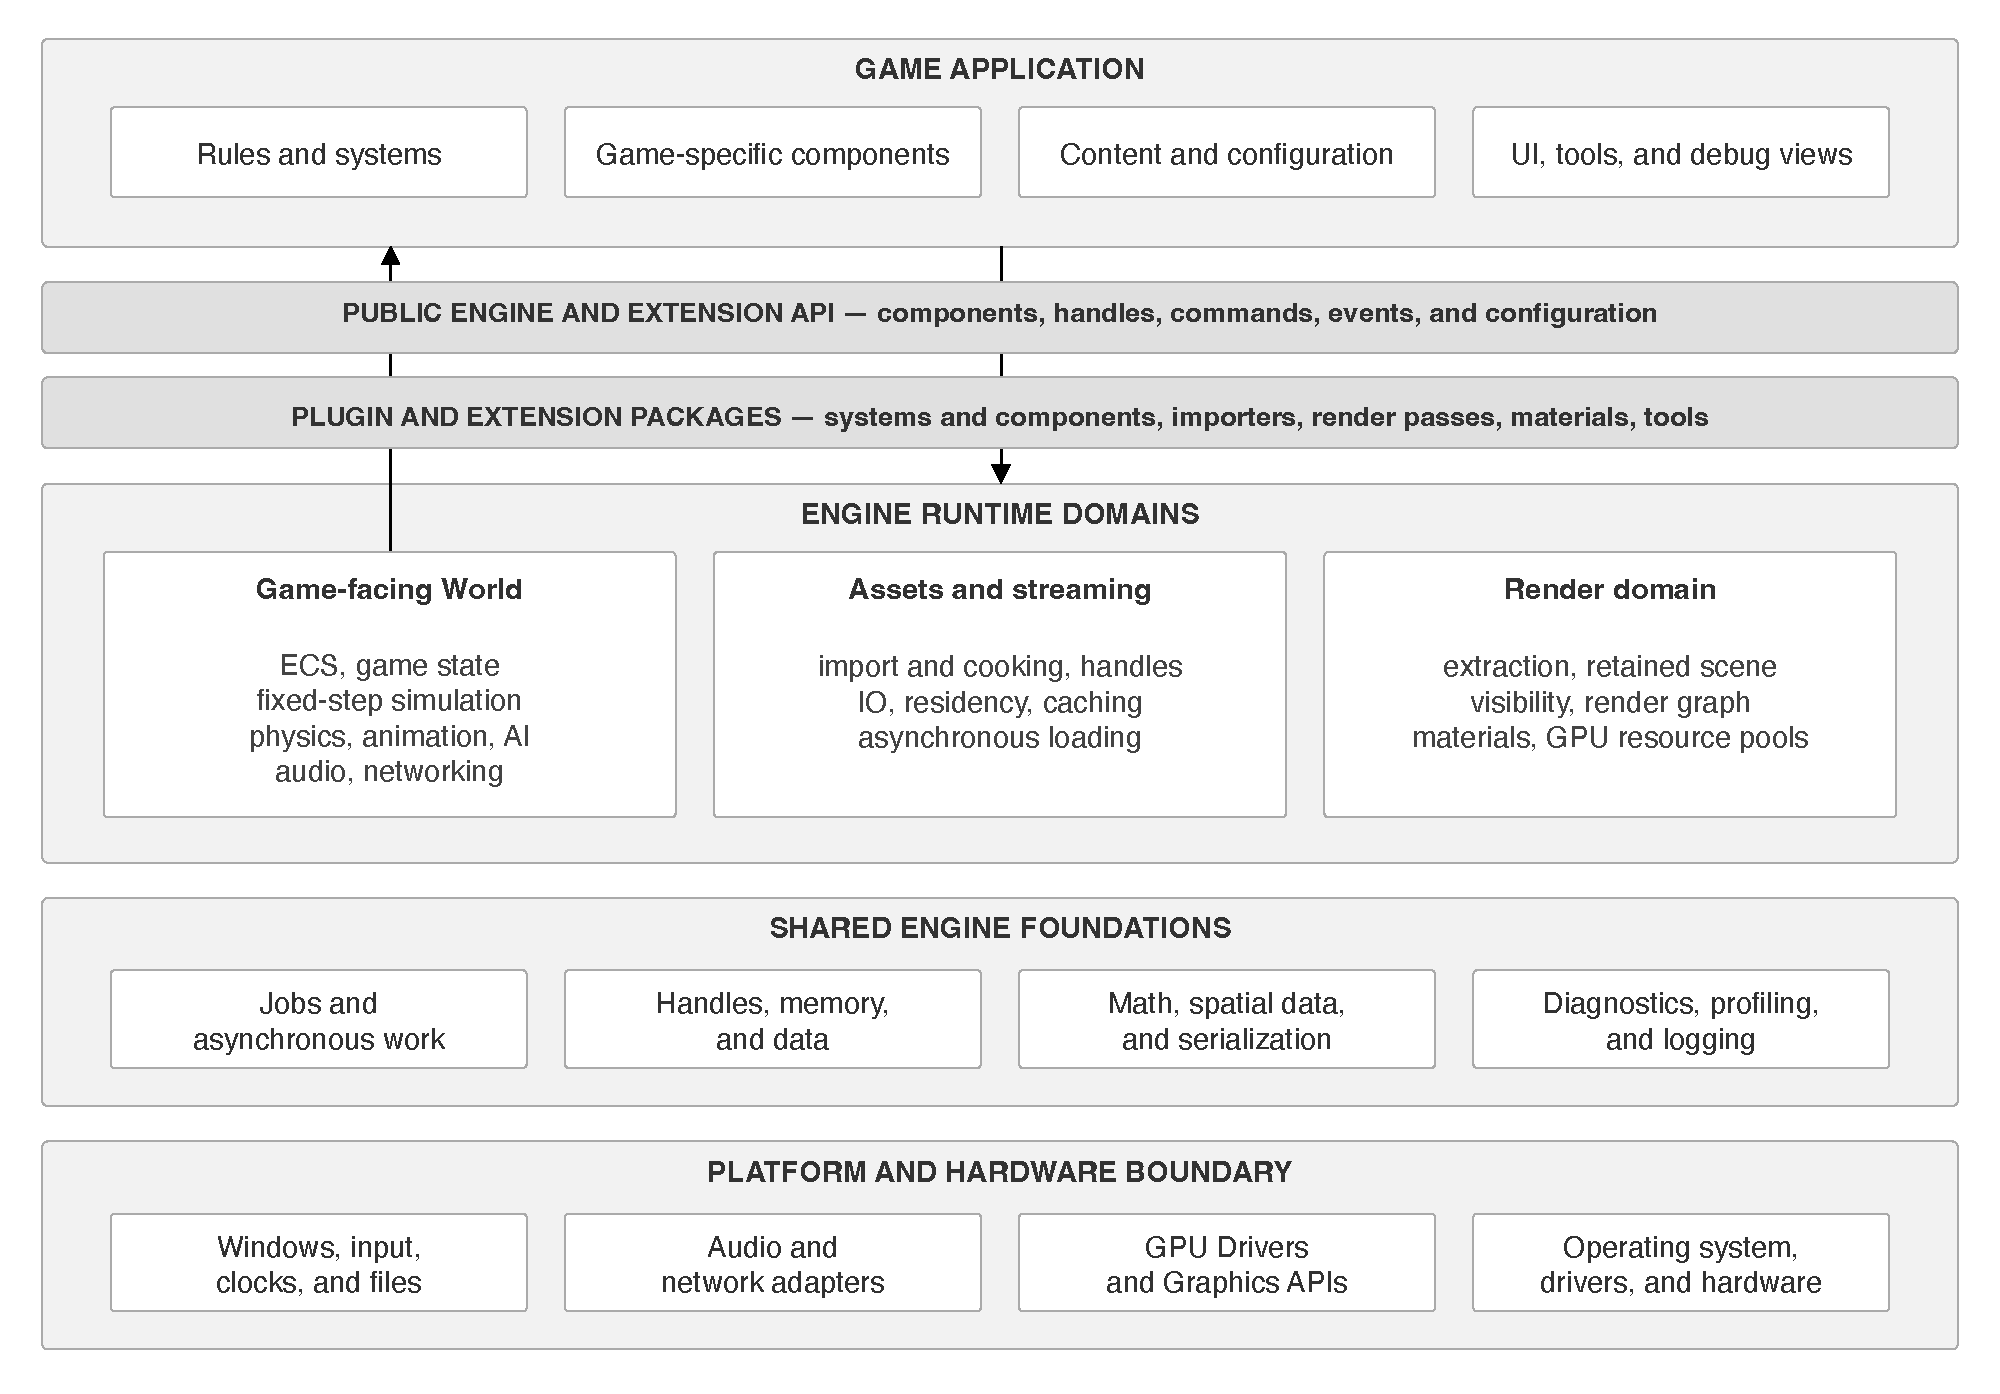
\includegraphics[width=\textwidth]{figures/engine-package-map.pdf}\par}
\caption{A conceptual package map for a modern game engine. Public and extension APIs give games controlled ways to add capabilities; runtime domains cooperate through explicit data, ownership, and scheduling contracts.}
\label{fig:engine-package-map}
\end{figure}

The three runtime domains have deliberately different jobs: The
\textbf{game-facing World} represents mutable game state and simulation;
\textbf{assets and streaming} decide how named content is found, loaded,
and kept resident; and the \textbf{render domain} turns extracted
descriptions into GPU work. They use the shared layer for mechanisms
such as jobs, handles, data structures, and diagnostics, but retain
ownership of their own state. Platform code stops at the bottom band,
where \texttt{wgpu} contains the graphics backends alongside the window,
audio, file, and network adapters.

The plugin band identifies the controlled ways a game can expand the
engine. A plugin may register component types and systems, an asset
importer or processor, a render pass or material implementation, or a
tool panel. Each extension receives the narrow contract appropriate to
its role; it does not receive arbitrary access to private renderer
state, platform handles, or another domain's mutable data. This makes
customization a first-class design feature without dissolving the
boundaries the map establishes.

The shared foundation layer at the bottom of the runtime band deserves a
note. Types such as math primitives, generational handles, a job
scheduler, logging, and profiling instrumentation are used by multiple
domains but do not carry game state or rendering state. They belong to
no single domain; they belong to all of them. Placing them in a shared
crate (or set of crates) prevents circular dependencies: the World crate
and the Render crate can both depend on the Foundation crate without
depending on each other. This is a common pattern across engines. Unreal
Engine's \texttt{Core} module provides similar shared infrastructure
(containers, math, delegates, logging) that every other module depends
on without introducing horizontal coupling between unrelated systems.

The map is deliberately a map of \emph{responsibilities}, not a call
graph. It says which concerns belong together and where a dependency may
terminate; it does not imply unrestricted access between components. The
next three subsections examine the most important divisions in that map:
the game-facing World, the engine services around it, and the
enforcement of the layers themselves.

\subsection{The Game-Facing World}\label{the-game-facing-world}

The \textbf{World} is the engine's model of the running game. It holds
entities, components, system state, and the data that game rules are
allowed to inspect and change. A common modern realization is an
entity-component-system (ECS) model: entities are stable IDs, components
are plain data, and systems operate over queries. This choice keeps
composition and bulk processing explicit. Chapter 3 establishes the
general data and ownership contracts; Chapter 8 examines ECS and the
game-facing World in depth.

The World is not the entire engine, and one of the most common
architectural mistakes in engine design is treating it as though it
were. The temptation is real: the World already has an entity system, a
query mechanism, and a way to attach data to identities. Why not put the
GPU device handle in a ``singleton component''? Why not store decoded
texture caches as a resource in the World? Why not let the streaming
system track its residency state as components on the entities it
manages?

The answer is that each of these decisions turns the World into a God
Object. When GPU handles live in the World, every subsystem that queries
the World can accidentally depend on the renderer's internal
representation. When texture caches live in the World, changing the
caching strategy requires updating every query that touches cached data.
When streaming state lives in the World, the streaming system's internal
decisions (which chunks to evict, which LOD to request) become visible
to gameplay code that has no business knowing about them. The World
becomes the place where all subsystems meet, and changing any subsystem
means changing the World's layout, which means auditing every other
subsystem that queries it.

The correct boundary is clear: the World should represent game state and
provide the stable, game-facing API through which gameplay changes that
state. GPU handles, render caches, staging pools, and streaming queues
belong in engine-side structures that the game never sees. The renderer
can then change its hardware strategy without rewriting game rules, and
the streaming system can evolve its eviction policy without touching
gameplay queries. Gregory discusses this separation extensively in the
context of keeping game-object models focused on gameplay composition
rather than engine plumbing {[}3{]}.

\subsection{Engine Services}\label{engine-services}

The services surrounding the World solve problems that are real but not
game-specific:

\begin{itemize}
\tightlist
\item
  \textbf{Asset and streaming services} turn source files into versioned
  assets, resolve handles, manage residency, and move data through IO,
  CPU memory, staging memory, and GPU memory.
\item
  \textbf{The render domain} maintains render-side state, determines
  visibility, builds draw work, records commands, and presents an image.
\item
  \textbf{Physics, audio, networking, and persistence} have their own
  update rates and external contracts. They exchange compact data with
  the World rather than borrowing arbitrary pieces of it indefinitely.
\item
  \textbf{Tools and diagnostics} observe, inspect, profile, and author
  the engine. They are a production subsystem, not an afterthought.
\end{itemize}

These services do not all need the same internal representation. A
game-facing World benefits from data structures that make gameplay
composition and queries clear; a renderer, cache, or streaming queue may
instead benefit from dense purpose-built storage. The render domain, for
example, maintains its own retained scene graph organized for spatial
traversal and draw-call batching. The asset system maintains its own
registry of loaded resources indexed by handle. The streaming
coordinator maintains its own priority queues ordered by distance and
importance. None of these structures need to be ECS archetypes, and
forcing them into the World's component model would obscure their access
patterns and reduce their performance.

This is the central distinction: organize game data around gameplay
composition; organize engine internals around their actual access
patterns. Confusing the two is a common and costly mistake. When an
engine tries to use the same ECS representation for both gameplay and
rendering, it either compromises gameplay composition (by adding
renderer-specific fields to gameplay components, polluting the game's
data model) or compromises rendering performance (by scattering
GPU-relevant data across archetype tables designed for gameplay
queries). The correct approach is to let each domain choose the
representation that serves its workload and define explicit translation
points between them. Chapters 3 and 8 return to that distinction, first
as a contract and then as a concrete game-object model.

\subsection{Layers Become Enforceable
Boundaries}\label{layers-become-enforceable-boundaries}

The diagram becomes architecture only when package structure makes it
enforceable. A healthy dependency direction flows from game-facing
concepts toward engine implementation and then toward platform adapters,
not back upward.

The omitted connections in Figure \ref{fig:engine-package-map} are as
important as its visible bands: neither the game nor the World imports a
graphics API or the private render implementation. When game code can
import renderer internals, a convenient one-off feature often becomes a
permanent coupling. A programmer adds a quick call to the renderer's
frustum-culling function to decide whether a sound effect should play.
The call works, and because it works, it stays. Six months later, the
team wants to restructure the culling system, but removing that function
signature would break gameplay code. Convenience became a dependency,
and the dependency became a constraint on future evolution.

When the World can allocate GPU resources, every future renderer change
must preserve gameplay's access to those resources. When platform types
leak upward through the layers, a windowing-library upgrade requires
touching gameplay code. Unreal Engine prevents this through its module
dependency system: game modules declare their dependencies explicitly,
and the build system rejects cycles. Godot prevents it through server
encapsulation: the \texttt{RenderingServer} owns its internal state and
exposes only opaque resource IDs (RIDs) to the scene tree. The mechanism
differs, but the principle is the same.

Smallworld realizes this rule with a public game-facing API, opaque
handles, and a render domain that owns the graphics interface. In Rust,
this enforcement is structural: the game crate depends on the public API
crate, which re-exports only the types the game may use. The render
crate is a sibling, not a dependency of the game crate. Attempting to
import a render-internal type from game code produces a compile error,
not a code-review comment. Later chapters will introduce the specific
\texttt{wgpu} types that make this boundary concrete. The durable rule
is language-independent: platform details should terminate at a narrow
adapter layer rather than leak through the game model.

The cost of maintaining these boundaries is not zero. When a game
programmer wants a quick visual effect, the fastest path is often to
call the renderer directly. When a tool needs to display a debug
overlay, the fastest path is to grab the GPU device and issue draw
calls. Each shortcut is small and individually harmless. Collectively,
they erode the boundary until it no longer provides its guarantees. An
architecture that makes the shortcuts physically impossible (through
module visibility, crate boundaries, or build-system enforcement) is
more durable than one that relies on discipline alone. This is why the
omitted connections in the package map are design decisions, not
oversights.

\section{An Engine in Time: Boot and the Main
Loop}\label{an-engine-in-time-boot-and-the-main-loop}

The package map answers what the engine contains and which dependencies
it permits. It does not yet answer when those domains come into
existence or how they make progress. That is the second architectural
question: the engine lifecycle gives it a temporal shape as illustrated
in Figure \ref{fig:engine-lifecycle}. First the engine establishes the
environment in which the game can run; then it repeats a coordinated
cycle of simulation, presentation, and service work until the
application closes. The exact order and number of threads differ among
engines, but the responsibilities are remarkably consistent.

\begin{figure}[!tb]
{\centering
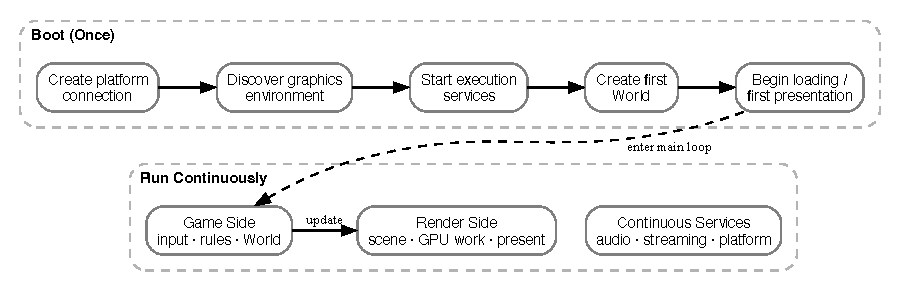
\includegraphics[width=\textwidth]{figures/engine-lifecycle.pdf}\par}
\caption{Engine lifecycle: a linear boot sequence establishes the runtime, then the main loop cycles three concurrent workstreams until shutdown.}
\label{fig:engine-lifecycle}
\end{figure}

\subsection{Boot Once: Establish the
Runtime}\label{boot-once-establish-the-runtime}

When a game starts, it hands the engine a configuration struct
(specifying window mode, rendering policy, initial content, and
performance budgets) and an application object containing the game's
specific behavior. The engine then establishes its runtime in a
dependency-aware order:

\begin{enumerate}
\def\labelenumi{\arabic{enumi}.}
\tightlist
\item
  \textbf{Create the platform connection.} The engine obtains a native
  window or display surface, starts receiving operating-system events,
  and establishes clocks and file access.
\item
  \textbf{Discover the graphics environment.} It asks the available
  graphics adapters what they support: formats, memory limits,
  presentation modes, and optional features. The engine selects a
  suitable device and configures rendering paths that fit those
  capabilities. This is why a modern renderer is not simply a fixed list
  of effects: it adapts its implementation to the machine it is running
  on.
\item
  \textbf{Start execution services.} The engine prepares its job
  workers, message queues, diagnostics, and any dedicated execution
  contexts used for rendering, audio, or asynchronous IO. Input is
  collected into an engine-owned buffer; audio and rendering services
  receive the command paths through which the game will later request
  work.
\item
  \textbf{Create the first World.} The engine invokes the game's
  initialization code and constructs an initial world from a description
  such as a menu scene, a level, or a loading screen. That description
  identifies entities and assets, rather than requiring every texture,
  mesh, sound, and world cell to be resident immediately.
\item
  \textbf{Begin loading and prepare the first presentation.} Asset work
  proceeds from storage into CPU memory, through decoding and
  processing, and (where required) into graphics memory. The engine can
  show a loading screen, menu, or placeholder scene while this work
  continues. The important point is that the first World can already be
  alive and responsive while its content becomes available.
\end{enumerate}

This ordering is not arbitrary. It is dependency-aware: each step relies
only on resources established by earlier steps. Get the ordering wrong
and circular dependencies appear. A common example: the renderer needs
the asset system to load compiled shaders, but the asset system needs
the renderer's staging pool to upload texture data into GPU memory. If
both try to initialize simultaneously, each blocks waiting for the
other. The solution is to recognize the asymmetry: the renderer can be
initialized with a minimal set of built-in shaders (compiled into the
binary or loaded from a known path) before the asset system comes
online. The asset system can then register the staging pool as an upload
target after the renderer has created it. Dependency-ordered
initialization makes this sequencing explicit, while ad-hoc ``lazy
init'' patterns hide the ordering behind opaque first-use checks that
can silently break when a new subsystem changes the order of first
access.

\floattop

\begin{codelisting}

\caption{\label{lst-engine-config}EngineConfig: the game's declaration
of engine preferences}

\centering{

\begin{Shaded}
\begin{Highlighting}[]
\KeywordTok{struct}\NormalTok{ EngineConfig }\OperatorTok{\{}
\NormalTok{    title}\OperatorTok{:}           \DataTypeTok{String}\OperatorTok{,}
\NormalTok{    window\_mode}\OperatorTok{:}\NormalTok{     WindowMode}\OperatorTok{,}
\NormalTok{    fixed\_timestep}\OperatorTok{:}  \DataTypeTok{f32}\OperatorTok{,}
\NormalTok{    pipeline\_mode}\OperatorTok{:}\NormalTok{   PipelineMode}\OperatorTok{,}
\NormalTok{    pacing}\OperatorTok{:}\NormalTok{          PacingConfig}\OperatorTok{,}
\NormalTok{    render\_budget}\OperatorTok{:}\NormalTok{   RenderBudget}\OperatorTok{,}
\NormalTok{    log\_level}\OperatorTok{:}\NormalTok{       LogLevel}\OperatorTok{,}
\OperatorTok{\}}
\end{Highlighting}
\end{Shaded}

}

\end{codelisting}%

The same principle applies at a smaller scale within each step. When the
engine creates the graphics device, it must request the features and
limits that later subsystems will need. If the renderer requests
compute-shader support but the asset system also needs compute shaders
for GPU-accelerated texture compression, the feature request must
account for both consumers. A dependency-ordered boot makes these
requirements visible: each subsystem declares what it needs, and the
boot sequence aggregates those declarations before creating the device.
The alternative, where subsystems discover missing features at first use
and crash or silently degrade, produces bugs that depend on the order in
which the player happens to trigger features.

The historical parallel is instructive. Early engines often initialized
subsystems in whatever order the main function listed them, relying on
the programmer to remember the correct sequence. Adding a new subsystem
meant finding the right insertion point by trial and error. Unreal
Engine's module system improved on this with explicit module
dependencies and a topological initialization order. Godot's server
architecture improved on it differently: each server initializes
independently because it owns its state and communicates through
messages rather than shared initialization-time references. Smallworld
follows the explicit-dependency approach, where the boot sequence is a
known, tested, linear order that can be debugged by reading a single
function.

Listing~\ref{lst-engine-config} shows the configuration struct that the
game passes to the engine at the entry point, declaring its preferences
for window mode, simulation rate, rendering policy, and performance
budgets.

By the end of boot, the engine owns the runtime infrastructure and the
World. The game has not surrendered authorship of its rules; rather,
control has inverted. The engine now calls game code at defined
lifecycle points and gives it the narrow game-facing context needed at
each point. This inversion of control is central to the engine's
architecture and deserves careful examination, which we provide in the
contracts section below. Chapter 3 explains the ownership boundaries
that make this inversion safe.

\subsection{Run Continuously: Advance, Present, and
Respond}\label{run-continuously-advance-present-and-respond}

Once boot is complete, the engine enters its main loop. A useful
high-level reading is that three kinds of work proceed together:

\begin{itemize}
\tightlist
\item
  \textbf{The game side} receives buffered input, advances time, runs
  game rules and simulation, updates the World, and issues requests such
  as ``play this sound'' or ``load this asset.'' Fixed-rate simulation
  work and frame-rate update work may occur at different cadences; the
  next chapter explains why.
\item
  \textbf{The render side} receives a description of the current scene,
  prepares the resources needed to draw it, records graphics work, and
  presents an image in the window. It may be rendering a slightly
  earlier game state while the game side is already preparing the next
  one.
\item
  \textbf{Continuous services} keep working alongside both: audio mixes
  small blocks of sound samples, streaming reads and prepares content,
  jobs finish in the background, and the platform delivers resize,
  focus, and shutdown events. UI belongs to this loop as well: it
  consumes input, changes game-visible state, and is composed into the
  presented image.
\end{itemize}

This cycle is not merely ``update, then draw.'' It is a coordination
problem across work with different rates, different latency
requirements, and different owners. Simulation may advance at a stable
60 Hz; frames arrive when the display and graphics work allow; audio
must produce samples continuously at 48 kHz regardless of frame rate;
streaming must respect memory and bandwidth budgets while the player
moves. A resize must be handled even when simulation is paused; audio
must continue producing samples even when no frame is presented;
streaming must proceed even when the renderer is stalled on a GPU fence.

The solution, adopted in some form by every modern engine, is a fixed
phase structure: a defined sequence of named phases that repeat each
tick, where each phase has a known owner, a known set of inputs, and a
known set of outputs. Figure \ref{fig:main-loop-phases} shows the two
phase sequences that form Smallworld's main loop.

\begin{figure}[!tb]
\centering
\begin{tikzpicture}[>=Latex, x=1cm, y=1cm]
  % Game tick label
  \node[font=\sffamily\bfseries\scriptsize, anchor=east] at (0.4,1.4) {Game tick};

  % Game tick phases
  \node[engine-package, text width=1.15cm, minimum height=0.7cm] (gi) at (1.2,1.1) {\textbf{Input}\\\tiny drain events};
  \node[engine-package, text width=1.15cm, minimum height=0.7cm] (gf) at (2.9,1.1) {\textbf{Fixed}\\\tiny physics, sim};
  \node[engine-package, text width=1.15cm, minimum height=0.7cm] (gu) at (4.6,1.1) {\textbf{Update}\\\tiny game logic};
  \node[engine-package, text width=1.15cm, minimum height=0.7cm] (gl) at (6.3,1.1) {\textbf{Late}\\\tiny propagate};
  \node[engine-package, text width=1.15cm, minimum height=0.7cm] (ge) at (8.0,1.1) {\textbf{Extract}\\\tiny build packet};
  \node[engine-package, text width=1.15cm, minimum height=0.7cm] (gc) at (9.7,1.1) {\textbf{Clear}\\\tiny reset tracker};
  \draw[-Latex, line width=0.4pt] (gi.east) -- (gf.west);
  \draw[-Latex, line width=0.4pt] (gf.east) -- (gu.west);
  \draw[-Latex, line width=0.4pt] (gu.east) -- (gl.west);
  \draw[-Latex, line width=0.4pt] (gl.east) -- (ge.west);
  \draw[-Latex, line width=0.4pt] (ge.east) -- (gc.west);

  % Render tick label
  \node[font=\sffamily\bfseries\scriptsize, anchor=east] at (0.4,-0.8) {Render tick};

  % Render tick phases
  \node[engine-package, text width=1.15cm, minimum height=0.7cm] (rr) at (1.2,-1.1) {\textbf{Receive}\\\tiny wait packet};
  \node[engine-package, text width=1.15cm, minimum height=0.7cm] (rp) at (2.9,-1.1) {\textbf{Prepare}\\\tiny upload, delta};
  \node[engine-package, text width=1.15cm, minimum height=0.7cm] (rc) at (4.6,-1.1) {\textbf{Cull}\\\tiny visibility};
  \node[engine-package, text width=1.15cm, minimum height=0.7cm] (rd) at (6.3,-1.1) {\textbf{Record}\\\tiny GPU cmds};
  \node[engine-package, text width=1.15cm, minimum height=0.7cm] (rs) at (8.0,-1.1) {\textbf{Submit}\\\tiny queue};
  \node[engine-package, text width=1.15cm, minimum height=0.7cm] (rp2) at (9.7,-1.1) {\textbf{Present}\\\tiny swapchain};
  \draw[-Latex, line width=0.4pt] (rr.east) -- (rp.west);
  \draw[-Latex, line width=0.4pt] (rp.east) -- (rc.west);
  \draw[-Latex, line width=0.4pt] (rc.east) -- (rd.west);
  \draw[-Latex, line width=0.4pt] (rd.east) -- (rs.west);
  \draw[-Latex, line width=0.4pt] (rs.east) -- (rp2.west);

  % Channel transfer
  \draw[-Latex, line width=0.55pt] (ge.south) -- node[right, font=\sffamily\tiny, align=left] {owned\\packet} (rr.north);

  % Feedback
  \draw[-Latex, line width=0.4pt, dashed] (rp2.north west) to[bend left=14] node[above, font=\sffamily\tiny] {feedback} (gi.south);
\end{tikzpicture}
\caption{The game tick and render tick as fixed phase sequences. Each phase has a known owner and a known set of inputs and outputs. The two ticks run on separate threads, synchronized only by the owned packet transfer at the Extract/Receive boundary. Chapter~4 defines the exact timing, pacing, and lifecycle rules.}
\label{fig:main-loop-phases}
\end{figure}
\FloatBarrier


The \textbf{game tick} runs on the Game Thread. It drains platform
events into a polled snapshot (Input), advances deterministic simulation
at a fixed rate (Fixed), runs frame-rate-dependent game logic (Update),
propagates derived state such as hierarchies and bounds (Late), builds
an owned render-facing description of the current frame (Extract), and
resets change tracking for the next tick (Clear). The \textbf{render
tick} runs on a dedicated Render Thread. It waits for the game tick's
packet (Receive), applies deltas to its private retained scene
(Prepare), determines what each camera can see (Cull), records GPU
commands through the render graph (Record), submits them (Submit), and
presents the image to the display (Present). The two ticks overlap: the
Game Thread prepares frame N+1 while the Render Thread draws frame N.
They synchronize only at the Extract/Receive boundary, where an owned
value transfers through a bounded channel.

Each phase reads only what the previous phase produced. No phase reaches
back into a previous phase's private state. The ordering is an
invariant, not a suggestion: if Extract ran before Late, the packet
would contain stale hierarchy data; if Update ran before Fixed, game
logic would see last tick's physics state. Chapter 4 defines the exact
timing rules, pacing policy, and lifecycle event handling in detail. For
now, the important architectural observation is that the main loop's
coordination role is what motivates the contracts between domains.
Without explicit contracts, the scheduler cannot reason about what each
domain needs, what it produces, and when it is safe to hand control to
the next consumer.

\section{Contracts Between Domains}\label{contracts-between-domains}

The package map names the engine's domains; the lifecycle diagram shows
them becoming active. Contracts govern the traffic between them. Without
explicit contracts, a useful package layout quickly degenerates into
every subsystem reaching into every other subsystem's state, reproducing
exactly the entangled dependency graph that the layered architecture was
supposed to prevent.

At this level, three contracts matter more than the exact queue, data
structure, or thread count:

\begin{enumerate}
\def\labelenumi{\arabic{enumi}.}
\tightlist
\item
  \textbf{Data crosses a boundary in a representation chosen for its
  consumer.}
\item
  \textbf{The engine owns runtime control and calls game code at defined
  phases.}
\item
  \textbf{Ownership, feedback, and exceptional events remain explicit.}
\end{enumerate}

The following sections explain the reasoning behind those contracts and
trace them through concrete examples. Later chapters turn each into
concrete Rust types, queues, phases, and performance budgets.

\subsection{Data Contracts: Translate Intent, Do Not Share
Internals}\label{data-contracts-translate-intent-do-not-share-internals}

The same logical thing takes different forms as it moves through an
engine. Consider the journey of a mesh from creation to screen. An
artist authors a tree model in a 3D modeling tool and exports it as a
source file (FBX, glTF, or a proprietary format). The engine's asset
pipeline imports that source data, processes it (optimizing the vertex
layout, generating LOD levels, compressing textures, building a bounding
volume), and produces a cooked asset stored in the engine's content
directory. When a game system spawns an entity with a
\texttt{MeshRenderer} component, it provides an
\texttt{AssetHandle\textless{}Mesh\textgreater{}} that names the cooked
asset. The asset system resolves that handle: if the asset is not yet
resident, it schedules a load; if it is resident, it returns a reference
to the CPU-side mesh data. During the extract phase, the engine reads
the entity's transform and mesh handle and writes them into a
\texttt{FramePacket} entry that the render domain will consume. The
render domain receives this entry and translates it into its own
retained representation: a draw command referencing a GPU vertex buffer,
an index buffer, a material pipeline, and a set of bind groups. Finally,
the command encoder records the draw call, and the GPU executes it.

Each of these transformations crosses a boundary and changes
representation. The source file becomes a cooked asset (crossing the
authoring-to-runtime boundary). The cooked asset becomes a handle in the
World (crossing the asset-to-gameplay boundary). The handle and
transform become a FramePacket entry (crossing the game-to-render
boundary, which Chapter 3 will call the Game-Render Firewall). The
FramePacket entry becomes a GPU draw command (crossing the
render-domain-to-hardware boundary). At no point does a downstream
consumer see the upstream representation directly. The game never
handles raw vertex data. The renderer never reads the live World. The
GPU never references the asset system's internal registry.

Notice what each boundary buys. Because the game holds only a handle,
the asset system is free to evict the mesh from CPU memory after
uploading it to the GPU, or to replace it with a lower-LOD version,
without the game's knowledge. Because the renderer receives an extracted
description rather than a live World reference, it can reorder, batch,
or cull draw commands without concern for simulation side effects.
Because the GPU receives recorded commands rather than pointers into the
renderer's data structures, the renderer can double-buffer its state or
reorganize its memory pools between frames. Each boundary is a point of
freedom: the implementation on either side can change independently, so
long as the representation at the boundary remains stable.

This translation is valuable for two reasons. First, game code can
express \emph{what it wants} (a mesh, material, sound, light, or
streaming request) without knowing where its bytes live or which
hardware feature will realize it. Second, the receiving subsystem can
organize the data around its own access pattern: sequential rendering
work, background IO, real-time audio mixing, or spatial queries. The
result is less coupling and fewer accidental promises about memory
layout, timing, or platform capabilities.

The boundary between simulation and rendering is the clearest example.
The game side supplies an owned description of the scene it wants
presented; the render side converts that description into graphics work
without reading or mutating the live World. Smallworld calls its version
of this handoff a \texttt{FramePacket}, but the durable lesson is
independent of that name: cross a domain boundary with a deliberate,
self-contained representation. Unreal Engine's \texttt{FSceneProxy}
mechanism, which copies game-thread data into renderer-owned proxies,
follows the same principle {[}8{]}. Godot's \texttt{RenderingServer}
accepts resource IDs and drawing commands through a message-like
interface, keeping its internal scene representation private {[}12{]}.
Chapter 3 establishes why this game-render firewall is necessary; the
rendering chapters later develop its packet and render-scene
implementation.

\subsection{Control Contracts: The Engine Drives the
Game}\label{control-contracts-the-engine-drives-the-game}

Data flows downward through increasingly specialized representations.
\textbf{Control flows differently.} The platform starts the engine; the
engine owns the main loop; and the engine calls game code at defined
lifecycle points. This inversion of control lets the runtime coordinate
input, simulation, rendering, audio, streaming, UI, and shutdown without
letting any individual game feature take over the process.

To understand why inversion of control matters, consider the
alternative. In a \textbf{library model}, the game owns the main loop
and calls engine services as needed:

\begin{verbatim}
// Library model: game owns the loop
loop {
    let input = input_lib::poll();
    game.update(input);
    let scene = game.build_scene();
    renderer::draw(scene);      // blocks until GPU finishes
    audio::mix();               // missed if draw was slow
    streaming::tick();           // starved if mix ran long
}
\end{verbatim}

This works for simple cases, but it breaks down as complexity grows. Who
decides when to poll input relative to simulation? Who ensures that
audio gets its samples on time even when a frame is slow? Who handles a
window resize that arrives between \texttt{update} and \texttt{draw}?
Who coordinates shutdown so that saves flush before the IO system is
torn down? In the library model, the game programmer must solve all of
these coordination problems manually, and each new subsystem adds a new
interaction to manage. The library model also prevents the engine from
overlapping work across frames. Because the game owns the call sequence,
it cannot allow the renderer to work on frame N while simulation
prepares frame N+1; that would require the engine to schedule both
activities, which the library model does not permit.

The pattern is familiar from other domains. A web framework like Rails
or Django does not let the application own the HTTP request loop; the
framework receives the request and calls the application's handler at a
defined point. A GUI toolkit does not let the application own the event
loop; the toolkit dispatches events and calls the application's
callbacks. The reason is the same in all cases: when the runtime must
coordinate multiple concurrent concerns (HTTP pipelining, event
delivery, UI repainting), centralized control over the loop is the only
tractable design. Game engines discovered this independently, but the
underlying principle is identical.

In the \textbf{engine model}, the engine owns the loop and calls game
code at defined phases. Listing~\ref{lst-app-trait} shows the trait that
a game implements to participate in the engine's lifecycle, along with
the engine's entry point that takes ownership of the loop.

\begin{codelisting}

\caption{\label{lst-app-trait}The App trait: the engine calls game code,
not the other way around}

\centering{

\begin{Shaded}
\begin{Highlighting}[]
\KeywordTok{trait}\NormalTok{ App }\OperatorTok{\{}
    \KeywordTok{fn}\NormalTok{ init(}\OperatorTok{\&}\KeywordTok{mut} \KeywordTok{self}\OperatorTok{,}\NormalTok{ ctx}\OperatorTok{:} \OperatorTok{\&}\KeywordTok{mut}\NormalTok{ GameContext)}\OperatorTok{;}
    \KeywordTok{fn}\NormalTok{ update(}\OperatorTok{\&}\KeywordTok{mut} \KeywordTok{self}\OperatorTok{,}\NormalTok{ ctx}\OperatorTok{:} \OperatorTok{\&}\KeywordTok{mut}\NormalTok{ GameContext}\OperatorTok{,}\NormalTok{ dt}\OperatorTok{:} \DataTypeTok{f32}\NormalTok{)}\OperatorTok{;}
    \KeywordTok{fn}\NormalTok{ fixed\_update(}\OperatorTok{\&}\KeywordTok{mut} \KeywordTok{self}\OperatorTok{,}\NormalTok{ ctx}\OperatorTok{:} \OperatorTok{\&}\KeywordTok{mut}\NormalTok{ GameContext}\OperatorTok{,}\NormalTok{ fixed\_dt}\OperatorTok{:} \DataTypeTok{f32}\NormalTok{)}\OperatorTok{;}
    \KeywordTok{fn}\NormalTok{ shutdown(}\OperatorTok{\&}\KeywordTok{mut} \KeywordTok{self}\NormalTok{)}\OperatorTok{;}
\OperatorTok{\}}

\KeywordTok{impl}\NormalTok{ Engine }\OperatorTok{\{}
    \KeywordTok{fn}\NormalTok{ run(config}\OperatorTok{:}\NormalTok{ EngineConfig}\OperatorTok{,}\NormalTok{ app}\OperatorTok{:} \KeywordTok{impl}\NormalTok{ App }\OperatorTok{+} \OtherTok{\textquotesingle{}static}\NormalTok{) }\OperatorTok{{-}\textgreater{}} \OperatorTok{!;}
\OperatorTok{\}}
\end{Highlighting}
\end{Shaded}

}

\end{codelisting}%

The \texttt{run} function's return type, \texttt{-\textgreater{}\ !}
(Rust's ``never'' type), signals that the engine takes permanent
ownership of the process. The game does not get control back after
calling \texttt{run}. This is the structural expression of inversion of
control: the game provides its behavior through the \texttt{App} trait,
and the engine decides when to invoke each method.

The game therefore provides rules, content, configuration, and
extensions. The engine decides when to poll input, when simulation may
advance, when to invoke gameplay systems, when to ask for a scene
description, and when to present an image. A game can customize the
engine through the registered extension seams in
Figure\textasciitilde{}\ref{fig:engine-package-map}, but those
extensions participate in the engine's schedule rather than creating
private loops or bypassing ownership boundaries.

Listing~\ref{lst-game-context-ch2} shows the context struct that the
engine passes to the game at each lifecycle callback. The game receives
mutable access to the World and to command-issuing services (assets,
audio, events) but only immutable access to platform state (input, time,
window). This asymmetry is deliberate: the game observes the external
environment but does not control it.

\begin{codelisting}

\caption{\label{lst-game-context-ch2}GameContext: what the game receives
at each phase}

\centering{

\begin{Shaded}
\begin{Highlighting}[]
\KeywordTok{struct}\NormalTok{ GameContext}\OperatorTok{\textless{}}\OtherTok{\textquotesingle{}a}\OperatorTok{\textgreater{}} \OperatorTok{\{}
\NormalTok{    world}\OperatorTok{:}  \OperatorTok{\&}\OtherTok{\textquotesingle{}a} \KeywordTok{mut}\NormalTok{ World}\OperatorTok{,}
\NormalTok{    input}\OperatorTok{:}  \OperatorTok{\&}\OtherTok{\textquotesingle{}a}\NormalTok{ Input}\OperatorTok{,}
\NormalTok{    time}\OperatorTok{:}   \OperatorTok{\&}\OtherTok{\textquotesingle{}a}\NormalTok{ Time}\OperatorTok{,}
\NormalTok{    assets}\OperatorTok{:} \OperatorTok{\&}\OtherTok{\textquotesingle{}a} \KeywordTok{mut}\NormalTok{ AssetServer}\OperatorTok{,}
\NormalTok{    audio}\OperatorTok{:}  \OperatorTok{\&}\OtherTok{\textquotesingle{}a} \KeywordTok{mut}\NormalTok{ AudioCommands}\OperatorTok{,}
\NormalTok{    events}\OperatorTok{:} \OperatorTok{\&}\OtherTok{\textquotesingle{}a} \KeywordTok{mut}\NormalTok{ EventBus}\OperatorTok{,}
\NormalTok{    window}\OperatorTok{:} \OperatorTok{\&}\OtherTok{\textquotesingle{}a}\NormalTok{ WindowState}\OperatorTok{,}
\OperatorTok{\}}
\end{Highlighting}
\end{Shaded}

}

\end{codelisting}%

This distinction matters because the engine must reconcile incompatible
cadences. Simulation may advance at a stable rate; frames arrive when
the display and graphics work allow; audio must produce samples
continuously; streaming and asset processing may take much longer than
one frame. Without centralized control, each subsystem would need to
negotiate its own scheduling with every other subsystem, and the result
would be the same tangled dependency graph that the layered architecture
was designed to prevent. Chapter 4 defines those schedules and the
associated pacing policy. Chapter 5 examines the input phase in detail,
showing how platform events are quarantined into a polled snapshot that
the engine provides to game code as the immutable \texttt{input} borrow
in \texttt{GameContext}.

\subsection{Feedback and Lifecycle Contracts: Make the Reverse Path
Deliberate}\label{feedback-and-lifecycle-contracts-make-the-reverse-path-deliberate}

Most useful work moves from game intent toward platform effects: World
changes become a presented image, an audio request becomes sound, and a
streaming request becomes resident content. Some information must travel
back, but it should return as \textbf{feedback}, not as a hidden
backdoor into another domain's state.

Consider what happens without explicit feedback. The game spawns an
entity and requests a mesh load. The asset system begins loading the
mesh from disk. How does the game know when the mesh is ready? In a
naive design, the game polls the asset system every frame: ``is my mesh
loaded yet?'' This works, but it means the game must track every pending
request and retry every frame. Worse, if the load fails (corrupted file,
missing dependency, exceeded memory budget), the game discovers the
failure only when it polls, and the error information is limited to
``not loaded.'' An explicit feedback contract inverts this: the asset
system sends a completion event (or a failure event with diagnostic
information) through a defined channel, and the game processes it during
a known phase. The game does not need to poll; it receives notification.
The error is rich: ``asset \texttt{tree\_oak\_01} failed to load because
texture \texttt{bark\_diffuse} exceeded the streaming budget by 4 MB.''

The same principle applies to rendering feedback. The renderer can
report GPU frame timing, memory pressure, occlusion query results, and
dynamic-resolution decisions. This information travels back to the game
side through a dedicated feedback channel, not through shared mutable
state. The game can use it to adjust quality settings, spawn fewer
particles, or warn the player that performance is degraded. The renderer
does not need to know what the game does with the information; the game
does not need to know how the renderer measured it. The feedback
contract defines the vocabulary and the delivery mechanism; each domain
retains its internal freedom.

Exceptional events follow similarly explicit paths. Resize, focus
changes, device loss, shutdown, asset failure, and budget pressure are
not ordinary gameplay data, and they cannot wait behind a stalled frame.
A window resize, for example, invalidates the GPU's swap chain and
requires the renderer to reconfigure its surface. If this event is
queued behind ordinary gameplay data and the gameplay tick is slow, the
user sees a stretched or corrupted image for several frames. Treating
resize as a first-class lifecycle event with its own delivery channel
keeps the engine responsive when normal work is paused, backpressured,
or recovering. Chapter 4 returns to these cases with a detailed
lifecycle event protocol; streaming, rendering, audio, and tooling
chapters explain their domain-specific consequences.

\subsection{Ownership: The Contract Beneath the
Others}\label{ownership-the-contract-beneath-the-others}

The data, control, and feedback contracts are all expressions of a
deeper rule: ownership. At first glance, a package diagram and a
lifecycle diagram appear to describe different things. They are both
statements about who may create, mutate, and retire state.

\begin{itemize}
\tightlist
\item
  The \textbf{World} owns mutable game state.
\item
  The \textbf{asset system} owns residency and loading policy.
\item
  The \textbf{render domain} owns device-local GPU resources and command
  submission.
\item
  The \textbf{audio domain} owns its mixer and real-time callback state.
\item
  The \textbf{platform layer} owns native windows, event pumps, and
  device integration.
\end{itemize}

When one domain needs something another owns, it receives a handle, an
immutable view, or an owned message, never an unrestricted mutable
reference. This rule sounds simple, but decades of C++ engine
development demonstrate how easily it is violated. In a traditional C++
engine, a mesh loaded by the asset system might be wrapped in a
\texttt{std::shared\_ptr\textless{}Mesh\textgreater{}} and held by three
different owners: the asset cache (so the mesh can be reused), the World
(so the entity can reference it), and the GPU resource pool (so the
renderer can draw it). Each owner believes it has a legitimate claim to
the mesh's lifetime. The result is unpredictable destruction timing.
When the entity is removed from the World, its \texttt{shared\_ptr}
drops, but the mesh persists because the asset cache and GPU pool still
hold references. When the asset cache is flushed, the mesh persists
because the GPU pool still holds a reference. The mesh is logically
freed but never reclaimed. Worse, if the GPU pool is destroyed before
the asset cache (a destruction-order bug that is easy to introduce
during refactoring), the mesh's destructor may attempt to release a GPU
buffer through a device that no longer exists, producing a crash that
only appears during shutdown.

Rust's ownership model makes this class of bug unrepresentable {[}6{]}.
A value has one owner. References are either shared and immutable or
exclusive and mutable, never both at once. Transferring ownership is
explicit (a \texttt{move}). When a domain sends data across a boundary,
the type system ensures that the sender can no longer access it. The
engine does not need conventions, code review, or runtime checks to
enforce ownership discipline; the compiler rejects violations before the
program runs. This does not mean that Rust eliminates all
resource-management complexity (GPU resources still need explicit
lifetime management through handles and arenas), but it does mean that
the most common ownership violations in C++ engines are compile-time
errors in Rust.

The handle-based alternative avoids the \texttt{shared\_ptr} problem
entirely. Instead of sharing a \texttt{Mesh} object among three owners,
the asset system owns the mesh and issues an opaque
\texttt{AssetHandle\textless{}Mesh\textgreater{}}. The World stores the
handle (a lightweight generational index, typically 8 bytes). The render
domain receives the handle as part of the extracted scene description.
When the render domain needs the mesh's GPU data, it looks up the handle
in its own resource pool, where it has already uploaded the vertex and
index buffers. No domain shares a pointer to the mesh object. No domain
can extend the mesh's lifetime by forgetting to release a reference. If
the asset system decides to evict the mesh, it invalidates the handle;
the next lookup returns a ``not resident'' result, and the game or
renderer can respond with a fallback. Destruction timing is
deterministic because there is exactly one owner.

This pattern is not unique to Rust or to Smallworld. Unreal Engine's RHI
layer uses resource handles internally for GPU objects. Godot's servers
use RID (Resource ID) integers as the only externally visible reference
to internal resources. The handle pattern has been the standard in
high-performance systems (database connection pools, file descriptor
tables, GPU resource managers) for decades. What Rust adds is
compile-time enforcement: attempting to share a mutable reference where
a handle was expected is a type error, not a code-review finding.

\subsection{Smallworld's Guiding
Principles}\label{smallworlds-guiding-principles}

Smallworld records the architectural commitments introduced in this
chapter as five guiding principles. They are not a substitute for the
domain contracts above; they are a compact way to carry those contracts
into later design decisions:

\begin{enumerate}
\def\labelenumi{\arabic{enumi}.}
\tightlist
\item
  \textbf{Data-driven game state.} The game-facing World uses entities,
  plain-data components, and systems over queries rather than a primary
  inheritance hierarchy.
\item
  \textbf{Thread ownership.} Each execution context owns its mutable
  state; work crosses the major boundaries through explicit messages and
  narrowly defined sharing rules.
\item
  \textbf{Game-render firewall.} The renderer owns device-local
  resources and command submission; the World supplies an extracted,
  render-relevant description rather than live mutable game state.
\item
  \textbf{Handle-based resources.} Games hold stable, opaque references
  while the engine owns loading, residency, caching, and GPU
  representation.
\item
  \textbf{Named budgets.} Frame time, memory, upload bandwidth, and
  streaming range are explicit, observable limits with a defined policy
  when the limit is reached.
\end{enumerate}

These five principles recur throughout the book. Each later chapter will
show how its domain realizes or depends on one or more of these
commitments, what failure modes the commitment prevents, and how the
implementation makes the commitment concrete.

The fifth principle, named budgets, deserves particular emphasis because
it is the one most often left implicit in engine design. Every engine
has budgets, whether or not it acknowledges them. GPU memory is finite.
Upload bandwidth per frame is finite. The number of draw calls the GPU
can execute within a 16.67 ms frame is finite. When these limits are
implicit, the engine runs normally during development and fails
unpredictably in production: a level with one too many unique textures
triggers an out-of-memory crash; a streaming system that was fast enough
during testing saturates the upload queue when the player moves quickly
through a dense area. Making budgets explicit (a \texttt{RenderBudget}
with a stated triangle count, a \texttt{StreamingBudget} with a stated
bytes-per-frame limit, a \texttt{MemoryBudget} with a stated pool size)
transforms these silent failures into observable, debuggable events. The
engine can report ``streaming budget exceeded by 12 MB'' rather than
crashing with ``out of memory'' in an allocation whose call stack is
three subsystems removed from the cause.

\section*{Chapter Summary}\label{chapter-summary-1}
\addcontentsline{toc}{section}{Chapter Summary}

\markright{Chapter Summary}

A modern engine is best understood as a group of cooperating ownership
domains rather than a feature checklist. This chapter established the
architectural map that the rest of the book will zoom into:

\begin{enumerate}
\def\labelenumi{\arabic{enumi}.}
\item
  \textbf{Organization.} The engine is divided into a game-facing World,
  a set of engine services (rendering, assets, streaming, physics,
  audio, tools), a shared foundation layer, and a platform adapter band.
  Dependencies flow downward; the omitted upward connections are as
  architecturally significant as the ones drawn. The layered pattern
  emerged historically because engines that allowed unrestricted
  cross-layer access could not be ported, maintained, or extended.
\item
  \textbf{Lifecycle.} The engine boots in a dependency-aware order
  (platform, graphics discovery, execution services, World creation,
  initial loading) and then enters a main loop where game-side
  simulation, render-side presentation, and continuous services (audio,
  streaming, IO) proceed concurrently. The main loop is a coordination
  problem, not a sequential pipeline.
\item
  \textbf{Contracts.} Three contracts govern inter-domain traffic. The
  data contract requires that information crossing a boundary adopt a
  representation chosen for its consumer, not a shared internal format.
  The control contract inverts the traditional library relationship: the
  engine owns the loop and calls game code at defined phases, rather
  than the game calling engine services directly. The ownership contract
  ensures that domains communicate through handles, immutable views, or
  owned messages, never shared mutable references. Rust's type system
  makes ownership violations compile-time errors rather than runtime
  bugs.
\item
  \textbf{Guiding principles.} Smallworld carries these contracts as
  five named commitments: data-driven game state, thread ownership, the
  game-render firewall, handle-based resources, and named budgets.
\end{enumerate}

The following chapters are guided zooms into this map.

\textbf{Engine Runtime Contracts} (Chapter 3) defines the World-render
firewall, the hybrid data model, and thread ownership contracts.

\textbf{Core Loop and Frame Lifecycle} (Chapter 4) defines how the
domains advance in time, pace frames, and respond to lifecycle events.

\textbf{Input and Platform Interaction} (Chapter 5) traces the path from
raw platform signals to game-facing intent. Subsequent chapters on
resources, streaming, rendering, physics, animation, audio, networking,
and tools each examine a specific domain and its contracts with the rest
of the engine. Readers should return to this chapter's map whenever a
later subsystem introduces a new handle, thread, queue, or package.

The design question is always the same: which domain owns this state,
and what is the smallest explicit contract through which another domain
may use it?

\section*{Review Questions}\label{review-questions-1}
\addcontentsline{toc}{section}{Review Questions}

\markright{Review Questions}

\begin{enumerate}
\def\labelenumi{\arabic{enumi}.}
\item
  Why does an engine architecture need explicit contracts between
  domains, rather than letting each subsystem access whatever data it
  needs? Describe a concrete failure that results from the absence of
  such contracts.
\item
  Trace the path of a mesh from authored source data to a visible pixel.
  Name each domain boundary the data crosses and how its representation
  changes at each boundary.
\item
  The chapter describes inversion of control: the engine calls game
  code, not the other way around. What would break if the game owned the
  main loop and called engine services as a library? Give at least two
  coordination problems that the library model cannot solve cleanly.
\item
  Why should the game-facing World not contain GPU handles, render
  caches, or streaming state? What antipattern results if it does, and
  how does it affect the engine's ability to evolve its renderer
  independently of gameplay?
\item
  The five guiding principles include ``named budgets.'' Give an example
  of a budget that, if left implicit, could cause a failure that is
  difficult to diagnose. Explain how making that budget explicit changes
  the failure from a crash into a debuggable event.
\item
  Boot order is dependency-aware. Describe a circular dependency that
  could arise between the renderer and the asset system, and explain how
  the engine resolves it without resorting to lazy initialization.
\item
  The ownership contract states that domains communicate through
  handles, immutable views, or owned messages rather than shared mutable
  references. How does Rust's type system make this contract enforceable
  at compile time? Contrast this with how a C++ engine would enforce the
  same contract.
\item
  The chapter's package map (Figure \ref{fig:engine-package-map}) omits
  certain connections deliberately. Pick one omitted connection (for
  example, game code importing renderer internals) and explain what
  architectural damage would result if it were allowed.
\end{enumerate}

\chapter{Runtime Contracts}\label{runtime-contracts}

Chapter 2 established three architectural questions: how the engine is
organized into domains, how those domains come alive at boot and in the
main loop, and which contracts let them cooperate without sharing their
internals. This chapter is the first guided zoom into those contracts.
It concentrates on the two with the greatest structural consequences:
the \textbf{data contract}, which defines the representations that may
cross a domain boundary, and the \textbf{ownership contract}, which
defines who may mutate state on either side.

Those contracts become three closely connected questions:

\begin{enumerate}
\def\labelenumi{\arabic{enumi}.}
\tightlist
\item
  How does the game-facing World describe rendering intent without
  exposing renderer internals?
\item
  How is game state represented and composed so gameplay can evolve
  without making the whole engine share one object model?
\item
  Which execution context owns mutable state, and how do domains
  communicate when work must cross that ownership boundary?
\end{enumerate}

Get any of these wrong and the consequences compound: tangled coupling,
synchronization hazards, cache-hostile memory layouts, and an
ever-growing surface of subtle bugs that ship to players. These are not
theoretical risks. The history of game engine development is, in large
part, a history of discovering these failure modes one shipped title at
a time and building architectural defenses against them.

We begin with the \textbf{Game-Render Firewall}, the data boundary that
decouples simulation logic from GPU presentation. We then examine
\textbf{Data-Oriented Composition}: why ECS is the modern representation
for the game-facing World, rather than a traditional object-oriented
hierarchy. Finally, we explore \textbf{Thread Ownership}, the principle
that each execution context exclusively owns its mutable data and
communicates through explicit messages. Together, the firewall,
data-driven composition, and thread ownership make Chapter 2's data and
ownership contracts concrete. The next chapter turns to the remaining
control and lifecycle contract: when each domain advances, how frames
are paced, and how resize, device loss, and shutdown remain responsive.

\section*{What You Will Learn in This
Chapter}\label{what-you-will-learn-in-this-chapter-2}
\addcontentsline{toc}{section}{What You Will Learn in This Chapter}

\markright{What You Will Learn in This Chapter}

\begin{itemize}
\tightlist
\item
  \textbf{The Game-Render Firewall:} Why game code should not see GPU
  resources, what an explicit extraction contract protects, and why
  renderer-owned state is essential to safe overlap.
\item
  \textbf{Data-Oriented Composition:} Why ECS is the modern answer to
  representing game objects: entities as identities, components as data,
  and systems as operations over that data.
\item
  \textbf{Thread Ownership and CSP Messaging:} How Rust's ownership
  system makes shared mutability explicit and bounded, and why the
  engine uses Communicating Sequential Processes (CSP) channels for its
  main cross-thread boundaries.
\item
  \textbf{Work-Stealing Pools:} Why the engine splits its worker pools
  into game and render tiers, how this prevents priority inversion, and
  why a unified task-graph scheduler is the planned evolution rather
  than the starting architecture.
\item
  \textbf{Handle-Based Resource Management:} The role of generational
  indices, \texttt{SlotMap} arenas, and opaque handles in providing
  safe, cache-friendly resource access without garbage collection or
  reference counting on hot paths.
\end{itemize}

\section{The Game-Render Firewall}\label{the-game-render-firewall}

One of the most consequential architectural decisions in a
multi-threaded game engine is the boundary between simulation and
presentation. This boundary did not appear in engine designs all at
once; it was discovered through accumulated pain. Early engines ran
everything on a single thread in a single loop, and the renderer simply
read whatever state it needed from the live world. That worked until
hardware changed the economics.

The transition began in the late 1990s and early 2000s, as GPUs became
powerful enough to justify dedicating a thread to feeding them. id
Software's engine lineage illustrates the trajectory: Doom's renderer
was tightly coupled to its BSP traversal and column-drawing code, making
it impossible to change the rendering strategy without rewriting
gameplay-adjacent systems. By the time id Tech 4 shipped with \emph{DOOM
3} (2004), the engine had introduced a distinct front-end/back-end split
in the renderer, separating the scene description from the low-level
draw-call submission. When Unreal Engine 3 introduced a dedicated Render
Thread for \emph{Gears of War} (2006), the separation became a
first-class architectural contract: the Game Thread produced scene data,
the Render Thread consumed it, and neither was permitted to touch the
other's private state. That contract has survived every subsequent
Unreal generation since then because it solves a problem that does not
go away with faster hardware - it actually gets worse.

\subsection{The Problem: Coupling Limits
Concurrency}\label{the-problem-coupling-limits-concurrency}

In a naive single-threaded engine, the game loop is a monolithic
sequence: read input, update the world, build draw calls, submit to the
GPU, present. Every subsystem has implicit access to everything else.
The renderer reads entity transforms directly from the world. The world
queries GPU readback buffers for occlusion data. Materials are modified
in the same function that evaluates AI behavior.

Consider what happens when a team tries to parallelize this engine
without first establishing a boundary. A gameplay programmer stores a
raw GPU buffer pointer inside a component so that a particle system can
write directly to device memory. The optimization works: particles
update faster because they skip the staging copy. Six months later, the
team decides to overlap simulation and rendering across frames. Now the
particle system's GPU write races with the renderer's command recording
on a different thread. The team adds a mutex. The mutex serializes the
particle update and the renderer, erasing most of the overlap benefit.
Worse, when the team later ports to a platform with a different graphics
API, every component that stored a GPU handle must be rewritten, because
the handle type has changed. A single shortcut, storing a GPU buffer
pointer in a gameplay component, has created coupling that limits
concurrency, complicates profiling, and increases the cost of every
future platform change.

Figure \ref{fig:single-thread-coupling} illustrates why this becomes a
structural problem: the same live state serves both the world update and
renderer, so neither can progress independently without synchronization.

\begin{figure}[!tb]
\centering
\begin{tikzpicture}[>=Latex, node distance=0.55cm]
  \node[engine-layer, minimum width=14.5cm, minimum height=3.9cm] (box) {};
  \node[font=\sffamily\bfseries\scriptsize, anchor=north] at (box.north) [yshift=-0.28cm] {SINGLE-THREADED, SHARED-STATE LOOP};
  \node[engine-package, minimum width=1.9cm, minimum height=0.65cm] (input) at (-5.2,0.60) {Input};
  \node[engine-package, minimum width=2.2cm, minimum height=0.65cm, right=of input] (world) {World update};
  \node[engine-package, minimum width=2.2cm, minimum height=0.65cm, right=of world] (draws) {Build draws};
  \node[engine-package, minimum width=1.4cm, minimum height=0.65cm, right=of draws] (gpu) {GPU};
  \draw[-Latex, line width=0.5pt] (input) -- (world);
  \draw[-Latex, line width=0.5pt] (world) -- (draws);
  \draw[-Latex, line width=0.5pt] (draws) -- (gpu);
  \node[engine-package, text width=3.4cm, minimum height=1.05cm, align=left] (state) at (-1.0,-0.95) {\textbf{Shared live state}\\Entity transforms\\GPU buffers\\Material state};
  \draw[-Latex, dashed, line width=0.5pt] (world.south) -- (state.north west);
  \draw[-Latex, dashed, line width=0.5pt] (draws.south) -- (state.north east);
\end{tikzpicture}
\caption{A naive shared-state loop. When world update and draw preparation both access live state, concurrent progress requires synchronization.}
\label{fig:single-thread-coupling}
\end{figure}
\FloatBarrier


\subsection{The Extraction Contract}\label{the-extraction-contract}

Every major engine that ships overlapped simulation and rendering has
converged on the same structural answer: give each side its own mutable
state, and connect them with a deliberate extraction step.

Unreal Engine 5 realizes this with a hard split: the \textbf{Game
Thread} owns the world, and the \textbf{Render Thread} owns the GPU.
Between them sits \texttt{FSceneProxy}, a mechanism that copies the data
the renderer needs into renderer-owned proxies. The two threads then
operate independently, overlapped by one frame {[}8{]}. Godot takes a
different but convergent approach: the \texttt{RenderingServer} owns all
rendering state behind a message-like API, and the scene tree
communicates with it through opaque resource IDs (RIDs) rather than
direct object references {[}12{]}. Despite their different languages and
architectures, both engines arrived at the same structural conclusion:
\textbf{the renderer must own its state, and the game must not alias
it}.

This is the \textbf{Game-Render Firewall}: extract a render-relevant
view from the live world, transfer it across a narrow boundary, and let
the render domain own the resulting state. The extract step is the
boundary. Everything above it speaks in transforms, materials, and
handles; everything below it speaks in draw commands and GPU resources.
Game code describes intent and the renderer translates that intent into
hardware work.

The firewall's narrow invariant is precise: the Render Thread
exclusively owns device-local resources and command submission. Nothing
outside the render domain should allocate a device-local buffer, write
to a render target, or submit GPU commands. In Smallworld, Rust's type
system enforces this structurally: game code never sees a
\texttt{wgpu::Device}, a bind group, or a GPU buffer. The Game Thread
sends owned messages through a bounded channel; the Render Thread
receives them into a retained scene it alone may mutate.

The firewall constrains \emph{game code}, not engine internals. Engine
subsystems, including the asset pipeline, the staging pool, and the
streaming coordinator, may create and populate CPU-visible staging
resources from any thread. What they may not do is touch device-local
memory or record render commands.

This distinction matters: asset loading and streaming can proceed
concurrently without violating the thread-safety contract, because they
operate only on staging memory that the render domain later consumes. In
Smallworld, \texttt{wgpu}'s internally-synchronized \texttt{Device} and
\texttt{Queue} handles make this safe by design; in Unreal, staging
uploads similarly run on any thread while only the Render Thread records
final GPU commands. Figure \ref{fig:game-render-firewall} makes the
resulting ownership and transfer rule explicit.

\begin{figure}[!tb]
\centering
\begin{tikzpicture}[>=Latex]
  \node[engine-layer, minimum width=14.5cm, minimum height=2.15cm] (game) at (0,2.25) {};
  \node[font=\sffamily\bfseries\scriptsize, anchor=north] at (game.north) [yshift=-0.27cm] {GAME DOMAIN};
  \node[engine-package, text width=12.6cm, minimum height=1.0cm] at (0,1.92) {\textbf{Owns:} World state, game logic, entity hierarchies\\\textbf{Speaks in:} transforms, materials, handles, events, and commands\\\textbf{Never touches:} GPU devices, bind groups, render targets, or command encoders};
  \node[engine-boundary, text width=7.1cm, minimum height=0.62cm] (extract) at (0,0.72) {EXTRACT --- owned render description};
  \draw[-Latex, line width=0.6pt] (game.south) -- (extract.north);
  \node[font=\sffamily\scriptsize, align=left, anchor=west] at (3.95,0.72) {views, lights, geometry and material intent,\\resource requests, extension descriptions};
  \node[engine-layer, minimum width=14.5cm, minimum height=2.15cm] (render) at (0,-1.25) {};
  \node[font=\sffamily\bfseries\scriptsize, anchor=north] at (render.north) [yshift=-0.27cm] {RENDER DOMAIN};
  \node[engine-package, text width=12.6cm, minimum height=1.0cm] at (0,-1.58) {\textbf{Owns:} render-side scene, GPU pools, render targets, command submission\\\textbf{Speaks in:} draw commands, GPU resources, shader bindings\\\textbf{Never touches:} World, components, or live game state};
  \draw[-Latex, line width=0.6pt] (extract.south) -- (render.north);
\end{tikzpicture}
\caption{The Game--Render Firewall. An owned, render-relevant description crosses from the mutable game World to the renderer; private mutable state does not.}
\label{fig:game-render-firewall}
\end{figure}
\FloatBarrier


A reasonable engineer might ask: why not use read-write locks or atomics
to share state between threads instead of copying data? Modern
concurrency tools make shared access safe; why add the overhead of owned
messages? The answer is that shared mutable state defeats three
properties that a clean boundary provides:

\begin{enumerate}
\def\labelenumi{\arabic{enumi}.}
\item
  \textbf{Coherent render view.} When the Game Thread transfers an owned
  render description, the Render Thread processes a frozen view of the
  world at a known point in time. There are no races over
  partially-updated state. The renderer never sees a half-applied
  physics step or a transform that was modified after the camera was
  positioned. This does not, by itself, make simulation deterministic;
  but it makes the simulation-to-render handoff coherent and repeatable.
\item
  \textbf{Profiling and isolation.} Each thread's work can be traced,
  timed, and optimized in complete isolation. A game-thread stall does
  not pollute render-thread timings. A GPU bottleneck is visible in
  render-thread metrics without any game-thread interference. When the
  two domains share mutable state, profiling becomes archaeology: you
  reconstruct causality from interleaved lock acquisitions, and the
  performance team loses hours isolating which thread caused a spike.
\item
  \textbf{Evolutionary safety.} When the renderer needs a new piece of
  data, say a per-entity wind reactivity scalar, the change is surgical:
  add it to the published description and teach the renderer how to
  consume it. The game side and render side never see each other's
  private changes. When data is shared through a thread-safe reference
  count or a lock-protected struct, adding a field requires auditing
  every reader and writer across every thread simultaneously. The blast
  radius of a change is the entire codebase.
\end{enumerate}

The pattern has a useful analogy outside game engines. In database
architecture, a common strategy for scaling read-heavy workloads is to
replicate the primary database to read replicas. Writes go to the
primary; reads go to a replica that holds a consistent, slightly-behind
snapshot. The replica never writes back to the primary's tables, and the
primary never reads the replica's query cache. The separation imposes
replication cost but buys independence: the primary can compact,
re-index, or migrate without touching the read path, and the read
replicas can be scaled, cached, or replaced without affecting writes.
The game-render firewall serves the same structural purpose: the World
is the primary (writes), the render scene is the replica (reads), and
the extraction step is the replication channel.

Unreal Engine enforces this boundary through convention, documentation,
and code review. A determined (or careless) programmer can reach across
it, and the resulting bug may not manifest until a specific timing
coincidence on a specific hardware configuration. In Rust, an owned
description can be made \texttt{Send} while containing no references
into the World. Once sent, the Game Thread cannot read it. Once
received, the Render Thread cannot reach back. Here the type system is
the enforcement mechanism, not human discipline.

\subsection{General Properties and
Cost}\label{general-properties-and-cost}

The extraction contract can be realized by many different mechanisms: a
renderer may receive a complete snapshot, only changes since the
previous handoff, or a mixture of both. It may use a message queue, a
double buffer, or another bounded transfer owned by the engine.
Regardless of mechanism, the contract needs four properties:

\begin{enumerate}
\def\labelenumi{\arabic{enumi}.}
\item
  The game domain publishes \textbf{an owned, render-relevant
  description}, not references into its live World.
\item
  The render domain turns that description into \textbf{state it owns}.
\item
  The handoff has a documented \textbf{capacity and latency policy}, so
  a slow renderer cannot silently create an unlimited queue of obsolete
  work.
\item
  Any information that travels back is \textbf{time-stamped advisory
  feedback}, not a synchronous dependency of the current simulation
  step.
\end{enumerate}

Each mechanism has different costs for static worlds, rapidly changing
worlds, and latency-sensitive games. The architectural invariant is
independent of that choice: no domain obtains an alias to another
domain's mutable private state. Unreal Engine's scene proxies and
Godot's \texttt{RenderingServer} both express these four properties,
though through entirely different machinery {[}8, 12{]}. Chapter 12
makes those alternatives concrete through extraction, retained
render-side state, bounded handoffs, and asynchronous feedback; it then
uses Smallworld's \texttt{FramePacket} as the Rust-specific realization
rather than treating that type as the principle itself.

\textbf{The cost of this boundary is real.} Extraction duplicates
render-relevant state across the boundary, and the one-frame pipeline
overlap adds one frame of input-to-photon latency (roughly 16 ms at 60
fps). Maintaining the extraction code is ongoing work: every new
renderable component type requires a corresponding extract path. Mature
engines mitigate the duplication cost through delta extraction rather
than full-scene copies. Unreal's \texttt{FSceneProxy} objects are
created once when an actor registers with the scene; only properties
that actually changed are pushed to the render thread via dirty-marking
(calls like \texttt{MarkRenderStateDirty} and \texttt{UpdateTransform}).
Smallworld follows the same strategy: components are dirty-tracked on
mutation, and the extract step copies only changed state (Chapter 8
examines the change-tracking mechanism in detail).

In a scene with 100,000 entities where only 2,000 moved this frame, only
those 2,000 transforms cross the boundary. The cost is proportional to
change, not to scene size. These costs are real but justified, because
the alternative, shared mutable state between simulation and rendering,
produces worse outcomes at scale: serialized threads, unpredictable
profiling, and a refactoring blast radius that grows with every new
subsystem. The boundary is an investment that pays increasing dividends
as the engine grows.

\begin{tcolorbox}[enhanced jigsaw, arc=.35mm, bottomrule=.15mm, breakable, colback=white, colframe=quarto-callout-warning-color-frame, left=2mm, leftrule=.75mm, opacityback=0, rightrule=.15mm, toprule=.15mm]
\begin{minipage}[t]{5.5mm}
\textcolor{quarto-callout-warning-color}{\faExclamationTriangle}
\end{minipage}%
\begin{minipage}[t]{\textwidth - 5.5mm}

\vspace{-3mm}\textbf{Weak Game-Render Boundaries}\vspace{3mm}

\begin{itemize}
\tightlist
\item
  GPU objects in gameplay types let game rules depend on renderer
  implementation.
\item
  A synchronous readback or lock turns a supposedly asynchronous
  boundary into a hidden stall.
\item
  An unbounded queue turns a temporary render slowdown into rising
  input-to-photon latency.
\end{itemize}

Each is best prevented by the boundary design itself, not by asking
every future caller to be careful.

\end{minipage}%
\end{tcolorbox}

\section{Data-Oriented Composition at the Game
Boundary}\label{data-oriented-composition-at-the-game-boundary}

With the thread boundary established, we turn to the second foundational
question: how should the engine represent \textbf{game state}? If you
have worked on a game of any scale, you have likely encountered this
question in its painful form: a class hierarchy that was clean at first,
then grew rigid as designers asked for objects that did not fit any
existing branch of the tree. The question is not academic. It determines
how easily a game team can add new content, how efficiently the engine
can process large worlds, and whether the extraction step from the
previous section can work at all.

This is a decision about the game-facing World: the running collection
of actors, characters, vehicles, props, lights, and other things that
gameplay must compose, query, serialize, replicate, and inspect. It is
not a claim about whether the engine's renderer, asset loader, or
platform code should be written with classes, structs, or any particular
internal pattern.

The game-object question has a long and instructive history. For two
decades, game engines used deep inheritance hierarchies to model game
entities. The typical tree looked like this: a base \texttt{GameObject}
or \texttt{Entity} class provided lifecycle methods (create, update,
destroy). Subclasses added capabilities: \texttt{Renderable} added
drawing, \texttt{Collidable} added physics, \texttt{Character} added
movement, and \texttt{PlayerCharacter} added input handling. This worked
well for games where the object taxonomy was known at design time and
changed slowly. It began to fail when games needed objects that did not
fit neatly into a single branch of the tree.

The turning point came in the early 2000s. Scott Bilas, working on
\emph{Dungeon Siege} at Gas Powered Games, presented ``A Data-Driven
Game Object System'' at GDC 2002, articulating a component-based
alternative: instead of defining what an object \emph{is} through
inheritance, define what it \emph{has} through composable data
attachments {[}13{]}. The idea was not entirely new (some form of
composition appeared in earlier engines), but Bilas's talk gave the
pattern a name, a concrete implementation, and a clear argument for why
it scaled better than inheritance. The component model spread through
the industry over the following decade. Unity adopted it as
MonoBehaviour attachments. Unreal Engine evolved its Actor-Component
model into an increasingly data-oriented design. By the time Blizzard
shipped \emph{Overwatch} (2016) on a custom ECS architecture, the
pattern had proven itself at the scale of a competitive multiplayer
title with millions of concurrent players and strict networking
requirements {[}14{]}.

The two representations under discussion are a traditional
object-oriented game-object model, in which a game's things are
primarily instances in an inheritance taxonomy, and
entity-component-system (ECS), in which entities are stable identities,
components are data, and systems operate over selected component sets.
The following comparison concerns this one decision: which model gives a
modern game-facing World the clearest support for composition, bulk
queries, serialization, and change over time?

\subsection{From Class Taxonomy to
Composition}\label{from-class-taxonomy-to-composition}

Class hierarchies and component-object models have long been useful ways
to describe game objects. Unreal's \texttt{UObject}/Actor framework, for
example, combines inheritance with attachable components, reflection,
serialization, and editor integration. The difficulty appears when a
class taxonomy becomes the primary representation for a large,
performance-sensitive game world. Figure
\ref{fig:oop-inheritance-pyramid} shows the kind of tree that
accumulates shared behavior and lifecycle obligations downward through
every descendant.

\begin{figure}[!tb]
\centering
\begin{tikzpicture}[>=Latex, level distance=0.72cm, sibling distance=3.0cm,
  every node/.style={engine-package, minimum width=2.0cm, minimum height=0.55cm}]
  \node {\texttt{UObject}}
    child {node {\texttt{AActor}}
      child {node {\texttt{APawn}}
        child {node {\texttt{ACharacter}}
          child {node {\texttt{APlayerCharacter}}}}
        child {node {\texttt{AVehicle}}}}
      child {node {\texttt{ALight}}}};
\end{tikzpicture}
\caption{An inheritance taxonomy concentrates shared behavior and lifecycle obligations in base types. It can be useful, but does not by itself organize a large game World for composable data or bulk queries.}
\label{fig:oop-inheritance-pyramid}
\end{figure}
\FloatBarrier


To see why a deep taxonomy becomes a design constraint, consider a
concrete scenario. A game has \texttt{ACharacter} (which inherits
movement and collision from \texttt{APawn}, which inherits lifecycle
from \texttt{AActor}), and separately has \texttt{AVehicle} (which
inherits physics simulation from its own branch). A designer wants a
mech suit: a vehicle the player rides, but which also has character-like
abilities such as melee attacks and inventory. In an inheritance model,
the mech must choose a branch. If it inherits from \texttt{ACharacter},
it lacks the vehicle physics. If it inherits from \texttt{AVehicle}, it
lacks the character abilities. Multiple inheritance introduces the
diamond problem and makes method resolution ambiguous. The team's
solution is typically a large ``mech'' class that duplicates behavior
from both branches, or an increasingly complex delegation pattern that
re-invents composition inside the inheritance framework. Each workaround
adds code that must be maintained whenever either base class changes.

This hierarchy encodes behavior and shared lifecycle through inherited
types. An \texttt{APlayerCharacter} inherits movement from
\texttt{ACharacter}, which inherits collision from \texttt{APawn}, which
inherits lifecycle from \texttt{AActor}, which inherits serialization
and reflection from \texttt{UObject}. Each layer adds methods, member
variables, and invariants that all descendants must respect.

For a game-facing world that must be queried in bulk, this
representation has several costs:

\begin{enumerate}
\def\labelenumi{\arabic{enumi}.}
\item
  \textbf{A taxonomy does not compose new capabilities gracefully.}
  Adding a capability such as swimming can lead to new subclasses or
  increasingly complex component conventions. Changing a base-class
  invariant can affect every descendant.
\item
  \textbf{Bulk queries need a deliberate data layout.} In many
  object-oriented implementations, objects and their relevant fields are
  spread over individual allocations. Iterating 10,000 transforms then
  becomes pointer chasing rather than a predictable linear scan.
  Inheritance does not require this layout, but it does not naturally
  encourage storage organized around the query either.
\item
  \textbf{Hot loops benefit from direct data access.} Virtual dispatch
  is a valuable tool at extension points, but it is a poor default for a
  tight transform, visibility, or physics query that needs a few fields
  from many entities.
\item
  \textbf{Reflection is powerful but carries a system-wide cost.}
  Unreal's generated metadata enables editor tooling, serialization,
  garbage collection, and Blueprint access. It also adds generated code,
  build work, and runtime machinery that a smaller engine can avoid when
  its data model is simpler.
\item
  \textbf{Shared architecture can concentrate collaboration pressure.}
  When unrelated features meet in base classes or binary authoring
  assets, merges and reviews become more difficult than they need to be.
\end{enumerate}

\subsection{The Advantages of ECS}\label{the-advantages-of-ecs}

The same design pressures that made class taxonomies unwieldy have
driven engine after engine toward composition-based models. The
convergence is striking: Unity ships its Entities package as a full ECS
implementation. Unreal Engine's Mass Entity framework represents
high-scale gameplay entities as composable, data-only fragments
processed by data-oriented systems. Blizzard built Overwatch's gameplay
layer on a custom ECS that gave the team deterministic replay, efficient
networking, and the ability to add new hero abilities without touching
base classes {[}5, 14, 15{]}. Neither engine thereby abandons every
object-oriented API; the important conclusion is narrower and more
durable. When the question is how to represent the mutable game World,
composition of data is a better foundation than a class hierarchy. This
is Smallworld's data-driven-game-state commitment.

An entity is an opaque ID, a generational index into a \texttt{SlotMap}.
It has no type, no base class, no vtable. What makes a ``player''
different from a ``tree'' is not inheritance but the set of components
attached. Listing~\ref{lst-entity-composition} contrasts a player entity
(transform, mesh, physics, audio) with a light entity (transform, light
source) to show how the same spawn-and-attach API produces fundamentally
different game objects.

\begin{codelisting}

\caption{\label{lst-entity-composition}Composing game objects from
components}

\centering{

\begin{Shaded}
\begin{Highlighting}[]
\CommentTok{// A player: transform + mesh + physics + audio + behavior}
\KeywordTok{let}\NormalTok{ player }\OperatorTok{=}\NormalTok{ world}\OperatorTok{.}\NormalTok{spawn()}\OperatorTok{;}
\NormalTok{world}\OperatorTok{.}\NormalTok{add(}
\NormalTok{    player}\OperatorTok{,}
\NormalTok{    Transform }\OperatorTok{\{}
\NormalTok{      position}\OperatorTok{:} \PreprocessorTok{Vec3::}\NormalTok{ZERO}\OperatorTok{,}
\NormalTok{      rotation}\OperatorTok{:} \PreprocessorTok{Quat::}\NormalTok{IDENTITY}\OperatorTok{,}
\NormalTok{      scale}\OperatorTok{:} \PreprocessorTok{Vec3::}\NormalTok{ONE}\OperatorTok{,}
    \OperatorTok{\},}
\NormalTok{)}\OperatorTok{;}
\NormalTok{world}\OperatorTok{.}\NormalTok{add(}
\NormalTok{    player}\OperatorTok{,}
\NormalTok{    MeshRenderer }\OperatorTok{\{}
\NormalTok{      mesh}\OperatorTok{:}\NormalTok{ player\_mesh}\OperatorTok{,}\NormalTok{ material}\OperatorTok{:}\NormalTok{ player\_mat}\OperatorTok{,}\NormalTok{ cast\_shadows}\OperatorTok{:} \ConstantTok{true}\OperatorTok{,} \OperatorTok{..}\KeywordTok{default}\NormalTok{()}
    \OperatorTok{\},}
\NormalTok{)}\OperatorTok{;}
\NormalTok{world}\OperatorTok{.}\NormalTok{add(player}\OperatorTok{,}\NormalTok{ RigidBody }\OperatorTok{\{}\NormalTok{ mass}\OperatorTok{:} \DecValTok{80.0}\OperatorTok{,}\NormalTok{ drag}\OperatorTok{:} \DecValTok{0.1}\OperatorTok{,} \OperatorTok{..}\KeywordTok{default}\NormalTok{() }\OperatorTok{\}}\NormalTok{)}\OperatorTok{;}
\NormalTok{world}\OperatorTok{.}\NormalTok{add(player}\OperatorTok{,}\NormalTok{ AudioListener)}\OperatorTok{;}

\CommentTok{// A light: transform + light source. That\textquotesingle{}s it.}
\KeywordTok{let}\NormalTok{ sun }\OperatorTok{=}\NormalTok{ world}\OperatorTok{.}\NormalTok{spawn()}\OperatorTok{;}
\NormalTok{world}\OperatorTok{.}\NormalTok{add(}
\NormalTok{    sun}\OperatorTok{,}
\NormalTok{    Transform }\OperatorTok{\{}
\NormalTok{        position}\OperatorTok{:} \PreprocessorTok{DVec3::}\NormalTok{new(}\DecValTok{0.0}\OperatorTok{,} \DecValTok{1000.0}\OperatorTok{,} \DecValTok{0.0}\NormalTok{)}\OperatorTok{,}
        \OperatorTok{..}\KeywordTok{default}\NormalTok{()}
    \OperatorTok{\},}
\NormalTok{)}\OperatorTok{;}
\NormalTok{world}\OperatorTok{.}\NormalTok{add(}
\NormalTok{    sun}\OperatorTok{,}
\NormalTok{    LightSource }\OperatorTok{\{}
\NormalTok{        kind}\OperatorTok{:} \PreprocessorTok{LightKind::}\NormalTok{Directional }\OperatorTok{\{}
\NormalTok{          direction}\OperatorTok{:} \PreprocessorTok{Vec3::}\NormalTok{NEG\_Y}\OperatorTok{,}
\NormalTok{          cascade\_count}\OperatorTok{:} \DecValTok{4}\OperatorTok{,}
        \OperatorTok{\},}
\NormalTok{        color}\OperatorTok{:} \PreprocessorTok{Vec3::}\NormalTok{ONE}\OperatorTok{,}
\NormalTok{        intensity}\OperatorTok{:} \DecValTok{10.0}\OperatorTok{,}
\NormalTok{        cast\_shadow}\OperatorTok{:} \ConstantTok{true}\OperatorTok{,}
\NormalTok{        shadow\_bias}\OperatorTok{:} \DecValTok{0.001}\OperatorTok{,}
    \OperatorTok{\},}
\NormalTok{)}\OperatorTok{;}
\end{Highlighting}
\end{Shaded}

}

\end{codelisting}%

This is the same basic insight behind UE5's component attachment and
Mass fragments: build a game object from the capabilities it has, rather
than from the nearest branch of an inheritance tree. Smallworld realizes
that idea with plain Rust data and does not require \texttt{UObject}
reflection or \texttt{UPROPERTY} metadata for its game-object model. The
type system provides safety;
\texttt{Send\ +\ Sync\ +\ \textquotesingle{}static} is the only trait
bound on components.

The analogy to database design is instructive. A traditional
object-oriented game world stores each entity as a ``row'' in a
heap-allocated object, with all of its fields (transform, mesh, physics,
health, inventory) packed together. Iterating over all transforms means
visiting every object and extracting one field from each, which scatters
reads across memory. An ECS stores components in column-oriented arrays:
all transforms in one contiguous array, all mesh renderers in another,
all rigid bodies in a third. Iterating over all transforms is a linear
scan through packed memory. This is the same insight that led the
database industry from row-oriented stores (PostgreSQL, MySQL) to
columnar stores (Apache Arrow, DuckDB, ClickHouse) for analytical
workloads: when the query touches a few columns across many rows,
column-major layout wins because the CPU prefetcher can predict the
access pattern.

\textbf{Why plain data matters.} The ``plain data'' constraint is not
merely aesthetic; it is load-bearing:

\begin{itemize}
\item
  \textbf{Dense storage.} Components of the same type are stored in
  contiguous arrays. Iterating over every \texttt{Transform} in the
  world is a linear scan through packed memory. Compare this to chasing
  pointers through an inheritance hierarchy, where each object's
  \texttt{Transform} lives at a different heap address.
\item
  \textbf{Trivial serialization.} A plain data struct with no pointers,
  no virtual methods, and no closures can be serialized mechanically. An
  entity's full state is the union of its serializable components. No
  custom \texttt{SaveGame} overrides, no ``forgot to serialize that new
  field'' bugs. In Smallworld, \texttt{serde} derive macros generate the
  serialization code at compile time.
\item
  \textbf{Safe extraction.} The extract step takes a read-only view of
  the World. Because components are data (not behaviors that might call
  back into the world), read-only access is guaranteed to be
  side-effect-free. This is what makes the firewall compositionally
  sound: extraction cannot trigger game logic. In Rust, this guarantee
  is enforced by borrowing \texttt{\&World}, an immutable reference that
  the compiler verifies at build time.
\item
  \textbf{Deterministic change tracking.} When game code requests
  mutable access to a component, the access automatically marks that
  component dirty in a change tracker. Because components are inert
  data, there is no possibility of a mutation happening through a side
  channel; every change is visible to the tracker. In Smallworld,
  \texttt{world.get\_mut::\textless{}Transform\textgreater{}(entity)}
  returns a guarded \texttt{\&mut\ Transform} that records the write.
\end{itemize}

\subsection{The Engine/Game Component
Split}\label{the-enginegame-component-split}

A useful component model draws a clean line between \textbf{engine
components} (defined and consumed by the engine) and \textbf{game
components} (defined by each game project). Engine components such as
\texttt{Transform}, \texttt{MeshRenderer}, \texttt{LightSource}, and
\texttt{RigidBody} have semantic meaning to the engine: the extract step
can convert a \texttt{MeshRenderer} into a draw command, and the physics
system can simulate a \texttt{RigidBody}. Game components remain opaque
to the engine. Listing~\ref{lst-game-components} illustrates the
distinction: \texttt{Health} and \texttt{Inventory} attach with the same
API as engine components, but no engine system iterates over them.

\begin{codelisting}

\caption{\label{lst-game-components}Game-defined components remain
opaque to the engine}

\centering{

\begin{Shaded}
\begin{Highlighting}[]
\CommentTok{// Game{-}defined components: the engine does not know about these}
\KeywordTok{struct}\NormalTok{ Health }\OperatorTok{\{}\NormalTok{ current}\OperatorTok{:} \DataTypeTok{f32}\OperatorTok{,}\NormalTok{ max}\OperatorTok{:} \DataTypeTok{f32} \OperatorTok{\}}
\KeywordTok{struct}\NormalTok{ Inventory }\OperatorTok{\{}\NormalTok{ slots}\OperatorTok{:} \DataTypeTok{Vec}\OperatorTok{\textless{}}\DataTypeTok{Option}\OperatorTok{\textless{}}\NormalTok{ItemId}\OperatorTok{\textgreater{}\textgreater{},}\NormalTok{ capacity}\OperatorTok{:} \DataTypeTok{usize} \OperatorTok{\}}

\CommentTok{// Attach them exactly like engine components}
\NormalTok{world}\OperatorTok{.}\NormalTok{add(player}\OperatorTok{,}\NormalTok{ Health }\OperatorTok{\{}\NormalTok{ current}\OperatorTok{:} \DecValTok{100.0}\OperatorTok{,}\NormalTok{ max}\OperatorTok{:} \DecValTok{100.0} \OperatorTok{\}}\NormalTok{)}\OperatorTok{;}
\NormalTok{world}\OperatorTok{.}\NormalTok{add(player}\OperatorTok{,}\NormalTok{ Inventory }\OperatorTok{\{}\NormalTok{ slots}\OperatorTok{:} \PreprocessorTok{vec!}\NormalTok{[}\ConstantTok{None}\OperatorTok{;} \DecValTok{20}\NormalTok{]}\OperatorTok{,}\NormalTok{ capacity}\OperatorTok{:} \DecValTok{20} \OperatorTok{\}}\NormalTok{)}\OperatorTok{;}
\end{Highlighting}
\end{Shaded}

}

\end{codelisting}%

The engine iterates over its known component types during the LATE phase
(hierarchy propagation, bounds recomputation, streaming demand) and the
EXTRACT phase. Game components participate only through game-registered
systems. This split is what keeps the engine's inner loops tight: the
physics system iterates over \texttt{(RigidBody,\ Collider,\ Transform)}
tuples, not over arbitrary component sets.

\subsection{Asset Descriptors: Data-Driven Entity
Archetypes}\label{asset-descriptors-data-driven-entity-archetypes}

An entity archetype should be authorable as data rather than
reconstructed in code every time a level loads. This lets designers
change the initial composition and tuning of a game object without
editing gameplay source, and it keeps asset references out of hard-coded
constructors.

\textbf{Asset descriptors} are a lightweight realization: serializable
RON, JSON, or binary files that describe an entity archetype.
Listing~\ref{lst-enemy-descriptor} defines an \texttt{EnemyDescriptor}
with asset paths for mesh, material, and loot table alongside tuning
values for health and speed.

\begin{codelisting}

\caption{\label{lst-enemy-descriptor}A serializable descriptor for an
enemy archetype}

\centering{

\begin{Shaded}
\begin{Highlighting}[]
\KeywordTok{struct}\NormalTok{ EnemyDescriptor }\OperatorTok{\{}
\NormalTok{  mesh}\OperatorTok{:}\NormalTok{       AssetPath}\OperatorTok{,}       \CommentTok{// "meshes/goblin.glb"}
\NormalTok{  material}\OperatorTok{:}\NormalTok{   AssetPath}\OperatorTok{,}       \CommentTok{// "materials/goblin.ron"}
\NormalTok{  health}\OperatorTok{:}     \DataTypeTok{f32}\OperatorTok{,}
\NormalTok{  speed}\OperatorTok{:}      \DataTypeTok{f32}\OperatorTok{,}
\NormalTok{  loot\_table}\OperatorTok{:}\NormalTok{ AssetPath}\OperatorTok{,}
\OperatorTok{\}}
\end{Highlighting}
\end{Shaded}

}

\end{codelisting}%

The engine loads these descriptors, resolves asset paths to handles, and
spawns entities with the appropriate components. Artists and designers
edit the data files; programmers define the descriptor schemas and the
systems that process them. Because the files are text-based (RON or
JSON), they diff and merge cleanly in version control. Unreal's
Data-Only Blueprints solve the same broad authoring problem within its
editor and asset system, though their binary \texttt{.uasset}
representation makes ordinary source-control diffs less direct.

This is the data-driven principle in action: the \emph{structure} of a
goblin (what components it has, what mesh it uses, how much health it
starts with) is data. The \emph{behavior} of a goblin (how it patrols,
how it attacks) is code, either a Rust \texttt{Behavior} implementation
or a Lua script. The two concerns are cleanly separated, and either can
change independently.

\subsection{Handle-Based Resources}\label{handle-based-resources}

The next commitment completes the data-driven picture:
\textbf{handle-based resources}. Games hold opaque handles. Lifetime,
caching, and GPU upload are engine-managed.
Listing~\ref{lst-resource-handles} defines both handle types:
\texttt{AssetHandle\textless{}T\textgreater{}} for immutable shared
assets and \texttt{ResourceHandle\textless{}T\textgreater{}} for mutable
resources such as materials.

\begin{codelisting}

\caption{\label{lst-resource-handles}Opaque handles separate game
references from engine-managed lifetime}

\centering{

\begin{Shaded}
\begin{Highlighting}[]
\KeywordTok{struct}\NormalTok{ AssetHandle}\OperatorTok{\textless{}}\NormalTok{T}\OperatorTok{\textgreater{}} \OperatorTok{\{}
\NormalTok{    id}\OperatorTok{:}\NormalTok{         AssetId}\OperatorTok{,}
\NormalTok{    generation}\OperatorTok{:} \DataTypeTok{u32}\OperatorTok{,}
\NormalTok{    \_marker}\OperatorTok{:}\NormalTok{    PhantomData}\OperatorTok{\textless{}}\NormalTok{T}\OperatorTok{\textgreater{},}
\OperatorTok{\}}

\KeywordTok{struct}\NormalTok{ ResourceHandle}\OperatorTok{\textless{}}\NormalTok{T}\OperatorTok{\textgreater{}} \OperatorTok{\{}
\NormalTok{    id}\OperatorTok{:}\NormalTok{         ResourceId}\OperatorTok{,}
\NormalTok{    generation}\OperatorTok{:} \DataTypeTok{u32}\OperatorTok{,}
\NormalTok{    \_marker}\OperatorTok{:}\NormalTok{    PhantomData}\OperatorTok{\textless{}}\NormalTok{T}\OperatorTok{\textgreater{},}
\OperatorTok{\}}
\end{Highlighting}
\end{Shaded}

}

\end{codelisting}%

\begin{itemize}
\item
  \textbf{\texttt{AssetHandle\textless{}T\textgreater{}}} references an
  immutable, shared asset (mesh geometry, texture pixels, audio clips).
  Many entities can hold the same handle. The asset's GPU-resident
  representation is managed by the engine's GPU pools; game code never
  knows whether the asset is in VRAM, in the staging pool, or still
  loading from disk.
\item
  \textbf{\texttt{ResourceHandle\textless{}T\textgreater{}}} references
  a mutable resource (materials). The game can modify these at runtime,
  for example animating a material's emissive intensity or swapping a
  texture, and the \texttt{ChangeTracker} records the mutation for the
  next extract.
\end{itemize}

Both use \textbf{generational indices} for use-after-free detection.
When a resource is freed, its slot's generation counter increments. Any
handle still holding the old generation will fail a generation check on
access, producing a clean miss rather than a use-after-free crash. This
provides the safety guarantees of reference counting without the runtime
cost of atomic increment/decrement on every copy.

The pattern is not unique to game engines. Operating systems manage file
descriptors the same way: a file descriptor is an integer index into a
per-process table, not a pointer to a kernel structure. Closing a file
invalidates the descriptor; reusing the slot with a new file means that
a stale descriptor does not accidentally operate on the wrong resource.
Database connection pools, Wayland's object IDs, and GPU driver handles
all follow the same principle: give the consumer an opaque token, keep
the real resource behind a lookup table, and let the owner manage
lifetime. The pattern recurs because it solves a universal problem: when
multiple consumers need to reference a resource without extending its
lifetime or aliasing its memory, an indirected handle is the simplest
correct answer.

\textbf{The costs of data-oriented composition are worth acknowledging.}
ECS introduces indirection: accessing a component requires a lookup
through the entity's archetype, which is more complex than reading a
field from a known object pointer. Relationships between entities
(parent-child hierarchies, equipment slots, group membership) must be
modeled explicitly, typically through component fields that store entity
IDs, because ECS does not provide an inherent containment model. The
programming model is less familiar to developers coming from an
object-oriented background, and debugging a system that operates on
anonymous component tuples requires tooling support that many ECS
frameworks are still developing. These costs are real, but they are
outweighed for game-world representation at scale: the composition
flexibility, cache-friendly iteration, trivial serialization, and safe
extraction that ECS provides are difficult to retrofit into a class
hierarchy.

\begin{tcolorbox}[enhanced jigsaw, arc=.35mm, bottomrule=.15mm, breakable, colback=white, colframe=quarto-callout-tip-color-frame, left=2mm, leftrule=.75mm, opacityback=0, rightrule=.15mm, toprule=.15mm]
\begin{minipage}[t]{5.5mm}
\textcolor{quarto-callout-tip-color}{\faLightbulb}
\end{minipage}%
\begin{minipage}[t]{\textwidth - 5.5mm}

\vspace{-3mm}\textbf{Data-Driven Game Objects}\vspace{3mm}

\begin{itemize}
\tightlist
\item
  \textbf{Keep components compact.} Large components, such as an
  \texttt{Inventory} containing a heap-allocated \texttt{Vec}, erode the
  cache-locality benefit of dense storage. Put variable-size data behind
  a handle or in a side table; keep the component itself a fixed-size
  index into that data.
\item
  \textbf{Separate hot from cold data.} A \texttt{MeshRenderer} combines
  hot transform-adjacent work with a mesh handle that changes rarely.
  When profiling calls for it, separate data by update and query rate
  rather than loading cold fields on every transform update.
\item
  \textbf{Use gameplay tags for cross-system communication.} When
  several systems react to the same state, use a hierarchical tag such
  as \texttt{status.debuff.burning} instead of coupling systems through
  direct calls or special-case shared components.
\end{itemize}

\end{minipage}%
\end{tcolorbox}

\section{Thread Ownership and the Work-Stealing
Pools}\label{thread-ownership-and-the-work-stealing-pools}

The firewall establishes the boundary between two threads. But a modern
game engine is not two threads; it is a constellation of execution
contexts, each with its own responsibilities, data, and timing
constraints. If you have ever profiled a frame and found two subsystems
contending on a lock that neither should need, or traced a deadlock to
an undocumented acquisition order between a render mutex and an audio
mutex, you have experienced what happens when ownership rules are
absent. The goal is not a particular number of threads, but ownership
rules that make those failure modes difficult to express in the first
place.

The industry arrived at this understanding through hardware pressure.
For most of the 1990s, game engines ran on a single CPU core, and
threading was either unnecessary or confined to a background loading
thread. The Xbox 360 (2005), with its three dual-threaded PowerPC cores,
forced engine teams to confront multi-threading as a performance
requirement rather than an optimization. Naughty Dog's journey is
particularly instructive: their PS3-era engine used a traditional
multi-threaded model with explicit job dependencies, but by the time
\emph{The Last of Us} shipped, the complexity of managing those
dependencies had become a development bottleneck. Christian Gyrling
presented the team's response at GDC 2015: a fiber-based job system that
replaced OS threads with lightweight, cooperatively-scheduled fibers,
giving the scheduler fine-grained control over work distribution without
the overhead of OS context switches {[}16{]}. Frostbite and id Tech
evolved their own task-graph schedulers for similar reasons: as the
number of interdependent subsystems grew, ad-hoc threading became
untenable, and engines converged on explicit ownership rules with
structured concurrency.

\subsection{The Ownership Principle}\label{the-ownership-principle}

The guiding principle is \textbf{thread ownership}: each execution
context owns its mutable data, and the main cross-thread boundaries
communicate through explicit messages rather than ambient shared state.

This principle has a critical refinement: sharing \emph{immutable} data
across threads is permitted. A mesh's vertex data, once loaded, can be
referenced from any thread through a shared, read-only pointer. What no
thread may do is mutate that data while another thread holds a
reference. The rule forbids shared \textbf{mutability}, not sharing.

The principle leads to a practical test: a hot path should not need a
global read-write lock around the world, a mutex around the render
scene, or an atomic compare-and-swap loop merely to establish ordinary
ownership. If the architecture is right, each domain holds its data
outright, and work crosses boundaries through owned messages. In C++
engines, this discipline is enforced by code review and thread
sanitizers. In Rust, it is enforced by the compiler; the ``How Rust
Enables This Architecture'' subsection below explains how \texttt{Send},
\texttt{Sync}, and the borrow checker make these ownership rules
structural rather than conventional. Smallworld meets the test directly:
each domain owns its state, and bounded channels transfer ownership at
the boundaries.

\subsection{The Execution Contexts}\label{the-execution-contexts}

The engine uses six execution contexts, each with clear ownership
boundaries. For each, the critical questions are: what persistent
mutable state does it own, and how does it communicate with the rest of
the engine?

\textbf{Game Thread} (dedicated, main thread). Owns the World, input
state, time, gameplay systems, and the asset server. Sends an owned
render description to the Render Thread each frame; receives
time-stamped advisory feedback in return.

\textbf{Render Thread} (dedicated). Owns the GPU context, the retained
render scene, resource pools, and the render graph. Receives render
descriptions in; sends feedback out. Nothing outside this thread submits
GPU commands.

\textbf{Game Worker Pool} (work-stealing). Owns no persistent state;
borrows work items from the Game Thread via scoped tasks
(\texttt{join()}, \texttt{parallel\_for()}). Runs physics, animation
sampling, and streaming demand computation. The parent thread guarantees
the borrowed data outlives the task.

\textbf{Render Worker Pool} (work-stealing). Owns no persistent state;
borrows work items from the Render Thread via scoped tasks. Runs frustum
culling, draw call sorting, and batch generation. Separate from the game
pool to prevent priority inversion (discussed below).

\textbf{Streaming Coordinator} (dedicated, low priority). Owns the
demand priority queue and budget arbiter. Receives demand requests from
the Game Thread; dispatches IO and decode work to the IO pool; sends
completed \texttt{UploadBatch} messages to the Render Thread.

\textbf{Audio Thread} (dedicated). Owns the mixer, active voices, and
the platform output stream. Drains \texttt{AudioCommands} issued by the
Game Thread each frame.

\textbf{IO Pool} (blocking-friendly). Owns no persistent state. Executes
blocking filesystem reads and decompression tasks dispatched by the
asset server and streaming coordinator. Runs on a separate pool so that
disk stalls cannot starve CPU-bound game or render work.

Several design choices deserve attention. The four dedicated threads
(Game, Render, Audio, Streaming) each get their own OS thread so that
latency-sensitive work cannot be preempted by lower-priority tasks. A
physics computation on a shared pool should never cause a present-miss
on the render thread. The two worker pools are stateless by design: they
borrow bounded work and return results, which keeps scoped task
lifetimes simple and verifiable. And the IO pool is deliberately
separate from both worker pools, because a single disk stall that blocks
a game or render worker would propagate latency into the frame pipeline.

\subsection{Why Two Worker Pools?}\label{why-two-worker-pools}

The split between the game worker pool and the render worker pool is a
deliberate choice to prevent \textbf{priority inversion}. Consider a
scenario where both pools are unified. A complex physics island solve
occupies all available worker threads for 8 ms. During that window, the
Render Thread dispatches frustum culling work to the same pool. The
culling tasks, which are render-critical and must complete before
command recording can begin, sit in the queue behind physics work that
has no frame deadline. The frame misses its present target, and the
player sees a hitch. The physics work was correct and well-optimized;
the failure was a scheduling accident caused by mixing work with
incompatible priorities in the same pool.

In Figure \ref{fig:worker-pool-priority}, a render-critical culling task
misses its deadline when it shares a saturated pool with simulation;
separate pools prevent that queuing relationship.

\begin{figure}[!tb]
\centering
\begin{tikzpicture}[>=Latex]
  \node[engine-layer, minimum width=14.5cm, minimum height=2.55cm] (shared) at (0,2.35) {};
  \node[font=\sffamily\bfseries\scriptsize, anchor=north] at (shared.north) [yshift=-0.27cm] {ONE SHARED WORKER POOL};
  \foreach \x in {-4.7,-1.6,1.5,4.6} {
    \node[engine-package, minimum width=2.25cm, minimum height=0.58cm] at (\x,2.15) {Physics solve (3 ms)};
  }
  \node[engine-package, text width=4.45cm, minimum height=0.72cm] at (0,1.18) {Frustum culling (render-critical)};
  \node[font=\sffamily\scriptsize, anchor=west] at (2.35,1.18) {waits behind physics $\rightarrow$ missed frame};
  \node[font=\sffamily\bfseries\scriptsize] at (0,0.30) {SPLIT POOLS};
  \node[engine-layer, minimum width=6.75cm, minimum height=2.0cm] (game) at (-3.85,-1.15) {};
  \node[font=\sffamily\bfseries\scriptsize, anchor=north] at (game.north) [yshift=-0.25cm] {GAME WORKER POOL};
  \node[engine-package, text width=5.7cm, minimum height=1.0cm] at (-3.85,-1.48) {Physics\quad Animation\quad Streaming};
  \node[engine-layer, minimum width=6.75cm, minimum height=2.0cm] (render) at (3.85,-1.15) {};
  \node[font=\sffamily\bfseries\scriptsize, anchor=north] at (render.north) [yshift=-0.25cm] {RENDER WORKER POOL};
  \node[engine-package, text width=5.7cm, minimum height=1.0cm] at (3.85,-1.48) {Frustum culling\quad Draw sorting\quad Batch merge};
\end{tikzpicture}
\caption{Priority inversion in a shared worker pool, and the separation that prevents render-critical preparation from queueing behind game work.}
\label{fig:worker-pool-priority}
\end{figure}
\FloatBarrier


The \textbf{game pool} runs physics (the provider's internal parallelism
binds here), animation sampling, and streaming demand computation. The
\textbf{render pool} runs frustum culling, draw call sorting, and batch
generation. Because the two-frame pipeline keeps both pools concurrently
busy (the game pool works on frame N+1 while the render pool works on
frame N), the split costs little utilization. And render-critical
culling work never queues behind a heavy physics island solve.

\subsection{CSP: Communicating Sequential
Processes}\label{csp-communicating-sequential-processes}

The primary inter-thread communication model is \textbf{Communicating
Sequential Processes (CSP)}, the formal model that C. A. R. Hoare
introduced in 1978 {[}17{]}. The core idea is deceptively simple:
concurrent processes do not share memory; they communicate by sending
and receiving messages on typed channels. Each process is sequential
internally, and all coordination happens at the channel boundaries. The
model has proven durable across decades and domains: Go's goroutines and
channels, Erlang's actor mailboxes, and the message-passing interfaces
in operating system microkernels (QNX, seL4) all descend from the same
insight. The reason CSP recurs is that it eliminates shared mutable
state at the communication boundary, which is precisely where the most
difficult concurrency bugs hide.

In Smallworld, each major domain boundary gets its own typed channel:
the Game Thread sends an owned render description to the Render Thread,
receives advisory feedback in return, issues audio commands that the
Audio Thread drains each frame, and posts demand requests that the
Streaming Coordinator fulfills. Each channel carries owned values. Once
a value is sent, the sender no longer has access to it. Once received,
the receiver has exclusive ownership. Figure \ref{fig:csp-message-flow}
shows the data-plane routes.

\begin{figure}[!tb]
\centering
\begin{tikzpicture}[>=Latex, node distance=2.05cm and 4.5cm]
  \node[engine-package, minimum width=2.75cm, minimum height=0.8cm] (game) {Game Thread};
  \node[engine-package, minimum width=2.75cm, minimum height=0.8cm, right=of game] (render) {Render Thread};
  \node[engine-package, minimum width=2.75cm, minimum height=0.8cm, below=of game] (audio) {Audio Thread};
  \node[engine-package, minimum width=3.35cm, minimum height=0.8cm, below=of render] (stream) {Streaming Coordinator};
  \draw[-Latex, line width=0.55pt] (game) -- node[above, font=\sffamily\scriptsize] {render description} (render);
  \draw[-Latex, line width=0.55pt] (render.south west) to[bend right=18] node[below, font=\sffamily\scriptsize] {advisory feedback} (game.south east);
  \draw[-Latex, line width=0.55pt] (game) -- node[left, font=\sffamily\scriptsize, align=right] {\texttt{AudioCommands}} (audio);
  \draw[-Latex, line width=0.55pt] (game.south east) to[bend left=8] node[above, font=\sffamily\scriptsize] {demand} (stream.north west);
  \draw[-Latex, line width=0.55pt] (stream.north) to[bend left=10] node[right, font=\sffamily\scriptsize] {\texttt{UploadBatch}} (render.south);
\end{tikzpicture}
\caption{The primary CSP data-plane messages. Each arrow transfers a deliberately typed, owned value; lifecycle control remains on an independent channel.}
\label{fig:csp-message-flow}
\end{figure}
\FloatBarrier


Lifecycle events (window resize, device loss, shutdown) ride an
\textbf{out-of-band control channel}, separate from the render-data
plane. This follows Gregory's control/data-plane separation principle:
control must be deliverable independent of normal frame traffic {[}3{]}.
A paused game that generates no render descriptions still resizes. A
stalled pipeline that cannot accept another description still shuts
down.

\textbf{Where threads meet safely.} There is one place where the strict
``no shared mutable state'' rule bends: the \textbf{staging pool}, the
region of CPU-visible GPU memory where asset decode threads deposit data
for the renderer to upload into device-local memory. Every engine that
overlaps asset loading with rendering has a mechanism like this:
Unreal's RHI layer wraps it behind \texttt{RHIStagingBuffer} and
fence-based reclamation; Vulkan and D3D12 expose the primitives
directly. The invariants are the same regardless of API: each staging
region is allocated to exactly one writer, a reference to the completed
region is transferred to the Render Thread, and the region is not
reclaimed until a GPU fence confirms the copy is complete. The staging
pool is engine-internal machinery; game code never sees it. Chapter 12
examines its implementation in detail.

\subsection{Budget-Explicit Design}\label{budget-explicit-design}

Without explicit resource budgets, an engine's performance
characteristics are emergent properties that can only be measured, never
predicted. A level designer adds ten more unique textures to a scene.
Each texture loads successfully during development on a workstation with
24 GB of VRAM. On a target GPU with 8 GB, the scene silently exceeds
available memory, and the driver begins paging textures to system RAM.
Frame times spike to 40 ms, but the profiler shows no single expensive
operation; the cost is distributed across hundreds of draw calls that
each wait a few microseconds for a paged-in texture. The team spends
days investigating before discovering that the root cause is not a slow
shader or an unoptimized mesh but a silent memory budget violation that
no system reported.

Budget-explicit design prevents this class of failure: \textbf{frame
time, GPU memory, upload bandwidth, and streaming distance are explicit
budgets with engine arbitration, not emergent properties.} This is
Smallworld's named-budgets commitment, and it is not unique; every
production engine that ships on fixed-memory platforms (consoles,
mobile) enforces similar limits, whether or not it names them as a
principle.

Every resource pool carries a named budget: a byte limit, current usage,
and a high-water mark for profiling. When a budget is exceeded, the
engine makes an explicit decision: evict the least-recently-used entry,
lower LOD, or reject the allocation. Performance is never a mystery; it
is an engineering parameter. Chapter 6 examines the concrete budget
types and their arbitration policies.

\subsection{How Rust Enables This
Architecture}\label{how-rust-enables-this-architecture}

This threading model is not merely a philosophical preference. Rust
combines several language-level tools so that its most important rules
can be checked together:

\begin{itemize}
\item
  \textbf{Ownership and move semantics.} Sending an owned value through
  a channel moves it; the sender cannot access it afterward, removing
  that form of aliasing at the boundary.
\item
  \textbf{\texttt{Send} and \texttt{Sync}.} The compiler verifies that
  types crossing thread boundaries are safe to move or share.
  \texttt{Rc\textless{}T\textgreater{}}, for example, cannot enter a
  \texttt{Send} context.
\item
  \textbf{Borrow checking and lifetimes.} \texttt{\&World} (read-only)
  and \texttt{\&mut\ World} (exclusive) are checked at compile time.
  Scoped worker tasks cannot outlive the data they borrow.
\item
  \textbf{Explicit sharing and copying.} Sharing a \texttt{MeshAsset}
  requires an explicit \texttt{Arc}; moving a large value remains
  visible in the code. The cost and ownership decision are not hidden
  behind an implicit reference.
\end{itemize}

C++ can implement the same architecture with careful APIs, static
analysis, sanitizers, and disciplined review. Rust's advantage is that
ownership, borrowing, and thread-safety constraints compose directly in
the type system, making the intended design easier to preserve as the
codebase grows. The principles in this chapter are transferable
regardless of implementation language; Rust makes one particularly clean
realization possible.

\textbf{The costs of the ownership-first threading model are worth
stating.} Bounded channels introduce latency: a send may block if the
channel is full, adding backpressure that a direct function call would
not have. Owned messages mean data is copied across boundaries rather
than shared in place, which increases memory usage for large
descriptions. Splitting worker pools reduces peak utilization compared
to a unified pool, because one pool may be idle while the other is
saturated. And the strict ownership rules impose a learning curve:
patterns that are natural in a shared-memory model (a global config
object, a mutable singleton logger) require explicit restructuring.
These costs are acceptable because the alternative, debugging
shared-mutable-state races in a shipped game, is more expensive in every
dimension that matters.

\section{Putting It Together: The Frame in
Motion}\label{putting-it-together-the-frame-in-motion}

The previous three sections introduced the firewall, data-oriented
composition, and thread ownership as separate principles. In practice,
they are not separate; they are three constraints that shape every frame
the engine produces. The best way to see how they compose is to trace
one frame from input to pixels.

\subsection{A Frame's Journey}\label{a-frames-journey}

Figure \ref{fig:frame-journey} follows the ordinary data path through
one frame. It emphasizes the transfer between owners, not an assertion
that every operation executes serially or at exactly these durations.

\begin{figure}[!tb]
\centering
\begin{tikzpicture}[>=Latex, x=1cm, y=1cm]
  \node[font=\sffamily\bfseries\scriptsize, anchor=east] at (0.65,1.45) {GAME THREAD};
  \node[font=\sffamily\bfseries\scriptsize, anchor=east] at (0.65,-0.95) {RENDER THREAD};
  \foreach \name/\x/\title/\detail in {ga/1.2/Input/buffered, gb/2.9/Fixed/fixed-step, gc/4.6/Update/variable, gd/6.3/Late/engine, ge/8.0/Extract/send, gf/9.7/Clear/tracker} {
    \node[engine-package, text width=1.25cm, minimum height=0.78cm] (\name) at (\x,1.15) {\textbf{\title}\\\detail};
  }
  \draw[-Latex, line width=0.45pt] (ga.east) -- (gb.west);
  \draw[-Latex, line width=0.45pt] (gb.east) -- (gc.west);
  \draw[-Latex, line width=0.45pt] (gc.east) -- (gd.west);
  \draw[-Latex, line width=0.45pt] (gd.east) -- (ge.west);
  \draw[-Latex, line width=0.45pt] (ge.east) -- (gf.west);
  \foreach \name/\x/\title/\detail in {ra/1.2/Receive/control, rb/2.9/Prepare/deltas, rc/4.6/Cull/views, rd/6.3/Record/graph, re/8.0/Submit/queue, rf/9.7/Present/surface} {
    \node[engine-package, text width=1.25cm, minimum height=0.78cm] (\name) at (\x,-0.65) {\textbf{\title}\\\detail};
  }
  \draw[-Latex, line width=0.45pt] (ra.east) -- (rb.west);
  \draw[-Latex, line width=0.45pt] (rb.east) -- (rc.west);
  \draw[-Latex, line width=0.45pt] (rc.east) -- (rd.west);
  \draw[-Latex, line width=0.45pt] (rd.east) -- (re.west);
  \draw[-Latex, line width=0.45pt] (re.east) -- (rf.west);
  \draw[-Latex, line width=0.6pt] (ge.south) -- node[right, font=\sffamily\scriptsize, align=left] {owned render\\description} (re.north);
  \draw[-Latex, line width=0.45pt] (0.65,2.05) -- node[above, font=\sffamily\scriptsize] {time} (10.65,2.05);
\end{tikzpicture}
\caption{A frame's ordinary journey. The game side owns live state until extraction transfers an owned render description; the render side then prepares and presents from its private state.}
\label{fig:frame-journey}
\end{figure}
\FloatBarrier


At this level, the frame has three architectural acts:

\begin{enumerate}
\def\labelenumi{\arabic{enumi}.}
\item
  \textbf{Simulate.} The Game Thread collects input, advances fixed- and
  variable-rate systems, and runs engine preparation such as hierarchy
  propagation and streaming-demand calculation. It owns the mutable
  \texttt{World} throughout this work.
\item
  \textbf{Extract.} The engine identifies render-relevant state and
  produces an owned render description. A bounded transfer gives the
  renderer a coherent input and provides backpressure if rendering falls
  behind. Once transferred, the Game Thread can begin preparing the next
  frame.
\item
  \textbf{Render.} The Render Thread receives control events and render
  data, updates its private state, prepares visibility and draw work,
  records GPU commands, submits them, and presents. Its feedback returns
  asynchronously and is advisory to the Game Thread.
\end{enumerate}

The next chapter defines the exact timing rules within these stages:
fixed timestep accumulation, frame pacing, frames in flight, resizing,
device loss, and graceful shutdown. Here the important point is the
handoff: the Game Thread owns the live world; the Render Thread owns
persistent render state; the extracted description is the only ordinary
path between them.

\subsection{What the Pillars Provide}\label{what-the-pillars-provide}

Notice how each pillar contributes to the frame's smooth execution:

\begin{itemize}
\item
  \textbf{The Firewall} ensures that the Game Thread's UPDATE phase and
  the Render Thread's RECORD phase never touch each other's data. They
  run concurrently on separate frames without any synchronization beyond
  the channel send/receive.
\item
  \textbf{Data-Oriented Composition} keeps the EXTRACT phase mechanical:
  copy render-relevant plain data into the boundary representation and
  move on. Behavior and callbacks remain on the game side of the
  boundary, so extraction is a data transformation rather than an
  opportunity to run game logic.
\item
  \textbf{Thread Ownership} ensures that the PREPARE phase on the Render
  Thread is safe: its render-side state is exclusively owned, and its
  input is an owned value received at the boundary. This removes
  shared-state locking and contention from that handoff.
\end{itemize}

Together, they produce an engine where the frame pipeline is coherent,
profilable, and scalable. Adding a new component type does not change
the threading model. Adding a new render pass does not touch game code.
And Rust lets the compiler catch many ownership and thread-boundary
violations at build time rather than in a crash report from a user's
machine.

\section*{Chapter Summary}\label{chapter-summary-2}
\addcontentsline{toc}{section}{Chapter Summary}

\markright{Chapter Summary}

This chapter established three architectural pillars for a modern engine
and showed how Smallworld realizes them:

\begin{enumerate}
\def\labelenumi{\arabic{enumi}.}
\item
  \textbf{The Game-Render Firewall} separates simulation from
  presentation through a hard ownership boundary. Game code interacts
  with the renderer through a compact extracted representation, and the
  Render Thread owns its private presentation state. The boundary has a
  real cost in extraction latency and data duplication, justified by the
  concurrency, profiling independence, and evolutionary safety it
  provides. The next rendering chapter compares concrete snapshot,
  delta, retained-scene, and feedback mechanisms; Smallworld's
  owned-message approach is one realization.
\item
  \textbf{Data-Oriented Composition} uses ECS for the game-facing World:
  opaque entity IDs, plain-data components in dense stores, and systems
  that query the data they need. This replaces a primary game-object
  inheritance taxonomy with composition, an approach that the industry
  converged on through two decades of experience from Bilas's 2002
  component model through Unity's DOTS and Overwatch's custom ECS. The
  model is cache-friendly, serialization-friendly, and
  extraction-friendly: render-relevant components can be read without
  side effects. Smallworld uses this model for its World.
\item
  \textbf{Thread Ownership} keeps the main execution contexts
  responsible for their own mutable state and communicates through CSP
  channels carrying owned values. Carefully bounded engine-internal
  sharing, such as staging regions, has explicit invariants. The model's
  costs (channel latency, data copying, split-pool utilization) are
  outweighed by the elimination of shared-mutable-state bugs at
  architectural boundaries. Rust's type system makes these ownership
  boundaries easier to enforce and review at compile time; Smallworld
  applies that support directly to its thread model, though the
  principles are transferable to C++ engines with appropriate
  discipline.
\end{enumerate}

In the next chapter, we will build on these foundations to examine the
\textbf{core loop and frame lifecycle} in detail: the two-frame
overlapped pipeline, frame pacing and vsync strategies, fixed-timestep
simulation with interpolation, and the engine's lifecycle management for
resizing, device loss, and graceful teardown.

\section*{Review Questions}\label{review-questions-2}
\addcontentsline{toc}{section}{Review Questions}

\markright{Review Questions}

\begin{enumerate}
\def\labelenumi{\arabic{enumi}.}
\item
  What is the narrow invariant that the Game-Render Firewall actually
  protects, and why is it narrower than ``game code never touches the
  GPU''?
\item
  What properties must a game-to-render handoff have even when different
  engines choose snapshots, deltas, double buffers, or message queues?
\item
  Why might a modern engine use separate game and render worker pools
  instead of a single shared pool? What specific failure mode does this
  prevent?
\item
  How does Rust's ownership system enforce the threading model at
  compile time? Give a concrete example of a threading bug that would
  compile in C++ but fail to compile in Rust.
\item
  The staging pool appears to violate the ``no shared mutable state''
  principle. Why is it safe, and what role do exclusive write regions
  and GPU fences play in maintaining correctness?
\end{enumerate}

\chapter{Core Loop and Frame
Lifecycle}\label{core-loop-and-frame-lifecycle}

Chapter 3 introduced three runtime contracts (the Game-Render Firewall,
data-oriented composition, and thread ownership) and showed how they
produce an engine where the Game Thread and Render Thread operate on
separate mutable state, communicating only through owned messages on
bounded channels. But a contract is not a schedule. It tells you what
each thread may touch; it does not tell you \emph{when} work begins, how
often physics advances, what happens when the GPU falls behind, or how
the engine shuts down without hanging. Those are control and lifecycle
questions, and they are the subject of this chapter.

If you have ever profiled a stuttering game and found that the physics
simulation ran twelve ticks in a single frame after a garbage-collection
pause, or watched a resize flash because the renderer was mid-frame when
the window dimensions changed, you have encountered these questions in
their painful form. Every interactive system must convert a stream of
platform events (display refreshes, window resizes, key presses, device
connections) into coordinated simulation and presentation work. A naive
engine processes that stream one item at a time: read input, update the
world, draw the frame, present, repeat. The structure works, and for a
small game it may be all you need. But the moment a project requires
overlapped rendering, deterministic physics, adaptive quality, or a
graceful response to GPU device loss, the naive loop fractures into a
set of interleaved concerns that must be designed rather than
discovered.

This chapter makes those concerns explicit. We begin with time itself,
the engine service that underpins every phase, and then examine the
two-frame overlapped pipeline that lets simulation and presentation
proceed concurrently. We address pacing, backpressure, and dynamic
resolution as control loops rather than ad-hoc switches. Finally, we
treat lifecycle events (resize, device loss, shutdown) as first-class
work with their own ordering, deadlines, and recovery paths. The result
is an engine loop that is deterministic, profilable, and structurally
responsive to the platform beneath it.

\section*{What You Will Learn in This
Chapter}\label{what-you-will-learn-in-this-chapter-3}
\addcontentsline{toc}{section}{What You Will Learn in This Chapter}

\markright{What You Will Learn in This Chapter}

\begin{itemize}
\tightlist
\item
  \textbf{Time as a Service:} Why an engine needs three separate notions
  of time (real, scaled, and fixed) and how a single struct provides
  each without ambiguity.
\item
  \textbf{The Fixed Timestep:} How accumulator-based stepping decouples
  physics cadence from rendering frame rate, what interpolation buys for
  visual smoothness, and why bounded catch-up prevents a death spiral.
\item
  \textbf{The Two-Frame Pipeline:} How an engine can overlap game and
  render work by one frame, what latency that adds, and how lockstep
  mode trades throughput for immediacy.
\item
  \textbf{Game and Render Phases:} The six-phase game tick and six-phase
  render tick, why they are fixed-order rather than event-driven, and
  what each phase owns.
\item
  \textbf{Pacing and Backpressure:} How GPU queue-depth throttling,
  dynamic resolution scaling, and predictive tick pacing form three
  composable control loops.
\item
  \textbf{Lifecycle Events:} Why resize, device loss, and shutdown
  travel on a separate control channel, and how the engine applies them
  at frame boundaries without corrupting in-progress work.
\item
  \textbf{Graceful Teardown:} A five-stage shutdown protocol with
  deadlines, designed so saves flush while services are still alive and
  the process never hangs on exit.
\end{itemize}

\section{Time Is an Engine Service}\label{time-is-an-engine-service}

The simplest way to handle time in a game loop is to measure how long
the last frame took, store that duration in a variable conventionally
called \texttt{delta\_time}, and pass it into every downstream system.
Physics multiplies velocity by \texttt{delta\_time}. Animation advances
by \texttt{delta\_time}. The camera moves by
\texttt{speed\ *\ delta\_time}. The pattern is intuitive, easy to
implement, and the first thing most tutorials teach. It works, until it
does not.

The problems with a single \texttt{delta\_time} are not edge cases; they
have caught even shipped, high-profile titles off guard. \emph{Dark
Souls}' PC port infamously tied weapon degradation to frame rate,
causing weapons to wear out twice as fast at 60 fps as at 30. \emph{The
Elder Scrolls V: Skyrim} capped its physics tick to the rendering frame
rate, producing notorious havoc (objects launched across rooms,
characters catapulted through geometry) whenever the frame rate exceeded
the expected ceiling. These are not implementation errors that better
testing would have caught; they are structural consequences of funneling
every system's notion of time through one number.

The failure modes of a single \texttt{delta\_time} measurement are
well-documented, and each one motivates a specific design decision:

\begin{enumerate}
\def\labelenumi{\arabic{enumi}.}
\item
  \textbf{Frame-rate-dependent physics.} When the physics simulation
  uses a variable delta, the results change with the frame rate. A
  character running at 30 fps experiences different forces, different
  collision responses, and different jump heights than the same
  character at 144 fps. This is not a rounding error; it is a
  fundamental property of numerical integration. Euler integration with
  variable step sizes produces different trajectories for different step
  sizes, and the differences compound over time. Deterministic
  multiplayer, replay, and automated testing all require that the same
  inputs produce the same outputs regardless of rendering speed.
\item
  \textbf{The spiral of death.} If a frame takes longer than expected,
  perhaps because the operating system scheduled another process or the
  GPU stalled on a complex draw, the next frame receives a large delta.
  Systems that do work proportional to \texttt{delta\_time} may take
  even longer, producing an even larger delta, and so on. A single bad
  frame can cascade into seconds of unresponsive simulation. The fixed
  timestep's bounded catch-up policy (discussed below) prevents this by
  capping the number of fixed steps per frame.
\item
  \textbf{Pause requires special-casing.} If every system reads the same
  delta, pausing means setting it to zero. But profiling, input, UI
  animation, and audio fade-outs must not pause. Without separate
  clocks, each of those systems needs its own ``but not when paused''
  conditional, and the pattern must be replicated for slow-motion,
  fast-forward, and debug stepping.
\item
  \textbf{Sub-frame jitter.} At high frame rates, the delta becomes very
  small, and floating-point precision in accumulated positions degrades.
  At low frame rates, it becomes large, and collision tunneling or
  integration instability appear. A fixed timestep keeps the step size
  in a controlled range where the integrator is well-behaved.
\end{enumerate}

Glenn Fiedler's widely cited article ``Fix Your Timestep!'' remains the
clearest exposition of these failure modes and their solution {[}18{]}.
The pattern it describes (accumulate real time, consume it in fixed
steps, interpolate the visual remainder) is the one every serious engine
uses in some form.

The industry arrived at a clear conclusion: time in a game engine is not
a single number. It is a family of related but distinct measurements,
each serving a different consumer. The physics simulation needs a fixed
cadence. The camera, particles, and UI need smooth frame-rate-dependent
motion. A replay system needs deterministic progression. A pause menu
needs game time to stop while the application continues to render,
accept input, and respond to window events. A slow-motion effect needs
game time to advance at a fraction of real time, while audio might
pitch-shift to match but the frame rate remains full speed. These are
fundamentally different measures of time, and when an engine conflates
them into a single \texttt{delta\_time} value, the conflicts described
above are inevitable.

\subsection{Three Clocks, One Struct}\label{three-clocks-one-struct}

The durable solution, arrived at independently by every major engine, is
to maintain three separate clocks and let each system declare which one
it needs. Gregory discusses this decomposition in the context of
real-time simulation clocks {[}3{]}, and every shipping engine provides
some version of it.

\begin{itemize}
\item
  Unity separates \texttt{Time.deltaTime} (scaled, variable),
  \texttt{Time.fixedDeltaTime} (constant physics step), and
  \texttt{Time.unscaledDeltaTime} (wall clock regardless of time scale
  or pause).
\item
  Unreal engine provides \texttt{FApp::GetDeltaTime()},
  \texttt{GetWorld()-\textgreater{}GetDeltaSeconds()}, and
  \texttt{FPlatformTime} for analogous purposes.
\item
  Godot exposes \texttt{delta} as the per-frame variable delta in
  \texttt{\_process()} and a separate \texttt{\_physics\_process()} with
  its own fixed step.
\end{itemize}

The names differ, but the separation is universal: if you do not
distinguish these clocks at the data level, you end up distinguishing
them in ad-hoc conditional logic scattered across every system.

The three clocks serve distinct consumers, as shown in Figure
\ref{fig:three-clocks}.

\begin{figure}[!tb]
\centering
\begin{tikzpicture}[>=Latex, x=1cm, y=1cm]
  % Timeline arrows
  \draw[-Latex, line width=0.45pt] (0,2.4) -- node[above, font=\sffamily\scriptsize] {time} (11.5,2.4);

  % Real time
  \node[font=\sffamily\bfseries\scriptsize, anchor=east] at (-0.1,1.6) {REAL TIME};
  \draw[line width=0.4pt, black!50] (0,1.6) -- (11,1.6);
  \foreach \x in {0,1.5,3.5,5.0,6.0,7.5,9.5,11.0} {
    \draw[line width=0.4pt, black!50] (\x,1.45) -- (\x,1.75);
  }
  \node[font=\sffamily\tiny, black!70, anchor=north] at (0.75,1.42) {15ms};
  \node[font=\sffamily\tiny, black!70, anchor=north] at (2.5,1.42) {20ms};
  \node[font=\sffamily\tiny, black!70, anchor=north] at (4.25,1.42) {15ms};
  \node[font=\sffamily\tiny, black!70, anchor=north] at (5.5,1.42) {10ms};
  \node[font=\sffamily\tiny, black!70, anchor=north] at (6.75,1.42) {15ms};
  \node[font=\sffamily\tiny, black!70, anchor=north] at (8.5,1.42) {20ms};
  \node[font=\sffamily\tiny, black!70, anchor=north] at (10.25,1.42) {15ms};
  \node[font=\sffamily\tiny, anchor=east] at (-0.1,1.15) {\itshape always advances};

  % Scaled game time
  \node[font=\sffamily\bfseries\scriptsize, anchor=east] at (-0.1,0.3) {GAME TIME};
  \draw[line width=0.4pt, black!50] (0,0.3) -- (11,0.3);
  \foreach \x in {0,0.75,1.75,2.5,3.0,3.75,4.75,5.5} {
    \draw[line width=0.4pt, black!50] (\x,0.15) -- (\x,0.45);
  }
  \node[font=\sffamily\tiny, anchor=east] at (-0.1,-0.05) {\itshape scale = 0.5};
  % Paused section
  \draw[line width=0.8pt, black!30, dashed] (5.5,0.3) -- (8.5,0.3);
  \node[font=\sffamily\tiny\itshape, black!40] at (7.0,0.55) {scale = 0.0 (paused)};
  % Resume
  \draw[line width=0.4pt, black!50] (8.5,0.3) -- (11,0.3);
  \foreach \x in {8.5,9.25,10.25,11.0} {
    \draw[line width=0.4pt, black!50] (\x,0.15) -- (\x,0.45);
  }

  % Fixed simulation time
  \node[font=\sffamily\bfseries\scriptsize, anchor=east] at (-0.1,-0.9) {FIXED TIME};
  \draw[line width=0.4pt, black!50] (0,-0.9) -- (11,-0.9);
  \foreach \x in {0,1.667,3.333,5.0} {
    \draw[line width=0.6pt, black!70] (\x,-1.1) -- (\x,-0.7);
  }
  \node[font=\sffamily\tiny, anchor=north] at (0.833,-1.13) {fixed\_dt};
  \node[font=\sffamily\tiny, anchor=east] at (-0.1,-1.3) {\itshape constant steps};
  % Paused section
  \draw[line width=0.8pt, black!30, dashed] (5.0,-0.9) -- (8.5,-0.9);
  \node[font=\sffamily\tiny\itshape, black!40] at (6.75,-0.6) {0 steps};
  % Resume
  \draw[line width=0.4pt, black!50] (8.5,-0.9) -- (11,-0.9);
  \foreach \x in {8.5,10.167} {
    \draw[line width=0.6pt, black!70] (\x,-1.1) -- (\x,-0.7);
  }
\end{tikzpicture}
\caption{Three clocks in the engine. Real time always advances. Scaled game time tracks real time modulated by a time scale (here 0.5\texttimes, then paused). Fixed simulation time advances in constant steps derived from scaled game time.}
\label{fig:three-clocks}
\end{figure}
\FloatBarrier


\textbf{Real time} is the wall clock. It advances at the rate the
operating system reports, unaffected by time scale, pause state, or
simulation speed. Real time is the right clock for profiling, frame-rate
measurement, fade-out timers on UI elements, and anything that must
remain responsive while the game world is paused. It is also the input
to the fixed-timestep accumulator.

\textbf{Scaled game time} is real time multiplied by a time-scale
factor. When the factor is 1.0, game time matches real time. When it is
0.0, game time stops: the world is paused. When it is 0.5, the world
runs at half speed. Cameras, particles, animation blending, and gameplay
timers should use game time so that pause and slow-motion affect them
uniformly. Setting the time scale to zero pauses all game-time consumers
without any per-system ``is paused'' check.

\textbf{Fixed simulation time} is an implicit third clock driven by the
accumulator and a constant step size. It advances in discrete, equal
steps regardless of the rendering frame rate. Physics, deterministic
gameplay logic, and any system that requires reproducible results should
run in the FIXED phase, consuming the fixed delta as their time step.
The accumulator tracks how much game time has been supplied but not yet
consumed by fixed steps, and a fractional remainder is exposed for
visual interpolation.

\floattop

\begin{codelisting}

\caption{\label{lst-time-struct}The Time struct: three clocks in one
service}

\centering{

\begin{Shaded}
\begin{Highlighting}[]
\KeywordTok{struct}\NormalTok{ Time }\OperatorTok{\{}
\NormalTok{    real\_elapsed}\OperatorTok{:}\NormalTok{    Duration}\OperatorTok{,}    \CommentTok{// wall clock since engine start}
\NormalTok{    real\_delta}\OperatorTok{:}\NormalTok{      Duration}\OperatorTok{,}    \CommentTok{// wall clock delta this tick}
\NormalTok{    game\_elapsed}\OperatorTok{:}\NormalTok{    Duration}\OperatorTok{,}    \CommentTok{// scaled game time}
\NormalTok{    game\_delta}\OperatorTok{:}\NormalTok{      Duration}\OperatorTok{,}    \CommentTok{// scaled delta}
\NormalTok{    time\_scale}\OperatorTok{:}      \DataTypeTok{f64}\OperatorTok{,}         \CommentTok{// 0.0 = paused, 1.0 = normal}
\NormalTok{    fixed\_dt}\OperatorTok{:}\NormalTok{        Duration}\OperatorTok{,}    \CommentTok{// constant step for FIXED phase}
\NormalTok{    accumulator}\OperatorTok{:}\NormalTok{     Duration}\OperatorTok{,}    \CommentTok{// leftover time for FIXED phase}
\NormalTok{    alpha}\OperatorTok{:}           \DataTypeTok{f64}\OperatorTok{,}         \CommentTok{// interpolation factor (0..1)}
\NormalTok{    frame\_count}\OperatorTok{:}     \DataTypeTok{u64}\OperatorTok{,}         \CommentTok{// monotonic frame counter}
\OperatorTok{\}}
\end{Highlighting}
\end{Shaded}

}

\end{codelisting}%

In Smallworld, these three clocks and their bookkeeping are encoded in a
single \texttt{Time} struct, shown in Listing~\ref{lst-time-struct}.
This struct is maintained by the engine's loop, updated once per tick,
and provided immutably to every system that needs it. This struct
carries all the distinct time values a system might query, and each
system picks the one appropriate to its work. Each system reads the
field appropriate to its work: \texttt{real\_delta} for profiling,
\texttt{game\_delta} for variable-rate updates, \texttt{fixed\_dt} for
physics, and \texttt{alpha} for interpolation.

\subsection{The Fixed Timestep and the
Accumulator}\label{the-fixed-timestep-and-the-accumulator}

The fixed timestep decouples the physics simulation's update rate from
the rendering frame rate. The mechanism is an accumulator that tracks
how much game time has been supplied but not yet consumed by fixed-rate
work. Each frame, the engine adds the current scaled game delta to the
accumulator. It then runs the FIXED phase zero or more times,
subtracting the fixed step from the accumulator each time, until the
accumulator holds less than one full step. The remainder stays in the
accumulator for the next frame.

Figure \ref{fig:fixed-timestep-accumulator} illustrates the accumulator
pattern across several frames with varying real-time deltas. Notice how
the number of fixed steps per frame varies: some frames run two steps,
others run one, and a very fast frame might run none. Each step always
consumes exactly the same fixed delta. The accumulator absorbs the
mismatch between the irregular render cadence and the constant physics
cadence, ensuring that the simulation advances at a steady rate
regardless of how quickly or slowly frames arrive.

\begin{figure}[!tb]
\centering
\begin{tikzpicture}[>=Latex, x=1cm, y=1cm]
  \draw[-Latex, line width=0.45pt] (0,3.1) -- node[above, font=\sffamily\scriptsize] {real time} (12.5,3.1);

  % Frame markers
  \foreach \name/\x/\label in {f0/0/F0, f1/2.0/F1, f2/5.0/F2, f3/7.0/F3, f4/8.2/F4, f5/10.5/F5} {
    \draw[line width=0.5pt, black!60] (\x,2.75) -- (\x,3.45);
    \node[font=\sffamily\scriptsize\bfseries, anchor=south] at (\x,3.48) {\label};
  }

  % Fixed dt markers (every 1.667 units)
  \node[font=\sffamily\bfseries\scriptsize, anchor=east] at (-0.1,2.1) {FIXED STEPS};
  \foreach \i/\x in {1/1.667,2/3.333,3/5.0,4/6.667,5/8.333,6/10.0} {
    \draw[line width=0.5pt, black!35] (\x,1.8) -- (\x,2.4);
    \node[font=\sffamily\tiny, black!50, anchor=south] at (\x,2.42) {\i};
  }
  \draw[line width=0.35pt, black!35] (0,2.1) -- (11.5,2.1);

  % Accumulator bars per frame
  \node[font=\sffamily\bfseries\scriptsize, anchor=east] at (-0.1,1.0) {ACCUMULATOR};

  % F0→F1: dt=2.0, accum starts 0, add 2.0, run 1 step (1.667), leftover=0.333
  \node[engine-package, text width=2.3cm, minimum height=0.6cm] at (1.0,1.0)
    {\textbf{1 step}\\rem = 0.33};

  % F1→F2: dt=3.0, accum=0.333+3.0=3.333, run 2 steps (3.333), leftover=0.0
  \node[engine-package, text width=2.3cm, minimum height=0.6cm] at (3.5,1.0)
    {\textbf{2 steps}\\rem = 0.00};

  % F2→F3: dt=2.0, accum=0+2.0=2.0, run 1 step, leftover=0.333
  \node[engine-package, text width=2.3cm, minimum height=0.6cm] at (6.0,1.0)
    {\textbf{1 step}\\rem = 0.33};

  % F3→F4: dt=1.2, accum=0.333+1.2=1.533, run 0 steps, leftover=1.533
  \node[engine-package, text width=2.3cm, minimum height=0.6cm] at (7.6,1.0)
    {\textbf{0 steps}\\rem = 1.53};

  % F4→F5: dt=2.3, accum=1.533+2.3=3.833, run 2 steps, leftover=0.5
  \node[engine-package, text width=2.3cm, minimum height=0.6cm] at (9.35,1.0)
    {\textbf{2 steps}\\rem = 0.50};

  % Alpha annotation
  \node[font=\sffamily\tiny, black!65, align=left, anchor=north west] at (0,-0.05)
    {Each step consumes exactly \texttt{fixed\_dt}. The remainder becomes \texttt{alpha} for interpolation.};
\end{tikzpicture}
\caption{The fixed-timestep accumulator across frames with varying real-time deltas. The number of steps per frame varies, but each step always consumes exactly \texttt{fixed\_dt}. Short frames may run zero steps; long frames run several.}
\label{fig:fixed-timestep-accumulator}
\end{figure}
\FloatBarrier


Smallworld implements the accumulator pattern as shown in
Listing~\ref{lst-accumulator}, including bounded catch-up and the alpha
computation for interpolation. Several design details deserve our
attention:

\textbf{The choice of step size.} A common default is 1/60th of a second
(approximately 16.67 ms), matching a 60 Hz display. Some engines use
1/120th for higher-frequency physics. The choice involves a trade-off:
smaller steps improve simulation accuracy and reduce tunneling risk, but
consume more CPU time per real-time second. Overwatch's physics and
gameplay simulation runs at a fixed 60 Hz tick {[}14{]}, while many
racing and fighting games use 120 Hz or higher for precision. Smallworld
defaults to 1/60th and exposes the value as a configuration parameter.

\textbf{Bounded catch-up.} The \texttt{max\_steps} guard is essential.
Without it, a single slow frame, whether caused by a debugger
breakpoint, an OS stall, or a GPU timeout, dumps a large delta into the
accumulator, which then requires dozens or hundreds of fixed steps to
drain. Each step takes time, making the \emph{next} frame even slower,
creating a positive feedback loop that can freeze the application. The
bound converts a potential runaway into a controlled time debt: the
simulation falls behind real time, but it does not spiral. The excess is
drained, and the engine resumes at normal pace.

\textbf{Draining time debt.} When the accumulator exceeds the catch-up
budget, the engine clamps it rather than carrying the debt indefinitely.
This means the simulation ``loses'' time after a severe stall, but it
resumes at normal speed rather than trying to catch up over subsequent
frames. The alternative, carrying the debt and gradually paying it back,
produces a period of accelerated simulation that looks wrong and can
trigger gameplay bugs. The clamping approach is the pragmatic choice;
the lost time is typically a fraction of a second during an anomalous
event.

\textbf{Zero steps while paused.} When the time scale is zero, the
scaled game delta is zero, the accumulator does not grow, and the FIXED
phase runs zero times. Pause is not a special case; it falls out of the
math.

\floattop

\begin{codelisting}

\caption{\label{lst-accumulator}Accumulator-based fixed stepping}

\centering{

\begin{Shaded}
\begin{Highlighting}[]
\KeywordTok{fn}\NormalTok{ advance\_fixed\_timestep(time}\OperatorTok{:} \OperatorTok{\&}\KeywordTok{mut}\NormalTok{ Time) }\OperatorTok{\{}
\NormalTok{    time}\OperatorTok{.}\NormalTok{accumulator }\OperatorTok{+=}\NormalTok{ time}\OperatorTok{.}\NormalTok{game\_delta}\OperatorTok{;}

    \CommentTok{// Bounded catch{-}up: never run more than max\_steps per frame}
    \KeywordTok{let}\NormalTok{ max\_steps }\OperatorTok{=} \DecValTok{8}\OperatorTok{;}
    \KeywordTok{let} \KeywordTok{mut}\NormalTok{ steps }\OperatorTok{=} \DecValTok{0}\OperatorTok{;}

    \ControlFlowTok{while}\NormalTok{ time}\OperatorTok{.}\NormalTok{accumulator }\OperatorTok{\textgreater{}=}\NormalTok{ time}\OperatorTok{.}\NormalTok{fixed\_dt }\OperatorTok{\&\&}\NormalTok{ steps }\OperatorTok{\textless{}}\NormalTok{ max\_steps }\OperatorTok{\{}
        \CommentTok{// Run all FIXED{-}phase systems with time.fixed\_dt}
\NormalTok{        run\_fixed\_update(time}\OperatorTok{.}\NormalTok{fixed\_dt)}\OperatorTok{;}
\NormalTok{        time}\OperatorTok{.}\NormalTok{accumulator }\OperatorTok{{-}=}\NormalTok{ time}\OperatorTok{.}\NormalTok{fixed\_dt}\OperatorTok{;}
\NormalTok{        steps }\OperatorTok{+=} \DecValTok{1}\OperatorTok{;}
    \OperatorTok{\}}

    \CommentTok{// If still over budget after max\_steps, drain the excess}
    \CommentTok{// to prevent unbounded accumulation (the "spiral of death" brake)}
    \ControlFlowTok{if}\NormalTok{ time}\OperatorTok{.}\NormalTok{accumulator }\OperatorTok{\textgreater{}}\NormalTok{ time}\OperatorTok{.}\NormalTok{fixed\_dt }\OperatorTok{*} \DecValTok{2} \OperatorTok{\{}
\NormalTok{        time}\OperatorTok{.}\NormalTok{accumulator }\OperatorTok{=}\NormalTok{ time}\OperatorTok{.}\NormalTok{fixed\_dt}\OperatorTok{;}  \CommentTok{// absorb the debt}
    \OperatorTok{\}}

    \CommentTok{// Alpha: how far between the last fixed tick and the next}
\NormalTok{    time}\OperatorTok{.}\NormalTok{alpha }\OperatorTok{=}\NormalTok{ time}\OperatorTok{.}\NormalTok{accumulator}\OperatorTok{.}\NormalTok{as\_secs\_f64() }\OperatorTok{/}\NormalTok{ time}\OperatorTok{.}\NormalTok{fixed\_dt}\OperatorTok{.}\NormalTok{as\_secs\_f64()}\OperatorTok{;}
\OperatorTok{\}}
\end{Highlighting}
\end{Shaded}

}

\end{codelisting}%

\subsection{Interpolation}\label{interpolation}

The fixed timestep introduces a visual problem. Because fixed steps do
not align with rendering frames, the state after the last fixed step is
generally not the state at the moment the frame will be displayed.
Without compensation, objects updated at a fixed rate will appear to
stutter, especially when the rendering frame rate is not an integer
multiple of the fixed rate. At 144 fps with a 60 Hz fixed step, roughly
2.4 fixed steps occur per frame on average. Some frames display state
from one step ago; others display state from two steps ago. The visual
result is a rhythmic micro-jitter that is especially noticeable on
smooth camera motion or slow-moving objects.

The solution to this problem is interpolation: each entity that
participates in fixed-rate updates stores two transforms. First, the
state at the end of the previous fixed tick and second, the state at the
end of the current one. The FIXED phase rotates current into previous
before applying each new step, so both values are always available. When
the engine is ready to hand off visual state to the renderer, it
computes an interpolation factor, conventionally called alpha, from the
fraction of a fixed step that remains unconsumed in the accumulator.

An \texttt{alpha} value of \texttt{0.0} means the renderer is displaying
right at the last completed tick. An \texttt{alpha} of \texttt{0.5}
means it is halfway to the next one. The engine blends the previous and
current transforms using this factor (linear interpolation for position
and scale, spherical interpolation for rotation) and writes the blended
result into the render-facing data. The Render Thread never sees the raw
fixed-tick state - it receives smooth transforms at whatever frequency
it renders.

Two properties of this scheme deserve attention:

\begin{enumerate}
\def\labelenumi{\arabic{enumi}.}
\item
  \textbf{The per-entity cost is small but mandatory.} Storing a
  previous transform alongside the current one doubles the per-entity
  transform footprint. This is a modest cost, and it is the standard
  approach in every engine that implements fixed-timestep interpolation,
  including Unity's DOTS physics and Unreal's async physics mode.
\item
  \textbf{Interpolation is always one step behind.} The blended position
  at alpha = 0.5 is halfway between the last completed step and the
  current one, not halfway toward a predicted future step. This means
  objects are rendered slightly in the past relative to their true
  simulation state. In practice, the lag is at most one fixed step
  (16.67 ms at 60 Hz), which is imperceptible in normal gameplay and
  much smaller than the one-frame pipeline latency discussed in the next
  section.
\end{enumerate}

In Smallworld, this interpolation happens in the EXTRACT phase, where
the engine builds the frame packet that crosses the Game-Render
Firewall. Listing~\ref{lst-interpolation} shows the blending function
that the extract step applies to each entity's previous and current
transforms.

\begin{codelisting}

\caption{\label{lst-interpolation}Interpolating visual transforms
between fixed ticks}

\centering{

\begin{Shaded}
\begin{Highlighting}[]
\KeywordTok{fn}\NormalTok{ interpolated\_transform(}
\NormalTok{  prev}\OperatorTok{:} \OperatorTok{\&}\NormalTok{Transform}\OperatorTok{,}
\NormalTok{  curr}\OperatorTok{:} \OperatorTok{\&}\NormalTok{Transform}\OperatorTok{,}
\NormalTok{  alpha}\OperatorTok{:} \DataTypeTok{f64}\NormalTok{) }\OperatorTok{{-}\textgreater{}}\NormalTok{ Transform }\OperatorTok{\{}
\NormalTok{    Transform }\OperatorTok{\{}
\NormalTok{        position}\OperatorTok{:}\NormalTok{ prev}\OperatorTok{.}\NormalTok{position}\OperatorTok{.}\NormalTok{lerp(curr}\OperatorTok{.}\NormalTok{position}\OperatorTok{,}\NormalTok{ alpha }\KeywordTok{as} \DataTypeTok{f32}\NormalTok{)}\OperatorTok{,}
\NormalTok{        rotation}\OperatorTok{:}\NormalTok{ prev}\OperatorTok{.}\NormalTok{rotation}\OperatorTok{.}\NormalTok{slerp(curr}\OperatorTok{.}\NormalTok{rotation}\OperatorTok{,}\NormalTok{ alpha }\KeywordTok{as} \DataTypeTok{f32}\NormalTok{)}\OperatorTok{,}
\NormalTok{        scale}\OperatorTok{:}\NormalTok{    prev}\OperatorTok{.}\NormalTok{scale}\OperatorTok{.}\NormalTok{lerp(curr}\OperatorTok{.}\NormalTok{scale}\OperatorTok{,}\NormalTok{ alpha }\KeywordTok{as} \DataTypeTok{f32}\NormalTok{)}\OperatorTok{,}
    \OperatorTok{\}}
\OperatorTok{\}}
\end{Highlighting}
\end{Shaded}

}

\end{codelisting}%

\begin{tcolorbox}[enhanced jigsaw, arc=.35mm, bottomrule=.15mm, breakable, colback=white, colframe=quarto-callout-tip-color-frame, left=2mm, leftrule=.75mm, opacityback=0, rightrule=.15mm, toprule=.15mm]
\begin{minipage}[t]{5.5mm}
\textcolor{quarto-callout-tip-color}{\faLightbulb}
\end{minipage}%
\begin{minipage}[t]{\textwidth - 5.5mm}

\vspace{-3mm}\textbf{Extrapolation vs.~Interpolation}\vspace{3mm}

Some engines extrapolate forward from the current state rather than
interpolating between previous and current. Extrapolation avoids the
one-tick visual lag but introduces prediction errors: an object that
reverses direction will overshoot visually before the next fixed tick
corrects it. Interpolation is the safer default. It trades a small,
constant, imperceptible lag for guaranteed visual smoothness without
prediction artifacts. Smallworld uses interpolation.

\end{minipage}%
\end{tcolorbox}

\subsection{Time Policies}\label{time-policies}

With the three clocks and the accumulator in place, several engine
behaviors fall out as policy decisions on the time struct rather than
scattered conditionals.

\begin{enumerate}
\def\labelenumi{\arabic{enumi}.}
\item
  \textbf{Pause.} Set the time scale to 0.0. Game time stops. Fixed
  steps stop. Real time continues. The render loop keeps running, so
  menus animate, the cursor responds, and resize events are processed.
  Resume by restoring the previous time scale.
\item
  \textbf{Slow motion.} Set the time scale to 0.25 (or any fraction).
  Game time advances at a quarter of real time. The accumulator fills
  slowly, so fewer fixed steps run per frame, and the world appears to
  move in slow motion. The rendering frame rate is unaffected.
\item
  \textbf{Debug stepping.} Hold the time scale at zero; advance the
  accumulator by exactly one fixed step on a key press. Each press runs
  exactly one fixed step. This is invaluable for debugging physics
  issues: the developer can step through the simulation one tick at a
  time and inspect the world after each step.
\item
  \textbf{Frame rate independence.} Because variable-rate systems use
  the scaled game delta and fixed-rate systems use the constant fixed
  step, the simulation is independent of the rendering frame rate by
  construction. A game running at 30 fps and the same game running at
  240 fps produce identical fixed-step results. The only difference is
  how many fixed steps run per frame and how smooth the interpolated
  visuals appear.
\end{enumerate}

\section{The Overlapped Frame
Pipeline}\label{the-overlapped-frame-pipeline}

Apart from the issues introduced around time, the naive game loop from
the start of this chapter has another uncomfortable property: while the
GPU draws a frame, the CPU sits idle, and while the CPU simulates the
next tick, the GPU sits idle. Both processors are fast, but at any given
moment half the hardware is waiting for the other half to finish.

Chapter 3 introduced the Game-Render Firewall and showed that the Game
Thread and Render Thread own separate mutable state, communicating
through owned messages on a bounded channel. That architecture enables a
critical optimization: the two threads can work on different frames
simultaneously. While the Render Thread draws frame \emph{N}, the Game
Thread is already computing frame \emph{N+1}. This is the
\textbf{two-frame overlapped pipeline}, and it is the default execution
model for any modern game engine that needs to saturate modern hardware.

\subsection{The Pipeline Concept}\label{the-pipeline-concept}

The idea is straightforward. A single-threaded engine, or a
multi-threaded engine running in lockstep, must wait for rendering to
finish before starting the next simulation step. The total frame time is
the sum of game work and render work. If each takes 8 ms, a frame takes
16 ms, and the engine runs at 62.5 fps.

An overlapped pipeline lets both threads run concurrently. The game tick
for frame \emph{N+1} begins as soon as the extract step for frame
\emph{N} completes and the frame packet has been sent. The Game Thread
does not wait for the Render Thread to finish drawing frame \emph{N}. As
long as neither thread's work exceeds the frame budget, the total frame
time is determined by the slower of the two, not their sum. If each
takes 8 ms, the engine runs at 125 fps, nearly double the throughput of
lockstep execution.

The trade-off is one frame of input latency. When the player presses a
button during frame \emph{N}, the game processes it in frame \emph{N}'s
INPUT phase, but the visual result does not appear until frame
\emph{N}'s packet reaches the Render Thread and is drawn, by which time
the Game Thread has moved on to frame \emph{N+1}. At 60 fps, this adds
approximately 16.67 ms to the input-to-photon path. For most games, this
is an acceptable cost for the throughput benefit. For latency-critical
applications (competitive multiplayer, VR), the engine can offer
lockstep mode as an alternative.

The pattern is well-established in the industry. Unreal Engine 5 takes
it further with a three-frame pipeline that separates the Game Thread,
the Render Thread (which builds command lists), and the RHI Thread
(which submits to the graphics API) {[}8{]}. Naughty Dog's engine, as
described by Christian Gyrling at GDC 2015, uses a fiber-based
architecture that allows even finer-grained overlap across frames
{[}16{]}. Smallworld uses a simpler two-stage variant: the Render Thread
handles both command-list building and API submission, because
\texttt{wgpu} already abstracts the graphics API and handles
device-level submission internally. The result is a cleaner two-stage
pipeline with the same fundamental overlap property that Unreal's
three-stage design provides.

\subsection{Game Thread Phases}\label{game-thread-phases}

The Game Thread executes a fixed sequence of six phases per tick. The
order is invariant: phases never reorder, skip, or interleave. This is a
\textbf{template-method} loop where the engine owns the structure and
the game provides behavior at defined hook points. It is emphatically
\emph{not} an observer-callback model where listeners register for
``frame started'' or ``frame ended'' events in arbitrary order.
Unordered listener lists are a bug farm; the structured substitute is a
system registered in the right phase.

Figure \ref{fig:overlapped-pipeline} shows the six game-thread phases
and six render-thread phases, with the extract/receive boundary as the
synchronization point.

\begin{figure}[!tb]
\centering
\begin{tikzpicture}[>=Latex, x=1cm, y=1cm]
  % Time arrow
  \draw[-Latex, line width=0.45pt] (0.3,2.85) -- node[above, font=\sffamily\scriptsize] {time} (12.3,2.85);

  % Game Thread label
  \node[font=\sffamily\bfseries\scriptsize, anchor=east] at (0.2,2.0) {GAME};
  \node[font=\sffamily\bfseries\scriptsize, anchor=east] at (0.2,1.65) {THREAD};

  % Game Thread Frame N
  \foreach \name/\x/\title in {gi/0.7/Input, gf/2.0/Fixed, gu/3.3/Update, gl/4.6/Late, ge/5.9/Extract, gc/7.2/Clear} {
    \node[engine-package, text width=0.85cm, minimum height=0.65cm] (\name) at (\x,1.8) {\title};
  }
  \draw[-Latex, line width=0.35pt] (gi.east) -- (gf.west);
  \draw[-Latex, line width=0.35pt] (gf.east) -- (gu.west);
  \draw[-Latex, line width=0.35pt] (gu.east) -- (gl.west);
  \draw[-Latex, line width=0.35pt] (gl.east) -- (ge.west);
  \draw[-Latex, line width=0.35pt] (ge.east) -- (gc.west);
  \node[font=\sffamily\tiny\itshape, black!55, anchor=south] at (3.95,2.28) {Frame N};

  % Game Thread Frame N+1 (starts after Clear)
  \foreach \name/\x/\title in {gi2/8.2/Input, gf2/9.3/Fixed, gu2/10.4/Update, gl2/11.5/Late} {
    \node[engine-package, text width=0.85cm, minimum height=0.65cm] (\name) at (\x,1.8) {\title};
  }
  \draw[-Latex, line width=0.35pt] (gc.east) -- (gi2.west);
  \draw[-Latex, line width=0.35pt] (gi2.east) -- (gf2.west);
  \draw[-Latex, line width=0.35pt] (gf2.east) -- (gu2.west);
  \draw[-Latex, line width=0.35pt] (gu2.east) -- (gl2.west);
  \node[font=\sffamily\tiny\itshape, black!55, anchor=south] at (9.85,2.28) {Frame N+1};

  % Render Thread label
  \node[font=\sffamily\bfseries\scriptsize, anchor=east] at (0.2,0.0) {RENDER};
  \node[font=\sffamily\bfseries\scriptsize, anchor=east] at (0.2,-0.35) {THREAD};

  % Render Thread Frame N-1 (earlier, finishing)
  \foreach \name/\x/\title in {rr0/2.0/Record, rs0/3.3/Submit, rp0/4.6/Present} {
    \node[engine-package, text width=0.85cm, minimum height=0.65cm] (\name) at (\x,-0.2) {\title};
  }
  \draw[-Latex, line width=0.35pt] (rr0.east) -- (rs0.west);
  \draw[-Latex, line width=0.35pt] (rs0.east) -- (rp0.west);
  \node[font=\sffamily\tiny\itshape, black!55, anchor=north] at (3.3,-0.7) {Frame N\textminus1};

  % Render Thread Frame N (starts after receiving packet from Extract)
  \foreach \name/\x/\title in {rr/6.6/Receive, rp1/7.7/Prepare, rc/8.8/Cull, rd/9.9/Record, re/11.0/Submit} {
    \node[engine-package, text width=0.85cm, minimum height=0.65cm] (\name) at (\x,-0.2) {\title};
  }
  \draw[-Latex, line width=0.35pt] (rp0.east) -- (rr.west);
  \draw[-Latex, line width=0.35pt] (rr.east) -- (rp1.west);
  \draw[-Latex, line width=0.35pt] (rp1.east) -- (rc.west);
  \draw[-Latex, line width=0.35pt] (rc.east) -- (rd.west);
  \draw[-Latex, line width=0.35pt] (rd.east) -- (re.west);
  \node[font=\sffamily\tiny\itshape, black!55, anchor=north] at (8.8,-0.7) {Frame N};

  % Channel transfer arrow
  \draw[-Latex, line width=0.6pt] (ge.south) -- node[right, font=\sffamily\tiny, align=left] {owned\\packet} (rr.north);

  % Feedback arrow
  \draw[-Latex, line width=0.45pt, dashed] (rp0.north west) to[bend left=16] node[above, font=\sffamily\tiny] {feedback} (gi.south);
\end{tikzpicture}
\caption{The two-frame overlapped pipeline. The Game Thread prepares frame N+1 while the Render Thread draws frame N. The extract/receive boundary is the sole synchronization point; feedback returns asynchronously from past frames.}
\label{fig:overlapped-pipeline}
\end{figure}
\FloatBarrier


The six game-thread phases are:

\textbf{INPUT.} The main thread's event pump has been accumulating
window and device events since the previous tick. The INPUT phase drains
those events into a polled snapshot: a struct that captures the current
state of every key, button, axis, pointer, and touch point. From this
point forward, game systems read input as a polled snapshot, not as
pushed events. This quarantine is deliberate: the OS callback pump runs
at the platform's cadence and may deliver events between phases or
across thread boundaries. The INPUT phase normalizes that irregular
stream into a single, consistent view that every subsequent phase can
read without race conditions. Chapter 5 explores this quarantine in
depth, tracing input from platform event to game-level action.

\textbf{FIXED.} The fixed-timestep accumulator (described in section
4.1) determines how many times the FIXED phase runs: zero, one, or
several. Each iteration advances physics by the constant fixed delta.
Physics integration, deterministic gameplay logic, and any system that
requires reproducible results belong here. When the game is paused (time
scale of zero), this phase runs zero times. When the game resumes after
a stall, the bounded catch-up policy limits iterations to prevent a
death spiral.

\textbf{UPDATE.} The variable-rate update runs exactly once per tick.
This is the primary hook for game systems that do not require fixed-rate
execution: camera control, animation blending, AI decision-making,
particle emission, UI state, and any gameplay logic that can tolerate
frame-rate variation. Systems in this phase use the scaled game delta as
their time step.

\textbf{LATE.} Engine systems that must run after all game mutations are
complete. Hierarchy propagation (recomputing world transforms from local
transforms after parents and children have both updated),
bounding-volume recomputation, and streaming demand calculation belong
here. The LATE phase exists because these operations depend on the
\emph{final} state of the frame, not an intermediate state that might be
modified by a later UPDATE system. By separating LATE from UPDATE, the
engine guarantees that these derived quantities are consistent before
extraction begins.

\textbf{EXTRACT.} The firewall crossing. The engine diffs the current
world state against a change tracker that records which components have
been modified since the last extraction. The diff produces a frame
packet containing views, lights, per-entity deltas, resource operations,
and any other render-relevant data. Fixed-tick transforms are
interpolated at the accumulator's alpha before being written into the
packet. The packet is then sent through the bounded channel, and the
Game Thread no longer has access to it. This is the synchronization
point: the channel send may block briefly if the Render Thread has not
yet consumed the previous packet (backpressure), but it never requires a
lock on shared mutable state. In Smallworld, the packet is an owned Rust
value, making this transfer a compile-time-enforced ownership handoff
rather than a convention.

\textbf{CLEAR.} The change tracker is reset. All ``modified'' flags are
cleared, so the next frame's extract will capture only new changes. The
Game Thread is now free to begin the next tick.

\begin{tcolorbox}[enhanced jigsaw, arc=.35mm, bottomrule=.15mm, breakable, colback=white, colframe=quarto-callout-warning-color-frame, left=2mm, leftrule=.75mm, opacityback=0, rightrule=.15mm, toprule=.15mm]
\begin{minipage}[t]{5.5mm}
\textcolor{quarto-callout-warning-color}{\faExclamationTriangle}
\end{minipage}%
\begin{minipage}[t]{\textwidth - 5.5mm}

\vspace{-3mm}\textbf{Phase Ordering Is a Safety Invariant}\vspace{3mm}

The fixed phase order is not a stylistic preference. If UPDATE ran
before FIXED, game systems would see stale physics state. If EXTRACT ran
before LATE, the packet would contain transforms that have not been
propagated through the hierarchy. If CLEAR ran before EXTRACT, no
changes would be captured. The ordering is a correctness contract, and
the engine enforces it by owning the loop. Game code cannot reorder
phases.

\end{minipage}%
\end{tcolorbox}

\subsection{Render Thread Phases}\label{render-thread-phases}

The Render Thread is a dedicated thread that runs its own six-phase
loop, driven by the arrival of frame packets from the Game Thread. Its
phases mirror the game tick in structure but serve a different purpose:
converting a description of what should appear on screen into GPU
commands and a presented image.

\textbf{RECEIVE.} The Render Thread begins each iteration by draining
the \textbf{control channel}, an out-of-band channel that carries
lifecycle events such as resize, scale-factor changes, minimize/restore,
device loss, and quit. These events are applied at this frame boundary,
before any rendering work begins, ensuring that surface reconfiguration
and resource reallocation happen cleanly between frames rather than
mid-render. After processing control events, the thread blocks on the
\textbf{packet channel}, waiting for the next frame packet. This block
is the natural synchronization point: the Render Thread sleeps when it
has finished its work faster than the Game Thread, and wakes when new
work arrives.

\textbf{PREPARE.} The frame packet contains delta operations: new
entities, removed entities, modified transforms, material changes,
resource upload requests. The PREPARE phase applies these deltas to the
\textbf{retained render scene}, the Render Thread's private persistent
representation of the visible world. New GPU resources are allocated,
staging buffers are copied to device-local memory, and the scene is
updated. Because the render scene is exclusively owned by the Render
Thread, none of this work requires synchronization with the Game Thread.
The retained-scene pattern is common across engines: Unreal's
\texttt{FScene} and Godot's \texttt{RenderingServer} {[}12{]} both
maintain renderer-side representations that are separate from the
game-side world.

\textbf{CULL.} Visibility determination. The render system derives
shadow cascade views from the scene's lights, then performs frustum
culling and (where applicable) occlusion culling against each view. The
result is a set of sorted, batched draw lists, one per view, that the
recording phase will consume. For large worlds, the cull phase is often
the most parallelizable step: each view's culling can proceed
independently on the render worker pool. Chapter 14 treats visibility in
depth, covering hierarchical culling, occlusion queries, and GPU-driven
approaches.

\textbf{RECORD.} The render graph executes. Each pass in the graph
(shadow maps, the geometry pass, lighting, post-processing) records GPU
commands into command buffers. The render graph provides the ordering
constraints and resource barriers; the passes provide the draw calls. In
Smallworld, this phase produces a
\texttt{Vec\textless{}wgpu::CommandBuffer\textgreater{}} ready for
submission. Chapter 13 covers the render graph's design and
extensibility model.

\textbf{SUBMIT.} Before submitting, the Render Thread checks the GPU
queue depth against a configured maximum for in-flight frames. If the
GPU has not yet completed the frame submitted two iterations ago, the
thread waits on a completion signal (a fence or mapped buffer callback)
to prevent the driver from accumulating unbounded latency. Once the
queue has capacity, the command buffers are submitted to the GPU. This
throttle is the first of the three pacing control loops discussed in the
next section.

\textbf{PRESENT.} The swapchain image is presented to the display. After
presentation, the Render Thread assembles a feedback struct containing
CPU-side cull statistics and whatever GPU timing data has landed from
the readback ring, then sends it back to the Game Thread through a
feedback channel. The loop then returns to RECEIVE.

\subsection{Why Fixed Phases, Not
Events}\label{why-fixed-phases-not-events}

A reasonable architect might propose a more flexible model: let systems
register for ``frame begin'' and ``frame end'' events, or use a
dependency graph to determine execution order dynamically. Several
engines have tried this. For example, Ogre3D's \texttt{FrameListener}
model allowed arbitrary callbacks for frame events, and developers
regularly encountered ordering bugs when two listeners each assumed the
other had already run. The result is typically harder to debug, harder
to profile, and prone to ordering bugs that surface only under specific
system combinations.

Fixed phases provide three properties that event-driven alternatives
struggle to match:

\begin{enumerate}
\def\labelenumi{\arabic{enumi}.}
\item
  \textbf{Determinism.} The same systems, given the same input, produce
  the same output in the same order. There is no registration-order
  dependency, no priority inversion between listeners, and no ambiguity
  about whether system A runs before or after system B within a phase.
  This is a prerequisite for replay, automated testing, and
  deterministic networking.
\item
  \textbf{Profilability.} Each phase maps directly to an instrumentation
  span. A profiler can show exactly how long INPUT, FIXED, UPDATE, LATE,
  EXTRACT, and CLEAR took, and each span contains only the work that
  belongs to that phase. In an event-driven model, the same logical work
  may be spread across multiple event handlers with interleaved
  unrelated work, making it difficult to attribute time to causes.
\item
  \textbf{Reasoning about invariants.} The EXTRACT phase can assume that
  all game mutations are complete because it runs after UPDATE and LATE.
  The LATE phase can assume that all gameplay decisions have been made
  because it runs after UPDATE. These invariants are trivially true in a
  fixed-order loop. In an event-driven model, ensuring them requires
  explicit dependency declarations and topological sorting, and the
  resulting order is still a fixed sequence, just one that is computed
  at runtime rather than declared at design time.
\end{enumerate}

The cost of fixed phases is inflexibility: adding a new execution slot
requires an engine change, not just a callback registration. In
practice, this cost is modest. Within each phase, individual systems can
still declare dependencies on each other and be topologically sorted.
The phases provide the coarse structure; per-system ordering within a
phase provides the fine-grained control. This is the approach Unity's
DOTS takes with its system groups {[}5{]}, and it is also the approach
Smallworld follows.

\subsection{Lockstep Mode}\label{lockstep-mode}

The overlapped pipeline is the default because it offers the best
throughput in the common case. But some applications need minimum
latency more than they need maximum throughput. For instance, VR
headsets have strict motion-to-photon budgets where an extra frame of
latency can cause discomfort; and competitive multiplayer games may
prioritize input responsiveness over frame rate.

For these cases, most engines that offer an overlapped pipeline also
offer a \textbf{lockstep mode}: the Game Thread waits for the Render
Thread to finish the current frame before beginning the next tick. The
pipeline collapses from two frames to one. CPU-side feedback arrives
from the immediately preceding frame rather than from two frames ago.

The cost is throughput: the total frame time is now the sum of game and
render work, not the maximum. Unreal Engine 5 exposes this choice
through \texttt{r.OneFrameThreadLag}; in Smallworld, it is a single
configuration value, as shown in Listing~\ref{lst-pipeline-mode}.

\begin{codelisting}

\caption{\label{lst-pipeline-mode}Selecting pipeline mode}

\centering{

\begin{Shaded}
\begin{Highlighting}[]
\NormalTok{EngineConfig }\OperatorTok{\{}
\NormalTok{    pipeline\_mode}\OperatorTok{:} \PreprocessorTok{PipelineMode::}\NormalTok{Overlapped}\OperatorTok{,}    \CommentTok{// default: 2{-}frame}
\CommentTok{//  pipeline\_mode: PipelineMode::Lockstep,      // 1{-}frame, lower latency}
\OperatorTok{\}}
\end{Highlighting}
\end{Shaded}

}

\end{codelisting}%

In practice however, the pacing control loops described in the next
section, particularly the GPU queue-depth throttle, make overlapped mode
latency-competitive for most applications. Lockstep mode remains the
blunt instrument for genuinely latency-critical work.

\section{Pacing, Backpressure, and
Presentation}\label{pacing-backpressure-and-presentation}

The overlapped pipeline gives the engine two concurrent threads of
execution. But concurrency alone is not sufficient for smooth
presentation. The display refreshes at a fixed rate (60, 120, 144 Hz).
The GPU executes commands at its own pace, which varies with scene
complexity. The engine produces work at a rate determined by its
simulation cost. These three clocks (display, GPU, and engine) are
independent, and their interactions produce the artifacts that players
perceive as stutter, tearing, or input lag.

\textbf{Frame pacing} is the discipline of keeping these three clocks in
harmony. It is not about making everything run as fast as possible. It
is about ensuring that each new frame reaches the display at the moment
the display expects it, that the GPU never accumulates a backlog of
unseen frames, and that the engine adapts its quality targets to stay
within budget rather than oscillating between overshoot and recovery.
Pacing is a control problem, and it is addressed with three composable
control loops.

\subsection{GPU Queue-Depth Throttle}\label{gpu-queue-depth-throttle}

The most fundamental pacing mechanism is the simplest. Modern graphics
drivers can buffer multiple frames of submitted work in their internal
queues. This is efficient for throughput (the GPU is never idle between
frames) but it adds latency.

Consider what happens without any throttle: the engine submits frames as
fast as possible, the driver queues three or four of them, and the image
currently on screen reflects input from three or four frames ago. The
player turns their mouse, and the camera responds 50 to 70 ms later. No
amount of application-level optimization can recover that latency,
because the delay is in the driver's buffer, not in the engine's code.

The fix is to enforce a maximum number of GPU frames in flight. Before
submitting frame \emph{N+1}, the render thread waits on the
GPU-completion signal for frame \emph{N-1} (when the maximum is 1, the
default). This bounds worst-case input latency to a deterministic,
configurable value rather than leaving it driver-dependent. This is the
analog of Direct3D's \texttt{MaximumFrameLatency} or Vulkan's in-flight
frame fences, both of which solve the same problem at the API level.
Every engine that cares about latency implements some version of this
throttle. In Smallworld, Listing~\ref{lst-queue-throttle} shows how the
SUBMIT phase implements this pattern.

\begin{codelisting}

\caption{\label{lst-queue-throttle}GPU queue-depth throttle in the
SUBMIT phase}

\centering{

\begin{Shaded}
\begin{Highlighting}[]
\KeywordTok{fn}\NormalTok{ submit\_with\_throttle(}
\NormalTok{    queue}\OperatorTok{:} \OperatorTok{\&}\PreprocessorTok{wgpu::}\NormalTok{Queue}\OperatorTok{,}
\NormalTok{    commands}\OperatorTok{:} \DataTypeTok{Vec}\OperatorTok{\textless{}}\PreprocessorTok{wgpu::}\NormalTok{CommandBuffer}\OperatorTok{\textgreater{},}
\NormalTok{    flight\_ring}\OperatorTok{:} \OperatorTok{\&}\KeywordTok{mut}\NormalTok{ FlightRing}\OperatorTok{,}
\NormalTok{) }\OperatorTok{\{}
    \CommentTok{// Wait for the oldest in{-}flight frame to complete}
    \CommentTok{// before allowing a new submission}
\NormalTok{    flight\_ring}\OperatorTok{.}\NormalTok{wait\_oldest()}\OperatorTok{;}

    \CommentTok{// Submit and record the new fence}
\NormalTok{    queue}\OperatorTok{.}\NormalTok{submit(commands)}\OperatorTok{;}
\NormalTok{    flight\_ring}\OperatorTok{.}\NormalTok{mark\_submitted()}\OperatorTok{;}
\OperatorTok{\}}
\end{Highlighting}
\end{Shaded}

}

\end{codelisting}%

The cost of bounding the queue is that the GPU may momentarily idle
between frames if submission is late, but in an engine with dynamic
resolution scaling, which will discuss next, we can keep the GPU inside
budget and that idle window rarely opens.

\subsection{Dynamic Resolution as a Control
Loop}\label{dynamic-resolution-as-a-control-loop}

The queue-depth throttle prevents latency accumulation, but it does not
prevent the GPU from missing its deadline. If a frame's render work
exceeds the target frame time, the throttle will block the Render Thread
until the GPU catches up, which stalls the pipeline and drops the frame
rate. To keep the GPU inside budget proactively, the engine needs a
mechanism that reduces render work before overruns occur.

\textbf{Dynamic Resolution Scaling (DRS)} is that mechanism, and it has
become standard practice across the industry. The PlayStation 4 Pro era
brought DRS into the mainstream, with titles like \emph{Horizon Zero
Dawn} and \emph{Destiny 2} dynamically adjusting their internal
resolution to maintain stable frame rates. Xbox's Game Development Kit
provides a built-in DRS API. Unreal Engine 5 exposes DRS through its
\texttt{r.DynamicRes} console variables, and Unity's Scriptable Render
Pipeline supports it natively.

The idea is simple: render at a lower internal resolution when the GPU
is under pressure, and scale back up when headroom is available. The
scaling factor is applied to the render targets' dimensions, so the GPU
does proportionally less pixel work. The final image is upscaled to
display resolution, either with a bilinear filter or a temporal
upscaling algorithm (such as AMD FSR or NVIDIA DLSS) that reconstructs
detail from motion-accumulated history.

The important insight is that DRS should be a \textbf{control loop}, not
a threshold switch. A naive implementation might drop resolution when
GPU time exceeds 16 ms and restore it when GPU time falls below 14 ms.
This produces visible oscillation: the resolution bounces back and forth
every few frames as the system overshoots and corrects. The player sees
the image sharpen and soften rhythmically, which is worse than a
consistently lower resolution. A well-designed DRS controller needs
three properties:

\begin{enumerate}
\def\labelenumi{\arabic{enumi}.}
\item
  \textbf{Asymmetric response.} Resolution drops immediately when the
  GPU overruns the target. Recovery is gradual: the scale factor
  increases by a small step per frame when headroom is available. This
  ensures the system reacts quickly to spikes but does not oscillate.
\item
  \textbf{Hysteresis band.} The controller does not adjust when GPU time
  is within a band around the target (for example, 14 to 16 ms for a
  16.67 ms target). This dead zone prevents small fluctuations from
  triggering unnecessary resolution changes.
\item
  \textbf{Step-limited changes.} The resolution scale changes by at most
  a fixed increment per frame. This keeps the temporal upscaler's
  history valid, because large jumps in resolution invalidate
  accumulated history and produce a visible pop.
\end{enumerate}

In Smallworld, we collect these controls into a single configuration
struct alongside vsync, target frame time, queue depth, and the latency
mode selector - as shown in Listing~\ref{lst-pacing-config}.

\begin{codelisting}

\caption{\label{lst-pacing-config}Pacing configuration}

\centering{

\begin{Shaded}
\begin{Highlighting}[]
\KeywordTok{struct}\NormalTok{ PacingConfig }\OperatorTok{\{}
\NormalTok{    vsync}\OperatorTok{:}                    \DataTypeTok{bool}\OperatorTok{,}
\NormalTok{    target\_frame\_time\_ms}\OperatorTok{:}     \DataTypeTok{Option}\OperatorTok{\textless{}}\DataTypeTok{f32}\OperatorTok{\textgreater{},}  \CommentTok{// None = display refresh interval}
\NormalTok{    max\_gpu\_frames\_in\_flight}\OperatorTok{:} \DataTypeTok{u8}\OperatorTok{,}           \CommentTok{// default 1}
\NormalTok{    drs}\OperatorTok{:}\NormalTok{                      DrsConfig}\OperatorTok{,}
\NormalTok{    latency\_mode}\OperatorTok{:}\NormalTok{             LatencyMode}\OperatorTok{,}
\OperatorTok{\}}

\KeywordTok{struct}\NormalTok{ DrsConfig }\OperatorTok{\{}\NormalTok{ enabled}\OperatorTok{:} \DataTypeTok{bool}\OperatorTok{,}\NormalTok{ min\_scale}\OperatorTok{:} \DataTypeTok{f32} \OperatorTok{\}}

\KeywordTok{enum}\NormalTok{ LatencyMode }\OperatorTok{\{}
\NormalTok{    Standard}\OperatorTok{,}    \CommentTok{// v1: queue{-}depth throttle + DRS}
\NormalTok{    LowLatency}\OperatorTok{,}  \CommentTok{// v2: + predictive tick pacing}
\OperatorTok{\}}
\end{Highlighting}
\end{Shaded}

}

\end{codelisting}%

The strategic effect is important: when DRS keeps the GPU inside budget,
the queue-depth throttle rarely engages, and pacing remains smooth and
proactive rather than reactive. DRS is the first line of defense; the
throttle is the backstop. The cost is image quality, and it is not zero:
at low scale factors, fine detail softens noticeably, and temporal
upscalers introduce their own artifacts (ghosting, shimmer on thin
geometry). The minimum scale floor prevents the image from degrading
past a useful threshold.

\subsection{Vsync and Present Modes}\label{vsync-and-present-modes}

The queue-depth throttle and DRS govern how much work the engine submits
and at what quality. The third piece of the pacing puzzle governs
\emph{when} a finished frame actually reaches the display. That is the
role of \textbf{vertical synchronization (vsync)}.

Without vsync, the engine presents frames as soon as they are ready,
which can cause tearing, where the display shows the top half of one
frame and the bottom half of another when a new frame arrives
mid-scanline. With vsync, presentation is synchronized to the display's
vertical blanking interval, eliminating tearing at the cost of waiting
for the next vblank if a frame is ready early.

In graphics APIs, vsync is controlled through \textbf{present modes} on
the surface configuration. The terminology varies across APIs, but the
concepts are universal:

\begin{itemize}
\item
  \textbf{FIFO} (vsync on): Frames are queued and presented at the next
  vblank. If the engine produces frames faster than the display consumes
  them, the thread blocks at present, which provides natural
  backpressure through the entire pipeline. This is universally
  supported and is the default. In Vulkan and \texttt{wgpu}, this is
  \texttt{PresentMode::Fifo}; in Direct3D, it corresponds to a swapchain
  with a non-zero sync interval.
\item
  \textbf{Mailbox} (vsync off, preferred): The most recent frame
  replaces any previous frame waiting for presentation. The engine runs
  as fast as possible without tearing, and only the latest frame is ever
  displayed. This minimizes latency but requires GPU and CPU resources
  beyond what the display can show. Variable refresh rate technologies
  (AMD FreeSync, NVIDIA G-Sync) complement this mode by synchronizing
  the display to the GPU's output cadence rather than the reverse,
  eliminating tearing without the backpressure of FIFO.
\item
  \textbf{Immediate} (vsync off, fallback): Frames are presented
  immediately, with no synchronization. Tearing is possible. This mode
  is used only when Mailbox is not supported by the platform.
\end{itemize}

Smallworld maps its vsync configuration to these present modes: enabled
selects FIFO; disabled selects Mailbox if available, falling back to
Immediate. Runtime toggling follows the same path as resize: the Game
Thread updates the pacing configuration, the Render Thread reconfigures
the surface at the next frame boundary.

It's important to note that vsync paces the \emph{entire} pipeline
through designed backpressure. When FIFO presentation blocks the Render
Thread, the bounded packet channel fills, and the Game Thread eventually
blocks on send.

The simulation does not need to know about vsync because the
fixed-timestep accumulator absorbs any render cadence. A frame-rate cap
for the vsync-off case is a software limiter, a sleep-to-target at tick
start against the configured target frame time, that prevents the engine
from burning CPU and GPU cycles producing frames the display will never
show.

Figure \ref{fig:pacing-control-loops} shows how the three control loops
interact: DRS adjusts quality to keep the GPU inside budget, the
queue-depth throttle caps driver-side latency, and vsync or the software
limiter governs the overall cadence.

\begin{figure}[!tb]
\centering
\begin{tikzpicture}[>=Latex, x=1cm, y=1cm]
  % Three loops as stacked boxes
  \node[engine-boundary, minimum width=11cm, minimum height=1.1cm] (drs) at (5.5,2.2) {};
  \node[font=\sffamily\bfseries\scriptsize, anchor=west] at (0.35,2.55) {LOOP 1 \textemdash\ DYNAMIC RESOLUTION};
  \node[font=\sffamily\tiny, anchor=west, text width=9.5cm] at (0.55,1.95) {Consumes GPU frame time vs.\ target. Drops resolution fast on overrun, recovers slowly. Hysteresis band prevents oscillation.};

  \node[engine-boundary, minimum width=11cm, minimum height=1.1cm] (throttle) at (5.5,0.7) {};
  \node[font=\sffamily\bfseries\scriptsize, anchor=west] at (0.35,1.05) {LOOP 2 \textemdash\ GPU QUEUE-DEPTH THROTTLE};
  \node[font=\sffamily\tiny, anchor=west, text width=9.5cm] at (0.55,0.45) {Waits on GPU completion before submitting. Caps in-flight frames at \texttt{max\_gpu\_frames\_in\_flight}. Deterministic worst-case latency.};

  \node[engine-boundary, minimum width=11cm, minimum height=1.1cm] (vsync) at (5.5,-0.8) {};
  \node[font=\sffamily\bfseries\scriptsize, anchor=west] at (0.35,-0.45) {LOOP 3 \textemdash\ VSYNC / PRESENT MODE};
  \node[font=\sffamily\tiny, anchor=west, text width=9.5cm] at (0.55,-1.05) {Fifo (vsync on) paces to vblank; Mailbox/Immediate (vsync off) uses a software frame cap. Backpressure propagates through the bounded channel.};

  % Interaction arrows
  \draw[-Latex, line width=0.5pt] (drs.south) -- node[right, font=\sffamily\tiny] {keeps GPU inside budget} (throttle.north);
  \draw[-Latex, line width=0.5pt] (throttle.south) -- node[right, font=\sffamily\tiny] {bounds driver-side latency} (vsync.north);

  % Proactive vs reactive labels
  \node[font=\sffamily\tiny\itshape, black!55, anchor=east] at (11.2,2.2) {proactive};
  \node[font=\sffamily\tiny\itshape, black!55, anchor=east] at (11.2,0.7) {backstop};
  \node[font=\sffamily\tiny\itshape, black!55, anchor=east] at (11.2,-0.8) {cadence};
\end{tikzpicture}
\caption{Three composable pacing control loops. Dynamic resolution adjusts quality proactively; the queue-depth throttle bounds latency as a backstop; vsync or a software limiter governs the overall cadence. When Loop~1 succeeds, Loop~2 rarely engages.}
\label{fig:pacing-control-loops}
\end{figure}
\FloatBarrier


\subsection{Predictive Tick Pacing}\label{predictive-tick-pacing}

The queue-depth throttle prevents latency from growing unbounded, and
DRS keeps the GPU from exceeding its budget. Together they produce
stable frame pacing for most workloads. But there is a further
optimization available for engines that need the absolute minimum
input-to-photon latency.

The technique is well-established in latency-sensitive engines and was
popularized by NVIDIA's Reflex SDK {[}19{]}, which provides a
vendor-level implementation that integrates with the driver's own queue
management. The core idea is to delay the game tick's start so that
input sampling happens as late as possible before the frame's render
deadline. Instead of beginning the game tick immediately after the
previous frame's extract, the engine inserts a computed sleep:

\begin{enumerate}
\def\labelenumi{\arabic{enumi}.}
\tightlist
\item
  Predict the GPU time for the upcoming frame (using recent timing
  feedback).
\item
  Predict the game tick duration (using recent real-time measurements).
\item
  Compute the latest safe start time that allows the game tick and
  render submission to complete before the next vsync.
\item
  Sleep until that time, then sample input and begin the tick.
\end{enumerate}

This pushes input sampling closer to the display deadline, reducing
input-to-photon latency by the amount of time the game tick would
otherwise have been idle waiting for the Render Thread. The effect is
particularly significant when game tick work is substantially shorter
than render work, as the game tick can be shifted later without
affecting throughput.

The technique requires careful tuning by each game. The engine must
predict both its own tick duration and the GPU's render time for the
upcoming frame, and the safety margin between the predicted finish and
the vsync deadline determines whether the optimization helps or hurts.
Too generous a margin and the latency benefit evaporates. Too tight and
the engine misses vsync, dropping a frame, which the player perceives as
a stutter worse than the latency it was trying to avoid. The predictions
themselves depend on workload stability: a game with consistent
per-frame cost can tune tight margins, while a game with highly variable
scenes (open-world streaming, dynamic weather) needs wider margins that
eat into the latency savings. For these reasons, predictive tick pacing
is best offered as an opt-in feature with game-exposed margin
parameters, not as an engine default. The queue-depth throttle and DRS
provide stable pacing without per-title tuning; predictive pacing is the
additional tool for teams that have profiled their workload and need
every millisecond of input-to-photon reduction.

\subsection{Render-to-Game Feedback}\label{render-to-game-feedback}

So far, we have described how data flows from the Game Thread to the
Render Thread: the frame packet carries simulation state forward so the
renderer can draw it. But the overlapped frame pipeline does not have to
be unidirectional: the Render Thread produces valuable information of
its own that the Game Thread may need to make decisions about the world
and its simulation. Consider what the renderer knows that the game does
not:

\begin{itemize}
\tightlist
\item
  \textbf{How long the GPU actually took, and where it spent that time.}
  The DRS controller and the predictive tick pacer both need measured
  GPU frame times to make their decisions. Without this data, quality
  adaptation is blind. But a single total-frame number is often not
  enough. Per-pass timing breakdowns (how long shadow rendering took
  versus the geometry pass versus post-processing) enable
  \emph{targeted} quality adaptation rather than blanket resolution
  scaling. The engine exposes the per-pass data and a set of named
  quality knobs (shadow cascade count, shadow resolution,
  post-processing toggles). The game defines a \textbf{quality policy}
  that maps GPU pressure to specific adjustments, tuned by the art team
  for their content. If the shadow pass consistently dominates, the
  policy might reduce cascade count while leaving the main scene at full
  quality. If post-processing is the bottleneck, it might disable an
  expensive bloom or motion-blur pass. This split is deliberate: DRS
  works as a pure engine feature because resolution scaling is
  content-agnostic, but per-pass quality trade-offs are art-dependent (a
  forest game with dappled light values shadow quality differently than
  a space game), so the game owns those decisions.
\item
  \textbf{GPU memory pressure.} The render thread knows how much device
  memory is currently allocated and how close the engine is to the
  adapter's limits. The game thread needs this information to throttle
  asset streaming, drop texture quality tiers, or evict cached resources
  before the driver starts paging to system memory (which is
  catastrophically slow on discrete GPUs) or failing allocations
  outright. In a streaming open world, memory pressure feedback is the
  primary input to the asset budget system.
\item
  \textbf{What was visible.} The cull phase determines which entities,
  chunks, and draw calls survived frustum and occlusion tests. This
  visibility information is enormously valuable to the streaming system:
  regions that were culled in recent frames are poor candidates for
  high-priority loading, while regions that just entered the frustum
  need their data urgently. In a large open world, occlusion feedback
  can be the difference between streaming the right data and wasting
  bandwidth on geometry the player will never see.
\item
  \textbf{GPU-computed results the game needs.} Some gameplay systems
  issue queries that only the GPU can answer efficiently: picking via
  depth-buffer readback, GPU-driven physics results, or compute-shader
  outputs that feed back into AI or visibility. These results must
  travel from GPU memory, through the Render Thread, and back to the
  Game Thread. As an example, particle systems simulated entirely on the
  GPU via compute shaders may need to report live particle counts or
  collision events back to the game: a fire-spread system needs to know
  how many embers landed on flammable surfaces, but that intersection
  test ran on the GPU, not the CPU.
\end{itemize}

None of this data can travel on the forward packet channel, which flows
in the wrong direction. Instead, it flows backward through a dedicated
\textbf{feedback channel}, separate from both the data-plane packet
channel and the control channel, so that it can arrive asynchronously
without blocking either thread.

The feedback has two important properties that game code must respect:

\textbf{It describes the past, not the present.} In the overlapped
pipeline, the Game Thread typically reads feedback from frame \emph{N-2}
while processing frame \emph{N}. The feedback is never synchronous with
the current tick. It is useful for all the purposes described above, but
it is never ground truth for the current frame's state. A streaming
system that reads occlusion feedback and deprioritizes culled chunks is
making a sound bet based on recent history, not a guarantee about what
is visible right now.

\textbf{GPU-derived data is older than CPU-derived data.} The feedback
contains both CPU-side data (cull statistics, computed during the CULL
phase of the frame the feedback describes) and GPU-derived data
(timestamps, readback results). At the time feedback is assembled, the
GPU has not yet finished executing the frame that was just submitted.
GPU timing data comes from a \textbf{readback ring}: two or three
buffered query sets, polled asynchronously without blocking. Each
GPU-derived datum is stamped with the frame it actually measures, which
is typically two or more frames behind the feedback's frame index. The
render thread never blocks on the GPU to assemble feedback.

In Smallworld, the feedback is packaged as a single struct sent through
a bounded channel after each PRESENT phase.
Listing~\ref{lst-frame-feedback} shows its layout, carrying a frame
index, optional GPU timing, occlusion statistics, and generic readback
results.

\begin{codelisting}

\caption{\label{lst-frame-feedback}Render-to-game feedback}

\centering{

\begin{Shaded}
\begin{Highlighting}[]
\KeywordTok{struct}\NormalTok{ FrameFeedback }\OperatorTok{\{}
\NormalTok{    frame\_index}\OperatorTok{:}    \DataTypeTok{u64}\OperatorTok{,}
\NormalTok{    gpu\_time}\OperatorTok{:}       \DataTypeTok{Option}\OperatorTok{\textless{}}\NormalTok{GpuTimingFeedback}\OperatorTok{\textgreater{},}
\NormalTok{    occlusion}\OperatorTok{:}\NormalTok{      OcclusionFeedback}\OperatorTok{,}
\NormalTok{    readback}\OperatorTok{:}       \DataTypeTok{Vec}\OperatorTok{\textless{}}\NormalTok{ReadbackResult}\OperatorTok{\textgreater{},}
\OperatorTok{\}}

\KeywordTok{struct}\NormalTok{ GpuTimingFeedback }\OperatorTok{\{}
\NormalTok{    measured\_frame}\OperatorTok{:}  \DataTypeTok{u64}\OperatorTok{,}
\NormalTok{    total\_gpu\_ms}\OperatorTok{:}    \DataTypeTok{f32}\OperatorTok{,}
\NormalTok{    pass\_timings}\OperatorTok{:}    \DataTypeTok{Vec}\OperatorTok{\textless{}}\NormalTok{(PassId}\OperatorTok{,} \DataTypeTok{f32}\NormalTok{)}\OperatorTok{\textgreater{},}
\NormalTok{    gpu\_memory\_used}\OperatorTok{:} \DataTypeTok{u64}\OperatorTok{,}
\OperatorTok{\}}
\end{Highlighting}
\end{Shaded}

}

\end{codelisting}%

\begin{tcolorbox}[enhanced jigsaw, arc=.35mm, bottomrule=.15mm, breakable, colback=white, colframe=quarto-callout-tip-color-frame, left=2mm, leftrule=.75mm, opacityback=0, rightrule=.15mm, toprule=.15mm]
\begin{minipage}[t]{5.5mm}
\textcolor{quarto-callout-tip-color}{\faLightbulb}
\end{minipage}%
\begin{minipage}[t]{\textwidth - 5.5mm}

\vspace{-3mm}\textbf{Advisory, Not Authoritative}\vspace{3mm}

Feedback is always advisory. A game system that reads GPU frame time and
decides to reduce particle counts is making a heuristic decision based
on stale data. This is fine: the alternative is a synchronous GPU
readback that would stall the pipeline. But game code should treat
feedback as a trend signal, not a per-frame command. Decisions based on
feedback should be damped (use a running average, not the latest sample)
and bounded (never oscillate between quality settings frame-to-frame).

\end{minipage}%
\end{tcolorbox}

\section{Lifecycle Events Are First-Class
Work}\label{lifecycle-events-are-first-class-work}

So far, this chapter has focused on the steady state: the game ticks,
the renderer draws, feedback flows back, pacing keeps everything smooth.
But no engine runs in steady state forever. Windows get resized. The
application is minimized and restored. The GPU driver crashes. The
player quits. If you have ever shipped an application that hangs on exit
because a thread is blocked on a channel that will never produce, or
watched a window flash white during resize because the renderer was
mid-frame when the dimensions changed, you know these events deserve the
same engineering attention as the simulation loop itself.

The temptation is to treat these events as variants of ordinary gameplay
events: push a \texttt{Resized} event onto the event bus, let some
system handle it whenever it runs. This is a mistake. Lifecycle events
differ from gameplay events in three critical ways:

\begin{enumerate}
\def\labelenumi{\arabic{enumi}.}
\item
  \textbf{They must be delivered regardless of pipeline state.} A paused
  game still resizes. A stalled pipeline still quits. If resize is just
  another event on the game bus, a paused game that does not pump the
  bus will not resize, and the render surface will be the wrong size
  when it unpauses.
\item
  \textbf{They require coordinated multi-thread responses.} A resize
  event must update the Game Thread's window state (so the game knows
  the new dimensions), reconfigure the Render Thread's surface (so it
  acquires correctly sized swapchain images), and reallocate
  display-resolution render targets. These changes must happen in a
  coordinated order, at a frame boundary, not whenever an arbitrary
  system processes an event.
\item
  \textbf{They have ordering and deadline constraints that gameplay
  events do not.} Shutdown must stop simulation before closing channels,
  close channels before releasing GPU resources, and release GPU
  resources before destroying the device. A missed ordering causes
  hangs, crashes, or lost data. Gameplay events rarely have such
  consequences.
\end{enumerate}

For these reasons, modern game engines separate lifecycle events from
the data-plane event bus entirely. They travel on a dedicated
\textbf{control channel}.

Unreal Engine handles this separation through its
\texttt{FCoreDelegates} system and a carefully ordered engine shutdown
path that is distinct from gameplay event routing. Unity's
\texttt{Application.Quit()} triggers a specific sequence of lifecycle
callbacks (\texttt{OnApplicationQuit}, \texttt{OnDestroy}) that are
separate from its \texttt{MonoBehaviour} event bus. Godot routes
lifecycle notifications through a separate \texttt{NOTIFICATION\_WM\_*}
path rather than its signal system. The pattern is universal: lifecycle
events need their own transport and their own ordering guarantees.

\subsection{The Control Channel}\label{the-control-channel}

The control channel is an out-of-band channel from the main thread to
the Render Thread. In the Smallworld engine, it carries a small set of
typed events:

\begin{itemize}
\tightlist
\item
  \texttt{Resized(width,\ height)}: the window's physical size has
  changed.
\item
  \texttt{ScaleFactorChanged(factor)}: the display's DPI scale has
  changed (common when moving a window between monitors).
\item
  \texttt{Minimized}: the window has been minimized; rendering can be
  suspended.
\item
  \texttt{Restored}: the window has been restored from minimized state.
\item
  \texttt{FocusGained}: the window has received input focus.
\item
  \texttt{FocusLost}: the window has lost input focus (the player
  alt-tabbed or clicked another window). The engine can throttle
  rendering and, depending on the game's policy, pause simulation.
\item
  \texttt{DeviceLost}: the GPU device has been lost (driver crash,
  hardware removal, TDR).
\item
  \texttt{Quit}: the application is shutting down.
\end{itemize}

The separation of transport and application is important. The control
channel is out-of-band: events can be sent and received regardless of
whether the packet channel is flowing. But application is
frame-synchronized: the Render Thread drains the control channel at the
top of RECEIVE, before processing any packet data, and applies changes
only between frames. This ensures that surface reconfiguration, target
reallocation, and shutdown sequencing happen at clean boundaries, never
mid-render.

Figure \ref{fig:control-data-channels} shows the relationship between
the data channel (carrying frame packets) and the control channel
(carrying lifecycle events), and how the Render Thread processes both at
the frame boundary.

\begin{figure}[!tb]
\centering
\begin{tikzpicture}[>=Latex, x=1cm, y=1cm]
  % Game Thread box
  \node[engine-package, minimum width=3.2cm, minimum height=1.4cm] (game) at (0,0) {};
  \node[font=\sffamily\bfseries\scriptsize] at (0,0.35) {Game Thread};
  \node[font=\sffamily\tiny, black!65] at (0,-0.05) {World, Input, Time};

  % Render Thread box
  \node[engine-package, minimum width=3.2cm, minimum height=1.4cm] (render) at (8.0,0) {};
  \node[font=\sffamily\bfseries\scriptsize] at (8.0,0.35) {Render Thread};
  \node[font=\sffamily\tiny, black!65] at (8.0,-0.05) {RenderScene, GPU};

  % Receive box inside render
  \node[engine-package, text width=1.4cm, minimum height=0.5cm, fill=black!8] (recv) at (5.9,0.9)
    {\textbf{RECEIVE}};

  % Data channel (thick, solid)
  \draw[-Latex, line width=0.7pt] (1.7,0.0) -- node[below, font=\sffamily\scriptsize] {\texttt{FramePacket}} (6.3,0.0);
  \node[font=\sffamily\tiny\itshape, black!55, anchor=south] at (4.0,0.05) {data channel (bounded)};

  % Control channel (dashed, above)
  \draw[-Latex, line width=0.5pt, dashed] (1.7,0.9) -- node[above, font=\sffamily\scriptsize] {Resized, DeviceLost, Quit} (5.1,0.9);
  \node[font=\sffamily\tiny\itshape, black!55, anchor=south] at (3.4,1.0) {control channel (out-of-band)};

  % Feedback channel (thin, below)
  \draw[Latex-, line width=0.4pt, dotted] (1.7,-0.6) -- node[below, font=\sffamily\scriptsize] {\texttt{FrameFeedback}} (6.3,-0.6);
  \node[font=\sffamily\tiny\itshape, black!55, anchor=north] at (4.0,-0.75) {feedback channel (advisory)};

  % Frame boundary annotation
  \draw[line width=0.3pt, black!35] (5.5,-1.2) -- (5.5,1.6);
  \node[font=\sffamily\tiny\itshape, black!40, anchor=south, rotate=90] at (5.35,0.0) {frame boundary};
\end{tikzpicture}
\caption{Three channels between the Game Thread and Render Thread. The control channel is out-of-band and always deliverable; the data channel carries per-frame rendering work; the feedback channel returns advisory performance data. The Render Thread drains control at the frame boundary before processing packets.}
\label{fig:control-data-channels}
\end{figure}
\FloatBarrier


The frame packet (data channel) never carries control information, and
the control channel never carries rendering data. This separation means
that a paused game that has stopped sending packets can still resize or
quit cleanly, and a rendering pipeline that is mid-frame never receives
a surprise reconfiguration.

\subsection{Resize Handling}\label{resize-handling}

Resize is the lifecycle event that most engines get subtly wrong, and it
is among the most demanding to handle correctly because it requires
coordinated work across both threads. The typical failure mode is a
frame or two of rendering at the wrong resolution, a visible flash as
the surface catches up to the window size. The root cause is usually
that resize is processed asynchronously, and the surface is reconfigured
while the renderer is mid-frame.

Smallworld's resize path avoids this:

\begin{enumerate}
\def\labelenumi{\arabic{enumi}.}
\tightlist
\item
  The main thread receives the window-resize event from the platform.
\item
  It updates the game-visible window state struct, which contains the
  window's physical size, logical size, and scale factor.
\item
  It sends \texttt{Resized} on the control channel.
\item
  At the next frame boundary (top of RECEIVE), the Render Thread
  processes the event: reconfigures the surface with the new dimensions,
  reallocates display-resolution render targets, and resets temporal
  upscaling history (which is display-resolution-dependent and invalid
  after resize).
\item
  The next packet to arrive may have been built against the old size (it
  was extracted before the Game Thread saw the new window state). This
  is handled by stamping each packet with the display size it was built
  against. A packet built pre-resize presents with the old size for one
  transient frame, an acceptable artifact that resolves in a single
  frame.
\end{enumerate}

If the surface reports an outdated or lost error at swapchain
acquisition, the Render Thread reconfigures and retries once. If the
retry also fails, it skips presentation for that frame. There is no
crash path through resize.

\subsection{Graceful Teardown}\label{graceful-teardown}

Where resize failures are subtle (a one-frame flash that most players
barely notice), shutdown failures are catastrophic. The failure mode is
usually a hang: a thread blocks on a channel that will never produce, a
GPU fence that will never signal, or a destructor that waits for a
resource held by a thread that has already exited.

The cause is almost always implicit ordering, where destructors run in
an order determined by struct layout or scope nesting rather than by the
dependencies between subsystems. This problem is not unique to game
engines; it is the same class of bug that plagues any concurrent system
with shared infrastructure. The difference is that a game engine's
teardown path is rarely tested thoroughly, because it only runs once per
session and is the least exciting feature to QA.

\begin{figure}[!tb]
\centering
\begin{tikzpicture}[>=Latex, x=1cm, y=1cm]
  % Stage boxes
  \node[engine-package, text width=2.8cm, minimum height=0.95cm] (s1) at (0,0)
    {\textbf{Stage 1}\\Stop simulation\\{\tiny (services still live)}};
  \node[engine-package, text width=2.8cm, minimum height=0.95cm] (s2) at (3.6,0)
    {\textbf{Stage 2}\\Quiesce producers\\{\tiny (cancel streaming)}};
  \node[engine-package, text width=2.8cm, minimum height=0.95cm] (s3) at (7.2,0)
    {\textbf{Stage 3}\\Drain pipeline\\{\tiny (close channels, GPU idle)}};
  \node[engine-package, text width=2.8cm, minimum height=0.95cm] (s4) at (3.6,-1.8)
    {\textbf{Stage 4}\\Stop services\\{\tiny (audio, worker pools)}};
  \node[engine-package, text width=2.8cm, minimum height=0.95cm] (s5) at (7.2,-1.8)
    {\textbf{Stage 5}\\Destroy\\{\tiny (device, window, exit)}};

  \draw[-Latex, line width=0.5pt] (s1.east) -- (s2.west);
  \draw[-Latex, line width=0.5pt] (s2.east) -- (s3.west);
  \draw[-Latex, line width=0.5pt] (s3.south) |- (s4.east);
  \draw[-Latex, line width=0.5pt] (s4.east) -- (s5.west);

  % Key invariant callout
  \node[font=\sffamily\tiny, black!65, text width=4.5cm, anchor=north west] at (0,-1.2)
    {Saves flush in Stage~1 while IO and asset services are alive. Each stage has a 2\,s deadline; missed deadlines are logged and forced.};
\end{tikzpicture}
\caption{The five-stage teardown protocol. Simulation stops while services are alive (so saves succeed), then producers quiesce, the pipeline drains, services stop, and resources are destroyed. Each stage has a deadline to prevent hanging.}
\label{fig:teardown-protocol}
\end{figure}
\FloatBarrier


The solution is to replace implicit destruction ordering with an
explicit, staged teardown protocol. The stages follow a
dependency-driven sequence that every multi-threaded engine must
respect, regardless of language or platform as illustrated in Figure
\ref{fig:teardown-protocol}.

\begin{enumerate}
\def\labelenumi{\arabic{enumi}.}
\item
  \textbf{Stop simulation while services are still alive.} The game's
  shutdown callbacks (save, analytics flush, network disconnect) must
  run while the IO pool, asset server, and world are all operational. If
  shutdown callbacks run after infrastructure teardown, saves fail
  silently. Console certification often requires that a quit request
  completes a save within a time budget, so this ordering is not
  optional on those platforms.
\item
  \textbf{Quiesce producers.} Background work (streaming, asset loading,
  procedural generation) must stop accepting new demand, cancel
  in-flight tasks, and flush pending writes before the pipeline is
  drained. Otherwise, a streaming task that completes after the render
  thread has exited may try to upload to a dead device.
\item
  \textbf{Drain the pipeline.} Close the channels between threads. The
  render thread finishes any in-flight frame and exits its loop. Wait
  for all submitted GPU work to complete (GPU idle). After this stage,
  no GPU work is in flight and no inter-thread channel is open.
\item
  \textbf{Stop services.} Audio, worker pools, and any remaining
  background threads join. After this stage, no background threads are
  running.
\item
  \textbf{Destroy.} GPU resources, the device, the window, and
  process-level state are released. Destruction order is now safe
  because all consumers have already finished.
\end{enumerate}

The ordering that bites most often in practice is Stage 1 before Stage
2: shutdown callbacks that save must run while the IO machinery is
alive, not during destruction. This is a specific instance of a general
principle: never tear down infrastructure before its consumers have
finished their final work.

Listing~\ref{lst-teardown} shows how the Smallworld engine translates
this protocol into Rust, showing the explicit ordering of shutdown,
channel closure, thread joins, and GPU idle. Each stage carries a
deadline (approximately 2 seconds) after which it is logged and forced,
ensuring the process never hangs on exit.

\floattop

\begin{codelisting}

\caption{\label{lst-teardown}Staged teardown protocol}

\centering{

\begin{Shaded}
\begin{Highlighting}[]
\KeywordTok{fn}\NormalTok{ teardown(engine}\OperatorTok{:} \OperatorTok{\&}\KeywordTok{mut}\NormalTok{ Engine) }\OperatorTok{\{}
    \CommentTok{// Stage 1: Stop simulation (services still alive)}
\NormalTok{    engine}\OperatorTok{.}\NormalTok{app}\OperatorTok{.}\NormalTok{shutdown(}\OperatorTok{\&}\NormalTok{engine}\OperatorTok{.}\NormalTok{world}\OperatorTok{,} \OperatorTok{\&}\NormalTok{engine}\OperatorTok{.}\NormalTok{asset\_server)}\OperatorTok{;}

    \CommentTok{// Stage 2: Quiesce producers}
\NormalTok{    engine}\OperatorTok{.}\NormalTok{streaming}\OperatorTok{.}\NormalTok{cancel\_all()}\OperatorTok{;}
\NormalTok{    engine}\OperatorTok{.}\NormalTok{streaming}\OperatorTok{.}\NormalTok{flush\_writes()}\OperatorTok{;}
\NormalTok{    engine}\OperatorTok{.}\NormalTok{streaming}\OperatorTok{.}\NormalTok{shutdown()}\OperatorTok{;}

    \CommentTok{// Stage 3: Drain the pipeline}
\NormalTok{    drop(engine}\OperatorTok{.}\NormalTok{packet\_sender)}\OperatorTok{;}     \CommentTok{// close the data channel}
\NormalTok{    drop(engine}\OperatorTok{.}\NormalTok{control\_sender)}\OperatorTok{;}    \CommentTok{// close the control channel}
\NormalTok{    engine}\OperatorTok{.}\NormalTok{render\_thread}\OperatorTok{.}\NormalTok{join()}\OperatorTok{;}    \CommentTok{// wait for render loop exit}
\NormalTok{    engine}\OperatorTok{.}\NormalTok{device}\OperatorTok{.}\NormalTok{poll(}\PreprocessorTok{wgpu::Maintain::}\NormalTok{Wait)}\OperatorTok{;}  \CommentTok{// GPU idle}

    \CommentTok{// Stage 4: Stop services}
\NormalTok{    engine}\OperatorTok{.}\NormalTok{audio}\OperatorTok{.}\NormalTok{shutdown()}\OperatorTok{;}
\NormalTok{    engine}\OperatorTok{.}\NormalTok{game\_pool}\OperatorTok{.}\NormalTok{join()}\OperatorTok{;}
\NormalTok{    engine}\OperatorTok{.}\NormalTok{render\_pool}\OperatorTok{.}\NormalTok{join()}\OperatorTok{;}

    \CommentTok{// Stage 5: Destroy (Drop order is now safe)}
    \CommentTok{// GPU resources, device, window dropped in struct order}
\OperatorTok{\}}
\end{Highlighting}
\end{Shaded}

}

\end{codelisting}%

\begin{tcolorbox}[enhanced jigsaw, arc=.35mm, bottomrule=.15mm, breakable, colback=white, colframe=quarto-callout-tip-color-frame, left=2mm, leftrule=.75mm, opacityback=0, rightrule=.15mm, toprule=.15mm]
\begin{minipage}[t]{5.5mm}
\textcolor{quarto-callout-tip-color}{\faLightbulb}
\end{minipage}%
\begin{minipage}[t]{\textwidth - 5.5mm}

\vspace{-3mm}\textbf{Channel Closure as a Signal}\vspace{3mm}

Channel closure is the universal backstop. When a channel's sender is
dropped, the receiver's \texttt{recv()} returns an error, which the
receiving thread uses as its shutdown signal. This is simpler and more
reliable than a separate ``please stop'' flag that every thread must
check. If a thread is blocked on \texttt{recv()}, closing the channel
unblocks it immediately. If a thread is busy, it will discover the
closure on its next receive attempt. No polling, no flags, no races.

\end{minipage}%
\end{tcolorbox}

\subsection{Device Loss and the ``GPU Is a Cache''
Invariant}\label{device-loss-and-the-gpu-is-a-cache-invariant}

Sometimes teardown is forced rather than graceful because of GPU device
loss. Driver updates, TDR (Timeout Detection and Recovery) on Windows,
external GPU disconnection, and driver bugs can all cause the device to
become invalid.

When this happens, every GPU resource (buffers, textures, pipelines,
bind groups) is gone. For instance, a voxel engine that streams brick
data from disk into GPU staging buffers, then discards the CPU copy to
save memory becomes unrecoverable when the device is lost because those
bricks are gone, and the only recovery path is to re-stream every brick
from disk, which could take seconds or minutes. If the engine had kept
the CPU-side data authoritative, recovery would be automatic: the GPU
resources are simply rebuilt from what the CPU already has.

The architectural invariant that makes recovery possible is simple to
state and applies to any engine that wants to survive device loss:
\textbf{GPU Memory Is Always a Cache}. No authoritative state lives only
on the GPU. The retained render scene is CPU-side. Assets reload through
the normal asset path. Intermediate data (shadow maps, temporal history,
acceleration structures) is transient and rebuilds from simulation
state. GPU memory is a cache of CPU-authoritative data, and a cache can
always be rebuilt.

Any engine that maintains a game-render firewall (Chapter 3) tends to
satisfy this invariant naturally. If the renderer's GPU resources are
derived from a CPU-side render scene, which is derived from frame
packets, which are derived from the game-side world, then nothing in
that chain requires GPU memory to be the source of truth. In Smallworld,
the invariant holds by construction: the Game-Render Firewall ensures
that every piece of GPU state can be traced back to a CPU-authoritative
source.

Given the invariant, an engine has two options for responding to device
loss, and the choice between them is a maturity and testing-budget
decision rather than an architectural one:

\textbf{Fatal with grace.} The engine receives the device-loss event on
the control channel, drains what can be drained, fires the game's save
hook (so player progress is not lost), emits diagnostics, and exits
through the normal teardown protocol. The player sees a crash, but their
save is intact. This is the pragmatic starting point for any engine:
device loss is rare, and the test burden for full recovery is
substantial. Most engines ship this path first.

\textbf{Recovery walk.} The engine pauses the pipeline, recreates the
device, recreates resource pools, re-requests content through the
existing asset and streaming paths (the same paths used for normal
loading), lets transient data rebuild over subsequent frames, and
resumes. The player sees a brief hitch, not a crash. This path is
possible precisely because the ``GPU is a cache'' invariant guarantees
that every piece of GPU state can be reconstructed from CPU-side
sources. The work is additive (the recovery walk reuses existing loading
infrastructure, not a parallel recovery system) but the testing surface
is large: every GPU resource type, every async upload path, and every
piece of transient state must be verified to rebuild correctly. Unreal
Engine and Unity both implement recovery walks for their supported
platforms, and console certification on some platforms requires it.

\subsection{Minimize, Focus Loss, and Render
Throttling}\label{minimize-focus-loss-and-render-throttling}

When the player alt-tabs to a browser or minimizes the game to the
taskbar, the engine is still running, but nobody is looking at its
output. An engine that keeps rendering at full speed in this state
wastes GPU and CPU cycles, drains laptop batteries, heats the machine,
and on some platforms competes for resources with the application the
player actually switched to. The engine must respond to these
transitions, and the correct response depends on the degree of
visibility loss.

\textbf{Minimized (fully occluded).} There is no visible surface. On
most platforms, attempting to acquire a swapchain image from a minimized
window returns an error or a zero-sized surface. The render loop should
stop presenting entirely: skip the CULL, RECORD, SUBMIT, and PRESENT
phases, and sleep or block on the packet channel with a throttled tick
rate. The Game Thread should also throttle, because there is no point
simulating at 60 Hz when the results will not be seen for seconds or
minutes. A low tick rate (a few hertz, enough to keep the control
channel responsive) is sufficient. When the \texttt{Restored} event
arrives on the control channel, the engine resumes normal operation.

\textbf{Focus lost (still visible).} On desktop, the player may alt-tab
to another window while the game remains partially visible in the
background, or the game may be running in a non-fullscreen window that
loses focus. The game is still on screen, so the render loop should keep
presenting, but at a reduced cadence. A frame-rate cap of 10 to 30 fps
is typical: enough to avoid a frozen image if the player glances back,
but low enough to yield most of the CPU and GPU to the foreground
application. Input processing continues (the player may click back into
the window at any time), but the game may choose to pause simulation via
time scale, depending on whether it is a single-player or multiplayer
title.

\textbf{Console and mobile suspend.} On these platforms, the OS enforces
visibility transitions as hard contracts. A mobile app moving to the
background must release GPU resources within a deadline or be
terminated. Console certification requires specific suspend and resume
behavior, including saving state within a time budget. These transitions
arrive as lifecycle events on the control channel, and the engine must
respond within the platform's deadline, not at its own convenience.

In all three cases, the fixed-timestep accumulator must be capped on
resume. If the engine was throttled or suspended for five seconds and
then resumes, the accumulator would contain five seconds of unprocessed
game time, causing hundreds of fixed steps in a single frame. The engine
discards accumulated time on restore, exactly as it does after any large
stall (the same clamping logic described in section 4.1).

\subsection{Pausing Simulation vs.~Freezing the
Application}\label{pausing-simulation-vs.-freezing-the-application}

There is a subtlety worth calling out: pausing the game and the
platform-level transitions as described above are different operations,
and they must not be conflated.

\textbf{Pausing the game} means setting the time scale to zero. Game
time stops. Fixed steps stop. The world does not advance. But the
application continues to run at full speed: the render loop draws the
paused world (perhaps with a menu overlay), the input system processes
events (the player must be able to unpause), window events are handled
(the player might resize or alt-tab), and the control channel remains
active. This is the common case: the player opens a pause menu.

\textbf{Minimize and focus loss} are platform-layer transitions, not
game-layer decisions. They affect \emph{how much work the engine does},
not whether the game world advances. A minimized multiplayer game may
keep simulating (time scale stays at 1.0) but stop rendering. A
minimized single-player game may both pause and stop rendering. The two
axes (simulation rate and render rate) are independent, and the engine
should let the game control them separately.

The key insight is that pause is a game-layer concept (time scale),
while minimize, restore, and focus are platform-layer concepts
(lifecycle events on the control channel). They interact (a minimized
game should not burn CPU on simulation if the game chooses to pause) but
they are governed by different mechanisms and should not be collapsed
into a single ``paused'' boolean.

\section*{Chapter Summary}\label{chapter-summary-3}
\addcontentsline{toc}{section}{Chapter Summary}

\markright{Chapter Summary}

This chapter has made the engine's control and lifecycle contracts
concrete:

\begin{enumerate}
\def\labelenumi{\arabic{enumi}.}
\item
  \textbf{Time is a service, not a number.} The three-clock model
  provides real time (wall clock), scaled game time (affected by pause
  and slow-motion), and fixed simulation time (constant-step
  accumulator). Systems declare which clock they consume, and policies
  like pause and slow-motion fall out as values on the time struct
  rather than per-system conditionals. The fixed timestep, with bounded
  catch-up and interpolation, decouples simulation correctness from
  rendering frame rate.
\item
  \textbf{The overlapped pipeline doubles throughput.} The Game Thread
  and Render Thread operate on different frames simultaneously,
  synchronized only by a bounded channel at the extract/receive
  boundary. Each thread runs a fixed sequence of six phases per tick,
  and the phase ordering is a correctness invariant, not a stylistic
  choice. Lockstep mode is available for latency-critical applications.
\item
  \textbf{Pacing is a control problem.} Three composable loops (GPU
  queue-depth throttle, dynamic resolution scaling, and predictive tick
  pacing) keep the pipeline smooth. DRS is the first line of defense,
  keeping the GPU inside budget proactively. The queue-depth throttle is
  the backstop, bounding worst-case latency deterministically.
  Predictive pacing is a future refinement for minimum input-to-photon
  latency. Vsync and software limiters govern the overall cadence
  through designed backpressure.
\item
  \textbf{Lifecycle events are not gameplay events.} Resize, device
  loss, minimize, and shutdown travel on an out-of-band control channel,
  applied at frame boundaries by the Render Thread. The ``GPU is a
  cache'' invariant ensures that device loss is recoverable in
  principle. The five-stage teardown protocol (stop simulation while
  services live, quiesce producers, drain the pipeline, stop services,
  destroy) prevents hangs, data loss, and ordering-dependent crashes.
\end{enumerate}

Together with Chapter 3's firewall, composition model, and thread
ownership, these contracts define a complete engine runtime: who owns
what, when work happens, how threads pace against each other and the
display, and how the engine responds when the platform changes beneath
it. The next chapter turns to the beginning of the pipeline:
\textbf{input and platform interaction}, exploring how raw device
signals become a stable, frame-synchronized game vocabulary without
letting platform APIs leak through the engine.

\section*{Review Questions}\label{review-questions-3}
\addcontentsline{toc}{section}{Review Questions}

\markright{Review Questions}

\begin{enumerate}
\def\labelenumi{\arabic{enumi}.}
\item
  Why does an engine need three separate notions of time? Give a
  concrete example of a bug that occurs when a physics system uses the
  same variable delta as a camera system.
\item
  Explain the ``spiral of death'' in a fixed-timestep accumulator. What
  two mechanisms does Smallworld use to prevent it, and what is the
  trade-off of each?
\item
  The overlapped pipeline adds one frame of input latency. Calculate the
  latency in milliseconds at 60 fps and at 144 fps. Under what
  circumstances might a game prefer lockstep mode despite lower
  throughput?
\item
  Why is dynamic resolution scaling designed as an asymmetric control
  loop rather than a simple threshold? What visible artifact would a
  symmetric response produce?
\item
  The \texttt{FrameFeedback} struct contains CPU-derived data and
  GPU-derived data with different ages. Why is the GPU data older, and
  what does the readback ring do to avoid blocking the Render Thread?
\item
  Explain why lifecycle events travel on a separate control channel
  rather than the data-plane event bus. Give a scenario where using the
  event bus for resize would cause incorrect behavior.
\item
  In the five-stage teardown protocol, why must Stage 1 (stop
  simulation) occur before Stage 2 (quiesce producers)? What would go
  wrong if the order were reversed?
\item
  A game developer sets the time scale to zero to implement a pause
  menu. The player resizes the window while paused. Trace the path of
  the resize event through the engine and explain why it works even
  though the game world is not advancing.
\end{enumerate}

\chapter{Input and Platform
Interaction}\label{input-and-platform-interaction}

Chapter 4 defined the engine's fixed-phase loop and showed that the
INPUT phase drains platform events into a polled snapshot. In this
chapter, we follow that signal from the operating system to the game
system that consumes it.

The problem is deceptively familiar. Every engine reads keyboards and
controllers. Tutorials cover it in a page. But a shipped game must let
the player rebind keys, swap between keyboard and gamepad mid-session,
open a menu without accidentally firing a weapon, record input for
replay, and present a consistent experience on platforms with different
conventions, all without exposing the windowing library's types to
gameplay code.

The naive approach, where game systems read raw key codes from a global
singleton, fails on every one of those requirements. The robust approach
separates platform signals from engine input, engine input from game
intent, and game intent from the fixed-timestep simulation that
ultimately consumes it. Each layer has a distinct purpose, and the
boundaries between them are load-bearing.

This chapter makes those boundaries precise. We begin with the platform
events that arrive at the engine's edge (window focus, display changes,
device connections, raw key and axis data) and show how the INPUT phase
quarantines them into a single consistent snapshot. We then build from
that snapshot upward through device polling, action mapping, context
stacks, and the fixed-tick intent pattern. Along the way we address
mouse capture, controller dead zones, replay, and cross-platform
rebinding. By the end, the game sees a stable, frame-synchronized
vocabulary of named actions and continuous axes, and the platform
library that produced the signals is invisible.

\section*{What You Will Learn in This
Chapter}\label{what-you-will-learn-in-this-chapter-4}
\addcontentsline{toc}{section}{What You Will Learn in This Chapter}

\markright{What You Will Learn in This Chapter}

\begin{itemize}
\tightlist
\item
  \textbf{The Quarantine Principle:} Why the INPUT phase exists, what it
  normalizes, and how it converts an irregular stream of OS callbacks
  into a single deterministic snapshot.
\item
  \textbf{Device Polling:} The \texttt{Input} struct's
  held/pressed/released semantics, edge detection via previous-frame
  state, analog inputs, and the fixed-size controller array.
\item
  \textbf{Action Mapping:} Named, rebindable, device-agnostic actions;
  the \texttt{ActionMap}, \texttt{ActionDef}, and \texttt{Binding}
  types; composite bindings and dead zones.
\item
  \textbf{The Context Stack:} How gameplay, menus, consoles, and editors
  share input through a stack of maps with passthrough control,
  implementing UI focus and capture.
\item
  \textbf{Rebinding and Persistence:} Action maps as data-driven assets,
  user overrides serialized to \texttt{user://}, and the settings screen
  as an ordinary consumer of the action system.
\item
  \textbf{Frame Timing and Fixed-Tick Edges:} When events arrive, when
  the engine samples them, and the documented intent pattern that
  prevents edges from being missed or double-fired across fixed ticks.
\item
  \textbf{Input for Replay and Determinism:} Why the polled snapshot
  makes recording trivial, and how replay connects to the deterministic
  fixed timestep from Chapter 4.
\item
  \textbf{Cross-Platform Policy:} How one action vocabulary accommodates
  different devices, why remapping is a player-facing quality feature,
  and where IME text composition fits.
\item
  \textbf{The Platform Boundary:} How Rust types isolate \texttt{winit}
  behind stable engine data, and why the platform adapter is a thin
  shell rather than a deep abstraction.
\end{itemize}

\section{Platform Events Are Engine
Input}\label{platform-events-are-engine-input}

A game engine sits between the operating system and the game. The OS
delivers a continuous, irregular stream of platform events: window
resize notifications, keyboard interrupts, mouse movements, controller
connections, display-scale changes, focus transitions, and more. These
events arrive at the OS's own cadence: some are batched, some are
immediate, some are synthesized by the window manager, and their
ordering guarantees vary by platform. The engine's first responsibility
is to receive this stream and convert it into something the game can
consume reliably.

The distinction between platform events and game input is fundamental. A
platform event is a notification from the OS: ``the user pressed the key
whose scan code is 0x1E'' or ``the window lost focus.'' A game input is
a question the game asks: ``is the jump action active this frame?'' or
``what is the current mouse delta?'' The first is pushed; the second is
polled. The first uses platform-specific identifiers; the second uses a
game-defined vocabulary. The engine's job is to bridge the gap cleanly,
so that game systems never need to understand the platform's event
model, timing, or type system.

\subsection{The Quarantine Principle}\label{the-quarantine-principle}

Chapter 4 described the INPUT phase as the first step of the game tick:
the main thread drains accumulated window and device events into an
\texttt{Input} snapshot, and every subsequent phase reads that snapshot
as an immutable, consistent view. The metaphor is deliberate: the INPUT
phase is a quarantine. Raw platform events are irregular, asynchronous,
and tied to OS-specific types. Once they cross the INPUT boundary, they
become a deterministic, typed, engine-owned snapshot. No platform type
leaks past this point.

The quarantine serves three purposes:

\begin{enumerate}
\def\labelenumi{\arabic{enumi}.}
\item
  \textbf{Consistency.} During a single game tick, every system that
  reads input sees the same values. Without the quarantine, a system
  running early in the tick might see a key as pressed, while a system
  running later sees it as released because the OS delivered the release
  event mid-tick. The snapshot eliminates this class of ordering bug by
  freezing input at a single point in time.
\item
  \textbf{Determinism.} The snapshot is a complete description of input
  state for this frame. Given the same sequence of snapshots, the game
  produces the same sequence of world states. This is the precondition
  for replay, automated testing, and deterministic networking, all of
  which depend on input being reproducible. If systems read events
  directly from the OS, the timing of event delivery becomes a hidden
  variable that breaks reproducibility.
\item
  \textbf{Platform isolation.} The \texttt{Input} struct is an engine
  type. It does not mention \texttt{winit::event::KeyEvent},
  \texttt{gilrs::Event}, or any other library type. Game code depends on
  \texttt{Input}, not on the platform adapter. When the engine replaces
  or upgrades its windowing library, game code is unaffected.
\end{enumerate}

The quarantine is not a Smallworld invention. It is the standard modern
answer to a problem that every engine faces. Unreal Engine's
\texttt{FSlateApplication} processes platform messages in a dedicated
input-processing pass and populates \texttt{FInputState} before any
gameplay tick begins. Unity's \texttt{InputSystem} captures device state
at frame start. Godot's \texttt{Input} singleton processes OS events and
exposes polled state through methods like
\texttt{is\_action\_pressed()}. The implementation details differ, but
the principle is universal: absorb the OS's callback-driven model at the
boundary; expose a polled-snapshot model to the game.

\begin{figure}[!tb]
\centering
\begin{tikzpicture}[>=Latex, x=1cm, y=1cm]
  % OS Event Pump box
  \node[engine-package, minimum width=2.8cm, minimum height=1.6cm] (os) at (0,0) {};
  \node[font=\sffamily\bfseries\scriptsize] at (0,0.45) {OS Event Pump};
  \node[font=\sffamily\tiny, black!65, text width=2.4cm, align=center] at (0,-0.15) {key codes, mouse moves,\\focus, resize, device connect};

  % Irregular event arrows
  \draw[-Latex, line width=0.4pt, densely dotted] (1.55,0.35) -- (3.05,0.35);
  \draw[-Latex, line width=0.4pt, densely dotted] (1.55,0.1) -- (3.05,0.1);
  \draw[-Latex, line width=0.4pt, densely dotted] (1.55,-0.15) -- (3.05,-0.15);
  \draw[-Latex, line width=0.4pt, densely dotted] (1.55,-0.4) -- (3.05,-0.4);
  \node[font=\sffamily\tiny\itshape, black!50, anchor=south] at (2.3,0.45) {irregular callbacks};

  % INPUT phase box (the quarantine boundary)
  \node[engine-package, minimum width=2.2cm, minimum height=1.6cm, fill=black!10] (input) at (4.2,0) {};
  \node[font=\sffamily\bfseries\scriptsize] at (4.2,0.45) {INPUT Phase};
  \node[font=\sffamily\tiny, black!65, text width=1.8cm, align=center] at (4.2,-0.15) {drain, translate,\\edge detect,\\freeze snapshot};

  % Quarantine boundary line
  \draw[line width=0.6pt, black!40, dashed] (3.05,1.2) -- (3.05,-1.2);
  \node[font=\sffamily\tiny\itshape, black!45, anchor=south, rotate=90] at (2.9,0.0) {quarantine};

  % Clean output arrow
  \draw[-Latex, line width=0.7pt] (5.35,0.0) -- (6.85,0.0);
  \node[font=\sffamily\tiny\itshape, black!50, anchor=south] at (6.1,0.05) {frozen snapshot};

  % Input snapshot box
  \node[engine-package, minimum width=2.8cm, minimum height=1.6cm] (snap) at (8.2,0) {};
  \node[font=\sffamily\bfseries\scriptsize] at (8.2,0.45) {Polled Snapshot};
  \node[font=\sffamily\tiny, black!65, text width=2.4cm, align=center] at (8.2,-0.15) {\texttt{Input} + \texttt{WindowState}\\immutable for this tick};

  % Consumer arrows
  \draw[-Latex, line width=0.35pt] (9.65,0.3) -- (10.75,0.8);
  \node[font=\sffamily\tiny, anchor=west] at (10.8,0.8) {FIXED};
  \draw[-Latex, line width=0.35pt] (9.65,0.0) -- (10.75,0.0);
  \node[font=\sffamily\tiny, anchor=west] at (10.8,0.0) {UPDATE};
  \draw[-Latex, line width=0.35pt] (9.65,-0.3) -- (10.75,-0.8);
  \node[font=\sffamily\tiny, anchor=west] at (10.8,-0.8) {LATE};
\end{tikzpicture}
\caption{The input quarantine. The OS event pump delivers irregular callbacks; the INPUT phase drains them into a single frozen snapshot. All subsequent phases read the same immutable \texttt{Input} and \texttt{WindowState}, with no platform types visible past the boundary.}
\label{fig:input-quarantine}
\end{figure}
\FloatBarrier


Figure \ref{fig:input-quarantine} shows the boundary between the OS
event pump and the engine's polled snapshot. The INPUT phase sits at
this boundary, normalizing the irregular stream into a single consistent
view.

\subsection{winit as the Platform
Adapter}\label{winit-as-the-platform-adapter}

Smallworld uses \texttt{winit} as its platform adapter. \texttt{winit}
is a Rust crate that provides cross-platform window creation, event
delivery, and display management. It abstracts the platform's native
windowing API (Win32 on Windows, Cocoa on macOS, X11/Wayland on Linux)
behind a single event loop and a set of Rust types. The engine receives
\texttt{winit::event::Event} variants for keyboard input, mouse
movement, window focus, resize, scale-factor changes, and device
connections.

What \texttt{winit} provides is a normalized event stream. What it does
\emph{not} provide is the game-facing input model. \texttt{winit}
delivers events one at a time through a callback; the engine needs a
polled snapshot. \texttt{winit} identifies keys by platform-dependent
scan codes and logical key values; the engine needs a stable
\texttt{KeyCode} enum. \texttt{winit} reports mouse position in window
coordinates; the engine may need to track deltas, accumulate scroll, or
enforce cursor capture. \texttt{winit} knows nothing about controllers;
the engine pairs it with \texttt{gilrs} or a similar library for gamepad
input.

The platform adapter is therefore a thin shell: it drains the
\texttt{winit} event loop and any controller library, translates their
types into engine-internal representations, and populates the
\texttt{Input} struct. The shell is small (a few hundred lines) and it
is the only code in the engine that imports platform-specific types.
Everything above it speaks the engine's vocabulary.

\begin{tcolorbox}[enhanced jigsaw, arc=.35mm, bottomrule=.15mm, breakable, colback=white, colframe=quarto-callout-tip-color-frame, left=2mm, leftrule=.75mm, opacityback=0, rightrule=.15mm, toprule=.15mm]
\begin{minipage}[t]{5.5mm}
\textcolor{quarto-callout-tip-color}{\faLightbulb}
\end{minipage}%
\begin{minipage}[t]{\textwidth - 5.5mm}

\vspace{-3mm}\textbf{Why Not Abstract the Platform Deeply?}\vspace{3mm}

Some engines build a deep platform-abstraction layer with interfaces for
windowing, input, file IO, threading, and timers, then provide
implementations for each target platform. This was essential when
engines supported platforms with fundamentally different capabilities:
consoles with no filesystem, handhelds with no GPU, proprietary
windowing systems. In 2026, \texttt{wgpu} already abstracts the graphics
API, \texttt{winit} already abstracts the window system, and Rust's
standard library already abstracts threads, timers, and file IO. A deep
platform layer on top of these is redundant abstraction. Smallworld's
platform adapter is deliberately thin: it converts \texttt{winit} events
into engine types and nothing more. The engine's stability comes from
the types it defines, not from an additional abstraction layer over
libraries that are already abstractions.

\end{minipage}%
\end{tcolorbox}

\subsection{WindowState: The Game-Visible Platform
Description}\label{windowstate-the-game-visible-platform-description}

Not all platform events become input. Some describe the state of the
platform itself: the window's size, its DPI scale factor, whether it has
focus, and what display mode it is in. These values are needed by game
systems (a UI layout engine needs the window dimensions, a sensitivity
slider needs the scale factor, a pause-on-focus-loss feature needs the
focus flag), but they are not input in the device-signal sense.

Smallworld captures this information in a dedicated struct.
Listing~\ref{lst-window-state} defines \texttt{WindowState}, which
carries the physical dimensions, scale factor, focus flag, and display
mode.

\begin{codelisting}

\caption{\label{lst-window-state}WindowState: the game-visible platform
description}

\centering{

\begin{Shaded}
\begin{Highlighting}[]
\KeywordTok{struct}\NormalTok{ WindowState }\OperatorTok{\{}
\NormalTok{    width}\OperatorTok{:}        \DataTypeTok{u32}\OperatorTok{,}
\NormalTok{    height}\OperatorTok{:}       \DataTypeTok{u32}\OperatorTok{,}
\NormalTok{    scale\_factor}\OperatorTok{:} \DataTypeTok{f64}\OperatorTok{,}
\NormalTok{    focused}\OperatorTok{:}      \DataTypeTok{bool}\OperatorTok{,}
\NormalTok{    mode}\OperatorTok{:}\NormalTok{         WindowMode}\OperatorTok{,}
\OperatorTok{\}}
\end{Highlighting}
\end{Shaded}

}

\end{codelisting}%

\texttt{WindowState} is updated by the INPUT phase alongside the
\texttt{Input} snapshot. Game code receives it as part of the
\texttt{GameContext}, an immutable borrow that provides the current
platform description without exposing any \texttt{winit} types. Changes
to window state (resize, scale-factor change, focus transitions) also
generate lifecycle events on the control channel (as described in
Chapter 4), but the game-facing view is always through this struct.

The separation between \texttt{WindowState} and \texttt{Input} is
deliberate. Window state changes infrequently and has lifecycle
consequences (resize triggers surface reconfiguration on the Render
Thread). Input changes every frame and has no lifecycle consequences.
Collapsing them into a single struct would obscure this difference and
tempt game code to poll window dimensions at the same frequency as key
state, which is wasteful and conceptually wrong.

\section{From Device Signals to Game
Intent}\label{from-device-signals-to-game-intent}

With the quarantine in place, the engine has a clean snapshot of device
state for this frame. The next question is how game systems consume it.
Smallworld provides two layers: a raw device-polling API that exposes
held/pressed/released semantics for every key, button, and axis; and an
action-mapping layer that translates device signals into named,
rebindable, device-agnostic game actions. The raw layer exists for
tools, debug input, and the rare system that genuinely needs
device-level detail. The action layer is the standard game-facing API.

\subsection{The Raw Polling API}\label{the-raw-polling-api}

The \texttt{Input} struct is the engine's per-frame snapshot of all
connected devices. Listing~\ref{lst-input-struct} defines the struct and
its query methods for keyboard state, mouse state, and controller state.

\begin{codelisting}

\caption{\label{lst-input-struct}The Input struct: per-frame device
snapshot}

\centering{

\begin{Shaded}
\begin{Highlighting}[]
\KeywordTok{struct}\NormalTok{ Input }\OperatorTok{\{}
\NormalTok{    keyboard}\OperatorTok{:}\NormalTok{    KeyboardState}\OperatorTok{,}
\NormalTok{    mouse}\OperatorTok{:}\NormalTok{       MouseState}\OperatorTok{,}
\NormalTok{    controllers}\OperatorTok{:}\NormalTok{ [}\DataTypeTok{Option}\OperatorTok{\textless{}}\NormalTok{ControllerState}\OperatorTok{\textgreater{};} \DecValTok{4}\NormalTok{]}\OperatorTok{,}
\OperatorTok{\}}

\KeywordTok{impl}\NormalTok{ Input }\OperatorTok{\{}
    \KeywordTok{fn}\NormalTok{ key\_held(}\OperatorTok{\&}\KeywordTok{self}\OperatorTok{,}\NormalTok{ key}\OperatorTok{:}\NormalTok{ KeyCode) }\OperatorTok{{-}\textgreater{}} \DataTypeTok{bool}\OperatorTok{;}
    \KeywordTok{fn}\NormalTok{ key\_pressed(}\OperatorTok{\&}\KeywordTok{self}\OperatorTok{,}\NormalTok{ key}\OperatorTok{:}\NormalTok{ KeyCode) }\OperatorTok{{-}\textgreater{}} \DataTypeTok{bool}\OperatorTok{;}      \CommentTok{// true on the frame the key goes down}
    \KeywordTok{fn}\NormalTok{ key\_released(}\OperatorTok{\&}\KeywordTok{self}\OperatorTok{,}\NormalTok{ key}\OperatorTok{:}\NormalTok{ KeyCode) }\OperatorTok{{-}\textgreater{}} \DataTypeTok{bool}\OperatorTok{;}     \CommentTok{// true on the frame the key goes up}
    \KeywordTok{fn}\NormalTok{ mouse\_position(}\OperatorTok{\&}\KeywordTok{self}\NormalTok{) }\OperatorTok{{-}\textgreater{}}\NormalTok{ Vec2}\OperatorTok{;}
    \KeywordTok{fn}\NormalTok{ mouse\_delta(}\OperatorTok{\&}\KeywordTok{self}\NormalTok{) }\OperatorTok{{-}\textgreater{}}\NormalTok{ Vec2}\OperatorTok{;}
    \KeywordTok{fn}\NormalTok{ mouse\_button\_held(}\OperatorTok{\&}\KeywordTok{self}\OperatorTok{,}\NormalTok{ button}\OperatorTok{:}\NormalTok{ MouseButton) }\OperatorTok{{-}\textgreater{}} \DataTypeTok{bool}\OperatorTok{;}
    \KeywordTok{fn}\NormalTok{ scroll\_delta(}\OperatorTok{\&}\KeywordTok{self}\NormalTok{) }\OperatorTok{{-}\textgreater{}} \DataTypeTok{f32}\OperatorTok{;}
    \KeywordTok{fn}\NormalTok{ controller(}\OperatorTok{\&}\KeywordTok{self}\OperatorTok{,}\NormalTok{ index}\OperatorTok{:} \DataTypeTok{usize}\NormalTok{) }\OperatorTok{{-}\textgreater{}} \DataTypeTok{Option}\OperatorTok{\textless{}\&}\NormalTok{ControllerState}\OperatorTok{\textgreater{};}
\OperatorTok{\}}
\end{Highlighting}
\end{Shaded}

}

\end{codelisting}%

The API is polled, not pushed. A system does not register a callback for
``key W pressed.'' It asks, during its phase, ``is key W held right
now?'' or ``was key W pressed this frame?'' The answers come from the
snapshot that was frozen during INPUT. This is the direct consequence of
the quarantine: every query returns a value from a consistent point in
time, and no query can trigger a side effect or modify the snapshot.

\subsection{Edge Detection}\label{edge-detection}

The most important subtlety in the polling API is the distinction
between \texttt{held}, \texttt{pressed}, and \texttt{released}. These
three queries answer different temporal questions:

\begin{itemize}
\item
  \textbf{\texttt{key\_held(key)}} returns \texttt{true} if the key is
  currently down. It is \texttt{true} on the first frame of the press,
  on every subsequent frame while the key remains down, and
  \texttt{false} on the frame after release. This is the right query for
  continuous actions: moving a character, holding a shield, charging a
  weapon.
\item
  \textbf{\texttt{key\_pressed(key)}} returns \texttt{true} only on the
  single frame when the key transitions from up to down. It is an
  \textbf{edge}: it fires once and then is \texttt{false} until the key
  is released and pressed again. This is the right query for discrete
  actions: jumping, firing, opening a menu.
\item
  \textbf{\texttt{key\_released(key)}} returns \texttt{true} only on the
  single frame when the key transitions from down to up. It is the
  complementary edge, useful for actions that trigger on release:
  throwing a charged projectile, releasing a bowstring.
\end{itemize}

Edge detection requires the engine to store the previous frame's key
state alongside the current frame's state. The INPUT phase performs the
following steps:

\begin{enumerate}
\def\labelenumi{\arabic{enumi}.}
\tightlist
\item
  Copy the current frame's key state into a ``previous'' buffer.
\item
  Drain all keyboard events from the platform adapter, updating the
  current state.
\item
  For each key, compute edges:
  \texttt{pressed\ =\ current\ \&\&\ !previous},
  \texttt{released\ =\ !current\ \&\&\ previous}.
\end{enumerate}

This is a standard technique, implemented identically in every engine
that supports edge queries. The cost is one additional bit per key per
frame: negligible. The benefit is that game systems never need to track
previous state themselves, which eliminates a class of bugs where two
systems independently track the same key and disagree about its edge
timing.

\subsection{Analog Inputs}\label{analog-inputs}

Not all input is digital. Mouse movement, scroll wheels, controller
sticks, and triggers produce continuous values that cannot be reduced to
pressed/released edges.

\textbf{Mouse delta} is the change in mouse position since the last
frame. The INPUT phase accumulates all mouse-motion events received
since the previous snapshot and reports the sum as a single
\texttt{Vec2}. This accumulation is important: if the OS delivers three
motion events during a single frame, the game sees one delta that is the
sum of all three. Individual events are not exposed because they would
reintroduce event-ordering concerns inside the snapshot model.

\textbf{Scroll delta} works the same way: all scroll events since the
last frame are accumulated into a single \texttt{f32}.

\textbf{Mouse position} is the cursor's location in window coordinates
at the time the snapshot is taken. Unlike delta and scroll, position is
a state query rather than an accumulation: it reflects the last reported
position, not a sum.

\textbf{Controller sticks} report a \texttt{Vec2} in the range
\texttt{{[}-1.0,\ 1.0{]}} per axis. \textbf{Triggers} report an
\texttt{f32} in the range \texttt{{[}0.0,\ 1.0{]}}. These values are
sampled directly from the controller's current state.
Listing~\ref{lst-controller-state} defines the per-controller struct.

\begin{codelisting}

\caption{\label{lst-controller-state}ControllerState: analog and digital
gamepad state}

\centering{

\begin{Shaded}
\begin{Highlighting}[]
\KeywordTok{struct}\NormalTok{ ControllerState }\OperatorTok{\{}
\NormalTok{    left\_stick}\OperatorTok{:}\NormalTok{    Vec2}\OperatorTok{,}
\NormalTok{    right\_stick}\OperatorTok{:}\NormalTok{   Vec2}\OperatorTok{,}
\NormalTok{    left\_trigger}\OperatorTok{:}  \DataTypeTok{f32}\OperatorTok{,}
\NormalTok{    right\_trigger}\OperatorTok{:} \DataTypeTok{f32}\OperatorTok{,}
\NormalTok{    buttons}\OperatorTok{:}\NormalTok{       ControllerButtons}\OperatorTok{,}
\OperatorTok{\}}
\end{Highlighting}
\end{Shaded}

}

\end{codelisting}%

\subsection{Multiple Controllers}\label{multiple-controllers}

The \texttt{Input} struct supports up to four controllers through a
fixed-size array of
\texttt{Option\textless{}ControllerState\textgreater{}}. A connected
controller occupies a slot; a disconnected one is \texttt{None}. The
fixed-size approach is a deliberate choice over a dynamically sized
\texttt{Vec}:

\begin{itemize}
\tightlist
\item
  \textbf{No allocation.} The array is stack-allocated and inline in the
  \texttt{Input} struct. There is no heap allocation per frame, no
  growth, and no capacity management.
\item
  \textbf{Predictable indexing.} Controller 0 is always slot 0. A local
  multiplayer game can assign players to slots without managing a
  mapping from dynamic indices to player identities.
\item
  \textbf{\texttt{Send} and \texttt{\textquotesingle{}static} by
  construction.} The array is a plain value type with no references or
  heap indirection. It satisfies the
  \texttt{Send\ +\ \textquotesingle{}static} bounds that the engine
  requires for data that crosses thread boundaries.
\end{itemize}

Four slots accommodate the common case (local multiplayer up to four
players). Games that need more controllers (a party game with eight
players, for example) would extend the array or use a different backing
store, but four is the pragmatic default that matches the conventions of
every major platform.

\subsection{The Action Mapping Layer}\label{the-action-mapping-layer}

The raw polling API is precise, but it is insufficient for a shipped
game. Consider a character controller that reads
\texttt{key\_held(KeyCode::W)} to move forward. This code works on a
keyboard. It does not work on a gamepad. It cannot be rebound by the
player. It does not respect focus: if a text input field is active,
pressing W should type a letter, not move the character. And it encodes
a platform convention (W for forward) that may not apply on all
platforms or in all locales.

The industry arrived at this indirection through decades of iteration.
Early engines hard-coded key bindings or treated rebinding as an
afterthought: Quake let players remap keys through console commands like
\texttt{bind\ W\ +forward}, but the binding system was bolted onto a
fixed set of text commands, not a general abstraction for game intent.
When DirectInput and later XInput gave Windows engines raw access to
mice, keyboards, and controllers, they solved the device-communication
problem without addressing the semantic one: the engine could read any
axis or button, but translating device signals into game actions
remained the developer's responsibility, scattered through gameplay
code. Unity's original Input Manager attempted a static solution,
defining named axes in a project-wide asset that could not be modified
at runtime and offered no concept of contextual input or binding
composites. Unity eventually replaced it with the Input System package,
which introduced action maps, binding composites, interaction patterns,
and runtime rebinding. Unreal followed a parallel path: UE4's legacy
axis and action mappings gave way to UE5's Enhanced Input system, built
around InputActions, InputMappingContexts, and per-action modifiers and
triggers.

The convergence is not coincidental. Every engine that shipped
rebindable, multi-device input on real titles arrived at the same
structural shape: named intents that game code queries without knowing
the device, device-agnostic bindings that map hardware signals to those
intents, and a priority system for managing which set of bindings is
active at any given moment. Smallworld's action mapping layer is a
direct expression of this consensus.

The action mapping layer solves all of these problems by introducing an
indirection: instead of querying a specific key, game code queries a
named action. The engine resolves the action to whatever device input is
currently bound to it. The game asks ``is the jump action pressed?'' and
the engine answers based on whether the player pressed Space, the A
button on a gamepad, or whatever custom binding the player has
configured.

Listing~\ref{lst-action-types} defines the three types that compose the
mapping: \texttt{ActionMap}, \texttt{ActionDef} with its
\texttt{ActionKind}, and the \texttt{Binding} enum.

\begin{codelisting}

\caption{\label{lst-action-types}ActionMap, ActionDef, and Binding: the
action vocabulary}

\centering{

\begin{Shaded}
\begin{Highlighting}[]
\KeywordTok{struct}\NormalTok{ ActionMap }\OperatorTok{\{}                   \CommentTok{// asset: "gameplay", "ui", "vehicle", ...}
\NormalTok{    actions}\OperatorTok{:} \DataTypeTok{Vec}\OperatorTok{\textless{}}\NormalTok{ActionDef}\OperatorTok{\textgreater{},}
\NormalTok{    passthrough}\OperatorTok{:} \DataTypeTok{bool}\OperatorTok{,}               \CommentTok{// false = blocks maps below it on the stack}
\OperatorTok{\}}

\KeywordTok{struct}\NormalTok{ ActionDef }\OperatorTok{\{}
\NormalTok{    name}\OperatorTok{:}\NormalTok{ InternedString}\OperatorTok{,}            \CommentTok{// "jump", "move", "fire"}
\NormalTok{    kind}\OperatorTok{:}\NormalTok{ ActionKind}\OperatorTok{,}                \CommentTok{// Button | Axis1 | Axis2}
\NormalTok{    bindings}\OperatorTok{:} \DataTypeTok{Vec}\OperatorTok{\textless{}}\NormalTok{Binding}\OperatorTok{\textgreater{},}          \CommentTok{// rebindable; user edits serialize to user://}
\OperatorTok{\}}

\KeywordTok{enum}\NormalTok{ ActionKind }\OperatorTok{\{}
\NormalTok{    Button}\OperatorTok{,}
\NormalTok{    Axis1}\OperatorTok{,}
\NormalTok{    Axis2}\OperatorTok{,}
\OperatorTok{\}}

\KeywordTok{enum}\NormalTok{ Binding }\OperatorTok{\{}
\NormalTok{    Key(KeyCode)}\OperatorTok{,}
\NormalTok{    MouseButton(MouseButton)}\OperatorTok{,}
\NormalTok{    MouseMotion}\OperatorTok{,}                                       \CommentTok{// Axis2}
\NormalTok{    ControllerButton(}\DataTypeTok{u8}\NormalTok{)}\OperatorTok{,}
\NormalTok{    ControllerAxis }\OperatorTok{\{}\NormalTok{ axis}\OperatorTok{:} \DataTypeTok{u8}\OperatorTok{,}\NormalTok{ dead\_zone}\OperatorTok{:} \DataTypeTok{f32} \OperatorTok{\},}
\NormalTok{    Composite2D }\OperatorTok{\{}\NormalTok{ up}\OperatorTok{:}\NormalTok{ KeyCode}\OperatorTok{,}\NormalTok{ down}\OperatorTok{:}\NormalTok{ KeyCode}\OperatorTok{,}\NormalTok{ left}\OperatorTok{:}\NormalTok{ KeyCode}\OperatorTok{,}\NormalTok{ right}\OperatorTok{:}\NormalTok{ KeyCode }\OperatorTok{\},}  \CommentTok{// WASD}
\OperatorTok{\}}
\end{Highlighting}
\end{Shaded}

}

\end{codelisting}%

An \texttt{ActionMap} is a collection of action definitions, each with a
name, a kind, and a set of bindings. The name is an interned string (a
pointer-sized handle that can be compared in constant time), so action
lookups in the hot path are cheap. The kind declares the action's value
type: \texttt{Button} for digital on/off, \texttt{Axis1} for a single
continuous scalar (trigger pull, throttle), \texttt{Axis2} for a
two-dimensional continuous value (stick direction, mouse look).

Each action can have multiple bindings simultaneously. A ``move'' action
might bind to
\texttt{Composite2D\ \{\ up:\ W,\ down:\ S,\ left:\ A,\ right:\ D\ \}}
for keyboard and
\texttt{ControllerAxis\ \{\ axis:\ 0,\ dead\_zone:\ 0.15\ \}} for
gamepad. The engine evaluates all bindings and produces the appropriate
result: for a \texttt{Button} action, any active binding triggers the
action; for an \texttt{Axis2} action, the engine returns the most recent
non-zero contributor (with analog sources taking priority over digital
composites when both are active).

The game-facing query API mirrors the raw API but operates on action
names rather than key codes. Listing~\ref{lst-action-queries} lists the
methods, which include the same held/pressed/released edge queries as
the raw layer plus continuous axis readers and stack operations.

\begin{codelisting}

\caption{\label{lst-action-queries}Querying actions by name}

\centering{

\begin{Shaded}
\begin{Highlighting}[]
\KeywordTok{impl}\NormalTok{ Input }\OperatorTok{\{}
    \KeywordTok{fn}\NormalTok{ action\_held(}\OperatorTok{\&}\KeywordTok{self}\OperatorTok{,}\NormalTok{ name}\OperatorTok{:} \OperatorTok{\&}\DataTypeTok{str}\NormalTok{) }\OperatorTok{{-}\textgreater{}} \DataTypeTok{bool}\OperatorTok{;}
    \KeywordTok{fn}\NormalTok{ action\_pressed(}\OperatorTok{\&}\KeywordTok{self}\OperatorTok{,}\NormalTok{ name}\OperatorTok{:} \OperatorTok{\&}\DataTypeTok{str}\NormalTok{) }\OperatorTok{{-}\textgreater{}} \DataTypeTok{bool}\OperatorTok{;}
    \KeywordTok{fn}\NormalTok{ action\_released(}\OperatorTok{\&}\KeywordTok{self}\OperatorTok{,}\NormalTok{ name}\OperatorTok{:} \OperatorTok{\&}\DataTypeTok{str}\NormalTok{) }\OperatorTok{{-}\textgreater{}} \DataTypeTok{bool}\OperatorTok{;}
    \KeywordTok{fn}\NormalTok{ axis1(}\OperatorTok{\&}\KeywordTok{self}\OperatorTok{,}\NormalTok{ name}\OperatorTok{:} \OperatorTok{\&}\DataTypeTok{str}\NormalTok{) }\OperatorTok{{-}\textgreater{}} \DataTypeTok{f32}\OperatorTok{;}
    \KeywordTok{fn}\NormalTok{ axis2(}\OperatorTok{\&}\KeywordTok{self}\OperatorTok{,}\NormalTok{ name}\OperatorTok{:} \OperatorTok{\&}\DataTypeTok{str}\NormalTok{) }\OperatorTok{{-}\textgreater{}}\NormalTok{ Vec2}\OperatorTok{;}
    \KeywordTok{fn}\NormalTok{ push\_map(}\OperatorTok{\&}\KeywordTok{mut} \KeywordTok{self}\OperatorTok{,}\NormalTok{ map}\OperatorTok{:}\NormalTok{ AssetHandle}\OperatorTok{\textless{}}\NormalTok{ActionMap}\OperatorTok{\textgreater{}}\NormalTok{)}\OperatorTok{;}
    \KeywordTok{fn}\NormalTok{ pop\_map(}\OperatorTok{\&}\KeywordTok{mut} \KeywordTok{self}\NormalTok{)}\OperatorTok{;}
\OperatorTok{\}}
\end{Highlighting}
\end{Shaded}

}

\end{codelisting}%

The symmetry is intentional: \texttt{action\_held} behaves like
\texttt{key\_held}, \texttt{action\_pressed} behaves like
\texttt{key\_pressed}, and \texttt{action\_released} behaves like
\texttt{key\_released}, but resolved through the binding table. A system
that was written against \texttt{key\_pressed("jump")} can be migrated
to \texttt{action\_pressed("jump")} with no other changes, and it gains
rebindability, device agnosticism, and context-stack awareness for free.

\subsubsection{Composite Bindings and Dead
Zones}\label{composite-bindings-and-dead-zones}

Two binding types deserve special attention because they bridge the gap
between digital and analog input:

\textbf{Composite2D} converts four digital keys into an \texttt{Axis2}
value. When the player presses W and D simultaneously, the binding
produces a \texttt{Vec2(1.0,\ 1.0)}, which is then normalized to unit
length. Without normalization, diagonal movement would be approximately
41\% faster than cardinal movement, a classic bug in games that sum
independent axis contributions. The normalization happens inside the
binding evaluation, so game code that reads \texttt{axis2("move")}
always receives a vector with magnitude in \texttt{{[}0.0,\ 1.0{]}}.

\textbf{Dead zones} on controller axes suppress small deflections that
occur when the stick is nominally centered. Physical sticks rarely rest
at exactly \texttt{(0.0,\ 0.0)}; they drift slightly, and without a dead
zone the game would register constant low-magnitude movement. The
\texttt{dead\_zone} field on \texttt{ControllerAxis} specifies the
radius below which the axis reports zero. Above the dead zone, the value
is rescaled so that the range \texttt{{[}dead\_zone,\ 1.0{]}} maps to
\texttt{{[}0.0,\ 1.0{]}}, preserving the full analog range above the
threshold.

Dead zone application is a binding-level concern, not a game-level
concern. The game receives a clean \texttt{{[}0.0,\ 1.0{]}} value; it
never needs to implement its own dead zone logic. This is a common
source of bugs in engines that leave dead zones to game code: every
system that reads a stick must independently apply the dead zone, and if
they disagree on the threshold, the player experiences inconsistent
behavior.

\subsection{The Context Stack}\label{the-context-stack}

A game is not a single activity. The player may be controlling a
character, browsing a menu, typing in a console, or editing a settings
screen. Each activity has its own input vocabulary: gameplay uses
``jump'' and ``fire''; the menu uses ``navigate'' and ``select''; the
console uses text entry. These vocabularies must coexist, and at any
given moment exactly one (or a controlled subset) should be active.

The naive solution is a set of boolean flags: \texttt{is\_menu\_open},
\texttt{is\_console\_active}, \texttt{is\_text\_field\_focused}. Every
system checks the relevant flags before reading input. This approach
scales poorly: each new activity adds a flag that every existing system
must check, and it encodes priority implicitly. If the console and the
menu are both open, which one receives input? The answer depends on the
order of the flag checks, which is scattered across unrelated systems.

Smallworld replaces boolean flags with a \textbf{context stack}. Active
action maps are pushed onto a stack; the topmost map receives input
first. Each map carries a \texttt{passthrough} flag that controls
whether maps below it on the stack also receive input:

\begin{itemize}
\item
  \textbf{\texttt{passthrough:\ false}} (the default): The map blocks
  all maps below it. Opening the pause menu pushes the \texttt{ui} map,
  which blocks the \texttt{gameplay} map beneath it. The player can
  navigate the menu but cannot move the character or fire weapons. This
  is the input half of the UI focus/capture rule described in the UI
  architecture: when a UI layer captures input, it does so by pushing a
  blocking map.
\item
  \textbf{\texttt{passthrough:\ true}}: The map allows maps below it to
  also receive input. A heads-up display overlay might push a map with
  \texttt{passthrough:\ true}, allowing the gameplay map beneath it to
  remain active while the overlay adds its own actions (e.g., a ``toggle
  HUD'' binding).
\end{itemize}

Figure \ref{fig:action-stack} shows the context stack with gameplay and
UI maps.

\begin{figure}[!tb]
\centering
\begin{tikzpicture}[>=Latex, x=1cm, y=1cm]
  % Stack frame
  \draw[line width=0.5pt, black!40] (-0.3,-0.5) rectangle (5.3,4.5);
  \node[font=\sffamily\bfseries\scriptsize, anchor=north west] at (-0.2,4.4) {Action Map Stack};
  \node[font=\sffamily\tiny\itshape, black!50, anchor=south east] at (5.2,4.05) {top = active};

  % Top of stack arrow
  \draw[-Latex, line width=0.5pt, black!55] (5.6,3.5) -- (5.6,4.3);
  \node[font=\sffamily\tiny\itshape, black!50, anchor=west] at (5.7,3.9) {input};

  % Stack entries (bottom to top)
  % Gameplay map (bottom, blocked)
  \node[engine-package, minimum width=4.8cm, minimum height=0.9cm, fill=black!5] (gameplay) at (2.5,0.3) {};
  \node[font=\sffamily\bfseries\scriptsize] at (2.5,0.55) {gameplay};
  \node[font=\sffamily\tiny, black!65] at (2.5,0.05) {jump, move, fire, interact};
  \node[font=\sffamily\tiny\itshape, black!35, anchor=east] at (5.1,0.3) {blocked};

  % UI map (top, active)
  \node[engine-package, minimum width=4.8cm, minimum height=0.9cm, fill=black!10] (ui) at (2.5,3.5) {};
  \node[font=\sffamily\bfseries\scriptsize] at (2.5,3.75) {ui};
  \node[font=\sffamily\tiny, black!65] at (2.5,3.25) {navigate, select, back, cancel};
  \node[font=\sffamily\tiny, black!60, anchor=east] at (5.1,3.5) {passthrough: false};

  % Blocked indicator
  \draw[line width=0.4pt, black!25, dashed] (-0.1,1.1) -- (5.1,1.1);
  \node[font=\sffamily\tiny\itshape, black!35, anchor=west] at (5.5,1.1) {blocked below};

  % Push/pop annotations
  \draw[-Latex, line width=0.4pt, black!55] (-1.0,2.0) -- (-0.4,3.3);
  \node[font=\sffamily\tiny, black!55, anchor=east, text width=1.8cm, align=right] at (-1.1,2.0) {pause menu\\opens:\\push \texttt{ui}};

  \draw[-Latex, line width=0.4pt, black!55] (6.5,2.0) -- (5.9,0.6);
  \node[font=\sffamily\tiny, black!55, anchor=west, text width=1.8cm, align=left] at (6.6,2.0) {menu closes:\\pop \texttt{ui}\\gameplay resumes};
\end{tikzpicture}
\caption{The action-map context stack. The \texttt{ui} map sits above \texttt{gameplay} with \texttt{passthrough: false}, blocking gameplay actions while the pause menu is open. Popping the \texttt{ui} map restores gameplay input.}
\label{fig:action-stack}
\end{figure}
\FloatBarrier


The stack model has several advantages over boolean flags:

\begin{enumerate}
\def\labelenumi{\arabic{enumi}.}
\tightlist
\item
  \textbf{Implicit priority.} The topmost map wins. There is no
  ambiguity about which activity receives input, and no scattered flag
  checks.
\item
  \textbf{Composable.} Activities can be nested: gameplay
  \(\rightarrow\) pause menu \(\rightarrow\) settings screen
  \(\rightarrow\) rebind dialog. Each pushes its own map, and popping
  restores the previous context automatically.
\item
  \textbf{Symmetric push/pop.} The code that activates an activity is
  responsible for pushing its map; the code that deactivates it is
  responsible for popping. This mirrors the lifetime of the activity
  itself.
\item
  \textbf{Connection to UI focus.} The UI framework's focus and capture
  semantics are implemented through the same stack. When a text field
  captures focus, it pushes a text-entry map that blocks gameplay
  actions. When the text field loses focus, it pops the map. The input
  system and the UI system agree on priority because they share the
  mechanism.
\end{enumerate}

The connection to the UI framework deserves emphasis. Chapter 22 will
describe Smallworld's UI architecture in detail, but the key input
contract is established here: UI consumes input ahead of game systems.
This is not a special case or a priority number. It is a structural
consequence of the stack: the UI map sits above the gameplay map, and
its \texttt{passthrough:\ false} flag blocks gameplay actions when the
UI is capturing input.

\subsection{Rebinding and Persistence}\label{rebinding-and-persistence}

Action maps are \textbf{assets}. They are loaded through the asset
pipeline, identified by name (e.g., \texttt{"gameplay"}, \texttt{"ui"},
\texttt{"vehicle"}), and their bindings can be modified at runtime. This
is the foundation of player-facing rebinding: the settings screen reads
the current action map, displays the bindings, and lets the player
modify them.

User modifications are persisted to \texttt{user://}, the virtual
filesystem path for per-user settings, discussed in Chapter 7. When the
game starts, the engine loads the default action map from the game's
asset package and then overlays any user overrides from
\texttt{user://}. If the player has rebound ``jump'' from Space to
Enter, the overlay replaces that binding; all other bindings remain at
their defaults.

This design makes the settings screen an ordinary consumer of the action
system, not a special case. It reads \texttt{ActionMap} assets, modifies
\texttt{Binding} entries, and writes the result to \texttt{user://}.
There is no separate ``rebinding API'' or ``input configuration
format.'' The same types that define actions at development time are the
types that the player edits at runtime.

\begin{tcolorbox}[enhanced jigsaw, arc=.35mm, bottomrule=.15mm, breakable, colback=white, colframe=quarto-callout-tip-color-frame, left=2mm, leftrule=.75mm, opacityback=0, rightrule=.15mm, toprule=.15mm]
\begin{minipage}[t]{5.5mm}
\textcolor{quarto-callout-tip-color}{\faLightbulb}
\end{minipage}%
\begin{minipage}[t]{\textwidth - 5.5mm}

\vspace{-3mm}\textbf{Reset to Defaults}\vspace{3mm}

Because user overrides are stored separately from the default action
maps, ``reset to defaults'' is trivial: delete the user override file,
reload the default map from the game's asset package, and rebuild the
input state. The default map is never modified; it is always available
as the canonical fallback. This separation also simplifies version
upgrades: when a game update adds a new action, the default map contains
the new binding, and the user override (which does not mention the new
action) does not conflict.

\end{minipage}%
\end{tcolorbox}

\section{Sampling, Buffering, and Frame
Timing}\label{sampling-buffering-and-frame-timing}

The quarantine establishes \emph{what} the game sees. The frame
lifecycle establishes \emph{when} the game sees it. Understanding the
timing is essential for correct input handling, especially in an engine
with a fixed timestep.

\subsection{The Polled Snapshot Model}\label{the-polled-snapshot-model}

Smallworld uses a polled snapshot, not a pushed-event model. This choice
was introduced in Chapter 4 and is worth revisiting in the context of
input specifically.

In a \textbf{pushed-event model}, the engine delivers input events to
systems as they arrive: ``key W pressed,'' ``mouse moved to (320,
240),'' ``controller button 0 released.'' Each event has a timestamp,
and systems process events in order. This model is natural for UI
toolkits, text editors, and applications where the response to each
event is immediate and independent.

In a \textbf{polled-snapshot model}, the engine freezes all input into a
single struct at frame start, and systems query that struct during their
phase. There are no individual events, no timestamps, no ordering within
a frame. A system asks ``is W held?'' and gets a boolean. The snapshot
is a photograph of device state at one point in time.

The polled model wins for game code for three reasons:

\begin{enumerate}
\def\labelenumi{\arabic{enumi}.}
\item
  \textbf{Simplicity.} A system that reads \texttt{action\_held("fire")}
  is a pure function of the current snapshot. It does not need to
  iterate over an event queue, handle out-of-order events, or
  deduplicate events that the OS delivered twice (a real problem on some
  platforms with auto-repeat). The code is shorter, easier to test, and
  less likely to contain event-handling bugs.
\item
  \textbf{Frame coherence.} Every system in the same tick reads the same
  snapshot. There is no question of whether system A processed the ``key
  down'' event before system B; both see the same state. This eliminates
  an entire category of ordering bugs.
\item
  \textbf{Replay compatibility.} A snapshot is a compact, self-contained
  description of input for one frame. Recording input for replay means
  saving one snapshot per frame. Replaying means loading snapshots and
  feeding them to the game in sequence. The pushed-event model requires
  recording events with sub-frame timestamps and replaying them in the
  correct order relative to the frame boundary: more complex, more
  fragile, and harder to synchronize with the fixed timestep.
\end{enumerate}

The pushed model is not wrong; it is appropriate for different
workloads. Text entry, for example, must process individual characters
in order, and a snapshot that reports only ``key A is held'' loses
information about the sequence and timing of keystrokes. Smallworld
handles text entry as a separate path (discussed in section 5.4), not
through the action system. The polled snapshot is the right model for
gameplay input; it is not the right model for all input.

\subsection{When Events Arrive, When They Are Sampled, When They Are
Consumed}\label{when-events-arrive-when-they-are-sampled-when-they-are-consumed}

Figure \ref{fig:input-frame-timing} shows the relationship between event
arrival, snapshot creation, and system consumption across the frame
lifecycle.

\begin{figure}[!tb]
\centering
\begin{tikzpicture}[>=Latex, x=1cm, y=1cm]
  % Time arrow
  \draw[-Latex, line width=0.45pt] (0.3,3.2) -- node[above, font=\sffamily\scriptsize] {time} (13.3,3.2);

  % Frame boundaries
  \draw[line width=0.3pt, black!30] (1.0,-1.0) -- (1.0,3.0);
  \draw[line width=0.3pt, black!30] (6.5,-1.0) -- (6.5,3.0);
  \draw[line width=0.3pt, black!30] (12.0,-1.0) -- (12.0,3.0);
  \node[font=\sffamily\tiny\itshape, black!40] at (3.75,2.85) {Frame N};
  \node[font=\sffamily\tiny\itshape, black!40] at (9.25,2.85) {Frame N+1};

  % OS events (top row, scattered)
  \node[font=\sffamily\bfseries\scriptsize, anchor=east] at (0.2,2.2) {OS events};
  \foreach \x in {1.5, 2.1, 2.8, 4.5, 5.0, 5.3, 7.2, 8.0, 9.5, 10.2, 11.0} {
    \draw[line width=0.5pt, black!50] (\x,2.0) -- (\x,2.4);
  }
  \node[font=\sffamily\tiny\itshape, black!45, anchor=south] at (3.4,2.45) {arrive at OS cadence};

  % INPUT phase (snapshot creation)
  \node[font=\sffamily\bfseries\scriptsize, anchor=east] at (0.2,1.2) {INPUT};
  \node[engine-package, text width=1.0cm, minimum height=0.5cm, fill=black!10] (inp1) at (1.6,1.2) {drain};
  \node[engine-package, text width=1.0cm, minimum height=0.5cm, fill=black!10] (inp2) at (7.1,1.2) {drain};

  % Snapshot freeze markers
  \draw[-Latex, line width=0.4pt, densely dashed, black!50] (2.2,1.2) -- (2.8,1.2);
  \node[font=\sffamily\tiny, black!55] at (3.6,1.2) {snapshot frozen};
  \draw[-Latex, line width=0.4pt, densely dashed, black!50] (7.7,1.2) -- (8.3,1.2);
  \node[font=\sffamily\tiny, black!55] at (9.1,1.2) {snapshot frozen};

  % Game phases (consumers)
  \node[font=\sffamily\bfseries\scriptsize, anchor=east] at (0.2,0.2) {Phases};
  % Frame N phases
  \node[engine-package, text width=0.7cm, minimum height=0.45cm, font=\sffamily\tiny] (fix1) at (2.8,0.2) {FIXED};
  \node[engine-package, text width=0.7cm, minimum height=0.45cm, font=\sffamily\tiny] (upd1) at (3.9,0.2) {UPD};
  \node[engine-package, text width=0.7cm, minimum height=0.45cm, font=\sffamily\tiny] (lat1) at (5.0,0.2) {LATE};
  \node[engine-package, text width=0.7cm, minimum height=0.45cm, font=\sffamily\tiny] (ext1) at (6.1,0.2) {EXT};
  \draw[-Latex, line width=0.3pt] (fix1.east) -- (upd1.west);
  \draw[-Latex, line width=0.3pt] (upd1.east) -- (lat1.west);
  \draw[-Latex, line width=0.3pt] (lat1.east) -- (ext1.west);

  % Frame N+1 phases
  \node[engine-package, text width=0.7cm, minimum height=0.45cm, font=\sffamily\tiny] (fix2) at (8.3,0.2) {FIXED};
  \node[engine-package, text width=0.7cm, minimum height=0.45cm, font=\sffamily\tiny] (upd2) at (9.4,0.2) {UPD};
  \node[engine-package, text width=0.7cm, minimum height=0.45cm, font=\sffamily\tiny] (lat2) at (10.5,0.2) {LATE};
  \node[engine-package, text width=0.7cm, minimum height=0.45cm, font=\sffamily\tiny] (ext2) at (11.6,0.2) {EXT};
  \draw[-Latex, line width=0.3pt] (fix2.east) -- (upd2.west);
  \draw[-Latex, line width=0.3pt] (upd2.east) -- (lat2.west);
  \draw[-Latex, line width=0.3pt] (lat2.east) -- (ext2.west);

  % "Same snapshot" bracket (drawn manually to avoid loading decorations library)
  \draw[line width=0.35pt, black!50] (2.4,-0.15) -- (2.4,-0.35) -- (6.5,-0.35) -- (6.5,-0.15);
  \draw[line width=0.35pt, black!50] (4.45,-0.35) -- (4.45,-0.45);
  \node[font=\sffamily\tiny\itshape, black!45, anchor=north] at (4.45,-0.45) {all read Frame N snapshot};
\end{tikzpicture}
\caption{Input frame timing. OS events arrive irregularly throughout a frame. The INPUT phase drains them into a frozen snapshot at tick start. All subsequent phases (FIXED, UPDATE, LATE, EXTRACT) read the same immutable snapshot. Events arriving after the drain are held for the next frame.}
\label{fig:input-frame-timing}
\end{figure}
\FloatBarrier


The timeline is as follows:

\begin{enumerate}
\def\labelenumi{\arabic{enumi}.}
\item
  \textbf{Between frames.} The OS delivers events to \texttt{winit}'s
  event buffer at any time. Key presses, mouse movements, controller
  state changes, window focus events: all accumulate in the buffer while
  the engine is busy with the previous tick's UPDATE, LATE, EXTRACT, and
  CLEAR phases.
\item
  \textbf{INPUT phase.} The engine drains the buffer, translates events
  into engine types, and populates the \texttt{Input} snapshot. Edge
  detection is computed by comparing the new state against the previous
  frame's state. The snapshot is frozen; no further events are processed
  until the next tick's INPUT phase.
\item
  \textbf{FIXED phase.} Fixed-update systems may read the \texttt{Input}
  snapshot, but they must be careful about edges, a point discussed in
  detail below.
\item
  \textbf{UPDATE phase.} Variable-rate update systems read the snapshot.
  This is the primary phase for input-driven gameplay logic: camera
  control, character actions, UI interaction, and any system that
  responds to player intent.
\item
  \textbf{LATE phase.} Engine systems (hierarchy propagation, bounds
  recomputation) run after all game mutations. They do not typically
  read input, but they benefit from the consistency guarantee: the input
  they inherit through the \texttt{World} is the same input that UPDATE
  systems consumed.
\end{enumerate}

The critical observation is that the INPUT phase runs exactly once per
tick, and the snapshot it produces is shared by all subsequent phases.
There is no second input poll between FIXED and UPDATE, or between
UPDATE and LATE. This is a consequence of the fixed-phase model
described in Chapter 4: phases execute in a strict, invariant order, and
each phase sees the world as its predecessor left it.

\subsection{The Fixed-Tick Edge
Problem}\label{the-fixed-tick-edge-problem}

The interaction between per-frame edge detection and the fixed timestep
is the most commonly misunderstood aspect of game input. The problem
arises because edges are properties of the \emph{frame}, but fixed ticks
are properties of the \emph{accumulator}, and these two clocks are not
synchronized.

This problem has been independently rediscovered and documented across
engine generations. Glenn Fiedler described it in his widely cited ``Fix
Your Timestep!'' article, which became required reading for a generation
of engine programmers. Unity's documentation explicitly warns against
reading \texttt{Input.GetButtonDown} inside \texttt{FixedUpdate}, and
the topic is one of the most persistent questions on Unity's forums.
Godot's documentation calls it out when explaining the relationship
between \texttt{\_input} callbacks and \texttt{\_physics\_process}. The
problem is fundamental: it arises from the mathematical mismatch between
per-frame edges and fixed-rate ticks, not from a bug in any particular
engine.

Consider a frame where the player presses the jump button.
\texttt{action\_pressed("jump")} returns \texttt{true} for this frame.
Now consider what happens in the fixed-update phase:

\begin{itemize}
\item
  \textbf{Case 1: One fixed tick.} The accumulator has enough time for
  exactly one tick. \texttt{fixed\_update} runs once, reads
  \texttt{action\_pressed("jump")}, sees \texttt{true}, and applies the
  jump impulse. Everything works.
\item
  \textbf{Case 2: Zero fixed ticks.} The frame was very fast; perhaps
  the game is running at 240 fps with a 60 Hz fixed step. The
  accumulator does not reach \texttt{fixed\_dt}, so
  \texttt{fixed\_update} does not run. The edge is never seen by the
  fixed-tick systems. The jump is lost.
\item
  \textbf{Case 3: Two fixed ticks.} The frame was slow, or the game is
  running at 30 fps with a 60 Hz fixed step. The accumulator holds
  enough time for two ticks. \texttt{fixed\_update} runs twice. On both
  iterations, \texttt{action\_pressed("jump")} returns \texttt{true} (it
  is still the same frame). The jump impulse is applied twice. The
  character jumps too high.
\end{itemize}

Figure \ref{fig:fixed-tick-edge-problem} illustrates these three cases.

\begin{figure}[!tb]
\centering
\begin{tikzpicture}[>=Latex, x=1cm, y=1cm]
  % Title labels for the three cases
  \node[font=\sffamily\bfseries\scriptsize, anchor=west] at (0,5.2) {Case 1: One fixed tick};
  \node[font=\sffamily\bfseries\scriptsize, anchor=west] at (0,3.2) {Case 2: Zero fixed ticks};
  \node[font=\sffamily\bfseries\scriptsize, anchor=west] at (0,1.2) {Case 3: Two fixed ticks};

  % --- Case 1: One tick (correct) ---
  \node[engine-package, text width=0.9cm, minimum height=0.5cm, fill=black!10, font=\sffamily\tiny] (c1inp) at (1.5,4.5) {INPUT};
  \node[engine-package, text width=0.9cm, minimum height=0.5cm, font=\sffamily\tiny] (c1fix) at (3.2,4.5) {FIXED};
  \node[engine-package, text width=0.9cm, minimum height=0.5cm, font=\sffamily\tiny] (c1upd) at (4.9,4.5) {UPDATE};
  \draw[-Latex, line width=0.3pt] (c1inp.east) -- (c1fix.west);
  \draw[-Latex, line width=0.3pt] (c1fix.east) -- (c1upd.west);
  % Edge marker
  \node[font=\sffamily\tiny, black!60, anchor=south] at (1.5,4.85) {edge: pressed};
  % Tick annotation
  \node[font=\sffamily\tiny, black!55, anchor=north] at (3.2,4.15) {1 tick};
  % Result
  \node[font=\sffamily\tiny, black!65, anchor=west] at (6.2,4.5) {Jump fires once: correct};
  \node[font=\sffamily\tiny, black!45, anchor=west] at (6.2,4.15) {(common at 60 fps / 60 Hz fixed)};

  % --- Case 2: Zero ticks (edge lost) ---
  \node[engine-package, text width=0.9cm, minimum height=0.5cm, fill=black!10, font=\sffamily\tiny] (c2inp) at (1.5,2.5) {INPUT};
  \node[engine-package, text width=0.9cm, minimum height=0.5cm, fill=black!5, font=\sffamily\tiny, draw=black!25] (c2fix) at (3.2,2.5) {\textcolor{black!35}{FIXED}};
  \node[engine-package, text width=0.9cm, minimum height=0.5cm, font=\sffamily\tiny] (c2upd) at (4.9,2.5) {UPDATE};
  \draw[-Latex, line width=0.3pt] (c2inp.east) -- (c2fix.west);
  \draw[-Latex, line width=0.3pt] (c2fix.east) -- (c2upd.west);
  % Edge marker
  \node[font=\sffamily\tiny, black!60, anchor=south] at (1.5,2.85) {edge: pressed};
  % Tick annotation
  \node[font=\sffamily\tiny, black!55, anchor=north] at (3.2,2.15) {0 ticks};
  % Strikethrough on FIXED
  \draw[line width=0.5pt, black!40] (2.65,2.5) -- (3.75,2.5);
  % Result
  \node[font=\sffamily\tiny, black!65, anchor=west] at (6.2,2.5) {Edge never seen: jump lost};
  \node[font=\sffamily\tiny, black!45, anchor=west] at (6.2,2.15) {(fast frame: 240 fps / 60 Hz fixed)};

  % --- Case 3: Two ticks (double fire) ---
  \node[engine-package, text width=0.9cm, minimum height=0.5cm, fill=black!10, font=\sffamily\tiny] (c3inp) at (1.5,0.5) {INPUT};
  \node[engine-package, text width=0.9cm, minimum height=0.5cm, font=\sffamily\tiny] (c3fixa) at (3.0,0.5) {FIXED};
  \node[engine-package, text width=0.9cm, minimum height=0.5cm, font=\sffamily\tiny] (c3fixb) at (4.5,0.5) {FIXED};
  \node[engine-package, text width=0.9cm, minimum height=0.5cm, font=\sffamily\tiny] (c3upd) at (6.1,0.5) {UPDATE};
  \draw[-Latex, line width=0.3pt] (c3inp.east) -- (c3fixa.west);
  \draw[-Latex, line width=0.3pt] (c3fixa.east) -- (c3fixb.west);
  \draw[-Latex, line width=0.3pt] (c3fixb.east) -- (c3upd.west);
  % Edge marker
  \node[font=\sffamily\tiny, black!60, anchor=south] at (1.5,0.85) {edge: pressed};
  % Tick annotation
  \node[font=\sffamily\tiny, black!55, anchor=north] at (3.75,0.15) {2 ticks};
  % Result
  \node[font=\sffamily\tiny, black!65, anchor=west] at (7.4,0.5) {Edge seen twice: double jump};
  \node[font=\sffamily\tiny, black!45, anchor=west] at (7.4,0.15) {(slow frame: 30 fps / 60 Hz fixed)};
\end{tikzpicture}
\caption{The fixed-tick edge problem. A per-frame edge (``pressed'') is visible to zero, one, or two fixed ticks depending on the frame rate: naive edge reads lose the edge (Case~2) or double-fire it (Case~3).}
\label{fig:fixed-tick-edge-problem}
\end{figure}
\FloatBarrier


This is not a theoretical problem. It is the most common input bug in
engines with fixed timesteps, and it has bitten every engine that has
implemented the pattern, including Unity (where
\texttt{Input.GetButtonDown} in \texttt{FixedUpdate} is a
well-documented pitfall) and Godot (where \texttt{\_input} events must
be forwarded manually to \texttt{\_physics\_process}).

\subsection{The Intent Pattern}\label{the-intent-pattern}

Smallworld's solution to the Fixed-Tick Edge problem is a documented
pattern rather than a hidden mechanism: read edges in \texttt{update},
convert them to intent state, and consume the intent in
\texttt{fixed\_update}. The engine documents the pattern and provides
the tools to implement it; it does not attempt to paper over the
fundamental mismatch between frame-rate-dependent edges and
frame-rate-independent ticks.

Listing~\ref{lst-intent-pattern} demonstrates the two halves: the UPDATE
phase latches a boolean when the edge fires, and the FIXED phase
consumes and clears it.

\begin{codelisting}

\caption{\label{lst-intent-pattern}The intent pattern: bridging frame
edges and fixed ticks}

\centering{

\begin{Shaded}
\begin{Highlighting}[]
\CommentTok{// In App::update {-}{-} read the edge, set intent}
\ControlFlowTok{if}\NormalTok{ ctx}\OperatorTok{.}\NormalTok{input}\OperatorTok{.}\NormalTok{action\_pressed(}\StringTok{"jump"}\NormalTok{) }\OperatorTok{\{}
    \KeywordTok{self}\OperatorTok{.}\NormalTok{jump\_requested }\OperatorTok{=} \ConstantTok{true}\OperatorTok{;}
\OperatorTok{\}}

\CommentTok{// In App::fixed\_update {-}{-} consume the intent}
\ControlFlowTok{if} \KeywordTok{self}\OperatorTok{.}\NormalTok{jump\_requested }\OperatorTok{\{}
    \KeywordTok{self}\OperatorTok{.}\NormalTok{jump\_requested }\OperatorTok{=} \ConstantTok{false}\OperatorTok{;}
\NormalTok{    apply\_jump\_impulse(ctx}\OperatorTok{,}\NormalTok{ player)}\OperatorTok{;}
\OperatorTok{\}}
\end{Highlighting}
\end{Shaded}

}

\end{codelisting}%

The intent flag \texttt{jump\_requested} is a boolean on the game's
\texttt{App} struct (or on a component, or in a shared intent buffer;
the mechanism is flexible). The UPDATE phase sets it when the edge
fires. The FIXED phase consumes it, exactly once, and clears it. Because
\texttt{jump\_requested} is a latch (set once, consumed once), it
survives the zero-tick case (the flag persists until the next fixed
tick) and prevents the double-fire case (the flag is cleared after the
first consumption).

\begin{tcolorbox}[enhanced jigsaw, arc=.35mm, bottomrule=.15mm, breakable, colback=white, colframe=quarto-callout-warning-color-frame, left=2mm, leftrule=.75mm, opacityback=0, rightrule=.15mm, toprule=.15mm]
\begin{minipage}[t]{5.5mm}
\textcolor{quarto-callout-warning-color}{\faExclamationTriangle}
\end{minipage}%
\begin{minipage}[t]{\textwidth - 5.5mm}

\vspace{-3mm}\textbf{Why Not Automatically Buffer Edges for Fixed Ticks?}\vspace{3mm}

Some engines attempt to solve this problem transparently by buffering
per-frame edges and replaying them into each fixed tick. This approach
is fragile for several reasons. First, it introduces a hidden queue
between the input system and the game, making behavior harder to reason
about. Second, it must decide how to handle multiple edges in a single
frame (did the player press and release between ticks? or press twice?),
and every decision has edge cases. Third, it obscures the fundamental
mismatch from the developer, who then discovers it only when the
buffer's assumptions do not match the game's needs. The intent pattern
is explicit, trivial to implement, and puts the game developer in
control of the semantics.

\end{minipage}%
\end{tcolorbox}

\subsection{Mouse Delta Accumulation and Cursor
Capture}\label{mouse-delta-accumulation-and-cursor-capture}

Mouse input has a unique timing property: deltas are relative, not
absolute. When the cursor is captured (locked to the window center,
invisible, with raw motion reporting), the engine must accumulate all
motion events between frames into a single delta vector. If three motion
events arrive during a frame with deltas \texttt{(5,\ 0)},
\texttt{(0,\ 3)}, and \texttt{(2,\ -1)}, the snapshot reports a single
\texttt{mouse\_delta()} of \texttt{(7,\ 2)}.

Cursor capture is a platform-level request. The game calls
\texttt{window.set\_cursor\_grab(true)} through the platform adapter,
and the adapter configures \texttt{winit} to lock the cursor and enable
raw motion. The captured state persists until the game releases it,
typically when a menu opens, the window loses focus, or the game pauses.
Focus loss automatically releases the cursor capture (the OS may enforce
this regardless), and the INPUT phase detects the change and reports
zero deltas until capture is re-established.

The accumulation model ensures that no motion is lost, regardless of how
many events the OS delivers per frame. This is particularly important
for high-polling-rate mice (1000 Hz and above), which can deliver dozens
of motion events per 16 ms frame. Without accumulation, the engine would
either lose events (if it reads only the latest) or force systems to
iterate over an event queue (which breaks the polled-snapshot model).

\subsection{Input for Replay and
Determinism}\label{input-for-replay-and-determinism}

The polled-snapshot model makes input recording straightforward. Each
frame's \texttt{Input} snapshot is a self-contained value that describes
every device's state at that moment. Recording input for replay means
serializing one snapshot per frame into a compact binary format.
Replaying means deserializing snapshots in sequence and substituting
them for live input during the INPUT phase.

The connection to Chapter 4's deterministic fixed timestep is direct.
The fixed timestep guarantees that the same sequence of
\texttt{fixed\_dt} steps produces the same simulation results. The
polled snapshot guarantees that the same sequence of input states drives
the same game logic. Together, they provide the foundation for
deterministic replay: given a recording of
\texttt{(frame\_index,\ Input)} pairs and the same \texttt{fixed\_dt},
the game produces identical world states.

This is not free determinism: the game must also avoid sources of
nondeterminism in its own logic (uninitialized memory, hash-map
iteration order, floating-point non-associativity in parallel
reductions). But the input and timing layers provide a deterministic
\emph{foundation}, which is the precondition for replay, automated
testing, and network prediction.

\begin{tcolorbox}[enhanced jigsaw, arc=.35mm, bottomrule=.15mm, breakable, colback=white, colframe=quarto-callout-tip-color-frame, left=2mm, leftrule=.75mm, opacityback=0, rightrule=.15mm, toprule=.15mm]
\begin{minipage}[t]{5.5mm}
\textcolor{quarto-callout-tip-color}{\faLightbulb}
\end{minipage}%
\begin{minipage}[t]{\textwidth - 5.5mm}

\vspace{-3mm}\textbf{What Gets Recorded}\vspace{3mm}

The recording does not need to include every field of the \texttt{Input}
struct. For replay, only the fields that affect simulation matter:
action states, axis values, and (if the game uses raw input) key states.
Window state, scale factor, and other platform metadata can be omitted
from the recording, since they do not affect game logic. The recording
format should include a header with the engine version,
\texttt{fixed\_dt}, and any configuration that affects simulation, so
the replay system can validate compatibility before playback.

\end{minipage}%
\end{tcolorbox}

Replay has uses beyond entertainment. Automated testing can record a
sequence of inputs, run them against a build, and verify that the output
matches expectations. This catches regressions that unit tests miss:
bugs that emerge only from specific sequences of player actions over
time. Network prediction and rollback also rely on input recording: the
server records each client's input and replays the authoritative
simulation. These are advanced features, but they all begin with the
same foundation: a compact, per-frame input record and a deterministic
timestep.

\section{Cross-Platform Policy}\label{cross-platform-policy}

A game that ships on multiple platforms (or even a PC game that supports
both keyboard and gamepad) must accommodate devices with fundamentally
different capabilities. A keyboard has over a hundred discrete keys. A
gamepad has two sticks, two triggers, and roughly fifteen buttons. A
touchscreen has variable-count pressure-sensitive contacts. A flight
stick has a hat switch and a throttle axis. The action mapping layer
provides the mechanism for bridging these differences; this section
discusses the policy.

\subsection{One Vocabulary, Many
Devices}\label{one-vocabulary-many-devices}

The action system's central value proposition is that game code speaks a
single vocabulary regardless of the active device. A character
controller reads \texttt{axis2("move")} and gets a direction vector; it
does not care whether that vector came from WASD, a left stick, or a
touchscreen virtual joystick. A weapon system reads
\texttt{action\_pressed("fire")} and does not care whether it was a
mouse click, a trigger pull, or a screen tap.

This is not merely a convenience. It is a prerequisite for several
player-facing features:

\begin{itemize}
\item
  \textbf{Seamless device switching.} A player who unplugs a controller
  and picks up a keyboard should not need to restart the game or change
  a setting. The action system evaluates all active bindings from all
  connected devices. If the player presses W on the keyboard while the
  controller is idle, the action resolves from the keyboard binding. If
  the player then touches the right stick, the action resolves from the
  controller binding. The transition is seamless because the game code
  never asked which device the input came from.
\item
  \textbf{Prompt adaptation.} On-screen prompts (``Press A to jump''
  vs.~``Press Space to jump'') can be driven by the last-used device.
  The input system tracks which device last produced a non-zero input
  and exposes this as a query, allowing the UI to display the
  appropriate prompt icon. This is a presentation concern, not a logic
  concern; the action value is the same regardless of the prompt.
\item
  \textbf{Platform conventions.} On PlayStation, the confirm button is
  traditionally Cross in Western territories and Circle in Japan. On
  Xbox, the A button is always confirm. On Switch, the button labeled
  ``A'' is in the position of Xbox's ``B.'' These conventions are
  handled by the binding table: the platform's default action map uses
  the conventional button for ``confirm,'' and the player can rebind if
  desired. Game code never reads a specific button; it reads
  \texttt{action\_pressed("confirm")}.
\end{itemize}

\subsection{Accessibility and
Remapping}\label{accessibility-and-remapping}

Player-accessible remapping is not a luxury feature. It is a fundamental
quality-of-life capability that serves players with motor disabilities,
non-standard hardware, personal preferences, and platform-specific
conventions. The action system provides remapping as a structural
consequence of its design, not as an afterthought:

\begin{itemize}
\tightlist
\item
  Every action can be rebound to any device input of compatible kind (a
  \texttt{Button} action can be bound to any key, mouse button, or
  controller button; an \texttt{Axis2} action can be bound to any stick,
  mouse motion, or composite key set).
\item
  Multiple bindings per action allow simultaneous support for different
  devices without explicit profiles.
\item
  User overrides persist to \texttt{user://} and survive game updates,
  as described in section 5.2.
\item
  ``Reset to defaults'' restores the original bindings without losing
  other user settings.
\end{itemize}

The settings screen that presents this capability is game code, not
engine code. The engine provides the \texttt{ActionMap} asset type, the
binding vocabulary, and the \texttt{user://} persistence path. The game
provides the UI. This separation ensures that the rebinding interface
can match the game's visual style and interaction model rather than
being a generic engine dialog.

\subsection{IME and Text Composition}\label{ime-and-text-composition}

Text entry is a qualitatively different input mode from action-based
gameplay input, and it must be handled through a separate path. When a
player types into a chat field, a console, or a text input widget, the
engine must support:

\begin{itemize}
\tightlist
\item
  \textbf{Character-by-character input} with correct Unicode handling,
  including multi-byte characters, emoji, and right-to-left scripts.
\item
  \textbf{Input Method Editors (IME)} for languages like Chinese,
  Japanese, and Korean, where a sequence of key presses composes a
  character through a candidate selection interface managed by the OS.
\item
  \textbf{Composition state} (the intermediate string that the IME is
  building but has not yet committed), which must be displayed in the
  text field but not treated as final input.
\end{itemize}

These requirements are incompatible with the polled-snapshot model. A
snapshot that reports ``key A is held'' cannot represent a composition
sequence. Worse, the IME interaction is inherently event-driven: the OS
delivers composition updates, candidate lists, and commit events as a
sequence of callbacks.

Smallworld handles text entry by routing \texttt{winit}'s text-related
events (character input, IME composition start, composition update,
commit) directly to the focused text widget through the UI framework's
event path. This path is separate from the action system. While a text
field is focused, it pushes a context-stack map that blocks gameplay
actions, and the UI framework processes text events through its own
retained-mode pipeline. When the text field loses focus, the map is
popped, and the action system resumes normal operation.

The key insight is that text input and action input are different in
kind, not just in degree. Attempting to unify them under a single model
(either by adding text events to the action system or by routing actions
through the text path) produces a system that handles neither well. The
clean separation keeps each path simple and correct.

\subsection{Smallworld's Platform
Boundary}\label{smallworlds-platform-boundary}

The platform boundary is the narrow surface through which OS-specific
types enter the engine and are translated into engine-owned types. In
Smallworld, this boundary has four properties:

\textbf{Thin, not deep.} The platform adapter is a small module (a few
hundred lines) that drains \texttt{winit}'s event loop and a controller
library, translates their types, and populates the \texttt{Input} struct
and \texttt{WindowState}. It does not provide a generalized
platform-abstraction layer with interfaces for windowing, file IO,
threading, and timers. Those are handled by \texttt{wgpu} (graphics),
Rust's standard library (threads, files, timers), and the asset system
(virtual filesystem). The adapter handles only what is genuinely
platform-specific at the input boundary.

\textbf{\texttt{Send\ +\ \textquotesingle{}static} on all output types.}
The \texttt{Input} struct, \texttt{WindowState}, and all types they
contain are \texttt{Send\ +\ \textquotesingle{}static}. They contain no
references into \texttt{winit}'s event loop, no borrowed window handles,
and no platform-specific pointer types. This is a Rust-specific
advantage: the type system guarantees that the engine's input types can
be sent across threads, stored in arenas, serialized, and recorded
without lifetime concerns. In C++, achieving the same guarantee requires
discipline and convention; in Rust, it is a compiler-enforced invariant.

\textbf{Stable across platform adapter changes.} Game code depends on
\texttt{Input}, \texttt{WindowState}, \texttt{KeyCode},
\texttt{ActionMap}, and other engine types. It does not depend on
\texttt{winit::event::KeyEvent}, \texttt{winit::window::Window}, or any
other library type. If the engine replaces \texttt{winit} with a
different windowing library, or writes its own platform layer for a
console port, game code is unaffected. The adapter is the only module
that must change.

\textbf{Connection to Chapter 2's package map.} The platform adapter
sits at the bottom band of the package map introduced in Chapter 2. It
is a leaf dependency: it depends on platform libraries, and nothing else
in the engine depends on it except the boot sequence and the INPUT
phase. This is the structural realization of the principle that platform
details should terminate at a narrow adapter layer rather than leak
through the game model.

\begin{tcolorbox}[enhanced jigsaw, arc=.35mm, bottomrule=.15mm, breakable, colback=white, colframe=quarto-callout-warning-color-frame, left=2mm, leftrule=.75mm, opacityback=0, rightrule=.15mm, toprule=.15mm]
\begin{minipage}[t]{5.5mm}
\textcolor{quarto-callout-warning-color}{\faExclamationTriangle}
\end{minipage}%
\begin{minipage}[t]{\textwidth - 5.5mm}

\vspace{-3mm}\textbf{The Platform Adapter Is Not the Input System}\vspace{3mm}

A common architectural mistake is to conflate the platform adapter with
the input system. The platform adapter translates OS events into engine
types. The input system manages the snapshot, edge detection, action
mapping, context stack, and intent patterns. They are separate concerns
with separate responsibilities. The adapter runs during INPUT and
produces raw data; the input system consumes that data and produces the
game-facing API. Collapsing them into a single module creates a system
that is simultaneously too close to the platform (it imports OS types)
and too close to the game (it implements action logic), making it
difficult to test, port, or replace.

\end{minipage}%
\end{tcolorbox}

\subsection{The GameContext: Input in Its
Place}\label{the-gamecontext-input-in-its-place}

The \texttt{Input} struct does not exist in isolation. Game code
receives it as part of the \texttt{GameContext}, the single borrow that
provides everything a game system needs during its phase.
Listing~\ref{lst-game-context} defines the struct, showing
\texttt{Input} as an immutable borrow alongside mutable access to the
\texttt{World}, \texttt{AssetServer}, and other services.

\begin{codelisting}

\caption{\label{lst-game-context}GameContext: the game's window into
engine services}

\centering{

\begin{Shaded}
\begin{Highlighting}[]
\KeywordTok{struct}\NormalTok{ GameContext}\OperatorTok{\textless{}}\OtherTok{\textquotesingle{}a}\OperatorTok{\textgreater{}} \OperatorTok{\{}
\NormalTok{    world}\OperatorTok{:}  \OperatorTok{\&}\OtherTok{\textquotesingle{}a} \KeywordTok{mut}\NormalTok{ World}\OperatorTok{,}
\NormalTok{    input}\OperatorTok{:}  \OperatorTok{\&}\OtherTok{\textquotesingle{}a}\NormalTok{ Input}\OperatorTok{,}
\NormalTok{    time}\OperatorTok{:}   \OperatorTok{\&}\OtherTok{\textquotesingle{}a}\NormalTok{ Time}\OperatorTok{,}
\NormalTok{    assets}\OperatorTok{:} \OperatorTok{\&}\OtherTok{\textquotesingle{}a} \KeywordTok{mut}\NormalTok{ AssetServer}\OperatorTok{,}
\NormalTok{    audio}\OperatorTok{:}  \OperatorTok{\&}\OtherTok{\textquotesingle{}a} \KeywordTok{mut}\NormalTok{ AudioCommands}\OperatorTok{,}
\NormalTok{    events}\OperatorTok{:} \OperatorTok{\&}\OtherTok{\textquotesingle{}a} \KeywordTok{mut}\NormalTok{ EventBus}\OperatorTok{,}
\NormalTok{    window}\OperatorTok{:} \OperatorTok{\&}\OtherTok{\textquotesingle{}a}\NormalTok{ WindowState}\OperatorTok{,}
\OperatorTok{\}}
\end{Highlighting}
\end{Shaded}

}

\end{codelisting}%

Input is an immutable borrow (\texttt{\&Input}). Game code can read it
but cannot modify it: the snapshot was frozen during INPUT, and no game
system should be able to alter what other systems see. This is a
deliberate asymmetry: \texttt{world} and \texttt{assets} are mutable
borrows because game systems legitimately mutate game state and request
asset operations; \texttt{input}, \texttt{time}, and \texttt{window} are
immutable borrows because they describe the external environment, which
the game observes but does not control.

The \texttt{push\_map} and \texttt{pop\_map} methods on \texttt{Input}
are the exception: they modify the context stack. These are exposed as
\texttt{\&mut\ self} methods on \texttt{Input}, and the engine provides
them through a separate path (a method on \texttt{GameContext} that
takes \texttt{\&mut\ self}) so that the immutable borrow of
\texttt{Input} for reading and the mutable operation of pushing a map do
not conflict. The distinction is important in Rust, where the borrow
checker enforces that you cannot hold an immutable reference and a
mutable reference to the same struct simultaneously. The engine's API is
designed so that stack operations and state queries are never needed in
the same expression.

\section*{Chapter Summary}\label{chapter-summary-4}
\addcontentsline{toc}{section}{Chapter Summary}

\markright{Chapter Summary}

This chapter has traced the path from raw platform signals to
game-facing intent:

\begin{enumerate}
\def\labelenumi{\arabic{enumi}.}
\item
  \textbf{The quarantine principle.} The INPUT phase drains the OS event
  pump (\texttt{winit} for window and keyboard events, a controller
  library for gamepads) into a single polled \texttt{Input} snapshot.
  From this point forward, game code sees a frozen, consistent,
  platform-independent view of all device state. The quarantine serves
  three goals: consistency (every system in the tick sees the same
  input), determinism (the snapshot is a reproducible record), and
  platform isolation (no library types leak past the boundary).
\item
  \textbf{Two layers of abstraction.} The raw polling API
  (\texttt{key\_held}, \texttt{key\_pressed}, \texttt{mouse\_delta})
  provides device-level queries with edge detection for discrete inputs
  and accumulation for analog inputs. The action mapping layer
  (\texttt{action\_pressed("jump")}, \texttt{axis2("move")}) adds named,
  rebindable, device-agnostic actions defined as data-driven
  \texttt{ActionMap} assets. The raw layer exists for tools and debug;
  the action layer is the standard game-facing API.
\item
  \textbf{The context stack.} Active action maps stack with push/pop
  semantics and a \texttt{passthrough} flag. Opening a pause menu pushes
  a blocking UI map; gameplay actions beneath it are silenced. This
  implements UI focus and capture structurally (through the same
  mechanism the input system uses for all action resolution) rather than
  through scattered boolean flags.
\item
  \textbf{Rebinding as a data operation.} Action maps are assets. User
  overrides serialize to \texttt{user://}. The settings screen reads and
  writes \texttt{ActionMap} data through the same types the engine uses
  internally. Reset to defaults is a file deletion.
\item
  \textbf{The fixed-tick edge problem and the intent pattern.} Per-frame
  edges (\texttt{pressed}, \texttt{released}) are invisible to fixed
  ticks that do not run, and fire multiple times in fixed ticks that run
  more than once. The documented pattern (read the edge in
  \texttt{update}, set an intent flag, consume and clear the flag in
  \texttt{fixed\_update}) bridges the mismatch explicitly. The engine
  documents the pattern rather than hiding it behind fragile buffering.
\item
  \textbf{Replay and determinism.} The polled snapshot is a compact,
  serializable, per-frame record. Combined with Chapter 4's
  deterministic fixed timestep, it provides the foundation for replay,
  automated testing, and network input prediction.
\item
  \textbf{Cross-platform policy.} One action vocabulary serves all
  devices. Composite bindings bridge digital keys and analog axes. Dead
  zones are a binding-level concern. IME and text composition travel a
  separate event path to the focused UI widget. The platform adapter is
  a thin shell that translates \texttt{winit} types into
  \texttt{Send\ +\ \textquotesingle{}static} engine types; everything
  above it is platform-independent.
\end{enumerate}

The input system provides the engine with a stable, frame-synchronized
vocabulary of player intent. The next chapter turns to the
infrastructure that makes the rest of the engine's data model safe and
observable: \textbf{memory, handles, and instrumentation}: how
generational indices, slot-map arenas, named budgets, and structured
diagnostics give every subsystem stable identities, bounded costs, and
evidence when something goes wrong.

\section*{Review Questions}\label{review-questions-4}
\addcontentsline{toc}{section}{Review Questions}

\markright{Review Questions}

\begin{enumerate}
\def\labelenumi{\arabic{enumi}.}
\item
  Explain the quarantine principle. What would go wrong if a game system
  read keyboard events directly from the OS event pump during the UPDATE
  phase, rather than from the \texttt{Input} snapshot?
\item
  How does the engine detect that a key was \emph{pressed this frame}
  rather than merely \emph{held}? What additional state must the INPUT
  phase maintain, and what is the computational cost?
\item
  A \texttt{Composite2D} binding maps four keys (W, A, S, D) to an
  \texttt{Axis2} value. Why must the resulting vector be normalized?
  Calculate the magnitude of the unnormalized vector when W and D are
  pressed simultaneously.
\item
  The context stack uses a \texttt{passthrough} flag on each
  \texttt{ActionMap}. Describe a scenario where
  \texttt{passthrough:\ true} is the correct choice, and a scenario
  where \texttt{passthrough:\ false} is the correct choice. What would
  happen if the default were \texttt{true} instead of \texttt{false}?
\item
  Explain the fixed-tick edge problem. A game runs at 30 fps with a 60
  Hz fixed timestep. The player presses the jump button during one
  frame. How many times does \texttt{fixed\_update} run, and how many
  times would the jump impulse be applied without the intent pattern?
\item
  Why does Smallworld handle text entry (IME, character composition)
  through a separate path from the action system, rather than routing
  text through the same \texttt{Input} snapshot? What information would
  be lost if text entry used the polled-snapshot model?
\item
  The \texttt{Input} struct contains a fixed-size array
  \texttt{{[}Option\textless{}ControllerState\textgreater{};\ 4{]}}
  rather than a \texttt{Vec\textless{}ControllerState\textgreater{}}.
  What are the trade-offs of this choice? Under what circumstances would
  a dynamic collection be preferable?
\item
  A game developer wants to add a ``vehicle'' context with actions like
  ``steer'' and ``accelerate'' that should replace the character
  controller's ``move'' and ``jump'' when the player enters a vehicle.
  Describe how the context stack and action maps implement this
  transition, and what happens when the player exits the vehicle.
\item
  How does the polled-snapshot model simplify input recording for replay
  compared to a pushed-event model? What additional data besides the
  \texttt{Input} snapshot must the recording include to ensure
  deterministic playback?
\item
  The platform adapter is described as a ``thin shell.'' What would be
  the consequences of making it a deep abstraction layer, for example an
  \texttt{InputBackend} trait with implementations for each platform?
  When might a deeper abstraction be justified?
\end{enumerate}

\chapter{Memory, Handles, Instrumentation, and
Reliability}\label{memory-handles-instrumentation-and-reliability}

\begin{quote}
\textbf{Draft chapter map.} Make resource identity, lifetime, memory
budgets, and observability explicit engine services.
\end{quote}

\section{Identity Before Address}\label{identity-before-address}

\begin{itemize}
\tightlist
\item
  Explain why game code should name resources with stable handles rather
  than raw pointers or platform allocations.
\item
  Relate identity to loading, replacement, serialization, and safe
  asynchronous work.
\end{itemize}

\subsection{Generational Handles and Resource
Pools}\label{generational-handles-and-resource-pools}

\begin{itemize}
\tightlist
\item
  Introduce generational indices and slot-map-style arenas as a
  practical safe-handle pattern.
\item
  Contrast stable identity with physical storage location.
\end{itemize}

\subsubsection{Handle Failure Modes}\label{handle-failure-modes}

\begin{itemize}
\tightlist
\item
  Cover stale handles, use-after-free prevention, and
  diagnostic-friendly invalidation.
\item
  Establish what a handle can promise and what it deliberately cannot
  promise.
\end{itemize}

\section{Budgets Turn Failure into
Policy}\label{budgets-turn-failure-into-policy}

\begin{itemize}
\tightlist
\item
  Explain why CPU memory, GPU memory, upload bandwidth, and frame time
  need named limits.
\item
  Frame budgets as arbitration rules among competing services rather
  than late-stage optimization.
\item
  \textbf{Deferred from Chapter 3:} Chapter 3 introduces the
  named-budgets principle with a failure-mode story (silent VRAM
  exhaustion) but defers the concrete types. This section should present
  the \texttt{MemoryBudget} struct (limit, used, high-water mark), show
  how every GPU pool carries its budget, and explain the arbitration
  policy (evict LRU, lower LOD, or reject).
\end{itemize}

\subsection{Resource Lifetime and
Residency}\label{resource-lifetime-and-residency}

\begin{itemize}
\tightlist
\item
  Distinguish logical asset lifetime from CPU and GPU residency.
\item
  Connect eviction, streaming demand, and fallback behavior to explicit
  ownership.
\end{itemize}

\subsubsection{Memory for Rust Engines}\label{memory-for-rust-engines}

\begin{itemize}
\tightlist
\item
  Discuss how Rust's safety model changes lifetime errors without
  eliminating capacity planning.
\item
  Defer allocator and platform-specific details to implementation
  material.
\end{itemize}

\section{Instrumentation Is Part of the
Architecture}\label{instrumentation-is-part-of-the-architecture}

\begin{itemize}
\tightlist
\item
  Establish profiling, tracing, and counters as data flows that must
  cross domains cleanly.
\item
  Explain why a modern engine needs evidence before it can make budget
  decisions.
\end{itemize}

\subsection{Frame and Resource
Telemetry}\label{frame-and-resource-telemetry}

\begin{itemize}
\tightlist
\item
  Outline CPU timings, GPU timings, allocation pressure, queue depth,
  and streaming state.
\item
  Distinguish current measurements from delayed or advisory feedback.
\end{itemize}

\subsubsection{Designing for Diagnosis}\label{designing-for-diagnosis}

\begin{itemize}
\tightlist
\item
  Show how stable names, scopes, and correlation IDs make cross-thread
  work understandable.
\item
  Connect observability to AI-assisted development and reproducible
  performance work.
\end{itemize}

\section{Reliability Is an Engine
Capability}\label{reliability-is-an-engine-capability}

\begin{itemize}
\tightlist
\item
  Establish tests, deterministic scenarios, and reproducible builds as
  architecture work rather than a final verification phase.
\item
  Explain why cross-domain contracts need executable checks as well as
  prose and type signatures.
\end{itemize}

\subsection{Tests at Architectural
Boundaries}\label{tests-at-architectural-boundaries}

\begin{itemize}
\tightlist
\item
  Cover unit, integration, property, and regression tests, with each
  form aimed at a different class of engine failure.
\item
  Use fixed seeds, controlled clocks, and recorded inputs to make
  simulation and streaming failures repeatable.
\end{itemize}

\subsubsection{Configuration, Features, and
Delivery}\label{configuration-features-and-delivery}

\begin{itemize}
\tightlist
\item
  Treat configuration as validated data with clear ownership, defaults,
  and versioning rules.
\item
  Cover feature policy, continuous integration, packaging, and
  cross-platform release checks as the path from a working engine to a
  dependable deliverable.
\end{itemize}

\chapter{Resource Pipeline and Virtual
Filesystem}\label{resource-pipeline-and-virtual-filesystem}

\begin{quote}
\textbf{Draft chapter map.} Follow content from authored source through
identity, processing, loading, and runtime use.
\end{quote}

\section{Assets Are Data Products}\label{assets-are-data-products}

\begin{itemize}
\tightlist
\item
  Explain the difference between source content, imported data, cooked
  runtime data, and resident runtime resources.
\item
  Establish why asset processing belongs to the engine rather than
  scattered game startup code.
\end{itemize}

\subsection{Stable Asset Identity}\label{stable-asset-identity}

\begin{itemize}
\tightlist
\item
  Compare durable identifiers with human-friendly aliases and paths.
\item
  Explain how identity permits references to survive renames, packaging,
  and asynchronous loading.
\end{itemize}

\subsubsection{The Virtual Filesystem
Boundary}\label{the-virtual-filesystem-boundary}

\begin{itemize}
\tightlist
\item
  Show how one content interface can serve loose files, packed builds,
  editor assets, and network-delivered content.
\item
  Keep operating-system file details below the asset-facing contract.
\end{itemize}

\section{Importing and Cooking}\label{importing-and-cooking}

\begin{itemize}
\tightlist
\item
  Explain validation, conversion, derived data, and versioning as
  reproducibility tools.
\item
  Compare import-on-demand with precomputed cooked assets.
\end{itemize}

\subsection{Derived Data and Incremental
Work}\label{derived-data-and-incremental-work}

\begin{itemize}
\tightlist
\item
  Describe content hashes, cache invalidation, and build
  reproducibility.
\item
  Connect a good pipeline to fast iteration for a small team.
\end{itemize}

\subsubsection{Extensible Importers}\label{extensible-importers}

\begin{itemize}
\tightlist
\item
  Show where plugins can add importers and processors without changing
  engine internals.
\item
  Establish clear failure reporting and fallback behavior.
\end{itemize}

\section{Runtime Loading and Upload}\label{runtime-loading-and-upload}

\begin{itemize}
\tightlist
\item
  Describe demand, IO, decoding, staging, and residency as a pipeline
  with explicit handoffs.
\item
  Defer renderer-owned GPU upload mechanics to the rendering chapters.
\end{itemize}

\subsection{Asynchronous Loading
Contracts}\label{asynchronous-loading-contracts}

\begin{itemize}
\tightlist
\item
  Explain handles, loading states, readiness notifications, and
  placeholder content.
\item
  Keep gameplay responsive while content is incomplete.
\end{itemize}

\subsubsection{Resource Failure Is
Normal}\label{resource-failure-is-normal}

\begin{itemize}
\tightlist
\item
  Cover missing files, incompatible content, cancellation, and retry
  policy.
\item
  Explain why the engine must expose failure as data rather than crash
  by default.
\end{itemize}

\part{Gameplay}

\chapter{The Entity-Component System}\label{the-entity-component-system}

\begin{quote}
\textbf{Draft chapter map.} Establish ECS as the game object model:
composition for gameplay state, not a universal engine-internals
solution.
\end{quote}

\section{The Game Object Model
Problem}\label{the-game-object-model-problem}

\begin{itemize}
\tightlist
\item
  Compare inheritance-heavy object models with composition-oriented game
  state.
\item
  Explain why games need flexible combinations of behavior and data.
\end{itemize}

\subsection{Entities, Components, and
Systems}\label{entities-components-and-systems}

\begin{itemize}
\tightlist
\item
  Define entities as identities, components as plain data, and systems
  as transformations over selected data.
\item
  Use a small gameplay example before introducing storage details.
\end{itemize}

\subsubsection{ECS Is Not the Whole
Engine}\label{ecs-is-not-the-whole-engine}

\begin{itemize}
\tightlist
\item
  Reinforce the distinction between the game-facing World and renderer,
  streaming, or GPU internals.
\item
  Connect data structure choice to access pattern rather than ideology.
\end{itemize}

\section{Storage and Queries}\label{storage-and-queries}

\begin{itemize}
\tightlist
\item
  Explain dense component stores, queries, locality, and the cost model
  of iteration.
\item
  Discuss the trade-offs among sparse sets, archetypes, and
  purpose-built stores.
\end{itemize}

\subsection{Runtime State Belongs in
Fields}\label{runtime-state-belongs-in-fields}

\begin{itemize}
\tightlist
\item
  Explain why frequently changing state should be mutable component data
  rather than component presence or absence.
\item
  Connect structural churn to real frame-time costs.
\end{itemize}

\subsubsection{Spawn, Despawn, and Change
Tracking}\label{spawn-despawn-and-change-tracking}

\begin{itemize}
\tightlist
\item
  Describe lifecycle operations as normal but non-free work.
\item
  Foreshadow the change information needed by rendering, persistence,
  and streaming.
\end{itemize}

\section{Describing and Constructing
Worlds}\label{describing-and-constructing-worlds}

\begin{itemize}
\tightlist
\item
  Connect authored world descriptions to runtime entity creation.
\item
  Explain the difference between content data and a live World.
\end{itemize}

\subsection{Smallworld as a Running
Example}\label{smallworld-as-a-running-example}

\begin{itemize}
\tightlist
\item
  Show how Smallworld applies the general ECS model to its game-facing
  World.
\item
  Keep implementation specifics subordinate to the reusable design
  reasoning.
\end{itemize}

\subsubsection{From World Changes to Other
Domains}\label{from-world-changes-to-other-domains}

\begin{itemize}
\tightlist
\item
  Preview the data contracts consumed by rendering, physics, audio, and
  persistence.
\item
  Refer readers back to ownership and lifecycle rules where necessary.
\end{itemize}

\chapter{Game Logic, Scripting, and
Events}\label{game-logic-scripting-and-events}

\begin{quote}
\textbf{Draft chapter map.} Explain how game-specific behavior extends
the World without eroding its data and ownership boundaries.
\end{quote}

\section{Rules Need an Execution
Model}\label{rules-need-an-execution-model}

\begin{itemize}
\tightlist
\item
  Separate long-lived game flow, per-entity behavior, and bulk systems.
\item
  Explain why one abstraction rarely serves all three well.
\end{itemize}

\subsection{Native Systems and
Behaviors}\label{native-systems-and-behaviors}

\begin{itemize}
\tightlist
\item
  Compare data-oriented systems with behavior objects and callbacks.
\item
  Identify the kinds of state and work that belong in each.
\end{itemize}

\subsubsection{Text, Code, and Visual
Authoring}\label{text-code-and-visual-authoring}

\begin{itemize}
\tightlist
\item
  Discuss the strengths and limitations of code, declarative data, and
  visual graphs.
\item
  Frame tooling choices around debuggability, reviewability, and
  iteration---not ideology.
\end{itemize}

\section{Events and Commands}\label{events-and-commands}

\begin{itemize}
\tightlist
\item
  Explain the difference between an observed fact, a request for work,
  and persistent World state.
\item
  Show how explicit message types reduce hidden coupling.
\end{itemize}

\subsection{Event Lifetimes and
Ordering}\label{event-lifetimes-and-ordering}

\begin{itemize}
\tightlist
\item
  Introduce double buffering, phases, and ownership of event queues.
\item
  Explain why event order must be a documented contract.
\end{itemize}

\subsubsection{Gameplay Tags and
Decoupling}\label{gameplay-tags-and-decoupling}

\begin{itemize}
\tightlist
\item
  Show how shared vocabulary can avoid direct dependencies among
  features.
\item
  Guard against tags becoming an untyped global escape hatch.
\end{itemize}

\section{Extensibility and Safety}\label{extensibility-and-safety}

\begin{itemize}
\tightlist
\item
  Explain plugin and scripting boundaries in terms of narrow contracts.
\item
  Connect extension points to the package map from Chapter 2.
\end{itemize}

\subsection{Smallworld's Behavior
Boundary}\label{smallworlds-behavior-boundary}

\begin{itemize}
\tightlist
\item
  Use Smallworld to illustrate a concrete host for native and scripted
  behavior.
\item
  Defer ABI, hot reload, and editor integration details until the
  tooling material.
\end{itemize}

\subsubsection{Common Failure Modes}\label{common-failure-modes}

\begin{itemize}
\tightlist
\item
  Cover hidden global state, uncontrolled side effects, and per-frame
  allocation.
\item
  Relate fixes to data, control, and ownership contracts.
\end{itemize}

\chapter{Managing Massive Scale}\label{managing-massive-scale}

\begin{quote}
\textbf{Draft chapter map.} Explain how coordinate systems, spatial
partitions, and precision policy let an engine represent worlds larger
than a single local scene.
\end{quote}

\section{Scale Changes the Meaning of
Position}\label{scale-changes-the-meaning-of-position}

\begin{itemize}
\tightlist
\item
  Establish precision as an architectural concern, not a last-minute
  rendering bug.
\item
  Use concrete distance and jitter examples to motivate the problem.
\end{itemize}

\subsection{Coordinate Spaces and
Transforms}\label{coordinate-spaces-and-transforms}

\begin{itemize}
\tightlist
\item
  Explain local, parent, world, camera-relative, and render spaces.
\item
  Show why a consistent vocabulary prevents subtle cross-domain errors.
\end{itemize}

\subsubsection{Choosing Numeric
Precision}\label{choosing-numeric-precision}

\begin{itemize}
\tightlist
\item
  Compare single and double precision where each is appropriate.
\item
  Relate the choice to simulation, authoring, storage, and graphics
  work.
\end{itemize}

\section{Large-World Coordinates}\label{large-world-coordinates}

\begin{itemize}
\tightlist
\item
  Present the durable patterns: large absolute coordinates, local
  origins, and cell-based transforms.
\item
  Compare origin rebasing with camera-relative rendering.
\end{itemize}

\subsection{Cell Anchors and
Rendering}\label{cell-anchors-and-rendering}

\begin{itemize}
\tightlist
\item
  Explain how large global positions become stable local rendering
  values.
\item
  Connect the conversion to the game--render data contract.
\end{itemize}

\subsubsection{Spatial Queries Across
Boundaries}\label{spatial-queries-across-boundaries}

\begin{itemize}
\tightlist
\item
  Discuss physics, AI, streaming, and networking implications.
\item
  State the invariants that prevent one subsystem from silently using
  the wrong space.
\end{itemize}

\section{Scaling the Design, Not Just
Coordinates}\label{scaling-the-design-not-just-coordinates}

\begin{itemize}
\tightlist
\item
  Connect scale to streaming, visibility, and content authoring.
\item
  Prepare the transition to world residency in the next chapter.
\end{itemize}

\subsection{Smallworld's Hybrid Worlds}\label{smallworlds-hybrid-worlds}

\begin{itemize}
\tightlist
\item
  Use voxel volumes and meshes as a concrete illustration of shared
  spatial policy.
\item
  Defer geometry-specific rendering mechanics to Part III.
\end{itemize}

\subsubsection{Verification at Scale}\label{verification-at-scale}

\begin{itemize}
\tightlist
\item
  Outline tests and diagnostics for precision drift, boundary crossings,
  and long sessions.
\item
  Connect evidence to the instrumentation chapter.
\end{itemize}

\chapter{World Streaming and Data
Residency}\label{world-streaming-and-data-residency}

\begin{quote}
\textbf{Draft chapter map.} Explain how a large world becomes available
gradually under explicit memory, bandwidth, and latency budgets.
\end{quote}

\section{A World Is Not All Resident}\label{a-world-is-not-all-resident}

\begin{itemize}
\tightlist
\item
  Distinguish the logical world from the subset currently loaded into
  CPU and GPU memory.
\item
  Explain why streaming is an engine-wide coordination problem rather
  than a file-loading feature.
\end{itemize}

\subsection{Spatial Partitioning and Entity
Residency}\label{spatial-partitioning-and-entity-residency}

\begin{itemize}
\tightlist
\item
  Introduce cells, regions, and demand sources such as players, cameras,
  and gameplay triggers.
\item
  Explain the lifecycle of entities entering and leaving residency.
\end{itemize}

\subsubsection{Detail Streaming}\label{detail-streaming}

\begin{itemize}
\tightlist
\item
  Separate existence of a world object from the fidelity of its visual
  and audio data.
\item
  Connect detail decisions to visibility and quality budgets.
\end{itemize}

\section{Demand, Fulfilment, and
Arbitration}\label{demand-fulfilment-and-arbitration}

\begin{itemize}
\tightlist
\item
  Present streaming as requests competing for limited IO, CPU, upload,
  and memory capacity.
\item
  Explain priorities, cancellation, and starvation avoidance.
\end{itemize}

\subsection{Streaming Across Engine
Domains}\label{streaming-across-engine-domains}

\begin{itemize}
\tightlist
\item
  Show the contracts among World, assets, renderer, and persistence.
\item
  Emphasize that the game asks for intent while engine services
  arbitrate realization.
\end{itemize}

\subsubsection{Loading Screens and Live
Worlds}\label{loading-screens-and-live-worlds}

\begin{itemize}
\tightlist
\item
  Explain why an existing World can remain interactive while a successor
  loads.
\item
  Connect world transitions to lifecycle and UI contracts.
\end{itemize}

\section{Persistence and Change}\label{persistence-and-change}

\begin{itemize}
\tightlist
\item
  Distinguish base world data from player or simulation changes.
\item
  Explain save/load as a data-model problem before choosing a file
  format.
\end{itemize}

\subsection{Base-and-Overlay Models}\label{base-and-overlay-models}

\begin{itemize}
\tightlist
\item
  Describe layering authored content with runtime deltas.
\item
  Discuss conflict, versioning, and migration at a conceptual level.
\end{itemize}

\subsubsection{Failure and Recovery}\label{failure-and-recovery}

\begin{itemize}
\tightlist
\item
  Cover missing cells, partial loads, invalid data, and budget
  exhaustion.
\item
  Relate graceful degradation to explicit engine policy.
\end{itemize}

\part{Rendering}

\chapter{Render Domain Architecture}\label{render-domain-architecture}

\begin{quote}
\textbf{Draft chapter map.} Make Chapter 3's general data, ownership,
and feedback contracts concrete as a renderer that extracts game intent,
owns retained render state, and submits work through \texttt{wgpu}.
\end{quote}

\section{Why Rendering Needs Its Own
Domain}\label{why-rendering-needs-its-own-domain}

\begin{itemize}
\tightlist
\item
  Revisit the cost of renderer access to mutable game state.
\item
  Compare single-threaded direct access, snapshots, and retained
  render-side state.
\end{itemize}

\subsection{Extraction as a Data
Contract}\label{extraction-as-a-data-contract}

\begin{itemize}
\tightlist
\item
  Explain the extract phase as translation from game intent to
  render-owned data.
\item
  Define what an extracted description must contain and what it must
  never borrow.
\end{itemize}

\subsubsection{\texorpdfstring{The \texttt{FramePacket}
Example}{The FramePacket Example}}\label{the-framepacket-example}

\begin{itemize}
\tightlist
\item
  Use Smallworld's packet as one concrete owned-message realization.
\item
  Separate durable requirements from fields specific to the engine's
  rendering features.
\end{itemize}

\section{Retained Render State}\label{retained-render-state}

\begin{itemize}
\tightlist
\item
  Explain why renderers often maintain their own scene representation.
\item
  Compare full snapshots with delta-driven updates for static-heavy
  worlds.
\end{itemize}

\subsection{GPU Resources and Submission
Ownership}\label{gpu-resources-and-submission-ownership}

\begin{itemize}
\tightlist
\item
  Establish device-local resources and command submission as
  renderer-owned state.
\item
  Explain how asset and streaming work can prepare uploads without
  breaking that invariant.
\item
  \textbf{Deferred from Chapter 3:} Chapter 3 introduces the staging
  pool principle (exclusive write regions, fence-based reclamation,
  multi-threaded resource creation) but defers implementation. This
  section should present the \texttt{StagingRef} type, the
  \texttt{ResourceOp} channel, the allocation/reclamation lifecycle, and
  compare with UE5's \texttt{RHIStagingBuffer} and Vulkan/D3D12 staging
  patterns in detail.
\end{itemize}

\subsubsection{Feedback Is Advisory}\label{feedback-is-advisory}

\begin{itemize}
\tightlist
\item
  Describe delayed timings, readbacks, culling statistics, and queue
  information.
\item
  Explain why feedback informs future decisions rather than rewrites
  current game state.
\end{itemize}

\section{Performance Is a Render-Domain
Contract}\label{performance-is-a-render-domain-contract}

\begin{itemize}
\tightlist
\item
  Establish a frame-time budget as a concrete promise made to the
  player, not a renderer benchmark measured in isolation.
\item
  Convert target frame rates into budgets---for example, 16.67 ms at 60
  Hz and 8.33 ms at 120 Hz---and account separately for CPU preparation,
  GPU execution, presentation, and deliberate headroom.
\end{itemize}

\subsection{Frame Pacing, VSync, and Frames in
Flight}\label{frame-pacing-vsync-and-frames-in-flight}

\begin{itemize}
\tightlist
\item
  Distinguish simulation cadence from presentation cadence, and explain
  why a high average FPS does not guarantee smooth motion or responsive
  input.
\item
  Compare VSync, adaptive presentation modes, uncapped rendering, and
  frame limiting in terms of tearing, latency, power, and frame-time
  stability.
\item
  Define a deliberate frames-in-flight policy: enough overlap to keep
  the GPU busy, but bounded so the renderer cannot accumulate stale
  input and obsolete scene work.
\end{itemize}

\subsubsection{Budgets, Instrumentation, and Quality
Policy}\label{budgets-instrumentation-and-quality-policy}

\begin{itemize}
\tightlist
\item
  Give the renderer named budgets for CPU render preparation, GPU frame
  time, memory, upload bandwidth, shader compilation, and
  transient-resource pressure.
\item
  Explain how CPU and GPU timings arrive at different times, why
  measurements are associated with a frame index, and why quality
  decisions must use delayed feedback safely.
\item
  Connect dynamic resolution, LOD, culling thresholds, shadow quality,
  and optional effects to a measured quality ladder rather than one-way
  feature disablement.
\end{itemize}

\section{Backpressure and Failure
Modes}\label{backpressure-and-failure-modes}

\begin{itemize}
\tightlist
\item
  Explain bounded handoffs, latency policy, and recovery from a slow
  renderer.
\item
  Connect missed budgets to backpressure, recovery, and the lifecycle
  rules introduced in Chapter 4.
\end{itemize}

\subsection{Historical Patterns}\label{historical-patterns}

\begin{itemize}
\tightlist
\item
  Compare mature engine proxy/extraction models at a conceptual level.
\item
  Identify the durable pattern independent of language or graphics API.
\end{itemize}

\subsubsection{Smallworld's Firewall}\label{smallworlds-firewall}

\begin{itemize}
\tightlist
\item
  Trace the concrete types and thread boundaries used by Smallworld.
\item
  Verify that game code cannot acquire renderer-owned resources.
\end{itemize}

\chapter{Render Graph and Pipeline
Extensibility}\label{render-graph-and-pipeline-extensibility}

\begin{quote}
\textbf{Draft chapter map.} Explain how a renderer grows from a fixed
sequence into a resource-aware, extensible graph of work.
\end{quote}

\section{Rendering Is a Dependency
Problem}\label{rendering-is-a-dependency-problem}

\begin{itemize}
\tightlist
\item
  Introduce passes, resources, and ordering as a directed dependency
  graph.
\item
  Explain why hard-coded pass sequences become brittle as effects
  accumulate.
\end{itemize}

\subsection{The Render Graph Model}\label{the-render-graph-model}

\begin{itemize}
\tightlist
\item
  Define pass inputs, outputs, lifetimes, and scheduling at a conceptual
  level.
\item
  Connect explicit dependencies to validation and efficient resource
  reuse.
\end{itemize}

\subsubsection{Compiling a Frame Plan}\label{compiling-a-frame-plan}

\begin{itemize}
\tightlist
\item
  Describe graph validation, ordering, transient allocation, and
  execution planning.
\item
  Defer API command recording details to the concrete renderer
  implementation.
\end{itemize}

\section{The Pass Sequence Is a
Contract}\label{the-pass-sequence-is-a-contract}

\begin{itemize}
\tightlist
\item
  Trace the durable opaque-frame order: extraction and preparation,
  deformation, depth, geometry or GBuffer, decals, shadows, volumetrics,
  lighting, sky, transparency, post-processing, and presentation.
\item
  Explain that a render graph makes this sequence explicit without
  pretending every game needs every pass or that a graph has only one
  valid ordering.
\end{itemize}

\subsection{Resources Shared Across
Passes}\label{resources-shared-across-passes}

\begin{itemize}
\tightlist
\item
  Name the high-value shared resources---depth, GBuffer attributes,
  velocity, HDR scene color, histories, shadow atlases, and
  internal-resolution targets---and describe the producer/consumer
  contract for each.
\item
  Explain why a velocity buffer, for example, is a cross-cutting promise
  needed by temporal anti-aliasing, temporal upscaling, motion blur, and
  stable volumetrics.
\end{itemize}

\subsubsection{Extension Slots in a Real
Pipeline}\label{extension-slots-in-a-real-pipeline}

\begin{itemize}
\tightlist
\item
  Locate custom geometry, deferred GBuffer decals, fog-density
  injectors, material shading models, auxiliary views, transparency
  passes, and post-process nodes in the graph.
\item
  Show how declared inputs and outputs let a plugin participate without
  a private renderer fork or an undocumented ordering dependency.
\end{itemize}

\section{Extension Without Renderer
Forks}\label{extension-without-renderer-forks}

\begin{itemize}
\tightlist
\item
  Explain how plugins and game features add passes, materials, and
  geometry providers through contracts.
\item
  Keep the core renderer in control of resource ownership and
  scheduling.
\end{itemize}

\subsection{Custom Geometry and Material
Hooks}\label{custom-geometry-and-material-hooks}

\begin{itemize}
\tightlist
\item
  Distinguish data extraction contracts from rendering implementation
  contracts.
\item
  Show how an extension can be powerful without importing private GPU
  state.
\end{itemize}

\subsubsection{Ordering, Hazards, and
Diagnostics}\label{ordering-hazards-and-diagnostics}

\begin{itemize}
\tightlist
\item
  Explain resource hazards, missing inputs, and incompatible extensions.
\item
  Establish clear validation and debuggability as extension
  requirements.
\end{itemize}

\section{Capability-Aware Rendering}\label{capability-aware-rendering}

\begin{itemize}
\tightlist
\item
  Explain why a renderer must adapt to a range of devices and backends.
\item
  Separate a visual goal from the hardware path used to achieve it.
\end{itemize}

\subsection{Feature Tiers and
Fallbacks}\label{feature-tiers-and-fallbacks}

\begin{itemize}
\tightlist
\item
  Develop a concrete ladder from a baseline raster path through
  clustered lights and shadow atlases, temporal reconstruction and
  dynamic resolution, software GI, and optional hardware ray tracing.
\item
  Explain which features are capability-gated, which are quality
  policies, and which must have a functional fallback rather than
  silently disappearing.
\item
  Connect policies to the boot-time device negotiation introduced in
  Chapter 2.
\end{itemize}

\subsubsection{Vendor Technologies and Replaceable
Interfaces}\label{vendor-technologies-and-replaceable-interfaces}

\begin{itemize}
\tightlist
\item
  Explain why temporal resolve/upscaling belongs behind a declared graph
  slot with color, depth, velocity, exposure, and jitter inputs.
\item
  Use in-house TAAU as the baseline, FSR as a portable later
  implementation, and DLSS or XeSS as optional vendor integrations---not
  as renderer-wide dependencies.
\end{itemize}

\subsubsection{\texorpdfstring{Smallworld's \texttt{wgpu}
Realization}{Smallworld's wgpu Realization}}\label{smallworlds-wgpu-realization}

\begin{itemize}
\tightlist
\item
  Show how \texttt{wgpu} provides a graphics abstraction while
  capability policy remains engine-owned.
\item
  Distinguish portable contracts from backend-specific optimization.
\end{itemize}

\chapter{Visibility and Geometry}\label{visibility-and-geometry}

\begin{quote}
\textbf{Draft chapter map.} Explain how the renderer decides what
geometry to prepare and draw, across meshes, volumes, and changing
levels of detail.
\end{quote}

\section{Visibility Is a Budget
Decision}\label{visibility-is-a-budget-decision}

\begin{itemize}
\tightlist
\item
  Establish that rendering every object is not a viable definition of
  correctness.
\item
  Connect visibility to view-dependent relevance and finite frame
  budgets.
\end{itemize}

\subsection{Frustum, Occlusion, and
Distance}\label{frustum-occlusion-and-distance}

\begin{itemize}
\tightlist
\item
  Explain broad classes of culling without treating one technique as
  universally required.
\item
  Compare CPU and GPU responsibility based on data size and latency.
\end{itemize}

\subsubsection{Conservative Results and Temporal
Feedback}\label{conservative-results-and-temporal-feedback}

\begin{itemize}
\tightlist
\item
  Discuss false positives, delayed results, and stability trade-offs.
\item
  Connect visibility feedback to the advisory-feedback contract.
\end{itemize}

\section{Geometry as an Extensible
Family}\label{geometry-as-an-extensible-family}

\begin{itemize}
\tightlist
\item
  Explain why an engine should not make a single primitive
  representation its universal object model.
\item
  Introduce meshes, instancing, terrain, and volumes as renderer-facing
  realizations of game intent.
\end{itemize}

\subsection{Mesh Streams and Levels of
Detail}\label{mesh-streams-and-levels-of-detail}

\begin{itemize}
\tightlist
\item
  Cover shared geometry, instances, LOD selection, and transition
  quality.
\item
  Relate streaming demand to geometric detail.
\end{itemize}

\subsubsection{Voxel Volumes as First-Class
Geometry}\label{voxel-volumes-as-first-class-geometry}

\begin{itemize}
\tightlist
\item
  Use Smallworld to illustrate a hybrid voxel-mesh renderer.
\item
  Explain what is generalizable and what is specific to the engine's
  target worlds.
\end{itemize}

\section{Opaque Geometry Produces Shared
Evidence}\label{opaque-geometry-produces-shared-evidence}

\begin{itemize}
\tightlist
\item
  Explain why a depth pre-pass and an opaque geometry/GBuffer pass are
  more than draw stages: they create the depth, material, normal,
  emissive, and motion information consumed by later work.
\item
  Compare deferred, forward, and hybrid paths in terms of light count,
  material freedom, memory bandwidth, and the needs of opaque versus
  transparent geometry.
\end{itemize}

\subsection{GBuffer, Motion, and
Identification}\label{gbuffer-motion-and-identification}

\begin{itemize}
\tightlist
\item
  Describe the purpose of material attributes, encoded normals, depth,
  and per-pixel velocity; connect velocity to temporal anti-aliasing,
  temporal upscaling, and motion blur.
\item
  Cover picking and debug identification as deliberate, on-demand
  services rather than a permanent full-resolution ID target that taxes
  every frame.
\end{itemize}

\subsubsection{Decals and Surface
Modification}\label{decals-and-surface-modification}

\begin{itemize}
\tightlist
\item
  Place projected deferred decals after opaque geometry and before
  lighting, showing how they amend existing surface data without
  creating a separate object model.
\item
  Explain receiving flags, normal blending, ordering, and why decals
  belong to the shared render contract rather than a game-specific
  shortcut.
\end{itemize}

\section{Deformation and Animation at the
Boundary}\label{deformation-and-animation-at-the-boundary}

\begin{itemize}
\tightlist
\item
  Explain the handoff from animation data to renderable geometry.
\item
  Set up later detail on compute skinning and deformation passes.
\end{itemize}

\subsection{Verification and
Profiling}\label{verification-and-profiling}

\begin{itemize}
\tightlist
\item
  Define useful counters for visibility, draw work, and geometry
  throughput.
\item
  Connect tuning decisions to instrumentation and visual correctness.
\end{itemize}

\subsubsection{Common Failure Modes}\label{common-failure-modes-1}

\begin{itemize}
\tightlist
\item
  Cover popping, unstable LOD, over-culling, and unbounded draw
  preparation.
\item
  Tie remedies to explicit quality and latency policy.
\end{itemize}

\chapter{Shading, Lighting, and Global
Illumination}\label{shading-lighting-and-global-illumination}

\begin{quote}
\textbf{Draft chapter map.} Build a modern lighting architecture from
material meaning to direct and indirect illumination under real hardware
constraints.
\end{quote}

\section{What a Material Must
Express}\label{what-a-material-must-express}

\begin{itemize}
\tightlist
\item
  Separate game-facing material intent from renderer-facing shader
  implementation.
\item
  Introduce surface models, parameters, and data-driven variation.
\end{itemize}

\subsection{Material Data and Shading
Models}\label{material-data-and-shading-models}

\begin{itemize}
\tightlist
\item
  Explain deferred, forward, and hybrid organization as trade-offs.
\item
  Establish a stable material contract before selecting a packing
  layout.
\end{itemize}

\subsubsection{Validation and Authoring}\label{validation-and-authoring}

\begin{itemize}
\tightlist
\item
  Discuss asset validation, fallbacks, and debuggable material
  interfaces.
\item
  Connect tools to predictable runtime behavior.
\end{itemize}

\section{Direct Lighting at Scale}\label{direct-lighting-at-scale}

\begin{itemize}
\tightlist
\item
  Explain light representation, shadowing, and view-dependent
  assignment.
\item
  Connect light count to culling and frame budgets.
\end{itemize}

\subsection{Light Selection and Shadow
Resources}\label{light-selection-and-shadow-resources}

\begin{itemize}
\tightlist
\item
  Explain clustered or tiled light assignment, cascaded directional
  shadows, local-light atlases, filtering, and the budgets that prevent
  shadows from becoming an unbounded second renderer.
\item
  Treat shadow maps and ray-traced shadows as policies over capability
  tiers, with stable fallback behavior on hardware without ray tracing.
\end{itemize}

\subsubsection{Temporal Stability}\label{temporal-stability}

\begin{itemize}
\tightlist
\item
  Discuss noise, flicker, history, and the need for stable camera and
  object data.
\item
  Relate the problem to the core loop and render feedback.
\end{itemize}

\section{Indirect Light as a Capability
Ladder}\label{indirect-light-as-a-capability-ladder}

\begin{itemize}
\tightlist
\item
  Explain ambient, screen-space, reflection-probe, software-clipmap, and
  hardware-assisted approaches.
\item
  Frame global illumination as progressive approximations, not a binary
  feature.
\end{itemize}

\subsection{Software GI, Reflections, and
Probes}\label{software-gi-reflections-and-probes}

\begin{itemize}
\tightlist
\item
  Develop screen traces followed by cone tracing against a
  lighting-domain voxel clipmap as a practical software-GI family,
  including its leaks, temporal history, and large-world implications.
\item
  Cover screen-space reflections, authored and captured reflection
  probes, and amortized environment capture as complementary
  approximations rather than competing checkboxes.
\end{itemize}

\subsubsection{Hardware Ray Tracing as a Secondary-Effects
Tier}\label{hardware-ray-tracing-as-a-secondary-effects-tier}

\begin{itemize}
\tightlist
\item
  Explain the raster-first hybrid model: rasterization establishes
  primary visibility, while ray tracing may improve shadows,
  reflections, ambient occlusion, and indirect light.
\item
  Cover acceleration structures, denoising and temporal accumulation,
  the larger off-screen culling domain required for secondary effects,
  and fallback paths for non-RT devices.
\end{itemize}

\subsection{Smallworld's Hybrid Lighting
Direction}\label{smallworlds-hybrid-lighting-direction}

\begin{itemize}
\tightlist
\item
  Use the engine's raster-first direction, software GI clipmap, captured
  probes, and optional ray-tracing upgrades as a concrete example.
\item
  State the quality, portability, and complexity trade-offs honestly.
\end{itemize}

\subsubsection{Measuring Lighting Cost and
Quality}\label{measuring-lighting-cost-and-quality}

\begin{itemize}
\tightlist
\item
  Define budget and diagnostic questions for lighting systems.
\item
  Connect visual correctness to reproducible test scenes.
\end{itemize}

\chapter{Environment and
Post-Processing}\label{environment-and-post-processing}

\begin{quote}
\textbf{Draft chapter map.} Explain how sky, atmosphere, media, weather,
procedural content, and image finishing compose into a coherent
presentation pipeline.
\end{quote}

\section{The Environment Is a System}\label{the-environment-is-a-system}

\begin{itemize}
\tightlist
\item
  Treat sky, weather, terrain dressing, and time of day as connected
  data rather than isolated effects.
\item
  Explain how environment state crosses from the World into
  presentation.
\end{itemize}

\subsection{Atmosphere, Clouds, and
Weather}\label{atmosphere-clouds-and-weather}

\begin{itemize}
\tightlist
\item
  Introduce lookup-driven atmosphere, cloud rendering, and data-driven
  weather states.
\item
  Connect temporal stability and quality tiers to the render graph.
\end{itemize}

\subsubsection{Volumetric Media}\label{volumetric-media}

\begin{itemize}
\tightlist
\item
  Explain the visual problem of fog, shafts, and participating media
  through a frustum-aligned voxel grid, commonly called froxels.
\item
  Cover density injection, clustered-light evaluation, temporal
  reprojection, integration, internal-resolution policy, and the
  distinction between global fog, local fog volumes, and plugin-injected
  or hero media.
\end{itemize}

\section{Procedural Content at Engine
Scale}\label{procedural-content-at-engine-scale}

\begin{itemize}
\tightlist
\item
  Explain why PCG needs spatial, streaming, and persistence contracts.
\item
  Distinguish deterministic generation from arbitrary runtime spawning.
\end{itemize}

\subsection{Vegetation and Scatter
Systems}\label{vegetation-and-scatter-systems}

\begin{itemize}
\tightlist
\item
  Discuss surface queries, instancing, LOD, and artist control.
\item
  Use Smallworld's world model as an illustration, not a universal
  prescription.
\end{itemize}

\subsubsection{Streaming and
Editability}\label{streaming-and-editability}

\begin{itemize}
\tightlist
\item
  Explain how generated content responds to cell loads and player
  changes.
\item
  Connect procedural data to base-and-overlay persistence.
\end{itemize}

\section{The Final Image}\label{the-final-image}

\begin{itemize}
\tightlist
\item
  Explain why exposure, anti-aliasing, tone mapping, and UI composition
  belong in an explicit final stage.
\item
  Distinguish scene-referred rendering from display-referred output.
\end{itemize}

\subsection{Temporal Post-Processing}\label{temporal-post-processing}

\begin{itemize}
\tightlist
\item
  Develop TAA and TAAU as temporal reconstruction: jittered samples,
  motion-vector reprojection, history validation, disocclusion, camera
  cuts, and dynamic-resolution changes.
\item
  Make the implementation ladder explicit: an in-house temporal resolver
  at native and scaled resolution first; FSR through the same declared
  graph slot later; DLSS and XeSS only where their platform and
  integration requirements are acceptable.
\item
  Connect quality management to frame pacing and diagnostics, including
  resolution-scale control, sharpening, and safe history resets.
\end{itemize}

\subsubsection{Exposure, Bloom, Tone Mapping, and
Transparency}\label{exposure-bloom-tone-mapping-and-transparency}

\begin{itemize}
\tightlist
\item
  Cover histogram-based auto-exposure and manual exposure controls,
  bloom, ACES-style tone mapping, color grading, and the transition from
  scene-referred HDR values to display output.
\item
  Explain why transparent surfaces render after opaque lighting, sample
  the completed scene deliberately for refraction or fog, and cannot
  behave like another GBuffer producer.
\end{itemize}

\subsubsection{Debugging the Image
Pipeline}\label{debugging-the-image-pipeline}

\begin{itemize}
\tightlist
\item
  Outline visualizers, intermediate targets, and automated image tests.
\item
  Emphasize explainable rendering over opaque effects stacks.
\end{itemize}

\part{Simulation, Audio, and Networking}

\chapter{Physics and Collision}\label{physics-and-collision}

\begin{quote}
\textbf{Draft chapter map.} Separate gameplay spatial queries from
rigid-body simulation and integrate a physics provider without
surrendering World ownership.
\end{quote}

\section{Collision Is More Than
Physics}\label{collision-is-more-than-physics}

\begin{itemize}
\tightlist
\item
  Distinguish overlap tests, ray queries, character movement, triggers,
  and full dynamics.
\item
  Explain why many gameplay questions do not require a costly rigid-body
  simulation.
\end{itemize}

\subsection{Spatial Queries as a
Contract}\label{spatial-queries-as-a-contract}

\begin{itemize}
\tightlist
\item
  Define query inputs, filtering, results, and coordinate-space policy.
\item
  Connect collision data to World state and streaming residency.
\end{itemize}

\subsubsection{Broad Phase and Narrow
Phase}\label{broad-phase-and-narrow-phase}

\begin{itemize}
\tightlist
\item
  Explain candidate generation versus precise contact testing.
\item
  Relate the split to data-oriented structures and performance budgets.
\end{itemize}

\section{Provider-Based Simulation}\label{provider-based-simulation}

\begin{itemize}
\tightlist
\item
  Explain the value of an engine-facing physics contract over direct
  dependency on one library.
\item
  Compare provider abstraction with pretending all physics engines have
  identical behavior.
\end{itemize}

\subsection{Bodies, Constraints, and
Characters}\label{bodies-constraints-and-characters}

\begin{itemize}
\tightlist
\item
  Cover dynamic bodies, kinematic controllers, joints, and authored
  collision shapes.
\item
  Establish the ownership and synchronization rules with the game-facing
  World.
\end{itemize}

\subsubsection{Fixed-Step Integration}\label{fixed-step-integration}

\begin{itemize}
\tightlist
\item
  Connect simulation cadence to Chapter 4's time model.
\item
  Explain interpolation and event delivery at the boundary.
\end{itemize}

\section{Physics at Scale}\label{physics-at-scale}

\begin{itemize}
\tightlist
\item
  Discuss streamed collision, large coordinates, and sleeping objects.
\item
  Connect performance policy to the world-residency model.
\end{itemize}

\subsection{Debugging and
Verification}\label{debugging-and-verification}

\begin{itemize}
\tightlist
\item
  Outline visual debug drawing, reproducible scenarios, and determinism
  limits.
\item
  Explain how profiling separates query cost from solver cost.
\end{itemize}

\subsubsection{Smallworld Provider
Design}\label{smallworld-provider-design}

\begin{itemize}
\tightlist
\item
  Use Smallworld to illustrate the selected contract and integration
  path.
\item
  Keep third-party library details subordinate to the design principles.
\end{itemize}

\section{Navigation Is a Separate Spatial
Service}\label{navigation-is-a-separate-spatial-service}

\begin{itemize}
\tightlist
\item
  Explain why collision answers immediate geometric questions, whereas
  navigation answers planned movement questions over an authored and
  changing world.
\item
  Lead into the next chapter's query, threading, streaming, and budget
  contracts for pathfinding.
\end{itemize}

\chapter{Navigation and Spatial Decision
Support}\label{navigation-and-spatial-decision-support}

\begin{quote}
\textbf{Draft chapter map.} Treat navigation as a budgeted engine
service: it turns changing spatial data into usable movement decisions
without making every AI system own a pathfinder.
\end{quote}

\section{Navigation Is an Engine
Service}\label{navigation-is-an-engine-service}

\begin{itemize}
\tightlist
\item
  Distinguish navigation from steering, decision making, collision, and
  rigid-body simulation.
\item
  Explain why a path query needs a stable spatial representation,
  filtering policy, and result contract before choosing an algorithm.
\end{itemize}

\subsection{Pathfinding Is Not AI}\label{pathfinding-is-not-ai}

\begin{itemize}
\tightlist
\item
  Separate a request for a traversable route from the gameplay choice of
  where and when an agent should move.
\item
  Compare navigation meshes, grids, waypoint graphs, voxel volumes, and
  hybrid representations in terms of the worlds they model well.
\end{itemize}

\subsubsection{The Query Contract}\label{the-query-contract}

\begin{itemize}
\tightlist
\item
  Define agent capability, start and goal, filters, partial paths,
  failure, and cancellation as explicit query data.
\item
  Explain why the game-facing World asks for a decision while the
  navigation service owns its acceleration structures.
\end{itemize}

\section{Navigation Data at World
Scale}\label{navigation-data-at-world-scale}

\begin{itemize}
\tightlist
\item
  Connect authored navigation, procedural terrain, destruction, and
  streamed cells to a changing spatial index.
\item
  Explain the difference between building navigation data, loading it,
  and incrementally repairing it.
\end{itemize}

\subsection{Building, Streaming, and
Updating}\label{building-streaming-and-updating}

\begin{itemize}
\tightlist
\item
  Cover tiles, regions, portals, off-mesh links, and invalidation
  boundaries.
\item
  Relate residency and versioning to the World-streaming contracts from
  Chapter 11.
\end{itemize}

\subsubsection{Threading and Budget
Policy}\label{threading-and-budget-policy}

\begin{itemize}
\tightlist
\item
  Explain why long searches and rebuilds need queues, cancellation,
  priorities, and per-frame work budgets.
\item
  Establish result age and world-version checks so a route computed
  yesterday is not silently applied to a changed world.
\end{itemize}

\section{Request, Result, and World
Change}\label{request-result-and-world-change}

\begin{itemize}
\tightlist
\item
  Show how systems submit requests, observe completed results, and react
  to a blocked or changed route.
\item
  Keep result delivery asynchronous so pathfinding cannot stall
  simulation or compete unpredictably with rendering.
\end{itemize}

\subsection{Navigation Across Domains}\label{navigation-across-domains}

\begin{itemize}
\tightlist
\item
  Connect navigation to physics queries, streaming, animation
  locomotion, networking, and debug visualization.
\item
  Explain how shared vocabulary and narrow adapters avoid a single
  all-knowing spatial subsystem.
\end{itemize}

\subsubsection{Smallworld Direction}\label{smallworld-direction}

\begin{itemize}
\tightlist
\item
  Use Smallworld to illustrate a concrete Rust service, its ownership
  boundaries, and the budgets it exposes.
\item
  Separate the durable service design from any one navigation crate or
  world representation.
\end{itemize}

\chapter{Animation Systems}\label{animation-systems}

\begin{quote}
\textbf{Draft chapter map.} Explain animation as data transformation
from authored clips and graph state to pose data and renderable
deformation.
\end{quote}

\section{Animation Has Several
Consumers}\label{animation-has-several-consumers}

\begin{itemize}
\tightlist
\item
  Distinguish gameplay meaning, pose evaluation, physics interaction,
  and visual deformation.
\item
  Explain why a single skeletal object should not be mutated freely by
  every subsystem.
\end{itemize}

\subsection{Poses, Clips, and Blending}\label{poses-clips-and-blending}

\begin{itemize}
\tightlist
\item
  Introduce local poses, global transforms, clip sampling, and blend
  operations.
\item
  Connect the data model to predictable performance and authoring.
\end{itemize}

\subsubsection{State Machines and Animation
Graphs}\label{state-machines-and-animation-graphs}

\begin{itemize}
\tightlist
\item
  Explain declarative transition logic and parameter-driven graph
  evaluation.
\item
  Compare authored graph data with hard-coded behavior.
\end{itemize}

\section{Moving Information Across
Boundaries}\label{moving-information-across-boundaries}

\begin{itemize}
\tightlist
\item
  Explain root motion, events, sockets, and attachment points as
  explicit contracts.
\item
  Identify which facts affect gameplay and which are render-only.
\end{itemize}

\subsection{Deformation and the Render
Domain}\label{deformation-and-the-render-domain}

\begin{itemize}
\tightlist
\item
  Trace the path from a computed pose to skinned or deformed geometry.
\item
  Connect palette data to the render-thread firewall.
\end{itemize}

\subsubsection{Inverse Kinematics and Procedural
Adjustment}\label{inverse-kinematics-and-procedural-adjustment}

\begin{itemize}
\tightlist
\item
  Present IK as an additional pose transformation with clear ownership.
\item
  Discuss quality, latency, and debugging trade-offs.
\end{itemize}

\section{Scaling Animated Worlds}\label{scaling-animated-worlds}

\begin{itemize}
\tightlist
\item
  Cover update-rate policy, LOD, pose sharing, and crowd behavior.
\item
  Connect animation cost to visibility and streaming demand.
\end{itemize}

\subsection{Smallworld's Animation
Direction}\label{smallworlds-animation-direction}

\begin{itemize}
\tightlist
\item
  Use the engine as a concrete implementation example when the
  abstractions are established.
\item
  Identify open design choices separately from durable architecture.
\end{itemize}

\subsubsection{Diagnostics and Authoring
Feedback}\label{diagnostics-and-authoring-feedback}

\begin{itemize}
\tightlist
\item
  Outline pose visualizers, graph traces, and event inspection.
\item
  Relate tool support to reliable content iteration.
\end{itemize}

\chapter{Audio Architecture}\label{audio-architecture}

\begin{quote}
\textbf{Draft chapter map.} Treat sound as a real-time service with its
own ownership, timing, resource, and gameplay contracts.
\end{quote}

\section{Audio Is Not Another Render
Pass}\label{audio-is-not-another-render-pass}

\begin{itemize}
\tightlist
\item
  Explain the real-time constraints of audio callbacks and why sound
  cannot wait for a frame.
\item
  Distinguish game requests for sound from mixer-owned playback state.
\end{itemize}

\subsection{Commands and Declarative
Emitters}\label{commands-and-declarative-emitters}

\begin{itemize}
\tightlist
\item
  Compare imperative one-shot commands with World-attached emitters.
\item
  Explain lifetime, spatial updates, and world-transition behavior for
  each model.
\end{itemize}

\subsubsection{Audio Handles and
Control}\label{audio-handles-and-control}

\begin{itemize}
\tightlist
\item
  Define play, stop, parameter, and bus-control contracts.
\item
  Keep game code independent of device and mixer implementation.
\end{itemize}

\section{The Mixer as a Dataflow
System}\label{the-mixer-as-a-dataflow-system}

\begin{itemize}
\tightlist
\item
  Introduce voices, buses, effects, and output as an ordered audio
  pipeline.
\item
  Explain why the mixer owns its state and runs at a fixed audio
  cadence.
\end{itemize}

\subsection{Virtualization and
Spatialization}\label{virtualization-and-spatialization}

\begin{itemize}
\tightlist
\item
  Develop the v1 spatial model: listener and emitter transforms,
  distance attenuation, stereo or surround panning, voice priorities,
  and virtualization.
\item
  Explain positional-audio occlusion as a split responsibility: gameplay
  or physics performs the spatial query, while the mixer exposes filter
  and gain controls rather than deciding what is blocked.
\item
  Connect quality policy to explicit resource budgets.
\end{itemize}

\subsubsection{DSP, Reverb, and Spatial-Audio
Tiers}\label{dsp-reverb-and-spatial-audio-tiers}

\begin{itemize}
\tightlist
\item
  Cover per-voice pitch, gain, low-pass filtering, send buses, an
  algorithmic reverb, and extension points for effect inserts.
\item
  State the delivery ladder explicitly: distance and panning first;
  reverb, occlusion controls, and richer DSP as bounded mixer features;
  HRTF spatialization and acoustic simulation as later quality tiers
  with their own CPU budget and platform policy.
\end{itemize}

\subsubsection{Music, UI, and World
Changes}\label{music-ui-and-world-changes}

\begin{itemize}
\tightlist
\item
  Explain how audio may outlive a loaded World while still responding to
  game flow.
\item
  Connect bus routing to pause and transition behavior.
\end{itemize}

\section{Assets, Streaming, and
Effects}\label{assets-streaming-and-effects}

\begin{itemize}
\tightlist
\item
  Discuss decoded clips, streaming music, buffering, and effect
  parameters.
\item
  Relate audio loading to the general resource pipeline.
\end{itemize}

\subsection{Diagnostics for Real-Time
Sound}\label{diagnostics-for-real-time-sound}

\begin{itemize}
\tightlist
\item
  Outline underrun detection, voice counts, bus meters, and event
  traces.
\item
  Explain how to diagnose audio glitches without relying on subjective
  listening alone.
\end{itemize}

\subsubsection{Smallworld's Audio
Service}\label{smallworlds-audio-service}

\begin{itemize}
\tightlist
\item
  Use the engine's command boundary and mixer ownership as a concrete
  example.
\item
  Defer device-library mechanics to implementation notes.
\end{itemize}

\chapter{Networking and Multiplayer}\label{networking-and-multiplayer}

\begin{quote}
\textbf{Draft chapter map.} Apply the book's data, control, ownership,
and time contracts to simulation that spans multiple machines.
\end{quote}

\section{Networking Changes the Trust
Boundary}\label{networking-changes-the-trust-boundary}

\begin{itemize}
\tightlist
\item
  Explain why multiplayer is not ``serialize the World every frame.''
\item
  Introduce authority, latency, partial knowledge, and adversarial
  inputs as architectural constraints.
\end{itemize}

\subsection{Client, Server, and Peer
Models}\label{client-server-and-peer-models}

\begin{itemize}
\tightlist
\item
  Compare common authority models and the games for which they fit.
\item
  Keep transport choices separate from game-state policy.
\end{itemize}

\subsubsection{Identity Across the
Network}\label{identity-across-the-network}

\begin{itemize}
\tightlist
\item
  Explain network identities, local handles, and stable references.
\item
  Connect identity to persistence and world streaming.
\end{itemize}

\section{Replication as a Data
Contract}\label{replication-as-a-data-contract}

\begin{itemize}
\tightlist
\item
  Explain snapshots, deltas, relevance, serialization, and interest
  management.
\item
  Show why the network representation is distinct from both the live
  World and render data.
\end{itemize}

\subsection{Prediction and
Interpolation}\label{prediction-and-interpolation}

\begin{itemize}
\tightlist
\item
  Introduce client prediction, reconciliation, and visual interpolation.
\item
  Connect them to the fixed/variable time model from Chapter 4.
\end{itemize}

\subsubsection{Rollback and Determinism}\label{rollback-and-determinism}

\begin{itemize}
\tightlist
\item
  Explain what rollback requires and why not every engine or game needs
  it.
\item
  Identify deterministic boundaries, input history, and reproducibility
  requirements.
\end{itemize}

\section{Networking Meets Engine
Services}\label{networking-meets-engine-services}

\begin{itemize}
\tightlist
\item
  Connect replication to assets, physics, audio, streaming, and UI.
\item
  Explain how explicit domain contracts prevent networking from becoming
  a global exception.
\end{itemize}

\subsection{Testing and Diagnostics}\label{testing-and-diagnostics}

\begin{itemize}
\tightlist
\item
  Outline simulated latency, packet loss, traces, and reproducible
  desynchronization tests.
\item
  Connect observability to trustworthy multiplayer iteration.
\end{itemize}

\subsubsection{Smallworld's Future
Direction}\label{smallworlds-future-direction}

\begin{itemize}
\tightlist
\item
  Identify the existing contracts that keep multiplayer viable.
\item
  Clearly distinguish designed extension points from implemented
  functionality.
\end{itemize}

\part{Tools and User Interface}

\chapter{User Interface and Tooling}\label{user-interface-and-tooling}

\begin{quote}
\textbf{Draft chapter map.} Close the book by treating player UI,
developer tools, diagnostics, and editors as engine applications built
on the same contracts.
\end{quote}

\section{UI Is a Client of the
Engine}\label{ui-is-a-client-of-the-engine}

\begin{itemize}
\tightlist
\item
  Distinguish player-facing UI from editor and diagnostic tools while
  showing their shared needs.
\item
  Explain why UI needs stable access to input, time, assets, and
  game-visible state without owning engine internals.
\end{itemize}

\subsection{Player UI and Interaction}\label{player-ui-and-interaction}

\begin{itemize}
\tightlist
\item
  Introduce widgets, layout, and accessibility as game-facing systems;
  Chapter 5 owns device input and action mapping.
\item
  Connect UI state to the World and game flow without making it
  renderer-owned state.
\end{itemize}

\subsubsection{Composition into the Presented
Image}\label{composition-into-the-presented-image}

\begin{itemize}
\tightlist
\item
  Explain UI's render-facing contract and its relationship to resolution
  and post-processing.
\item
  Discuss menus and loading screens as ordinary lifecycle participants.
\end{itemize}

\section{Developer Tools Are Production
Systems}\label{developer-tools-are-production-systems}

\begin{itemize}
\tightlist
\item
  Explain inspection, profiling, asset authoring, and debugging as
  requirements for a usable engine.
\item
  Connect tools to the observability architecture from Chapter 6.
\end{itemize}

\subsection{Immediate-Mode and Retained
Tools}\label{immediate-mode-and-retained-tools}

\begin{itemize}
\tightlist
\item
  Compare rapid diagnostic interfaces with persistent editor models.
\item
  Frame the choice around workflow and state ownership rather than
  fashion.
\end{itemize}

\subsubsection{Building an Editor as an Engine
Application}\label{building-an-editor-as-an-engine-application}

\begin{itemize}
\tightlist
\item
  Show how the same public APIs, handles, and plugins can support an
  editor.
\item
  Explain why this avoids a separate, divergent tool architecture.
\end{itemize}

\section{Extensibility, AI, and a Small-Team
Workflow}\label{extensibility-ai-and-a-small-team-workflow}

\begin{itemize}
\tightlist
\item
  Connect clear module boundaries, tests, and diagnostics to productive
  AI-assisted peer programming.
\item
  Explain how architecture makes incremental implementation and review
  tractable.
\end{itemize}

\subsection{A Durable Engine Is an Understandable
Engine}\label{a-durable-engine-is-an-understandable-engine}

\begin{itemize}
\tightlist
\item
  Revisit the book's thesis: preserve proven ideas, discard accidental
  legacy, and choose modern tools deliberately.
\item
  Summarize the recurring questions of ownership, representation,
  budgets, and evidence.
\end{itemize}

\subsubsection{Where the Design Can
Evolve}\label{where-the-design-can-evolve}

\begin{itemize}
\tightlist
\item
  Identify the interfaces intended to change: plugins, render passes,
  providers, tools, and content pipelines.
\item
  End with a roadmap mindset rather than a claim of finality.
\end{itemize}

\section{Delivery Is Part of the
Toolchain}\label{delivery-is-part-of-the-toolchain}

\begin{itemize}
\tightlist
\item
  Treat packaging, platform validation, crash reporting, and update
  policy as engine-facing concerns.
\item
  Connect reproducible build inputs and release checks to the
  reliability practices introduced in Chapter 6.
\end{itemize}

\subsection{Shipping Across Platforms}\label{shipping-across-platforms}

\begin{itemize}
\tightlist
\item
  Explain why a stable engine-facing contract must still be verified
  against real windowing, driver, input, and deployment environments.
\item
  Frame a release as an evidence-backed artifact rather than merely a
  compiled executable.
\end{itemize}

\cleardoublepage
\phantomsection
\addcontentsline{toc}{part}{Appendices}
\appendix

\chapter{Mathematics for Game
Engines}\label{mathematics-for-game-engines}

The mathematics of a game engine spans linear algebra, affine geometry,
numerical analysis, and probability. None of these topics are unique to
games --- they are the standard tools of applied mathematics and
computer science --- but a game engine uses them under conditions that
reward a particular kind of understanding. Frame budgets are measured in
milliseconds. Floating-point precision is finite and its limits are
visible to the player. Coordinate spaces are many, transforms compose in
specific orders, and a sign error in a cross product or a handedness
assumption can invert an entire lighting model.

The goal of this appendix is not to be exhaustive --- entire textbooks
exist for each section --- but to develop each idea carefully enough
that the reader can apply it with confidence and debug it when it goes
wrong.

\section{Scalars, Vectors, Points, and
Units}\label{scalars-vectors-points-and-units}

A \textbf{scalar} is a single real number that expresses a magnitude: a
mass of 72 kilograms, a time step of 0.016 seconds, a temperature of 290
kelvin. Scalars have no direction. They can be added, multiplied, and
compared with the ordinary arithmetic of the real numbers
\(\mathbb{R}\). In engine code, scalars are usually represented as
\texttt{f32} or \texttt{f64} floating-point values; the choice of
precision is an engineering decision discussed in the section on
numerical care below.

A \textbf{vector} is a quantity with both magnitude and direction. A
velocity of 3 meters per second northward, a force of 10 newtons
downward, and a surface normal pointing outward from a triangle are all
vectors. Formally, vectors live in a vector space: a set equipped with
addition and scalar multiplication that satisfy the standard axioms
(closure, commutativity, associativity, distributivity, existence of a
zero vector and additive inverses). In a game engine, the vector spaces
of interest are \(\mathbb{R}^2\), \(\mathbb{R}^3\), and
\(\mathbb{R}^4\).

A vector \(\mathbf{v}\) in \(\mathbb{R}^3\) is written as a column of
components:

\[
\mathbf{v} = \begin{pmatrix} v_x \\ v_y \\ v_z \end{pmatrix}
\]

These components are the projections of the vector onto a chosen set of
basis vectors, usually the standard basis
\(\mathbf{e}_x = (1, 0, 0)^\top\), \(\mathbf{e}_y = (0, 1, 0)^\top\),
\(\mathbf{e}_z = (0, 0, 1)^\top\). The same physical vector has
different components in different bases, a fact that will become central
when we discuss coordinate spaces and transformations.

\textbf{Vector addition} is component-wise:

\[
\mathbf{a} + \mathbf{b} = \begin{pmatrix} a_x + b_x \\ a_y + b_y \\ a_z + b_z \end{pmatrix}
\]

\textbf{Scalar multiplication} scales every component:

\[
s \, \mathbf{v} = \begin{pmatrix} s \, v_x \\ s \, v_y \\ s \, v_z \end{pmatrix}
\]

Geometrically, addition is the parallelogram rule: the sum
\(\mathbf{a} + \mathbf{b}\) is the diagonal of the parallelogram formed
by placing \(\mathbf{a}\) and \(\mathbf{b}\) tail-to-tail. Scalar
multiplication stretches or compresses the vector without changing its
direction (unless the scalar is negative, which reverses direction).

\subsection{Points versus Directions}\label{points-versus-directions}

The distinction between a \textbf{point} and a \textbf{direction} (or
displacement) is one of the most consequential in engine mathematics.
Both can be represented as triples of numbers in \(\mathbb{R}^3\), but
they belong to different mathematical objects and obey different rules.

A \textbf{point} \(P\) is a location in space. It has coordinates but no
intrinsic magnitude or direction. A \textbf{direction} (or displacement
vector) \(\mathbf{d}\) is the difference between two points. The rules
of affine geometry are:

\begin{itemize}
\tightlist
\item
  Subtracting two points yields a vector: \(P - Q = \mathbf{d}\).
\item
  Adding a vector to a point yields a new point: \(P + \mathbf{d} = Q\).
\item
  Adding two points is undefined.
\item
  Adding two vectors yields a vector:
  \(\mathbf{a} + \mathbf{b} = \mathbf{c}\).
\end{itemize}

Engines that conflate points and vectors routinely produce subtle
transform bugs. A position must be translated; a direction must not. A
surface normal must be transformed by the inverse transpose of the model
matrix, not by the model matrix itself. When engine code treats both as
``a \texttt{Vec3},'' the type system cannot catch the error.

\begin{tcolorbox}[enhanced jigsaw, arc=.35mm, bottomrule=.15mm, breakable, colback=white, colframe=quarto-callout-note-color-frame, left=2mm, leftrule=.75mm, opacityback=0, rightrule=.15mm, toprule=.15mm]
\begin{minipage}[t]{5.5mm}
\textcolor{quarto-callout-note-color}{\faInfo}
\end{minipage}%
\begin{minipage}[t]{\textwidth - 5.5mm}

\vspace{-3mm}\textbf{Affine Space}\vspace{3mm}

Formally, a point lives in an \textbf{affine space} \(\mathcal{A}\),
which is a set of points acted on by a vector space \(V\) of
displacements. The affine space has no origin; choosing an origin is
equivalent to choosing a coordinate system. This abstraction is why
homogeneous coordinates (discussed below) exist: they encode whether a
four-component quantity is a point (\(w = 1\)) or a direction
(\(w = 0\)), so that a single \(4 \times 4\) matrix can correctly
transform both.

\end{minipage}%
\end{tcolorbox}

\subsection{Units and Dimensional
Analysis}\label{units-and-dimensional-analysis}

Engine mathematics operates on quantities with physical dimensions:
meters, seconds, kilograms, radians. Mixing dimensions is a category
error that compilers rarely catch but that gameplay makes visible.
Adding a velocity to a position, or comparing a force magnitude to a
distance, produces numerical nonsense that can hide behind
plausible-looking floating-point values.

The discipline of \textbf{dimensional analysis} assigns dimensions to
every quantity and verifies that both sides of every equation are
dimensionally consistent. If velocity has dimensions
\(\text{length} \cdot \text{time}^{-1}\) and the simulation step has
dimensions \(\text{time}\), then the displacement
\(\Delta \mathbf{x} = \mathbf{v} \, \Delta t\) has dimensions
\(\text{length}\) --- which is correct for a position update.

Some engine teams encode dimensions in the type system (a
\texttt{Meters} type that is not implicitly convertible to a
\texttt{Seconds} type); others rely on convention and naming discipline.
Either way, the mathematical requirement is the same: every equation
must be dimensionally homogeneous.

\textbf{Angular quantities} deserve special care. Radians are the
natural unit for trigonometric functions and for angular velocity
(\(\omega = d\theta / dt\)). Degrees are friendlier for artists and
designers. Engine code should convert at the boundary --- accept degrees
from editors and configuration, convert to radians immediately --- and
perform all internal computation in radians.

\section{The Dot Product, Cross Product, and
Norm}\label{the-dot-product-cross-product-and-norm}

These three operations form the core toolkit for geometric queries in a
game engine. Visibility tests, collision normals, projection,
reflection, lighting, and camera alignment all reduce to combinations of
dot products, cross products, and norms.

\subsection{The Norm (Vector Length)}\label{the-norm-vector-length}

The \textbf{Euclidean norm} (or magnitude, or length) of a vector
\(\mathbf{v} \in \mathbb{R}^3\) is:

\[
\|\mathbf{v}\| = \sqrt{v_x^2 + v_y^2 + v_z^2}
\]

This is the distance from the origin to the point whose coordinates are
the components of \(\mathbf{v}\). The norm is always non-negative, and
\(\|\mathbf{v}\| = 0\) if and only if \(\mathbf{v} = \mathbf{0}\).

The \textbf{squared norm} \(\|\mathbf{v}\|^2 = v_x^2 + v_y^2 + v_z^2\)
avoids the square root and is sufficient for many engine queries.
Comparing squared distances is equivalent to comparing distances;
testing whether a vector is shorter than a threshold \(r\) can be done
as \(\|\mathbf{v}\|^2 < r^2\). In a tight loop over thousands of
entities, avoiding unnecessary square roots is a measurable performance
win.

\textbf{Normalization} produces a \textbf{unit vector} (a vector of
length 1) pointing in the same direction:

\[
\hat{\mathbf{v}} = \frac{\mathbf{v}}{\|\mathbf{v}\|}
\]

Unit vectors represent pure directions. Surface normals, light
directions, camera forward vectors, and basis vectors are all unit
vectors. The normalization operation is undefined for the zero vector
and numerically unstable for very short vectors (see the section on
numerical care below).

\subsection{The Dot Product}\label{the-dot-product}

The \textbf{dot product} (or inner product, or scalar product) of two
vectors \(\mathbf{a}\) and \(\mathbf{b}\) in \(\mathbb{R}^3\) is:

\[
\mathbf{a} \cdot \mathbf{b} = a_x \, b_x + a_y \, b_y + a_z \, b_z
\]

This is the algebraic definition --- a sum of component-wise products
--- and it yields a scalar. The geometric definition relates the dot
product to the angle \(\theta\) between the two vectors:

\[
\mathbf{a} \cdot \mathbf{b} = \|\mathbf{a}\| \; \|\mathbf{b}\| \cos\theta
\]

These two definitions are equivalent (the proof follows from the law of
cosines applied to the triangle formed by \(\mathbf{a}\),
\(\mathbf{b}\), and \(\mathbf{a} - \mathbf{b}\)). The geometric form
reveals several properties that engine programmers use constantly:

\textbf{Perpendicularity.} Two non-zero vectors are perpendicular
(orthogonal) if and only if \(\mathbf{a} \cdot \mathbf{b} = 0\). This
test is used in collision detection, constraint solving, and orthonormal
basis construction.

\textbf{Sign and hemisphere.} If \(\mathbf{a} \cdot \mathbf{b} > 0\),
the angle between them is less than 90°; they point into the same
hemisphere. If \(\mathbf{a} \cdot \mathbf{b} < 0\), the angle exceeds
90°; they point in generally opposite directions. This is the core of
back-face culling: a triangle whose normal has a negative dot product
with the view direction faces away from the camera.

\textbf{Cosine of the angle.} When both vectors are unit vectors
(\(\|\hat{\mathbf{a}}\| = \|\hat{\mathbf{b}}\| = 1\)), the dot product
is exactly the cosine of the angle between them:
\(\hat{\mathbf{a}} \cdot \hat{\mathbf{b}} = \cos\theta\). This makes the
dot product the standard tool for Lambertian diffuse lighting: the
intensity is proportional to
\(\max(0, \, \hat{\mathbf{n}} \cdot \hat{\mathbf{l}})\), where
\(\hat{\mathbf{n}}\) is the surface normal and \(\hat{\mathbf{l}}\) is
the direction to the light.

\textbf{Projection.} The scalar projection of \(\mathbf{a}\) onto unit
vector \(\hat{\mathbf{b}}\) is \(\mathbf{a} \cdot \hat{\mathbf{b}}\).
The vector projection --- the component of \(\mathbf{a}\) in the
direction of \(\hat{\mathbf{b}}\) --- is:

\[
\text{proj}_{\hat{\mathbf{b}}} \, \mathbf{a} = (\mathbf{a} \cdot \hat{\mathbf{b}}) \; \hat{\mathbf{b}}
\]

Projection is used in shadow mapping (projecting world positions onto
light space), camera controllers (extracting the forward component of a
velocity), physics (decomposing forces into normal and tangential
components), and many other systems.

\textbf{Length from the dot product.} The squared norm of a vector is
its dot product with itself:
\(\|\mathbf{v}\|^2 = \mathbf{v} \cdot \mathbf{v}\).

\subsection{The Cross Product}\label{the-cross-product}

The \textbf{cross product} of two vectors \(\mathbf{a}\) and
\(\mathbf{b}\) in \(\mathbb{R}^3\) produces a new vector \(\mathbf{c}\)
that is perpendicular to both:

\[
\mathbf{a} \times \mathbf{b} = \begin{pmatrix}
  a_y \, b_z - a_z \, b_y \\
  a_z \, b_x - a_x \, b_z \\
  a_x \, b_y - a_y \, b_x
\end{pmatrix}
\]

The geometric interpretation:

\[
\|\mathbf{a} \times \mathbf{b}\| = \|\mathbf{a}\| \; \|\mathbf{b}\| \sin\theta
\]

where \(\theta\) is the angle between \(\mathbf{a}\) and \(\mathbf{b}\).
The magnitude equals the area of the parallelogram spanned by the two
vectors.

The direction of \(\mathbf{a} \times \mathbf{b}\) is determined by the
\textbf{right-hand rule} (in a right-handed coordinate system): curl the
fingers of the right hand from \(\mathbf{a}\) toward \(\mathbf{b}\), and
the thumb points in the direction of \(\mathbf{a} \times \mathbf{b}\).

Key properties:

\begin{itemize}
\tightlist
\item
  \textbf{Anti-commutativity:}
  \(\mathbf{a} \times \mathbf{b} = -(\mathbf{b} \times \mathbf{a})\).
  Swapping the operands reverses the direction. This is a common source
  of sign bugs.
\item
  \textbf{Parallel vectors:}
  \(\mathbf{a} \times \mathbf{b} = \mathbf{0}\) when \(\mathbf{a}\) and
  \(\mathbf{b}\) are parallel (or one is zero). The sine of 0° and 180°
  is zero.
\item
  \textbf{Not associative:}
  \(\mathbf{a} \times (\mathbf{b} \times \mathbf{c}) \neq (\mathbf{a} \times \mathbf{b}) \times \mathbf{c}\)
  in general. The vector triple product expands as
  \(\mathbf{a} \times (\mathbf{b} \times \mathbf{c}) = \mathbf{b} \, (\mathbf{a} \cdot \mathbf{c}) - \mathbf{c} \, (\mathbf{a} \cdot \mathbf{b})\).
\end{itemize}

Engine applications of the cross product include:

\begin{itemize}
\tightlist
\item
  \textbf{Surface normals.} Given two edges of a triangle ---
  \(\mathbf{e}_1 = P_1 - P_0\) and \(\mathbf{e}_2 = P_2 - P_0\) --- the
  face normal is
  \(\hat{\mathbf{n}} = \frac{\mathbf{e}_1 \times \mathbf{e}_2}{\|\mathbf{e}_1 \times \mathbf{e}_2\|}\).
  The winding order of the vertices determines which side of the
  triangle the normal faces.
\item
  \textbf{Orthonormal basis construction.} Given a single direction
  \(\hat{\mathbf{n}}\), a local coordinate frame can be built by
  crossing \(\hat{\mathbf{n}}\) with any non-parallel vector,
  normalizing the result, and crossing again to get the third axis.
\item
  \textbf{Torque and angular velocity.} Torque is
  \(\boldsymbol{\tau} = \mathbf{r} \times \mathbf{F}\); the angular
  velocity of a point on a rotating body is
  \(\mathbf{v} = \boldsymbol{\omega} \times \mathbf{r}\).
\item
  \textbf{Orientation tests.} The sign of
  \((\mathbf{a} \times \mathbf{b}) \cdot \mathbf{c}\) (the scalar triple
  product) determines on which side of the plane spanned by
  \(\mathbf{a}\) and \(\mathbf{b}\) the vector \(\mathbf{c}\) lies. This
  is the foundation of winding-order and containment tests.
\end{itemize}

\subsection{The Scalar Triple Product}\label{the-scalar-triple-product}

The \textbf{scalar triple product} of three vectors is defined as:

\[
[\mathbf{a}, \mathbf{b}, \mathbf{c}] = \mathbf{a} \cdot (\mathbf{b} \times \mathbf{c})
\]

Its absolute value equals the volume of the parallelepiped formed by the
three vectors. Its sign indicates orientation: positive in a
right-handed coordinate system, negative in a left-handed one. A sign of
zero means the three vectors are coplanar.

The scalar triple product can also be computed as a \(3 \times 3\)
determinant:

\[
[\mathbf{a}, \mathbf{b}, \mathbf{c}] = \det \begin{pmatrix} a_x & b_x & c_x \\ a_y & b_y & c_y \\ a_z & b_z & c_z \end{pmatrix}
\]

This is used in ray--triangle intersection tests (the Möller--Trumbore
algorithm uses three scalar triple products to compute barycentric
coordinates) and in determining the handedness of a coordinate frame.

\section{Numerical Care}\label{numerical-care}

Every floating-point computation in a game engine operates on an
approximation of the real numbers. The IEEE 754 standard defines a
32-bit (\texttt{f32}) floating-point number as a sign bit, 8 exponent
bits, and 23 mantissa bits, giving roughly 7 decimal digits of
precision. A 64-bit (\texttt{f64}) value has 11 exponent bits and 52
mantissa bits, giving roughly 15--16 decimal digits. Understanding the
structure of this approximation prevents a class of bugs that no amount
of testing can catch reliably.

\subsection{Machine Epsilon and Relative
Error}\label{machine-epsilon-and-relative-error}

\textbf{Machine epsilon} \(\varepsilon\) is the smallest value such that
\(1.0 + \varepsilon \neq 1.0\) in floating-point arithmetic. For
\texttt{f32}, \(\varepsilon \approx 1.19 \times 10^{-7}\); for
\texttt{f64}, \(\varepsilon \approx 2.22 \times 10^{-16}\).

The relative error of any single floating-point operation (addition,
subtraction, multiplication, division) is bounded by \(\varepsilon / 2\)
in round-to-nearest mode. This means that the result of a floating-point
operation \(\text{fl}(a \circ b)\) satisfies:

\[
\text{fl}(a \circ b) = (a \circ b)(1 + \delta), \quad |\delta| \leq \frac{\varepsilon}{2}
\]

where \(\circ\) is any basic arithmetic operation. The danger is that
errors accumulate across chains of operations, and certain patterns
amplify error dramatically.

\subsection{Catastrophic Cancellation}\label{catastrophic-cancellation}

When two nearly equal numbers are subtracted, the leading significant
digits cancel and the result retains only the trailing digits --- which
may be dominated by rounding error. Consider computing \(a - b\) where
\(a = 1.000\,001\) and \(b = 1.000\,000\) in \texttt{f32}. Each value is
correct to about 7 digits, but their difference \(0.000\,001\) has only
1 significant digit. The relative error of the difference can be
enormous even though the absolute error is small.

Catastrophic cancellation appears in engine code when:

\begin{itemize}
\tightlist
\item
  Computing the normal of a near-degenerate triangle (two edges nearly
  parallel, so their cross product is near zero).
\item
  Evaluating \(1 - \cos\theta\) for small \(\theta\) (both values are
  near 1; the difference loses precision). The identity
  \(1 - \cos\theta = 2\sin^2(\theta/2)\) avoids the cancellation.
\item
  Subtracting two large, nearly equal world-space positions to get a
  small displacement. This is the fundamental precision problem of
  large-world engines, which Chapter 10 addresses with camera-relative
  rendering.
\end{itemize}

\subsection{Floating-Point Comparison}\label{floating-point-comparison}

Comparing floating-point values with \texttt{==} is almost always wrong
for computed results. The standard practice is an \textbf{epsilon
comparison}, but the correct epsilon depends on the magnitude of the
values being compared.

An \textbf{absolute tolerance} comparison tests
\(|a - b| < \varepsilon_{\text{abs}}\). This works near zero but fails
for large values: if \(a\) and \(b\) are around \(10^6\), then
\texttt{f32} cannot distinguish values closer than about \(10^{-1}\), so
an absolute tolerance of \(10^{-6}\) would be meaninglessly small.

A \textbf{relative tolerance} comparison tests
\(|a - b| < \varepsilon_{\text{rel}} \cdot \max(|a|, |b|)\). This scales
with magnitude but fails near zero, where the relative error of any
non-zero value compared to zero is 1.0 (or infinity if one value is
exactly zero).

The robust approach combines both:

\[
|a - b| < \max(\varepsilon_{\text{abs}}, \; \varepsilon_{\text{rel}} \cdot \max(|a|, |b|))
\]

In practice, engine code often uses a fixed tolerance tuned to the
application --- collision detection might use \(10^{-4}\) meters, while
a dot-product-based angle test might use \(10^{-6}\). The key insight is
that the tolerance is a property of the physical quantity being
compared, not a universal constant.

\subsection{Normalization of Near-Zero
Vectors}\label{normalization-of-near-zero-vectors}

Normalizing a vector \(\mathbf{v}\) requires dividing by
\(\|\mathbf{v}\|\). When \(\|\mathbf{v}\|\) is very small, this division
amplifies any error in the components. When \(\|\mathbf{v}\| = 0\), the
operation is undefined. Engine code must handle this:

\begin{Shaded}
\begin{Highlighting}[]
\KeywordTok{fn}\NormalTok{ safe\_normalize(v}\OperatorTok{:}\NormalTok{ Vec3) }\OperatorTok{{-}\textgreater{}} \DataTypeTok{Option}\OperatorTok{\textless{}}\NormalTok{Vec3}\OperatorTok{\textgreater{}} \OperatorTok{\{}
    \KeywordTok{let}\NormalTok{ len\_sq }\OperatorTok{=}\NormalTok{ v}\OperatorTok{.}\NormalTok{dot(v)}\OperatorTok{;}
    \ControlFlowTok{if}\NormalTok{ len\_sq }\OperatorTok{\textless{}} \DecValTok{1e{-}12} \OperatorTok{\{}
        \ConstantTok{None}  \CommentTok{// Too short to normalize meaningfully}
    \OperatorTok{\}} \ControlFlowTok{else} \OperatorTok{\{}
        \ConstantTok{Some}\NormalTok{(v }\OperatorTok{/}\NormalTok{ len\_sq}\OperatorTok{.}\NormalTok{sqrt())}
    \OperatorTok{\}}
\OperatorTok{\}}
\end{Highlighting}
\end{Shaded}

The threshold should be the square of the smallest meaningful length for
the application. For a surface normal, this is related to the smallest
triangle area the engine will process. For a velocity, it might be the
smallest movement the physics system will consider non-stationary.

\begin{tcolorbox}[enhanced jigsaw, arc=.35mm, bottomrule=.15mm, breakable, colback=white, colframe=quarto-callout-warning-color-frame, left=2mm, leftrule=.75mm, opacityback=0, rightrule=.15mm, toprule=.15mm]
\begin{minipage}[t]{5.5mm}
\textcolor{quarto-callout-warning-color}{\faExclamationTriangle}
\end{minipage}%
\begin{minipage}[t]{\textwidth - 5.5mm}

\vspace{-3mm}\textbf{Normalization Drift}\vspace{3mm}

Vectors that are normalized once and then transformed repeatedly (by
rotation, interpolation, or accumulated operations) will drift away from
unit length. The drift is small per operation but accumulates over many
frames. Re-normalize after any chain of operations that must produce a
unit vector. Quaternion drift has the same character and the same
remedy.

\end{minipage}%
\end{tcolorbox}

\subsection{Special Values: NaN, Infinity, and
Denormals}\label{special-values-nan-infinity-and-denormals}

IEEE 754 defines special values that engine code must handle
defensively:

\begin{itemize}
\tightlist
\item
  \textbf{NaN} (Not a Number) results from operations like \(0/0\),
  \(\sqrt{-1}\), or \(\infty - \infty\). NaN is not equal to anything,
  including itself: \texttt{(x\ !=\ x)} is the canonical NaN test. NaN
  propagates through arithmetic --- any operation involving NaN produces
  NaN --- so a single NaN in a transform matrix will corrupt every
  vertex it touches.
\item
  \textbf{Infinity} (\(\pm\infty\)) results from overflow or division by
  zero. Unlike NaN, infinity compares normally (\(\infty > x\) for any
  finite \(x\)) and participates in arithmetic (\(\infty + 1 = \infty\),
  \(1 / \infty = 0\)).
\item
  \textbf{Denormals} (subnormal numbers) are very small values near the
  underflow boundary. They preserve the property that
  \(a \neq b \implies a - b \neq 0\), but operations on denormals can be
  10--100× slower on some hardware. Engines sometimes flush denormals to
  zero for performance (\texttt{\_MM\_SET\_FLUSH\_ZERO\_MODE} on x86).
\end{itemize}

The engine-level defense is to validate inputs at system boundaries,
produce meaningful defaults or errors when invalid values are detected,
and use debug-mode assertions to catch NaN propagation early.

\section{Matrices and Linear
Transformations}\label{matrices-and-linear-transformations}

A \textbf{linear transformation} is a function
\(T : \mathbb{R}^n \to \mathbb{R}^m\) that preserves addition and scalar
multiplication:

\[
T(\mathbf{a} + \mathbf{b}) = T(\mathbf{a}) + T(\mathbf{b}), \qquad T(s \, \mathbf{a}) = s \, T(\mathbf{a})
\]

Every linear transformation can be represented as multiplication by a
matrix. A matrix \(\mathbf{M}\) of size \(m \times n\) maps vectors in
\(\mathbb{R}^n\) to vectors in \(\mathbb{R}^m\):

\[
\mathbf{v}' = \mathbf{M} \, \mathbf{v}
\]

For game engines working in three dimensions, the matrices of interest
are \(3 \times 3\) (linear transforms: rotation, scale, shear) and
\(4 \times 4\) (affine and projective transforms via homogeneous
coordinates).

\subsection{Matrix Multiplication}\label{matrix-multiplication}

The product of two matrices \(\mathbf{A}\) (\(m \times n\)) and
\(\mathbf{B}\) (\(n \times p\)) is a matrix \(\mathbf{C}\)
(\(m \times p\)) where:

\[
C_{ij} = \sum_{k=1}^{n} A_{ik} \, B_{kj}
\]

Matrix multiplication is \textbf{associative}
(\(\mathbf{A}(\mathbf{B}\mathbf{C}) = (\mathbf{A}\mathbf{B})\mathbf{C}\))
but \textbf{not commutative}
(\(\mathbf{A}\mathbf{B} \neq \mathbf{B}\mathbf{A}\) in general). In a
game engine, this means the order in which transforms are composed
matters: scaling then rotating produces a different result than rotating
then scaling.

The \textbf{identity matrix} \(\mathbf{I}\) has ones on the diagonal and
zeros elsewhere; \(\mathbf{I} \, \mathbf{v} = \mathbf{v}\) for all
\(\mathbf{v}\).

The \textbf{inverse} \(\mathbf{M}^{-1}\), when it exists, satisfies
\(\mathbf{M}^{-1} \mathbf{M} = \mathbf{M} \, \mathbf{M}^{-1} = \mathbf{I}\).
Not all matrices are invertible; a matrix is invertible if and only if
its determinant is non-zero. Geometrically, a non-invertible matrix
collapses at least one dimension to zero (e.g., a scale of zero along
one axis).

The \textbf{transpose} \(\mathbf{M}^\top\) is obtained by swapping rows
and columns: \((M^\top)_{ij} = M_{ji}\). An \textbf{orthogonal matrix}
\(\mathbf{Q}\) satisfies \(\mathbf{Q}^\top \mathbf{Q} = \mathbf{I}\),
which means its inverse is simply its transpose. Rotation matrices are
orthogonal --- this is why inverting a rotation is cheap.

\subsection{The Determinant}\label{the-determinant}

The \textbf{determinant} of a square matrix is a scalar that encodes the
signed volume scaling of the transformation. For a \(3 \times 3\)
matrix:

\[
\det(\mathbf{M}) = M_{00}(M_{11}M_{22} - M_{12}M_{21}) - M_{01}(M_{10}M_{22} - M_{12}M_{20}) + M_{02}(M_{10}M_{21} - M_{11}M_{20})
\]

Key properties:

\begin{itemize}
\tightlist
\item
  \(|\det(\mathbf{M})|\) is the factor by which the transformation
  scales volumes.
\item
  \(\det(\mathbf{M}) > 0\) preserves orientation (handedness);
  \(\det(\mathbf{M}) < 0\) reverses it (a reflection).
\item
  \(\det(\mathbf{M}) = 0\) means the transformation is singular
  (non-invertible) --- it collapses space to a lower dimension.
\item
  \(\det(\mathbf{A}\mathbf{B}) = \det(\mathbf{A}) \cdot \det(\mathbf{B})\).
\item
  For a rotation matrix, \(\det(\mathbf{R}) = 1\).
\end{itemize}

\subsection{Common 3D Transformations as
Matrices}\label{common-3d-transformations-as-matrices}

\textbf{Scaling} by factors \((s_x, s_y, s_z)\):

\[
\mathbf{S} = \begin{pmatrix} s_x & 0 & 0 \\ 0 & s_y & 0 \\ 0 & 0 & s_z \end{pmatrix}
\]

Uniform scaling (\(s_x = s_y = s_z\)) preserves angles and relative
proportions. Non-uniform scaling distorts the object and requires
special handling of normals (see below).

\textbf{Rotation about the \(x\)-axis} by angle \(\theta\):

\[
\mathbf{R}_x(\theta) = \begin{pmatrix} 1 & 0 & 0 \\ 0 & \cos\theta & -\sin\theta \\ 0 & \sin\theta & \cos\theta \end{pmatrix}
\]

\textbf{Rotation about the \(y\)-axis:}

\[
\mathbf{R}_y(\theta) = \begin{pmatrix} \cos\theta & 0 & \sin\theta \\ 0 & 1 & 0 \\ -\sin\theta & 0 & \cos\theta \end{pmatrix}
\]

\textbf{Rotation about the \(z\)-axis:}

\[
\mathbf{R}_z(\theta) = \begin{pmatrix} \cos\theta & -\sin\theta & 0 \\ \sin\theta & \cos\theta & 0 \\ 0 & 0 & 1 \end{pmatrix}
\]

All rotation matrices are orthogonal
(\(\mathbf{R}^\top = \mathbf{R}^{-1}\)) and have determinant 1.

\textbf{Rotation about an arbitrary axis} \(\hat{\mathbf{n}}\) by angle
\(\theta\) is given by the Rodrigues rotation formula:

\[
\mathbf{R}(\hat{\mathbf{n}}, \theta) = \cos\theta \, \mathbf{I} + (1 - \cos\theta) \, \hat{\mathbf{n}} \hat{\mathbf{n}}^\top + \sin\theta \, [\hat{\mathbf{n}}]_\times
\]

where \([\hat{\mathbf{n}}]_\times\) is the \textbf{skew-symmetric
matrix} of \(\hat{\mathbf{n}}\):

\[
[\hat{\mathbf{n}}]_\times = \begin{pmatrix} 0 & -n_z & n_y \\ n_z & 0 & -n_x \\ -n_y & n_x & 0 \end{pmatrix}
\]

This matrix has the property that
\([\hat{\mathbf{n}}]_\times \, \mathbf{v} = \hat{\mathbf{n}} \times \mathbf{v}\),
converting the cross product into a matrix multiplication.

\section{Homogeneous Coordinates and Affine
Transforms}\label{homogeneous-coordinates-and-affine-transforms}

A linear transformation maps the origin to the origin. Translation ---
moving every point by a fixed displacement --- is not a linear
transformation in \(\mathbb{R}^3\): it does not satisfy
\(T(\mathbf{0}) = \mathbf{0}\). \textbf{Affine transformations} combine
linear transformations with translation:

\[
\mathbf{v}' = \mathbf{M} \, \mathbf{v} + \mathbf{t}
\]

where \(\mathbf{M}\) is a \(3 \times 3\) matrix and \(\mathbf{t}\) is a
translation vector. Affine transforms preserve parallelism and ratios of
distances along lines, but not angles or lengths (unless \(\mathbf{M}\)
is orthogonal).

The inconvenience of the separate \(+\mathbf{t}\) term is that affine
transforms do not compose by simple matrix multiplication.
\textbf{Homogeneous coordinates} solve this by embedding
\(\mathbb{R}^3\) into \(\mathbb{R}^4\). A point \(P = (x, y, z)\)
becomes \((x, y, z, 1)\), and a direction
\(\mathbf{d} = (d_x, d_y, d_z)\) becomes \((d_x, d_y, d_z, 0)\). The
affine transform becomes a \(4 \times 4\) matrix:

\[
\begin{pmatrix} x' \\ y' \\ z' \\ 1 \end{pmatrix}
= \begin{pmatrix}
  M_{00} & M_{01} & M_{02} & t_x \\
  M_{10} & M_{11} & M_{12} & t_y \\
  M_{20} & M_{21} & M_{22} & t_z \\
  0 & 0 & 0 & 1
\end{pmatrix}
\begin{pmatrix} x \\ y \\ z \\ 1 \end{pmatrix}
\]

For a direction vector with \(w = 0\), the translation column has no
effect --- exactly the correct behavior, since directions should not be
translated.

The \(4 \times 4\) form allows affine transforms to compose by ordinary
matrix multiplication:

\[
\mathbf{T}_{\text{combined}} = \mathbf{T}_2 \cdot \mathbf{T}_1
\]

applies \(\mathbf{T}_1\) first, then \(\mathbf{T}_2\). This composition
order --- rightmost matrix applied first --- is a convention that holds
for column-vector notation (\(\mathbf{M}\mathbf{v}\)). Row-vector
engines (\(\mathbf{v}\mathbf{M}\)) use the opposite convention. Mixing
the two is a pervasive source of bugs when porting shader code or
integrating middleware.

\subsection{Coordinate Spaces in an
Engine}\label{coordinate-spaces-in-an-engine}

A game engine maintains a hierarchy of coordinate spaces. Each space is
defined by an origin and a set of basis vectors. Transforming between
spaces is the core operation of the rendering pipeline.

\textbf{Object space} (or local space, model space): the coordinate
system in which a mesh was authored. The origin is typically at the
object's pivot point. Vertex positions in a mesh file are in object
space.

\textbf{World space:} the global coordinate system of the simulation.
Each object's \textbf{model matrix} \(\mathbf{M}\) transforms from
object space to world space. For hierarchical objects (a wheel attached
to a car), the model matrix is the product of the parent chain:
\(\mathbf{M}_{\text{wheel}} = \mathbf{M}_{\text{car}} \cdot \mathbf{M}_{\text{wheel-local}}\).

\textbf{View space} (or camera space, eye space): the coordinate system
centered at the camera, with the camera looking down one axis (typically
\(-z\) in right-handed systems or \(+z\) in left-handed). The
\textbf{view matrix} \(\mathbf{V}\) transforms from world space to view
space. It is the inverse of the camera's model matrix.

\textbf{Clip space:} the coordinate system after projection. The
\textbf{projection matrix} \(\mathbf{P}\) transforms from view space to
clip space. In clip space, the visible volume is a canonical cube (or
cuboid), and the GPU's clipping hardware discards primitives outside it.

\textbf{Normalized device coordinates (NDC):} obtained from clip space
by the perspective divide --- dividing each component by \(w\):

\[
\begin{pmatrix} x_{\text{ndc}} \\ y_{\text{ndc}} \\ z_{\text{ndc}} \end{pmatrix}
= \begin{pmatrix} x_{\text{clip}} / w_{\text{clip}} \\ y_{\text{clip}} / w_{\text{clip}} \\ z_{\text{clip}} / w_{\text{clip}} \end{pmatrix}
\]

After the perspective divide, visible geometry maps to \([-1, 1]\) in
\(x\) and \(y\) (in most APIs). The \(z\) range depends on the API and
depth convention: OpenGL traditionally uses \([-1, 1]\), while Vulkan,
Metal, DirectX, and \texttt{wgpu} use \([0, 1]\).

\textbf{Screen space:} the final 2D pixel coordinates, obtained from NDC
by the viewport transform. The origin and axis orientation depend on the
API --- \texttt{wgpu} places the origin at the top-left, with \(y\)
increasing downward.

The full vertex transformation pipeline is:

\[
\mathbf{v}_{\text{clip}} = \mathbf{P} \cdot \mathbf{V} \cdot \mathbf{M} \cdot \mathbf{v}_{\text{object}}
\]

These three matrices are typically precomputed as the
\textbf{model-view-projection} matrix
\(\mathbf{MVP} = \mathbf{P} \cdot \mathbf{V} \cdot \mathbf{M}\) and
passed to the vertex shader as a uniform.

\subsection{Transforming Normals}\label{transforming-normals}

Surface normals do not transform the same way as positions or tangent
vectors. If a model matrix \(\mathbf{M}\) includes non-uniform scaling,
applying \(\mathbf{M}\) to a normal will produce a vector that is no
longer perpendicular to the surface.

The correct transformation for normals is the \textbf{inverse transpose}
of the upper-left \(3 \times 3\) part of \(\mathbf{M}\):

\[
\mathbf{n}' = (\mathbf{M}^{-1})^\top \, \mathbf{n}
\]

The proof: if \(\mathbf{t}\) is a tangent vector on the surface, then
\(\mathbf{n} \cdot \mathbf{t} = 0\) by definition. After transformation,
we need \(\mathbf{n}' \cdot \mathbf{t}' = 0\), where
\(\mathbf{t}' = \mathbf{M} \, \mathbf{t}\). Using the identity
\(\mathbf{n}' \cdot \mathbf{t}' = (\mathbf{n}')^\top \mathbf{M} \, \mathbf{t}\),
the requirement is that
\((\mathbf{n}')^\top \mathbf{M} = \mathbf{n}^\top\), giving
\(\mathbf{n}' = (\mathbf{M}^{-1})^\top \mathbf{n}\).

For pure rotations (orthogonal \(\mathbf{M}\)), the inverse transpose is
\(\mathbf{M}\) itself, so normals transform the same way as tangent
vectors. For uniform scaling, the inverse transpose differs by a scalar
factor that normalization removes. The inverse transpose is only
distinctly necessary when the transformation includes non-uniform
scaling or shear.

\section{Rotations and Orientation}\label{rotations-and-orientation}

Representing orientation --- the rotational state of an object --- is
one of the most frequently discussed topics in game-engine mathematics.
Three representations are in common use, each with distinct trade-offs.

\subsection{Euler Angles}\label{euler-angles}

\textbf{Euler angles} represent an orientation as three successive
rotations about the coordinate axes: typically yaw (rotation about
\(y\)), pitch (rotation about \(x\)), and roll (rotation about \(z\)),
though the axis order varies by convention. The orientation is:

\[
\mathbf{R} = \mathbf{R}_y(\text{yaw}) \cdot \mathbf{R}_x(\text{pitch}) \cdot \mathbf{R}_z(\text{roll})
\]

Euler angles are intuitive for humans --- yaw, pitch, and roll
correspond to natural descriptions of aircraft orientation --- and they
are compact (three scalars). They are the preferred representation for
user-facing editor controls and serialization where readability matters.

Their serious disadvantage is \textbf{gimbal lock}: when the pitch
approaches \(\pm 90°\), the yaw and roll axes align, and one degree of
freedom is lost. Mathematically, the mapping from Euler angles to
rotation matrices is not injective near the singularity --- many
different Euler angle triples map to the same rotation --- and small
changes in orientation require discontinuous jumps in the angle values.
This makes Euler angles unsuitable for smooth interpolation and for any
system (physics, animation, camera) that must represent arbitrary
orientations without singularities.

\subsection{Rotation Matrices}\label{rotation-matrices}

A \(3 \times 3\) rotation matrix \(\mathbf{R}\) represents orientation
unambiguously and without gimbal lock. It is orthogonal
(\(\mathbf{R}^\top \mathbf{R} = \mathbf{I}\)) and has determinant 1.
Composing rotations is a matrix multiplication. Inverting a rotation is
a transpose. Transforming a vector is a matrix-vector multiply.

The cost is storage (9 floats, of which only 3 are independent) and
drift: after many multiplications, accumulated floating-point error
causes the matrix to deviate from orthogonality. Re-orthogonalization
(typically by Gram-Schmidt or by extracting and reconstructing from a
quaternion) is needed periodically.

\subsection{Quaternions}\label{quaternions}

A \textbf{quaternion} is a four-component extension of the complex
numbers:

\[
q = w + x\mathbf{i} + y\mathbf{j} + z\mathbf{k}
\]

where
\(\mathbf{i}^2 = \mathbf{j}^2 = \mathbf{k}^2 = \mathbf{i}\mathbf{j}\mathbf{k} = -1\).
The multiplication rules follow from these definitions:

\[
\mathbf{i}\mathbf{j} = \mathbf{k}, \quad \mathbf{j}\mathbf{k} = \mathbf{i}, \quad \mathbf{k}\mathbf{i} = \mathbf{j}
\]

\[
\mathbf{j}\mathbf{i} = -\mathbf{k}, \quad \mathbf{k}\mathbf{j} = -\mathbf{i}, \quad \mathbf{i}\mathbf{k} = -\mathbf{j}
\]

A \textbf{unit quaternion}
(\(\|q\| = \sqrt{w^2 + x^2 + y^2 + z^2} = 1\)) represents a rotation.
The relationship to axis-angle is direct: a rotation of angle \(\theta\)
about unit axis \(\hat{\mathbf{n}}\) is:

\[
q = \cos\frac{\theta}{2} + \sin\frac{\theta}{2} \, (n_x \mathbf{i} + n_y \mathbf{j} + n_z \mathbf{k})
\]

or equivalently
\(q = (\cos\frac{\theta}{2}, \; \sin\frac{\theta}{2} \, \hat{\mathbf{n}})\).

To rotate a vector \(\mathbf{v}\) by quaternion \(q\), embed
\(\mathbf{v}\) as a pure quaternion \(p = (0, \mathbf{v})\) and compute:

\[
p' = q \, p \, q^{-1}
\]

For unit quaternions, \(q^{-1} = q^* = (w, -x, -y, -z)\) (the
conjugate), so inversion is trivial.

\textbf{Quaternion multiplication} composes rotations:

\[
q_1 q_2 = \begin{pmatrix}
  w_1 w_2 - \mathbf{v}_1 \cdot \mathbf{v}_2 \\
  w_1 \mathbf{v}_2 + w_2 \mathbf{v}_1 + \mathbf{v}_1 \times \mathbf{v}_2
\end{pmatrix}
\]

where \(\mathbf{v}_1 = (x_1, y_1, z_1)\) and
\(\mathbf{v}_2 = (x_2, y_2, z_2)\) are the vector parts.

\textbf{Advantages of quaternions over rotation matrices:}

\begin{enumerate}
\def\labelenumi{\arabic{enumi}.}
\tightlist
\item
  \textbf{Compact:} 4 floats instead of 9 (or 16 in \(4 \times 4\)
  form).
\item
  \textbf{Smooth interpolation:} Spherical linear interpolation (SLERP)
  produces a constant-angular-velocity path with no gimbal lock.
\item
  \textbf{Easy normalization:} Renormalizing a quaternion
  (\(q / \|q\|\)) is cheaper and more numerically stable than
  re-orthogonalizing a \(3 \times 3\) matrix.
\item
  \textbf{No gimbal lock:} The quaternion representation is
  singularity-free.
\item
  \textbf{Efficient composition:} Quaternion multiplication is 16
  multiplies and 12 additions, versus 27 multiplies and 18 additions for
  \(3 \times 3\) matrix multiplication.
\end{enumerate}

\textbf{The double-cover issue:} Quaternions \(q\) and \(-q\) represent
the same rotation. This is because
\((-q) \, p \, (-q)^{-1} = q \, p \, q^{-1}\). Interpolation algorithms
must account for this by checking the sign of \(q_1 \cdot q_2\)
(quaternion dot product) and negating one quaternion if the dot product
is negative, ensuring the interpolation takes the short path around the
rotation space.

\textbf{Conversion between representations.} A quaternion
\(q = (w, x, y, z)\) converts to a \(3 \times 3\) rotation matrix:

\[
\mathbf{R} = \begin{pmatrix}
  1 - 2(y^2 + z^2) & 2(xy - wz) & 2(xz + wy) \\
  2(xy + wz) & 1 - 2(x^2 + z^2) & 2(yz - wx) \\
  2(xz - wy) & 2(yz + wx) & 1 - 2(x^2 + y^2)
\end{pmatrix}
\]

Extracting a quaternion from a rotation matrix is also possible but
requires care to avoid numerical instability when the trace is near
\(-1\) (the Shepperd method selects the largest diagonal element to
maximize numerical stability).

\subsection{Interpolating Rotations}\label{interpolating-rotations}

Smooth rotation interpolation is essential for animation, camera
systems, and physics. The two standard methods for quaternion
interpolation are:

\textbf{SLERP} (Spherical Linear Interpolation) traces a great-circle
arc on the unit quaternion sphere:

\[
\text{slerp}(q_0, q_1, t) = \frac{\sin((1-t)\Omega)}{\sin\Omega} \, q_0 + \frac{\sin(t\Omega)}{\sin\Omega} \, q_1
\]

where \(\Omega = \cos^{-1}(q_0 \cdot q_1)\) is the angle between the
quaternions. SLERP produces constant angular velocity --- the rotation
speed is uniform across the interpolation --- which is geometrically
correct but requires trigonometric functions.

\textbf{NLERP} (Normalized Linear Interpolation) is the cheaper
alternative:

\[
\text{nlerp}(q_0, q_1, t) = \frac{(1-t) \, q_0 + t \, q_1}{\|(1-t) \, q_0 + t \, q_1\|}
\]

NLERP linearly interpolates the components and renormalizes. It does not
produce constant angular velocity --- the rotation accelerates in the
middle and decelerates at the ends --- but the deviation is small for
small angles, and the computational cost is significantly lower. For
many engine applications (blending nearby animation poses, smooth camera
transitions over small angles), NLERP is sufficient and preferred.

\begin{tcolorbox}[enhanced jigsaw, arc=.35mm, bottomrule=.15mm, breakable, colback=white, colframe=quarto-callout-note-color-frame, left=2mm, leftrule=.75mm, opacityback=0, rightrule=.15mm, toprule=.15mm]
\begin{minipage}[t]{5.5mm}
\textcolor{quarto-callout-note-color}{\faInfo}
\end{minipage}%
\begin{minipage}[t]{\textwidth - 5.5mm}

\vspace{-3mm}\textbf{When to Use Each Rotation Representation}\vspace{3mm}

\begin{itemize}
\tightlist
\item
  \textbf{Euler angles:} User-facing editor controls, serialized
  configuration, and compact display. Convert to quaternion or matrix
  immediately for computation.
\item
  \textbf{Quaternions:} Runtime orientation storage, interpolation,
  animation blending, physics angular state. The default choice for
  runtime rotation representation.
\item
  \textbf{Rotation matrices:} The vertex shader's transform,
  constructing view and projection matrices, and anywhere matrix
  composition is the natural expression.
\end{itemize}

\end{minipage}%
\end{tcolorbox}

\subsection{Handedness and Convention}\label{handedness-and-convention}

A coordinate system's \textbf{handedness} (right-handed or left-handed)
determines the direction of the cross product and the positive rotation
direction. In a right-handed system,
\(\mathbf{e}_x \times \mathbf{e}_y = \mathbf{e}_z\); in a left-handed
system, \(\mathbf{e}_x \times \mathbf{e}_y = -\mathbf{e}_z\).

Engines do not agree on handedness, nor on which axis is ``up,'' nor on
whether matrices are stored row-major or column-major, nor on whether
the projection maps to \(z \in [-1, 1]\) or \(z \in [0, 1]\), nor on
whether positive \(z\) points into the screen or out of it. These are
all conventions --- the mathematics is the same --- but mixing
conventions between an engine, a modeling tool, a shader, and a physics
library is a reliable source of reflected geometry, inverted normals,
and mirrored textures.

The defense is to document conventions explicitly at each system
boundary and to convert at the boundary rather than pushing convention
knowledge into every consumer. The engine should have exactly one
canonical convention, and every import path (model loader, texture
loader, physics bridge) should convert to that convention on the way in.

\section{Projection and Depth}\label{projection-and-depth}

The projection matrix transforms from three-dimensional view space to
two-dimensional screen imagery by way of clip space. Two projection
types are standard.

\subsection{Perspective Projection}\label{perspective-projection}

\textbf{Perspective projection} simulates the way the human eye (or a
camera lens) perceives depth: objects farther from the camera appear
smaller. The projection is defined by a vertical field of view
\(\text{fov}_y\), an aspect ratio \(a = w/h\), and near and far clip
planes \(n\) and \(f\).

The perspective projection matrix (for column vectors, with
\(z_{\text{NDC}} \in [0, 1]\) as used by \texttt{wgpu}, Vulkan, Metal,
and DirectX) is:

\[
\mathbf{P}_{\text{persp}} = \begin{pmatrix}
  \frac{1}{a \tan(\text{fov}_y / 2)} & 0 & 0 & 0 \\
  0 & \frac{1}{\tan(\text{fov}_y / 2)} & 0 & 0 \\
  0 & 0 & \frac{f}{n - f} & \frac{n f}{n - f} \\
  0 & 0 & -1 & 0
\end{pmatrix}
\]

The \(-1\) in the fourth row copies \(-z_{\text{view}}\) into
\(w_{\text{clip}}\), so the perspective divide
(\(x_{\text{ndc}} = x_{\text{clip}} / w_{\text{clip}}\)) produces the
foreshortening effect: coordinates are divided by depth, making distant
objects smaller.

\subsection{Orthographic Projection}\label{orthographic-projection}

\textbf{Orthographic projection} preserves parallel lines and does not
foreshorten. It is used for 2D games, UI rendering, shadow mapping, and
engineering visualization. The projection maps a rectangular box
(defined by left, right, bottom, top, near, far) to the canonical NDC
cube:

\[
\mathbf{P}_{\text{ortho}} = \begin{pmatrix}
  \frac{2}{r - l} & 0 & 0 & -\frac{r + l}{r - l} \\
  0 & \frac{2}{t - b} & 0 & -\frac{t + b}{t - b} \\
  0 & 0 & \frac{1}{n - f} & \frac{n}{n - f} \\
  0 & 0 & 0 & 1
\end{pmatrix}
\]

The fourth row is \((0, 0, 0, 1)\) --- there is no perspective divide.
Parallel lines remain parallel, and size is independent of distance.

\subsection{Depth Precision and Reverse
Depth}\label{depth-precision-and-reverse-depth}

The standard (non-reversed) perspective projection maps depth
non-linearly: most of the precision is concentrated near the near plane,
and the far plane receives very little. For
\(z_{\text{view}} \in [n, f]\), the relationship between view-space
depth and NDC depth is approximately:

\[
z_{\text{ndc}} \approx \frac{f}{f - n} \left(1 - \frac{n}{z_{\text{view}}}\right)
\]

This is nearly hyperbolic. If \(n = 0.1\) and \(f = 10000\), roughly
half the depth buffer precision covers the range \([0.1, 0.2]\), and the
range \([5000, 10000]\) receives a tiny fraction of a percent.
Z-fighting --- visible flickering where two surfaces compete for the
same depth value --- is the predictable result at distance.

\textbf{Reverse depth} maps the near plane to \(z_{\text{ndc}} = 1\) and
the far plane to \(z_{\text{ndc}} = 0\), inverting the non-linearity.
The near plane, which still gets the most precision, is now at the high
end of the depth range, and the far plane is at the low end. Combined
with a floating-point depth buffer (which has more precision near zero),
the two non-linearities partially cancel, producing a much more uniform
distribution of effective depth precision across the entire range.

The reverse-depth perspective matrix replaces the standard depth
mapping:

\[
\mathbf{P}_{\text{rev}} = \begin{pmatrix}
  \frac{1}{a \tan(\text{fov}_y / 2)} & 0 & 0 & 0 \\
  0 & \frac{1}{\tan(\text{fov}_y / 2)} & 0 & 0 \\
  0 & 0 & \frac{n}{f - n} & \frac{n f}{f - n} \\
  0 & 0 & -1 & 0
\end{pmatrix}
\]

With reverse depth, the depth test must be changed from ``less'' to
``greater'' (or ``greater-equal''), and the depth buffer should be
cleared to 0.0 instead of 1.0. The far plane can even be pushed to
infinity (\(f \to \infty\)), simplifying the matrix and eliminating the
far-clip artifact entirely --- an \textbf{infinite reverse-depth}
projection:

\[
\mathbf{P}_{\text{inf-rev}} = \begin{pmatrix}
  \frac{1}{a \tan(\text{fov}_y / 2)} & 0 & 0 & 0 \\
  0 & \frac{1}{\tan(\text{fov}_y / 2)} & 0 & 0 \\
  0 & 0 & 0 & n \\
  0 & 0 & -1 & 0
\end{pmatrix}
\]

Reverse depth is now the industry standard for any engine that cares
about depth precision. Chapters 12 and 14 discuss the practical
implications for the render graph and visibility systems.

\begin{tcolorbox}[enhanced jigsaw, arc=.35mm, bottomrule=.15mm, breakable, colback=white, colframe=quarto-callout-note-color-frame, left=2mm, leftrule=.75mm, opacityback=0, rightrule=.15mm, toprule=.15mm]
\begin{minipage}[t]{5.5mm}
\textcolor{quarto-callout-note-color}{\faInfo}
\end{minipage}%
\begin{minipage}[t]{\textwidth - 5.5mm}

\vspace{-3mm}\textbf{API Depth Conventions}\vspace{3mm}

\begin{itemize}
\tightlist
\item
  \textbf{\texttt{wgpu} / Vulkan / Metal / DirectX 12:} NDC depth range
  \([0, 1]\), \(y\)-axis up in NDC, clip-space origin at center.
  \texttt{wgpu} additionally places the framebuffer origin at top-left.
\item
  \textbf{OpenGL (legacy):} NDC depth range \([-1, 1]\), \(y\)-axis up.
  This range wastes precision compared to \([0, 1]\).
\end{itemize}

When writing cross-API math, parameterize the projection matrix on the
target depth range and \(y\)-direction rather than embedding a single
convention.

\end{minipage}%
\end{tcolorbox}

\section{Geometric Primitives and Intersection
Tests}\label{geometric-primitives-and-intersection-tests}

Engine subsystems --- collision, visibility, picking, raycasting,
physics --- operate on geometric primitives: rays, planes, spheres,
boxes, and triangles. Each primitive is defined by a compact set of
parameters, and the intersection tests between them form a vocabulary
that appears throughout the codebase.

\subsection{Rays}\label{rays}

A \textbf{ray} is a half-line defined by an origin point \(\mathbf{o}\)
and a unit direction \(\hat{\mathbf{d}}\):

\[
\mathbf{r}(t) = \mathbf{o} + t \, \hat{\mathbf{d}}, \quad t \geq 0
\]

The parameter \(t\) is the distance along the ray. Negative \(t\) values
represent points behind the origin and are usually excluded. Raycasting
--- finding the nearest intersection of a ray with scene geometry --- is
used for mouse picking, line-of-sight tests, bullet trajectories, and
spatial queries.

\subsection{Planes}\label{planes}

A \textbf{plane} is defined by a normal \(\hat{\mathbf{n}}\) and a
signed distance \(d\) from the origin:

\[
\hat{\mathbf{n}} \cdot \mathbf{p} + d = 0
\]

for all points \(\mathbf{p}\) on the plane. The signed distance from an
arbitrary point \(\mathbf{q}\) to the plane is:

\[
\text{dist}(\mathbf{q}) = \hat{\mathbf{n}} \cdot \mathbf{q} + d
\]

Positive values indicate the half-space on the normal side; negative
values indicate the opposite side. This half-space classification is the
foundation of frustum culling: an object whose bounding volume is
entirely in the negative half-space of any frustum plane is invisible.

\textbf{Ray--plane intersection.} Substituting the ray equation into the
plane equation:

\[
\hat{\mathbf{n}} \cdot (\mathbf{o} + t \, \hat{\mathbf{d}}) + d = 0 \implies t = -\frac{\hat{\mathbf{n}} \cdot \mathbf{o} + d}{\hat{\mathbf{n}} \cdot \hat{\mathbf{d}}}
\]

If \(\hat{\mathbf{n}} \cdot \hat{\mathbf{d}} = 0\), the ray is parallel
to the plane (no intersection, or the ray lies in the plane). If
\(t < 0\), the intersection is behind the ray origin.

\subsection{Spheres}\label{spheres}

A \textbf{sphere} is defined by a center \(\mathbf{c}\) and a radius
\(r\). A point \(\mathbf{p}\) is on the sphere if
\(\|\mathbf{p} - \mathbf{c}\| = r\), or equivalently
\(\|\mathbf{p} - \mathbf{c}\|^2 = r^2\).

\textbf{Ray--sphere intersection.} Let
\(\mathbf{m} = \mathbf{o} - \mathbf{c}\). Substituting the ray equation:

\[
\|\mathbf{m} + t \, \hat{\mathbf{d}}\|^2 = r^2
\]

Expanding:
\(t^2 (\hat{\mathbf{d}} \cdot \hat{\mathbf{d}}) + 2t (\mathbf{m} \cdot \hat{\mathbf{d}}) + (\mathbf{m} \cdot \mathbf{m} - r^2) = 0\).

Since \(\hat{\mathbf{d}}\) is a unit vector,
\(\hat{\mathbf{d}} \cdot \hat{\mathbf{d}} = 1\). Let
\(b = \mathbf{m} \cdot \hat{\mathbf{d}}\) and
\(c = \mathbf{m} \cdot \mathbf{m} - r^2\). The discriminant is
\(\Delta = b^2 - c\):

\begin{itemize}
\tightlist
\item
  \(\Delta < 0\): no intersection (the ray misses the sphere).
\item
  \(\Delta = 0\): tangent intersection (one point).
\item
  \(\Delta > 0\): two intersection points at
  \(t = -b \pm \sqrt{\Delta}\). The nearest positive \(t\) is the entry
  point.
\end{itemize}

\textbf{Sphere--sphere intersection.} Two spheres with centers
\(\mathbf{c}_1\), \(\mathbf{c}_2\) and radii \(r_1\), \(r_2\) intersect
if and only if \(\|\mathbf{c}_1 - \mathbf{c}_2\| \leq r_1 + r_2\), or
equivalently \(\|\mathbf{c}_1 - \mathbf{c}_2\|^2 \leq (r_1 + r_2)^2\)
(avoiding the square root).

\subsection{Axis-Aligned Bounding
Boxes}\label{axis-aligned-bounding-boxes}

An \textbf{axis-aligned bounding box} (AABB) is defined by minimum and
maximum corner points \(\mathbf{p}_{\min}\) and \(\mathbf{p}_{\max}\):

\[
\text{AABB} = \{ \mathbf{p} : p_{\min,x} \leq p_x \leq p_{\max,x} \;\land\; p_{\min,y} \leq p_y \leq p_{\max,y} \;\land\; p_{\min,z} \leq p_z \leq p_{\max,z} \}
\]

AABBs are the workhorse bounding volume of spatial acceleration
structures (BVH, octree, grid). They are cheap to test, cheap to merge
(the union of two AABBs is component-wise min and max), and naturally
aligned to the coordinate axes that spatial data structures partition.

\textbf{AABB--AABB intersection.} Two AABBs overlap if and only if they
overlap on all three axes:

\[
(a_{\min,x} \leq b_{\max,x}) \;\land\; (a_{\max,x} \geq b_{\min,x}) \;\land\; \cdots \text{(same for } y, z \text{)}
\]

This is a separating-axis test: if any axis shows a gap, the boxes do
not intersect.

\textbf{Ray--AABB intersection} (the slab method). For each axis \(i\),
compute the entry and exit \(t\) values:

\[
t_{\min,i} = \frac{p_{\min,i} - o_i}{d_i}, \qquad t_{\max,i} = \frac{p_{\max,i} - o_i}{d_i}
\]

If \(d_i < 0\), swap \(t_{\min,i}\) and \(t_{\max,i}\). The ray enters
the box at
\(t_{\text{enter}} = \max(t_{\min,x}, t_{\min,y}, t_{\min,z})\) and
exits at \(t_{\text{exit}} = \min(t_{\max,x}, t_{\max,y}, t_{\max,z})\).
The ray intersects the box if and only if
\(t_{\text{enter}} \leq t_{\text{exit}}\) and
\(t_{\text{exit}} \geq 0\).

When \(d_i = 0\) (ray parallel to a slab), the ray misses if
\(o_i < p_{\min,i}\) or \(o_i > p_{\max,i}\); otherwise the slab does
not constrain the intersection.

\subsection{Oriented Bounding Boxes}\label{oriented-bounding-boxes}

An \textbf{oriented bounding box} (OBB) is an AABB that has been rotated
to align with the object's local axes rather than the world axes. It is
defined by a center \(\mathbf{c}\), three unit axis vectors
\(\hat{\mathbf{u}}_0, \hat{\mathbf{u}}_1, \hat{\mathbf{u}}_2\), and
three half-extents \(e_0, e_1, e_2\).

OBBs provide a tighter fit than AABBs for elongated or rotated objects,
but their intersection tests are more expensive. The \textbf{separating
axis theorem} (SAT) states that two convex shapes do not overlap if and
only if there exists an axis along which their projections are disjoint.
For two OBBs, the potential separating axes are: the 3 axes of each box
(6 total) and the 9 cross products of one box's axes with the other's,
giving 15 axes to test.

\subsection{Triangles and Barycentric
Coordinates}\label{triangles-and-barycentric-coordinates}

A triangle \(\triangle P_0 P_1 P_2\) is the fundamental rendering
primitive. Any point \(\mathbf{p}\) in the plane of the triangle can be
expressed in \textbf{barycentric coordinates} \((u, v, w)\):

\[
\mathbf{p} = u \, P_0 + v \, P_1 + w \, P_2, \quad u + v + w = 1
\]

Since \(w = 1 - u - v\), only two coordinates are independent:

\[
\mathbf{p} = P_0 + u \, (P_1 - P_0) + v \, (P_2 - P_0) = P_0 + u \, \mathbf{e}_1 + v \, \mathbf{e}_2
\]

A point is inside the triangle if and only if \(u \geq 0\),
\(v \geq 0\), and \(u + v \leq 1\).

Barycentric coordinates are used for:

\begin{itemize}
\tightlist
\item
  \textbf{Attribute interpolation:} Vertex colors, texture coordinates,
  normals, and any other per-vertex attribute are interpolated across
  the triangle face using the barycentric coordinates of each fragment.
  This is the interpolation the rasterizer performs for every pixel.
\item
  \textbf{Ray--triangle intersection:} The Möller--Trumbore algorithm
  simultaneously solves for the ray parameter \(t\) and the barycentric
  coordinates \((u, v)\), giving both the intersection distance and the
  surface parameterization in a single system of equations.
\end{itemize}

\textbf{The Möller--Trumbore intersection test.} Given ray
\(\mathbf{r}(t) = \mathbf{o} + t\hat{\mathbf{d}}\) and triangle
\((P_0, P_1, P_2)\):

\[
\mathbf{o} + t \, \hat{\mathbf{d}} = P_0 + u \, \mathbf{e}_1 + v \, \mathbf{e}_2
\]

This is a linear system in \((t, u, v)\). Using Cramer's rule with
\(\mathbf{T} = \mathbf{o} - P_0\):

\[
\begin{pmatrix} t \\ u \\ v \end{pmatrix}
= \frac{1}{\hat{\mathbf{d}} \cdot (\mathbf{e}_1 \times \mathbf{e}_2)}
\begin{pmatrix}
  \mathbf{T} \cdot (\mathbf{e}_1 \times \mathbf{e}_2) \\
  \hat{\mathbf{d}} \cdot (\mathbf{T} \times \mathbf{e}_2) \\
  \hat{\mathbf{d}} \cdot (\mathbf{e}_1 \times \mathbf{T})
\end{pmatrix}
\]

By rewriting as \(\mathbf{h} = \hat{\mathbf{d}} \times \mathbf{e}_2\)
and \(\mathbf{q} = \mathbf{T} \times \mathbf{e}_1\), many intermediate
products can be reused. The denominator
\(\hat{\mathbf{d}} \cdot (\mathbf{e}_1 \times \mathbf{e}_2) = \hat{\mathbf{d}} \cdot \hat{\mathbf{n}} \, \|\mathbf{e}_1 \times \mathbf{e}_2\|\)
is zero when the ray is parallel to the triangle plane (no
intersection). The test validates \(t > 0\), \(u \geq 0\), \(v \geq 0\),
and \(u + v \leq 1\), with early-out at each stage.

\subsection{The Frustum}\label{the-frustum}

A \textbf{view frustum} is the truncated pyramid (for perspective) or
rectangular box (for orthographic) that defines the visible volume of
the camera. It is bounded by six planes: near, far, left, right, top,
and bottom. Each plane's normal points inward (into the visible region).

\textbf{Frustum--AABB culling} tests each bounding box against the six
planes. If the box is entirely in the negative half-space of any plane,
it is fully outside the frustum and can be culled. If it is in the
positive half-space of all six planes, it is fully inside. Otherwise, it
straddles one or more planes and must be processed further (clipped or
drawn).

The test for a single plane reduces to checking whether the ``most
positive'' corner of the AABB (the corner whose projection onto the
plane normal is greatest) is in the negative half-space. This is the
\textbf{n-vertex/p-vertex} test: compute the corner of the AABB that is
farthest along the normal direction and test its signed distance.

\section{Interpolation and Curves}\label{interpolation-and-curves}

Interpolation --- computing values between known samples --- is
pervasive in engine code. Animation, physics integration, camera motion,
LOD blending, and temporal reconstruction all depend on correct
interpolation.

\subsection{Linear Interpolation}\label{linear-interpolation}

\textbf{Linear interpolation} (lerp) between two values \(a\) and \(b\)
at parameter \(t \in [0, 1]\):

\[
\text{lerp}(a, b, t) = (1 - t) \, a + t \, b = a + t \, (b - a)
\]

The two forms are algebraically equivalent but differ numerically. The
first form, \((1 - t) \, a + t \, b\), guarantees that
\(\text{lerp}(a, b, 0) = a\) and \(\text{lerp}(a, b, 1) = b\) exactly
(no floating-point error at the endpoints). The second form,
\(a + t(b - a)\), is susceptible to cancellation when \(a\) and \(b\)
are close --- but it uses one fewer multiply and is the standard GPU
implementation.

Linear interpolation works component-wise for vectors:
\(\text{lerp}(\mathbf{a}, \mathbf{b}, t) = (1 - t) \mathbf{a} + t \mathbf{b}\).
For rotations, linear interpolation of Euler angles or quaternion
components produces distortions; use SLERP or NLERP instead.

\textbf{Inverse lerp} recovers the parameter \(t\) from a value \(v\)
and the endpoints:

\[
t = \frac{v - a}{b - a}
\]

This is used for remapping: to map a value from range \([a, b]\) to
range \([c, d]\), compute \(t = (v - a) / (b - a)\) and then
\(\text{lerp}(c, d, t)\).

\subsection{Bilinear and Trilinear
Interpolation}\label{bilinear-and-trilinear-interpolation}

\textbf{Bilinear interpolation} interpolates on a 2D grid. Given four
corner values \(f_{00}\), \(f_{10}\), \(f_{01}\), \(f_{11}\) at
positions \((0,0)\), \((1,0)\), \((0,1)\), \((1,1)\), the interpolated
value at \((s, t)\) is:

\[
f(s, t) = (1-s)(1-t) f_{00} + s(1-t) f_{10} + (1-s)t \, f_{01} + s \, t \, f_{11}
\]

This is two nested linear interpolations: first along one axis, then
along the other. The result is not truly ``linear'' --- it contains a
\(st\) cross-term --- which is why bilinearly filtered textures show a
characteristic diamond pattern on diagonal gradients.

\textbf{Trilinear interpolation} extends to 3D: interpolate bilinearly
on two parallel faces of a cube, then linearly between them. This is
used for 3D texture sampling and voxel data interpolation.

\subsection{Smooth Interpolation}\label{smooth-interpolation}

Linear interpolation changes direction abruptly at its endpoints. For
smooth motion, a transition function with zero derivative at \(t = 0\)
and \(t = 1\) is preferred.

\textbf{Smoothstep} is a polynomial hermite interpolation that produces
a smooth (continuously differentiable) transition:

\[
\text{smoothstep}(t) = 3t^2 - 2t^3
\]

The derivative is \(6t(1 - t)\), which is zero at both endpoints.
Smoothstep is widely used in shaders for soft transitions between
states: shadow penumbras, fog falloff, and UI element fades.

\textbf{Smootherstep} (due to Ken Perlin) has zero first and second
derivatives at the endpoints, producing an even smoother transition:

\[
\text{smootherstep}(t) = 6t^5 - 15t^4 + 10t^3
\]

\subsection{Hermite and Bézier
Curves}\label{hermite-and-buxe9zier-curves}

When more control over the shape of a curve is needed, \textbf{cubic
Hermite splines} and \textbf{Bézier curves} provide parametric paths
through space.

A \textbf{cubic Hermite spline} segment is defined by two endpoints
\(P_0\), \(P_1\) and two tangent vectors \(\mathbf{m}_0\),
\(\mathbf{m}_1\):

\[
\mathbf{p}(t) = (2t^3 - 3t^2 + 1) P_0 + (t^3 - 2t^2 + t) \mathbf{m}_0 + (-2t^3 + 3t^2) P_1 + (t^3 - t^2) \mathbf{m}_1
\]

The four polynomials in \(t\) are the \textbf{Hermite basis functions}.
They ensure that \(\mathbf{p}(0) = P_0\), \(\mathbf{p}(1) = P_1\),
\(\mathbf{p}'(0) = \mathbf{m}_0\), and
\(\mathbf{p}'(1) = \mathbf{m}_1\).

A \textbf{Catmull-Rom spline} is a special case of the cubic Hermite
spline where the tangent at each control point is derived from the
neighboring points:

\[
\mathbf{m}_i = \frac{P_{i+1} - P_{i-1}}{2}
\]

This produces a curve that passes through all control points with a
``natural'' tangent, making it popular for camera paths and animation
curves.

A \textbf{cubic Bézier curve} is defined by four control points \(P_0\),
\(P_1\), \(P_2\), \(P_3\):

\[
\mathbf{p}(t) = (1-t)^3 P_0 + 3(1-t)^2 t \, P_1 + 3(1-t) t^2 P_2 + t^3 P_3
\]

The curve passes through \(P_0\) and \(P_3\) (the endpoints), is tangent
to \(P_1 - P_0\) at \(t = 0\) and to \(P_3 - P_2\) at \(t = 1\), and
lies within the convex hull of the four control points. Bézier curves
are the standard representation for vector graphics, font outlines, and
editor-authored animation curves (the animation curve editor in most
game engines edits cubic Bézier segments).

\subsection{Temporal Sampling and
Integration}\label{temporal-sampling-and-integration}

Game engines sample continuous physical processes at discrete time
steps. The accuracy and stability of the simulation depend on how the
time integration is performed.

\textbf{Euler integration} is the simplest method. Given position
\(\mathbf{x}\), velocity \(\mathbf{v}\), and acceleration
\(\mathbf{a}\):

\[
\mathbf{v}(t + \Delta t) = \mathbf{v}(t) + \mathbf{a}(t) \, \Delta t
\] \[
\mathbf{x}(t + \Delta t) = \mathbf{x}(t) + \mathbf{v}(t) \, \Delta t
\]

This is a first-order method: the error per step is \(O(\Delta t^2)\),
and the accumulated error over a fixed time interval is \(O(\Delta t)\).
Euler integration is simple but can be unstable --- for stiff systems or
oscillatory motion, energy may grow without bound, causing the
simulation to ``explode.''

\textbf{Semi-implicit Euler} (symplectic Euler) updates velocity first,
then uses the updated velocity for the position:

\[
\mathbf{v}(t + \Delta t) = \mathbf{v}(t) + \mathbf{a}(t) \, \Delta t
\] \[
\mathbf{x}(t + \Delta t) = \mathbf{x}(t) + \mathbf{v}(t + \Delta t) \, \Delta t
\]

This is still first-order, but it is \textbf{symplectic} --- it
conserves a modified energy that stays close to the true energy,
preventing the runaway growth that plagues explicit Euler. Semi-implicit
Euler is the most common integrator in game physics for this reason.

\textbf{Verlet integration} eliminates the velocity variable entirely:

\[
\mathbf{x}(t + \Delta t) = 2 \mathbf{x}(t) - \mathbf{x}(t - \Delta t) + \mathbf{a}(t) \, \Delta t^2
\]

This is second-order accurate and symplectic. Velocity, when needed, is
recovered as
\(\mathbf{v}(t) \approx (\mathbf{x}(t + \Delta t) - \mathbf{x}(t - \Delta t)) / (2\Delta t)\).
Verlet is popular for particle simulations and cloth physics because
constraints can be enforced by directly modifying positions.

\textbf{Runge-Kutta 4} (RK4) evaluates the derivative at four points
within each step:

\[
\mathbf{k}_1 = f(t, \mathbf{y}), \quad
\mathbf{k}_2 = f(t + \tfrac{\Delta t}{2}, \mathbf{y} + \tfrac{\Delta t}{2} \mathbf{k}_1)
\] \[
\mathbf{k}_3 = f(t + \tfrac{\Delta t}{2}, \mathbf{y} + \tfrac{\Delta t}{2} \mathbf{k}_2), \quad
\mathbf{k}_4 = f(t + \Delta t, \mathbf{y} + \Delta t \, \mathbf{k}_3)
\] \[
\mathbf{y}(t + \Delta t) = \mathbf{y}(t) + \frac{\Delta t}{6} (\mathbf{k}_1 + 2\mathbf{k}_2 + 2\mathbf{k}_3 + \mathbf{k}_4)
\]

RK4 is fourth-order accurate (\(O(\Delta t^5)\) error per step), making
it far more precise than Euler for the same step size. However, it is
not symplectic --- it does not conserve energy in Hamiltonian systems
--- and it costs four derivative evaluations per step. It is used when
accuracy matters more than energy conservation: orbital mechanics, fluid
simulations, and high-fidelity vehicle dynamics.

\begin{tcolorbox}[enhanced jigsaw, arc=.35mm, bottomrule=.15mm, breakable, colback=white, colframe=quarto-callout-note-color-frame, left=2mm, leftrule=.75mm, opacityback=0, rightrule=.15mm, toprule=.15mm]
\begin{minipage}[t]{5.5mm}
\textcolor{quarto-callout-note-color}{\faInfo}
\end{minipage}%
\begin{minipage}[t]{\textwidth - 5.5mm}

\vspace{-3mm}\textbf{Fixed versus Variable Time Steps}\vspace{3mm}

The choice of integration method is entangled with the choice of time
step policy. A fixed time step (e.g., 1/60 second for physics) makes the
simulation deterministic and simplifies stability analysis. A variable
time step (tied to the frame rate) adapts to performance but makes the
simulation depend on frame rate, which can cause different behavior on
different hardware. The standard approach is to decouple simulation from
rendering: run physics at a fixed step, accumulate real time, and
interpolate the visual state between the last two physics states.
Chapter 4 discusses this in detail.

\end{minipage}%
\end{tcolorbox}

\section{Probability, Noise, and Procedural
Generation}\label{probability-noise-and-procedural-generation}

Procedural content --- terrain, vegetation placement, texture variation,
particle behavior, loot tables --- depends on controlled randomness. The
mathematical foundation is probability theory, and the engineering
constraint is reproducibility.

\subsection{Random Variables and
Distributions}\label{random-variables-and-distributions}

A \textbf{random variable} \(X\) maps outcomes of a random process to
numerical values. A \textbf{probability distribution} describes the
likelihood of each value.

\textbf{Uniform distribution} \(U(a, b)\): every value in \([a, b]\) is
equally likely. The probability density function (PDF) is
\(f(x) = 1/(b - a)\) for \(x \in [a, b]\) and zero elsewhere. Uniform
random numbers are the raw material from which other distributions are
constructed.

\textbf{Normal (Gaussian) distribution} \(N(\mu, \sigma^2)\): values
cluster around the mean \(\mu\) with standard deviation \(\sigma\). The
PDF is:

\[
f(x) = \frac{1}{\sigma\sqrt{2\pi}} \exp\left(-\frac{(x - \mu)^2}{2\sigma^2}\right)
\]

The normal distribution appears in noise generation, randomized AI
behavior, and any process that arises from the sum of many small
independent effects (by the central limit theorem).

\textbf{Poisson distribution} \(\text{Pois}(\lambda)\): models the
number of events in a fixed interval, given that events occur at a
constant average rate \(\lambda\). Used for particle emission, spawn
timing, and event scheduling.

\textbf{Exponential distribution} \(\text{Exp}(\lambda)\): models the
time between events in a Poisson process. If events arrive at rate
\(\lambda\), the time to the next event is \(\text{Exp}(\lambda)\) with
PDF \(f(t) = \lambda e^{-\lambda t}\).

\subsection{Pseudo-Random Number
Generation}\label{pseudo-random-number-generation}

A \textbf{pseudo-random number generator} (PRNG) is a deterministic
algorithm that produces a sequence of numbers that approximates the
statistical properties of true randomness. Given the same \textbf{seed}
(initial state), a PRNG produces exactly the same sequence --- this is
the property that makes procedural generation reproducible.

Key properties of a PRNG for game use:

\begin{itemize}
\tightlist
\item
  \textbf{Period:} The length of the sequence before it repeats. Modern
  PRNGs (xoshiro256++, PCG) have periods of \(2^{128}\) or more.
\item
  \textbf{Statistical quality:} The output should pass standard
  randomness tests (TestU01, PractRand). Poor generators (e.g., the
  classic linear congruential generator with poor constants) produce
  visible patterns in spatial distributions.
\item
  \textbf{Speed:} The generator is called millions of times per frame in
  particle systems and procedural generation.
\item
  \textbf{Seekability:} Some generators (SplitMix, PCG) support
  efficient jumping to arbitrary points in the sequence, which is useful
  for parallelism.
\item
  \textbf{Independence:} For parallel procedural generation (multiple
  threads generating terrain chunks), each thread needs a stream that is
  statistically independent. Hash-based seeding (hashing the chunk
  coordinates to produce a per-chunk seed) is the standard approach.
\end{itemize}

\subsection{Noise Functions}\label{noise-functions}

\textbf{Noise functions} produce spatially coherent pseudo-random
values: the output varies smoothly over space rather than being
independently random at each point. They are the basis of procedural
textures, terrain heightmaps, and natural-looking variation.

\textbf{Perlin noise} (1985) is the original gradient noise algorithm.
At each integer lattice point, a pseudo-random gradient vector is
assigned. The noise value at a point \(\mathbf{p}\) is computed by:

\begin{enumerate}
\def\labelenumi{\arabic{enumi}.}
\tightlist
\item
  Finding the integer cell containing \(\mathbf{p}\).
\item
  Computing the dot product of each corner's gradient with the
  displacement from that corner to \(\mathbf{p}\).
\item
  Interpolating the dot products using the smootherstep function.
\end{enumerate}

The result is a smooth, continuous function with zero value at integer
coordinates and zero mean overall.

\textbf{Simplex noise} (Perlin, 2001) replaces the hypercubic lattice
with a simplicial lattice (equilateral triangles in 2D, tetrahedra in
3D), reducing the number of corners to evaluate from \(2^n\) to
\(n + 1\) in \(n\) dimensions. This makes simplex noise computationally
cheaper in higher dimensions and reduces directional artifacts.

\textbf{Worley noise} (cellular noise) computes the distance to the
nearest of a set of randomly distributed feature points. It produces
cell-like patterns (Voronoi diagrams) useful for stone, scales, cracked
earth, and biological textures.

\subsection{Fractal Brownian Motion}\label{fractal-brownian-motion}

A single octave of noise is too smooth for natural phenomena.
\textbf{Fractal Brownian motion} (fBm) sums multiple octaves of noise at
increasing frequency and decreasing amplitude:

\[
\text{fBm}(\mathbf{p}) = \sum_{i=0}^{N-1} A^i \cdot \text{noise}(F^i \cdot \mathbf{p})
\]

where \(A < 1\) is the \textbf{persistence} (amplitude ratio between
octaves), \(F > 1\) is the \textbf{lacunarity} (frequency ratio), and
\(N\) is the number of octaves. The result has detail at multiple
scales, mimicking the self-similar structure of mountains, clouds, and
coastlines.

Each octave doubles the computational cost, so the number of octaves is
a quality-versus-performance trade-off. Distant terrain might use 4
octaves; nearby terrain might use 8 or more.

\subsection{Poisson-Disk Sampling}\label{poisson-disk-sampling}

A common procedural task is placing objects --- trees, rocks, grass
clumps --- so that they appear natural: neither perfectly regular nor
clumped into clusters. \textbf{Poisson-disk sampling} produces a set of
points where no two points are closer than a minimum distance \(r\),
while otherwise filling the domain as densely as possible. The result
has a blue-noise spectral profile: high-frequency energy is suppressed,
producing a distribution that looks random to the eye but avoids the
distracting patterns of both uniform grids and pure random placement.

The classic algorithm is \textbf{dart throwing}: repeatedly generate a
random candidate point, accept it if it is at least \(r\) from every
existing sample, reject it otherwise. This is simple but slow --- the
acceptance rate drops as the domain fills, making the expected cost
superlinear.

\textbf{Bridson's algorithm} (2007) produces a Poisson-disk distribution
in \(O(n)\) time for \(n\) output samples. It works by maintaining an
active list of samples and generating candidates in the annular region
\([r, 2r]\) around each active sample. A background grid with cell size
\(r / \sqrt{d}\) (where \(d\) is the dimensionality) provides \(O(1)\)
distance checks. The algorithm:

\begin{enumerate}
\def\labelenumi{\arabic{enumi}.}
\tightlist
\item
  Place an initial sample at a random location. Add it to the active
  list and the grid.
\item
  While the active list is non-empty, pick a random active sample
  \(\mathbf{s}\).
\item
  Generate \(k\) candidates uniformly in the annulus \([r, 2r]\) around
  \(\mathbf{s}\) (typically \(k = 30\)).
\item
  For each candidate, check the grid cells within radius \(r\). If no
  existing sample is closer than \(r\), accept the candidate as a new
  sample.
\item
  If all \(k\) candidates are rejected, remove \(\mathbf{s}\) from the
  active list (the neighborhood is full).
\end{enumerate}

For vegetation and object scattering, Poisson-disk sampling is often
combined with \textbf{density maps}: the minimum distance \(r\) varies
spatially based on a texture or noise function, producing denser
placement in forests and sparser placement in clearings. The variant is
sometimes called \textbf{variable-density Poisson-disk sampling}.

\textbf{Jittered grid sampling} is a cheaper approximation: divide the
domain into cells and place one sample at a random position within each
cell. This guarantees a minimum distance (no sample can be closer than
the inter-cell gap) but does not achieve the full blue-noise quality. It
is useful when performance matters more than distribution quality.

\subsection{Deterministic
Reproducibility}\label{deterministic-reproducibility}

Procedural content in a networked game or a game with replays must
produce identical results on every machine and every run. This requires:

\begin{enumerate}
\def\labelenumi{\arabic{enumi}.}
\tightlist
\item
  \textbf{Identical seeds.} The seed (or the hash inputs that produce
  per-chunk seeds) must be shared between client and server, or between
  replay recorder and player.
\item
  \textbf{Identical PRNG algorithm.} Different implementations of
  ``rand()'' produce different sequences. The game must use a specific,
  portable PRNG, not the platform's default.
\item
  \textbf{Identical evaluation order.} If thread A and thread B both
  draw from the same PRNG, the sequence depends on scheduling. Each
  thread should have its own PRNG stream, seeded deterministically from
  the shared state.
\item
  \textbf{Identical floating-point behavior.} Different compilers,
  optimization levels, and hardware can produce different floating-point
  results for the same computation. Strict IEEE 754 compliance, avoiding
  fast-math optimizations on critical paths, and using integer or
  fixed-point arithmetic for simulation state are common mitigations.
\end{enumerate}

\begin{tcolorbox}[enhanced jigsaw, arc=.35mm, bottomrule=.15mm, breakable, colback=white, colframe=quarto-callout-warning-color-frame, left=2mm, leftrule=.75mm, opacityback=0, rightrule=.15mm, toprule=.15mm]
\begin{minipage}[t]{5.5mm}
\textcolor{quarto-callout-warning-color}{\faExclamationTriangle}
\end{minipage}%
\begin{minipage}[t]{\textwidth - 5.5mm}

\vspace{-3mm}\textbf{Reproducibility versus Performance}\vspace{3mm}

The strictest reproducibility (bit-identical results across platforms)
conflicts with performance optimizations like auto-vectorization, fused
multiply-add (FMA), and fast reciprocal square root. The engine must
decide which subsystems require strict reproducibility (physics,
netcode, replays) and which can tolerate platform-dependent variation
(visual effects, audio spatialization). Mixing the two without clear
boundaries is a source of desyncs that are extremely difficult to
diagnose.

\end{minipage}%
\end{tcolorbox}

\section{The Rendering Equation and Physically-Based
Shading}\label{the-rendering-equation-and-physically-based-shading}

The mathematics of realistic image synthesis begins with a single
integral equation. Every modern physically-based renderer --- whether it
evaluates the equation with rasterization, ray tracing, or a hybrid ---
is an approximation strategy for this integral.

\subsection{The Rendering Equation}\label{the-rendering-equation}

Kajiya's \textbf{rendering equation} (1986) describes the total outgoing
radiance \(L_o\) from a surface point \(\mathbf{p}\) in direction
\(\boldsymbol{\omega}_o\):

\[
L_o(\mathbf{p}, \boldsymbol{\omega}_o) = L_e(\mathbf{p}, \boldsymbol{\omega}_o) + \int_{\Omega} f_r(\mathbf{p}, \boldsymbol{\omega}_i, \boldsymbol{\omega}_o) \, L_i(\mathbf{p}, \boldsymbol{\omega}_i) \, (\hat{\mathbf{n}} \cdot \boldsymbol{\omega}_i) \, d\boldsymbol{\omega}_i
\]

where:

\begin{itemize}
\tightlist
\item
  \(L_e\) is the emitted radiance (non-zero only for light sources and
  emissive surfaces).
\item
  \(\Omega\) is the hemisphere of incoming directions above the surface
  at \(\mathbf{p}\).
\item
  \(f_r\) is the \textbf{bidirectional reflectance distribution
  function} (BRDF), describing how the surface scatters light from
  incoming direction \(\boldsymbol{\omega}_i\) to outgoing direction
  \(\boldsymbol{\omega}_o\).
\item
  \(L_i\) is the incoming radiance from direction
  \(\boldsymbol{\omega}_i\) --- which is itself the outgoing radiance
  from some other surface point, making the equation recursive.
\item
  \(\hat{\mathbf{n}} \cdot \boldsymbol{\omega}_i = \cos\theta_i\) is the
  cosine foreshortening factor: light arriving at a grazing angle
  illuminates a larger area and therefore contributes less radiance per
  unit solid angle.
\end{itemize}

The integral is over the hemisphere of directions \(\Omega\), measured
in \textbf{solid angle} (steradians). A full hemisphere subtends
\(2\pi\) steradians.

\textbf{Radiance} \(L\) is the fundamental radiometric quantity: power
per unit solid angle per unit projected area, measured in
\(\text{W} \cdot \text{sr}^{-1} \cdot \text{m}^{-2}\). It is constant
along a ray in vacuum (no participating media), which is why ray tracing
works: the radiance arriving at the camera from a pixel's direction
equals the radiance leaving the first surface the ray hits.

\textbf{Irradiance} \(E\) is the total incoming power per unit area at a
surface point, obtained by integrating incoming radiance over the
hemisphere:

\[
E(\mathbf{p}) = \int_{\Omega} L_i(\mathbf{p}, \boldsymbol{\omega}_i) \, (\hat{\mathbf{n}} \cdot \boldsymbol{\omega}_i) \, d\boldsymbol{\omega}_i
\]

A directional light with radiance \(L\) arriving from direction
\(\boldsymbol{\omega}_l\) contributes irradiance
\(E = L \, (\hat{\mathbf{n}} \cdot \boldsymbol{\omega}_l)\) --- which is
why the Lambertian \(\cos\theta\) term appears in every diffuse lighting
calculation.

\subsection{The BRDF}\label{the-brdf}

The \textbf{BRDF} \(f_r(\boldsymbol{\omega}_i, \boldsymbol{\omega}_o)\)
is the ratio of outgoing radiance to incoming irradiance. It has units
of \(\text{sr}^{-1}\). A physically valid BRDF must satisfy two
constraints:

\begin{enumerate}
\def\labelenumi{\arabic{enumi}.}
\item
  \textbf{Helmholtz reciprocity:}
  \(f_r(\boldsymbol{\omega}_i, \boldsymbol{\omega}_o) = f_r(\boldsymbol{\omega}_o, \boldsymbol{\omega}_i)\).
  Swapping the incoming and outgoing directions does not change the BRDF
  value. This is a consequence of time-reversal symmetry of light
  transport.
\item
  \textbf{Energy conservation:} The total reflected energy cannot exceed
  the incoming energy:
\end{enumerate}

\[
\int_{\Omega} f_r(\boldsymbol{\omega}_i, \boldsymbol{\omega}_o) \, (\hat{\mathbf{n}} \cdot \boldsymbol{\omega}_o) \, d\boldsymbol{\omega}_o \leq 1 \quad \text{for all } \boldsymbol{\omega}_i
\]

\textbf{Lambertian diffuse} is the simplest BRDF: \(f_r = \rho / \pi\),
where \(\rho \in [0, 1]\) is the albedo (diffuse reflectance). The
\(1/\pi\) factor normalizes the energy: integrating a constant BRDF
\(c\) over the cosine-weighted hemisphere gives \(c\pi\), so
\(c = \rho / \pi\) ensures the integral equals \(\rho\).

\subsection{The Cook-Torrance Microfacet
Model}\label{the-cook-torrance-microfacet-model}

The industry-standard specular BRDF for real-time PBR is the
\textbf{Cook-Torrance microfacet model}:

\[
f_r^{\text{spec}}(\boldsymbol{\omega}_i, \boldsymbol{\omega}_o) = \frac{D(\mathbf{h}) \; F(\boldsymbol{\omega}_o, \mathbf{h}) \; G(\boldsymbol{\omega}_i, \boldsymbol{\omega}_o)}{4 \, (\hat{\mathbf{n}} \cdot \boldsymbol{\omega}_i)(\hat{\mathbf{n}} \cdot \boldsymbol{\omega}_o)}
\]

where
\(\mathbf{h} = \frac{\boldsymbol{\omega}_i + \boldsymbol{\omega}_o}{\|\boldsymbol{\omega}_i + \boldsymbol{\omega}_o\|}\)
is the \textbf{half vector} (the microfacet normal that would reflect
\(\boldsymbol{\omega}_i\) into \(\boldsymbol{\omega}_o\)).

The three terms are:

\textbf{\(D(\mathbf{h})\) --- Normal Distribution Function (NDF).} The
fraction of microfacets whose normal aligns with \(\mathbf{h}\). The
\textbf{GGX} (Trowbridge-Reitz) distribution is the modern standard:

\[
D_{\text{GGX}}(\mathbf{h}) = \frac{\alpha^2}{\pi \, ((\hat{\mathbf{n}} \cdot \mathbf{h})^2 (\alpha^2 - 1) + 1)^2}
\]

where \(\alpha\) is the roughness parameter (the square of the
perceptual roughness that artists author). At \(\alpha = 0\) the
distribution is a delta function (perfect mirror); at \(\alpha = 1\) it
approaches a cosine lobe. GGX has a longer tail than the older Beckmann
distribution, producing specular highlights with a natural falloff that
better matches real materials.

\textbf{\(F(\boldsymbol{\omega}_o, \mathbf{h})\) --- Fresnel
reflectance.} The fraction of light reflected versus refracted at the
surface, as a function of the angle between the view direction and the
surface normal. The \textbf{Schlick approximation} is used universally
in real-time rendering:

\[
F_{\text{Schlick}}(\cos\theta) = F_0 + (1 - F_0)(1 - \cos\theta)^5
\]

where \(F_0\) is the reflectance at normal incidence (head-on viewing
angle) and \(\cos\theta = \boldsymbol{\omega}_o \cdot \mathbf{h}\). For
dielectrics (non-metals), \(F_0\) is typically 0.02--0.05. For metals,
\(F_0\) is the metal's color (metals reflect colored light even at
normal incidence). The Fresnel effect is why surfaces become more
reflective at grazing angles --- water, floors, car paint all show this.

\textbf{\(G(\boldsymbol{\omega}_i, \boldsymbol{\omega}_o)\) --- Geometry
function.} Accounts for microfacet self-shadowing (incoming light
blocked by other microfacets) and self-masking (reflected light blocked
on its way out). The \textbf{Smith-GGX} geometry function splits into
two one-directional terms:

\[
G(\boldsymbol{\omega}_i, \boldsymbol{\omega}_o) = G_1(\boldsymbol{\omega}_i) \cdot G_1(\boldsymbol{\omega}_o)
\]

where:

\[
G_1(\boldsymbol{\omega}) = \frac{2 \, (\hat{\mathbf{n}} \cdot \boldsymbol{\omega})}{(\hat{\mathbf{n}} \cdot \boldsymbol{\omega}) + \sqrt{\alpha^2 + (1 - \alpha^2)(\hat{\mathbf{n}} \cdot \boldsymbol{\omega})^2}}
\]

The
\(4 \, (\hat{\mathbf{n}} \cdot \boldsymbol{\omega}_i)(\hat{\mathbf{n}} \cdot \boldsymbol{\omega}_o)\)
denominator in the Cook-Torrance equation normalizes the BRDF so that
\(D \cdot G / (4 \cos\theta_i \cos\theta_o)\) integrates correctly over
the hemisphere.

The full PBR shading model used in most engines combines Lambertian
diffuse with Cook-Torrance specular, weighted by the metallic parameter
\(m\):

\[
f_r = (1 - m)(1 - F) \frac{\rho}{\pi} + f_r^{\text{spec}}
\]

Metals have no diffuse component (\(m = 1\)); dielectrics have both
(\(m = 0\)). The \((1 - F)\) factor ensures energy conservation: light
that is Fresnel-reflected is not also diffusely scattered.

\subsection{Image-Based Lighting and the Split-Sum
Approximation}\label{image-based-lighting-and-the-split-sum-approximation}

For environment lighting (sky, reflections from distant geometry), the
rendering equation integral cannot be evaluated per-light because the
light comes from all directions in a cubemap. The \textbf{split-sum
approximation} (Karis, 2013) factors the integral into two precomputed
parts:

\[
L_o^{\text{spec}} \approx \left(\int_{\Omega} L_i(\boldsymbol{\omega}_i) \, D(\mathbf{h}) \, (\hat{\mathbf{n}} \cdot \boldsymbol{\omega}_i) \, d\boldsymbol{\omega}_i\right) \cdot \left(\int_{\Omega} f_r^{\text{spec}} \, (\hat{\mathbf{n}} \cdot \boldsymbol{\omega}_i) \, d\boldsymbol{\omega}_i\right)
\]

The first factor is a \textbf{prefiltered environment map}: the cubemap
convolved with the GGX distribution at each roughness level, stored as a
mip chain (rougher surfaces sample coarser mips). The second factor is a
\textbf{BRDF look-up table} (LUT): a 2D texture indexed by
\((\hat{\mathbf{n}} \cdot \boldsymbol{\omega}_o, \alpha)\) that stores
the scale and bias to apply to \(F_0\). At runtime, the specular IBL
evaluation is a single texture sample from the prefiltered cubemap plus
a single sample from the BRDF LUT --- two texture fetches instead of a
hemisphere integral.

\section{Spherical Harmonics}\label{spherical-harmonics}

\textbf{Spherical harmonics} (SH) are a set of orthonormal basis
functions defined on the surface of the unit sphere. They serve the same
purpose for functions on the sphere that Fourier series serve for
periodic functions on the line: any square-integrable function on the
sphere can be decomposed into a sum of SH basis functions, and a finite
number of terms gives a smooth, band-limited approximation.

In a game engine, SH are used to represent low-frequency directional
signals compactly: irradiance from the sky, ambient lighting at probe
locations, and the directional distribution of indirect illumination.

\subsection{Definition}\label{definition}

The real spherical harmonics of degree \(l\) and order \(m\) (where
\(-l \leq m \leq l\)) are defined in terms of the associated Legendre
polynomials and trigonometric functions of the spherical coordinates
\((\theta, \phi)\):

\[
Y_l^m(\theta, \phi) = \begin{cases}
  \sqrt{2} \, K_l^m \cos(m\phi) \, P_l^m(\cos\theta), & m > 0 \\
  K_l^0 \, P_l^0(\cos\theta), & m = 0 \\
  \sqrt{2} \, K_l^{|m|} \sin(|m|\phi) \, P_l^{|m|}(\cos\theta), & m < 0
\end{cases}
\]

where \(K_l^m\) is a normalization constant and \(P_l^m\) is the
associated Legendre polynomial of degree \(l\) and order \(m\).

The first few bands, written in Cartesian coordinates
\((\hat{\mathbf{n}} = (x, y, z)\) on the unit sphere), are:

\textbf{Band 0} (1 coefficient --- constant): \[
Y_0^0 = \frac{1}{2\sqrt{\pi}}
\]

\textbf{Band 1} (3 coefficients --- linear, representing direction): \[
Y_1^{-1} = \frac{\sqrt{3}}{2\sqrt{\pi}} y, \quad
Y_1^{0} = \frac{\sqrt{3}}{2\sqrt{\pi}} z, \quad
Y_1^{1} = \frac{\sqrt{3}}{2\sqrt{\pi}} x
\]

\textbf{Band 2} (5 coefficients --- quadratic): \[
Y_2^{-2} = \frac{\sqrt{15}}{2\sqrt{\pi}} xy, \quad
Y_2^{-1} = \frac{\sqrt{15}}{2\sqrt{\pi}} yz, \quad
Y_2^{0} = \frac{\sqrt{5}}{4\sqrt{\pi}} (3z^2 - 1)
\] \[
Y_2^{1} = \frac{\sqrt{15}}{2\sqrt{\pi}} xz, \quad
Y_2^{2} = \frac{\sqrt{15}}{4\sqrt{\pi}} (x^2 - y^2)
\]

\subsection{Projection and
Reconstruction}\label{projection-and-reconstruction}

To represent a spherical function \(f(\boldsymbol{\omega})\) in the SH
basis, we \textbf{project} it by computing the coefficients:

\[
c_l^m = \int_{\mathcal{S}^2} f(\boldsymbol{\omega}) \, Y_l^m(\boldsymbol{\omega}) \, d\boldsymbol{\omega}
\]

The function is then \textbf{reconstructed} (approximately, if
truncated) by:

\[
f(\boldsymbol{\omega}) \approx \sum_{l=0}^{L} \sum_{m=-l}^{l} c_l^m \, Y_l^m(\boldsymbol{\omega})
\]

For a band-\(L\) representation, the total number of coefficients is
\((L+1)^2\). Game engines almost universally use \textbf{order 3} (bands
0, 1, 2), giving \(3^2 = 9\) coefficients --- hence the notation
\textbf{SH9}. For an RGB signal, this means \(9 \times 3 = 27\) floats
to represent the directional distribution of light color at a point.

\subsection{Why SH for Irradiance}\label{why-sh-for-irradiance}

The key property that makes SH ideal for irradiance is the
\textbf{convolution theorem on the sphere}: convolution of a spherical
function with a rotationally symmetric kernel becomes simple
multiplication of the SH coefficients. The irradiance at a surface point
is the convolution of the incoming radiance with the cosine lobe
\(\max(0, \cos\theta)\). The cosine lobe has most of its energy in bands
0 and 1, and is nearly zero beyond band 2. This means:

\begin{enumerate}
\def\labelenumi{\arabic{enumi}.}
\tightlist
\item
  An order-3 SH representation of the incoming radiance, convolved with
  the cosine kernel, captures over 99\% of the diffuse irradiance.
\item
  The convolution is a per-coefficient multiply by the precomputed
  cosine-lobe SH coefficients --- no integral needed at runtime.
\end{enumerate}

The result: \textbf{9 coefficients per color channel capture the
irradiance from an arbitrary environment with less than 1\% error.} This
is why SH probes are the standard technique for ambient and indirect
diffuse lighting.

\subsection{Rotation of SH}\label{rotation-of-sh}

SH coefficients can be rotated to account for a change of reference
frame. Each band rotates independently: the \(2l + 1\) coefficients of
band \(l\) are multiplied by a \((2l+1) \times (2l+1)\) rotation matrix
derived from the 3D rotation. Band 0 (constant) is invariant under
rotation. Band 1 (3 coefficients) rotates with the same \(3 \times 3\)
matrix as a 3D vector. Band 2 (5 coefficients) requires a \(5 \times 5\)
rotation matrix. This property makes it inexpensive to re-orient SH
probes when they are placed in world space.

\begin{tcolorbox}[enhanced jigsaw, arc=.35mm, bottomrule=.15mm, breakable, colback=white, colframe=quarto-callout-note-color-frame, left=2mm, leftrule=.75mm, opacityback=0, rightrule=.15mm, toprule=.15mm]
\begin{minipage}[t]{5.5mm}
\textcolor{quarto-callout-note-color}{\faInfo}
\end{minipage}%
\begin{minipage}[t]{\textwidth - 5.5mm}

\vspace{-3mm}\textbf{SH Limitations}\vspace{3mm}

SH represent low-frequency signals well but cannot capture sharp
directional features (hard shadows, specular highlights, narrow light
sources). Higher bands can represent higher-frequency detail, but the
cost grows quadratically with the order, and ringing artifacts (negative
lobes) appear when a sharp signal is truncated. For specular or
high-frequency directional information, prefiltered cubemaps or other
representations are more appropriate.

\end{minipage}%
\end{tcolorbox}

\section{Color Spaces and Tone
Mapping}\label{color-spaces-and-tone-mapping}

A game engine operates on numerical color values from pixel authoring
through shading to final display. The relationship between these numbers
and the colors a human perceives depends on the \textbf{color space} ---
the mapping between numerical triples and visible colors --- and the
\textbf{transfer function} --- the non-linear encoding that accounts for
human perceptual sensitivity.

\subsection{Linear and sRGB Color}\label{linear-and-srgb-color}

\textbf{Linear color space} is the space in which lighting arithmetic is
physically correct. In linear space, doubling the numerical value
doubles the physical intensity. All shading, blending, and compositing
must happen in linear space; otherwise, operations like interpolation
and addition produce incorrect results (dark bands, washed-out blends,
wrong energy ratios).

\textbf{sRGB} is the standard display color space. It applies a
non-linear \textbf{gamma curve} that compresses bright values and
expands dark values, matching the human eye's greater sensitivity to
differences in dark tones. The approximate sRGB transfer function is:

\[
C_{\text{sRGB}} \approx \begin{cases}
  12.92 \, C_{\text{linear}}, & C_{\text{linear}} \leq 0.0031308 \\
  1.055 \, C_{\text{linear}}^{1/2.4} - 0.055, & C_{\text{linear}} > 0.0031308
\end{cases}
\]

The inverse (sRGB to linear) is:

\[
C_{\text{linear}} \approx \begin{cases}
  C_{\text{sRGB}} / 12.92, & C_{\text{sRGB}} \leq 0.04045 \\
  \left(\frac{C_{\text{sRGB}} + 0.055}{1.055}\right)^{2.4}, & C_{\text{sRGB}} > 0.04045
\end{cases}
\]

A simplified approximation,
\(C_{\text{linear}} \approx C_{\text{sRGB}}^{2.2}\), is often used when
the exact piecewise function is too expensive. The GPU performs sRGB
conversion automatically when reading from \texttt{Rgba8UnormSrgb}
textures (converting to linear on read) and when writing to sRGB render
targets (converting back on write).

The critical rule: \textbf{author textures in sRGB (because monitors
display sRGB), but perform all arithmetic in linear space.} Albedo
textures are sRGB-encoded; normal maps, roughness maps, and metallic
maps contain linear data and must use non-sRGB formats.

\subsection{High Dynamic Range and
Luminance}\label{high-dynamic-range-and-luminance}

Real-world scenes have a dynamic range far exceeding what a display can
reproduce. Sunlit outdoor scenes span roughly 10 orders of magnitude
from deep shadow to the solar disk. An HDR renderer maintains the full
range during shading using floating-point render targets
(\texttt{Rgba16Float} or \texttt{R11G11B10Float}) and compresses the
result to display range only at the final post-processing step.

\textbf{Luminance} is the perceptual brightness of a color. For linear
RGB, the luminance approximation is:

\[
Y = 0.2126 \, R + 0.7152 \, G + 0.0722 \, B
\]

These coefficients reflect the human eye's spectral sensitivity (the
green channel contributes most to perceived brightness). Luminance is
used for auto-exposure metering, bloom thresholding, and desaturation
effects.

\subsection{Exposure}\label{exposure}

\textbf{Exposure} controls how much light reaches the final image,
analogous to a camera's aperture and shutter. The engine's auto-exposure
system measures scene luminance (typically via a histogram of
log-luminance values) and adjusts the exposure multiplier so that the
average scene brightness falls in a comfortable range.

\textbf{Exposure value} (EV) is a logarithmic scale: each unit increase
in EV halves the amount of light. The relationship between EV and the
linear exposure multiplier \(e\) is:

\[
e = \frac{1}{2^{\text{EV}}}
\]

An auto-exposure system computes the average log-luminance \(\bar{L}\)
of the frame (clipping outliers at configurable percentile boundaries),
derives a target EV, and smoothly adapts toward it with asymmetric
speeds: dark adaptation is slower than bright adaptation, matching human
perception and preventing jarring brightness changes.

\subsection{Tone Mapping}\label{tone-mapping}

\textbf{Tone mapping} is the process of compressing HDR radiance values
to the displayable \([0, 1]\) range. A good tone mapping operator
preserves contrast in the mid-tones, rolls off highlights smoothly, and
maintains color fidelity.

The \textbf{ACES filmic curve} (Academy Color Encoding System) is the
industry standard. A simplified form used in real-time rendering is:

\[
T(x) = \frac{x(ax + b)}{x(cx + d) + e}
\]

where \(a\), \(b\), \(c\), \(d\), \(e\) are fitted constants that
approximate the ACES reference rendering transform (RRT) followed by the
output device transform (ODT). The ACES curve compresses highlights
gracefully, preserves saturation in mid-tones, and gives a ``cinematic''
look that has become expected in modern games.

\textbf{Reinhard} tone mapping is a simpler alternative:
\(T(x) = x / (1 + x)\). It preserves the ratio between luminance values
but tends to desaturate highlights and lacks the characteristic shoulder
of the ACES curve.

\subsection{Octahedral Normal
Encoding}\label{octahedral-normal-encoding}

Storing world-space normals in the GBuffer naively requires three
components (\(x\), \(y\), \(z\)), but since normals are unit vectors
(\(x^2 + y^2 + z^2 = 1\)), only two independent values are needed.
\textbf{Octahedral encoding} is a bijective mapping from the unit sphere
to the unit square \([0, 1]^2\) that can be stored in two channels of a
render target.

The mapping works by projecting the sphere onto a regular octahedron
(whose faces are the eight octants) and then folding the lower
hemisphere onto the same \([0, 1]^2\) square as the upper hemisphere:

\textbf{Encoding} (unit normal to octahedral coordinates):

\begin{enumerate}
\def\labelenumi{\arabic{enumi}.}
\tightlist
\item
  Project to the octahedron:
  \(\mathbf{p} = \mathbf{n} / (|n_x| + |n_y| + |n_z|)\).
\item
  If \(n_z < 0\) (lower hemisphere), fold:
  \(p_x \leftarrow (1 - |p_y|) \cdot \text{sign}(p_x)\),
  \(p_y \leftarrow (1 - |p_x|) \cdot \text{sign}(p_y)\).
\item
  Map from \([-1, 1]\) to \([0, 1]\): \(u = p_x \cdot 0.5 + 0.5\),
  \(v = p_y \cdot 0.5 + 0.5\).
\end{enumerate}

\textbf{Decoding} (octahedral coordinates back to unit normal):

\begin{enumerate}
\def\labelenumi{\arabic{enumi}.}
\tightlist
\item
  Map from \([0, 1]\) to \([-1, 1]\): \(p_x = u \cdot 2 - 1\),
  \(p_y = v \cdot 2 - 1\).
\item
  Recover \(z\): \(n_z = 1 - |p_x| - |p_y|\).
\item
  If \(n_z < 0\) (lower hemisphere), unfold:
  \(n_x = (1 - |p_y|) \cdot \text{sign}(p_x)\),
  \(n_y = (1 - |p_x|) \cdot \text{sign}(p_y)\); otherwise \(n_x = p_x\),
  \(n_y = p_y\).
\item
  Normalize:
  \(\hat{\mathbf{n}} = (n_x, n_y, n_z) / \|(n_x, n_y, n_z)\|\).
\end{enumerate}

Octahedral encoding preserves precision more uniformly across the sphere
than alternatives like spherical coordinates (which distort at the
poles) and is cheaper to encode and decode than spheremap or
stereographic projections. With \texttt{Rg16Float} or \texttt{Rg16Snorm}
storage, 16 bits per channel is sufficient for sub-degree angular
precision.

\section{Participating Media and Volumetric
Rendering}\label{participating-media-and-volumetric-rendering}

Volumetric effects --- fog, clouds, god rays, smoke --- require modeling
the interaction of light with a medium that is not a surface but a
volume. The mathematics of \textbf{participating media} describes how
light is absorbed, scattered, and emitted as it travels through such a
volume.

\subsection{The Beer-Lambert Law}\label{the-beer-lambert-law}

The \textbf{Beer-Lambert law} describes the exponential attenuation of
light traveling through a homogeneous absorbing medium. If light with
intensity \(L_0\) enters a medium with constant \textbf{extinction
coefficient} \(\sigma_t\) (the probability of a photon being absorbed or
scattered per unit distance), the intensity after traveling distance
\(d\) is:

\[
L(d) = L_0 \, e^{-\sigma_t \, d}
\]

The quantity \(T(d) = e^{-\sigma_t \, d}\) is the \textbf{transmittance}
--- the fraction of light that survives the journey. For a
non-homogeneous medium (where \(\sigma_t\) varies with position along
the ray), the transmittance generalizes to:

\[
T(a, b) = \exp\left(-\int_a^b \sigma_t(\mathbf{r}(t)) \, dt\right)
\]

The integral \(\int_a^b \sigma_t \, dt\) is the \textbf{optical depth}
(or optical thickness) along the ray segment from \(a\) to \(b\). Higher
optical depth means less transmittance --- the medium is more opaque.

The extinction coefficient decomposes into \textbf{absorption}
\(\sigma_a\) and \textbf{scattering} \(\sigma_s\):
\(\sigma_t = \sigma_a + \sigma_s\). Absorbed light is converted to heat.
Scattered light changes direction and may eventually reach the viewer
from a different angle (in-scattering) --- which is what makes fog glow
around light sources and clouds luminous from within.

\subsection{Exponential Height Fog}\label{exponential-height-fog}

A common engine simplification is \textbf{exponential height fog}, where
the extinction coefficient decreases exponentially with altitude \(h\):

\[
\sigma_t(h) = \sigma_0 \, e^{-\beta \, (h - h_0)}
\]

where \(\sigma_0\) is the density at the reference height \(h_0\) and
\(\beta\) is the \textbf{falloff rate} (higher \(\beta\) means the fog
is more concentrated near the ground). This models ground-hugging mist
and valley fog. The optical depth along a ray through this medium can be
integrated analytically for straight rays, avoiding per-step evaluation.

\subsection{Phase Functions}\label{phase-functions}

When a photon scatters, the \textbf{phase function} \(p(\cos\theta)\)
describes the probability that it scatters into angle \(\theta\)
relative to its original direction. The phase function is normalized so
that integrating over the full sphere of directions gives 1:

\[
\int_{\mathcal{S}^2} p(\cos\theta) \, d\boldsymbol{\omega} = 1
\]

\textbf{Isotropic scattering} has \(p = 1 / (4\pi)\) --- equal
probability in all directions. Real media are anisotropic.

The \textbf{Henyey-Greenstein phase function} is the standard model for
engine volumetrics:

\[
p_{\text{HG}}(\cos\theta) = \frac{1}{4\pi} \frac{1 - g^2}{(1 + g^2 - 2g\cos\theta)^{3/2}}
\]

The \textbf{asymmetry parameter} \(g \in (-1, 1)\) controls the
scattering direction:

\begin{itemize}
\tightlist
\item
  \(g = 0\): isotropic scattering.
\item
  \(g > 0\): \textbf{forward scattering} --- light preferentially
  continues in its original direction. Fog and clouds are typically
  forward-scattering (\(g \approx 0.7\)--\(0.85\)), which is why the sun
  creates a bright glow (``silver lining'') when viewed through thin
  cloud.
\item
  \(g < 0\): \textbf{back scattering} --- light preferentially reflects
  backward.
\end{itemize}

\subsection{The Volume Rendering
Integral}\label{the-volume-rendering-integral}

The outgoing radiance along a ray through a participating medium
combines the attenuated background radiance with the in-scattered light
accumulated along the ray:

\[
L(\mathbf{o}, \hat{\mathbf{d}}) = L_{\text{bg}} \, T(0, D) + \int_0^D T(0, t) \, \sigma_s(\mathbf{r}(t)) \, L_{\text{in}}(\mathbf{r}(t), \hat{\mathbf{d}}) \, dt
\]

where \(L_{\text{bg}}\) is the radiance from the surface (or sky) behind
the volume, \(D\) is the ray's extent through the medium, and
\(L_{\text{in}}\) is the in-scattered radiance at each point --- itself
a hemispherical integral involving the phase function and the lighting
arriving from all directions.

In real-time rendering, this integral is discretized by
\textbf{front-to-back compositing} through a 3D grid of voxels (froxels
--- frustum-aligned voxels). Each froxel stores a density and an
in-scattered radiance value computed from the scene's lights. The
compositing step accumulates scattering and transmittance slice by
slice, producing a 3D look-up texture that the final lighting shader
samples to add fog, god rays, and atmospheric effects.

\subsection{Rayleigh and Mie
Scattering}\label{rayleigh-and-mie-scattering}

Atmospheric rendering models two scattering mechanisms:

\textbf{Rayleigh scattering} describes light scattered by particles much
smaller than the wavelength (air molecules). Its cross-section depends
on the inverse fourth power of wavelength:
\(\sigma \propto \lambda^{-4}\). Short wavelengths (blue light) scatter
much more than long wavelengths (red light), which is why the sky is
blue, sunsets are red (the long path through the atmosphere has
scattered away most blue light), and the sun itself appears yellow.

\textbf{Mie scattering} describes light scattered by particles
comparable to the wavelength (water droplets, dust, aerosols). Mie
scattering is approximately wavelength-independent (white) and strongly
forward-peaked, which is why fog and clouds appear white and show a
bright halo around the sun.

The \textbf{Hillaire LUT-based atmosphere model} (2020) precomputes
transmittance and multiple-scattering look-up tables from the Rayleigh
and Mie profiles of the atmosphere. At runtime, sky color and aerial
perspective are evaluated with a few texture samples, making
physically-based planetary atmosphere rendering practical at real-time
frame rates.

\begin{tcolorbox}[enhanced jigsaw, arc=.35mm, bottomrule=.15mm, breakable, colback=white, colframe=quarto-callout-note-color-frame, left=2mm, leftrule=.75mm, opacityback=0, rightrule=.15mm, toprule=.15mm]
\begin{minipage}[t]{5.5mm}
\textcolor{quarto-callout-note-color}{\faInfo}
\end{minipage}%
\begin{minipage}[t]{\textwidth - 5.5mm}

\vspace{-3mm}\textbf{Turbidity}\vspace{3mm}

The \textbf{turbidity} parameter controls the ratio of Mie scattering
(haze) to Rayleigh scattering (clear air). A turbidity of 2.0 represents
a very clear day; 5.0 is a typical hazy day; values above 10 model heavy
pollution or mist. Combined with the sun's altitude and the ground
albedo, turbidity determines the overall color and brightness of the sky
dome.

\end{minipage}%
\end{tcolorbox}

\section{Spatial Acceleration
Structures}\label{spatial-acceleration-structures}

The geometric primitives and intersection tests described earlier are
the building blocks. When a scene contains millions of objects, testing
every primitive against every query (ray, frustum, overlap) is
prohibitively expensive. \textbf{Spatial acceleration structures}
organize geometry hierarchically so that queries can skip large regions
of space that are provably irrelevant.

\subsection{Bounding Volume
Hierarchies}\label{bounding-volume-hierarchies}

A \textbf{bounding volume hierarchy} (BVH) is a tree of nested bounding
volumes (usually AABBs). Each leaf node contains one or a few
primitives. Each internal node's bounding volume encloses all the
volumes of its children. A query traverses the tree top-down: if a
node's bounding volume does not intersect the query (ray, frustum,
AABB), the entire subtree is skipped.

\textbf{Construction.} The quality of a BVH depends on how primitives
are partitioned at each level. The \textbf{Surface Area Heuristic} (SAH)
estimates the cost of a split by the probability that a random ray hits
each child --- proportional to the child's surface area. The optimal
split minimizes:

\[
C_{\text{SAH}} = C_{\text{trav}} + \frac{SA(L)}{SA(P)} \, n_L \, C_{\text{isect}} + \frac{SA(R)}{SA(P)} \, n_R \, C_{\text{isect}}
\]

where \(SA(L)\), \(SA(R)\), \(SA(P)\) are the surface areas of the left
child, right child, and parent bounding volumes; \(n_L\), \(n_R\) are
the primitive counts; and \(C_{\text{trav}}\), \(C_{\text{isect}}\) are
estimated traversal and intersection costs. The split axis and position
are chosen from a set of candidates (typically the spatial median,
object median, or SAH bin boundaries along each axis).

\textbf{Traversal.} Ray-BVH traversal is a stack-based depth-first
search. At each internal node, both children are tested against the ray.
If both hit, the nearer child is visited first (to find an early hit
that can prune the far child). A well-built BVH reduces ray-scene
intersection from \(O(n)\) to \(O(\log n)\) expected time.

\textbf{TLAS/BLAS.} GPU ray tracing uses a \textbf{two-level
acceleration structure}: a per-mesh \textbf{Bottom-Level Acceleration
Structure} (BLAS) built over the mesh's triangles, and a per-scene
\textbf{Top-Level Acceleration Structure} (TLAS) built over the
transformed bounding boxes of all BLAS instances. This separation allows
instances to be repositioned (by updating their transform in the TLAS)
without rebuilding the per-mesh BLAS.

\subsection{Octrees}\label{octrees}

An \textbf{octree} recursively subdivides 3D space into eight equal
octants. Starting from a root cell that encloses the entire scene, each
cell is split into eight children when it contains more than a threshold
number of primitives. The resulting tree has a branching factor of 8 and
a depth proportional to \(\log_8\) of the spatial resolution.

Octrees are used for:

\begin{itemize}
\tightlist
\item
  \textbf{Voxel storage.} A \textbf{sparse voxel octree} (SVO) stores
  occupied voxels as leaves, skipping empty regions entirely. The memory
  cost is proportional to the occupied surface area rather than the
  volume.
\item
  \textbf{Culling.} Hierarchical frustum or occlusion culling can skip
  entire octree nodes whose bounding box is outside the frustum or
  occluded.
\item
  \textbf{GI clipmaps.} Cascaded 3D voxel textures for global
  illumination use the same octant subdivision principle at multiple
  scales around the camera.
\end{itemize}

\textbf{Traversal} for ray-octree intersection uses a
\textbf{hierarchical DDA} (Digital Differential Analyzer): at each
level, the ray is stepped through the cells of the current node, and
only cells that the ray intersects are descended into. This avoids
visiting children the ray misses entirely.

\subsection{Uniform Grids}\label{uniform-grids}

A \textbf{uniform grid} partitions space into equal-sized cells. An
object is assigned to every cell it overlaps. Queries test only the
cells the query volume intersects.

Grid strengths: \(O(1)\) cell lookup from coordinates
(\(\text{cell} = \lfloor (\mathbf{p} - \mathbf{p}_{\min}) / \text{cell\_size} \rfloor\)),
simple implementation, and excellent cache coherence for spatially
localized queries. Weaknesses: wasted memory when geometry is unevenly
distributed (most cells empty, a few overcrowded), and no adaptation to
varying density.

Uniform grids are the standard choice for the streaming system's spatial
index: world cells are fixed-size tiles, and the set of active cells is
determined by the camera position with an \(O(1)\) lookup.

\subsection{Hierarchical Depth Buffer}\label{hierarchical-depth-buffer}

A \textbf{hierarchical Z-buffer} (HZB) is a mip chain of the depth
buffer. Each mip level stores the maximum (or minimum, depending on
depth direction) depth of the corresponding \(2 \times 2\) block in the
level below. The finest level is the full-resolution depth buffer; the
coarsest level is a single pixel representing the entire screen.

\textbf{Occlusion culling} with the HZB works by projecting an object's
bounding box onto the screen, determining which mip level has pixels
covering the projected area, and comparing the object's nearest depth to
the HZB value at that level. If the object is behind the HZB value
(fully occluded by closer geometry), it can be skipped without
rasterization. This is a conservative test: it may falsely classify a
visible object as ``possibly visible'' but will never falsely cull a
visible object.

The HZB is built as a compute-shader post-process after the depth
prepass. Each mip level is a parallel reduction of the previous level
--- a min or max operation depending on the depth direction (with
reverse depth, the HZB stores the minimum depth, and objects are culled
if their maximum depth is less than the HZB value).

\section{Skeletal Animation
Mathematics}\label{skeletal-animation-mathematics}

Skeletal animation transforms a static mesh into a living character by
driving its vertices with a hierarchy of \textbf{bones} (or joints). The
mathematics connects three representations: the \textbf{bind pose} (the
skeleton's reference configuration), the \textbf{animated pose} (the
skeleton's current configuration from animation data), and the
\textbf{skinned vertex positions} (the final deformed mesh).

\subsection{The Joint Hierarchy}\label{the-joint-hierarchy}

A skeleton is a tree of joints. Each joint \(j\) has a local transform
\(\mathbf{T}_j^{\text{local}}\) (translation, rotation, scale) relative
to its parent. The \textbf{world transform} (or model-space transform)
of joint \(j\) is the product of local transforms along the chain from
the root:

\[
\mathbf{T}_j^{\text{world}} = \mathbf{T}_{\text{root}}^{\text{local}} \cdot \mathbf{T}_{\text{child}_1}^{\text{local}} \cdot \, \cdots \, \cdot \mathbf{T}_j^{\text{local}}
\]

Computing world transforms for the entire skeleton requires traversing
the tree in parent-before-child order and multiplying each joint's local
transform onto its parent's world transform. This is an \(O(n)\)
operation for \(n\) joints and is typically done on the CPU before
uploading the bone palette to the GPU.

\subsection{The Bind Pose and Inverse Bind
Matrices}\label{the-bind-pose-and-inverse-bind-matrices}

The \textbf{bind pose} (or rest pose, or T-pose) is the skeleton
configuration in which the mesh was authored. At bind time, each joint
\(j\) has a world transform \(\mathbf{B}_j\). The \textbf{inverse bind
matrix} \(\mathbf{B}_j^{-1}\) transforms a vertex from model space into
the local space of joint \(j\) as it was at bind time.

At runtime, the animated world transform of joint \(j\) is
\(\mathbf{T}_j^{\text{world}}\). The \textbf{skinning matrix} that
transforms a vertex from its bind-pose position to its animated position
is:

\[
\mathbf{S}_j = \mathbf{T}_j^{\text{world}} \cdot \mathbf{B}_j^{-1}
\]

Conceptually: \(\mathbf{B}_j^{-1}\) moves the vertex from model space
into the joint's bind-pose local space, and
\(\mathbf{T}_j^{\text{world}}\) then places it in the joint's current
animated position. If the animation is the bind pose itself
(\(\mathbf{T}_j^{\text{world}} = \mathbf{B}_j\)), then
\(\mathbf{S}_j = \mathbf{I}\) --- the mesh is unchanged, as expected.

\subsection{Linear Blend Skinning}\label{linear-blend-skinning}

Each vertex is influenced by one or more joints, weighted by
\textbf{blend weights} \((w_0, w_1, \ldots, w_{k-1})\) that sum to 1.
The \textbf{skinned position} is:

\[
\mathbf{v}' = \sum_{i=0}^{k-1} w_i \, \mathbf{S}_{j_i} \, \mathbf{v}
\]

where \(\mathbf{v}\) is the bind-pose vertex position (as a homogeneous
4-vector), \(j_i\) is the index of the \(i\)-th influencing joint, and
\(\mathbf{S}_{j_i}\) is that joint's skinning matrix. Most engines limit
\(k\) to 4 influences per vertex (4 weights, 4 joint indices), which is
sufficient for the vast majority of character meshes and allows the data
to be packed into a single \texttt{{[}f32;\ 4{]}} +
\texttt{{[}u16;\ 4{]}} vertex attribute pair.

Normals and tangent vectors are skinned with the same weighted sum,
using the upper-left \(3 \times 3\) part of the skinning matrices (or
their inverse transposes if non-uniform scaling is present). The skinned
normal must be re-normalized after blending because the weighted sum of
unit vectors is not generally a unit vector.

\textbf{The bone palette.} The GPU receives the skinning matrices as a
uniform buffer (or storage buffer) --- the \textbf{bone palette}. A
typical character has 50--200 joints, so the palette is 50--200
\texttt{Mat4} values (\(3.2\)--\(12.8\) KB). The vertex shader (or a
compute-shader skinning pass) indexes into this palette using the
per-vertex joint indices and computes the weighted sum.

\begin{tcolorbox}[enhanced jigsaw, arc=.35mm, bottomrule=.15mm, breakable, colback=white, colframe=quarto-callout-warning-color-frame, left=2mm, leftrule=.75mm, opacityback=0, rightrule=.15mm, toprule=.15mm]
\begin{minipage}[t]{5.5mm}
\textcolor{quarto-callout-warning-color}{\faExclamationTriangle}
\end{minipage}%
\begin{minipage}[t]{\textwidth - 5.5mm}

\vspace{-3mm}\textbf{Artifacts of Linear Blend Skinning}\vspace{3mm}

Linear blend skinning (LBS) produces \textbf{volume collapse} artifacts
at joints with large rotations: the elbow of a character at 90° flexion
will appear to shrink because linearly blending two rotation matrices
does not produce a rotation matrix --- the blend ``cuts the corner'' of
the rotation arc. \textbf{Dual quaternion skinning} (DQS) addresses this
by blending transforms as dual quaternions, which preserves volume. The
trade-off is higher computational cost and slight bulging at some joint
configurations.

\end{minipage}%
\end{tcolorbox}

\subsection{Pose Blending}\label{pose-blending}

Animation systems frequently need to blend multiple poses: transitioning
between a walk and a run cycle, layering an upper-body aim pose onto a
lower-body locomotion pose, or applying additive damage reactions.

\textbf{Linear blend} of two poses interpolates each joint's local
transform independently:

\[
\mathbf{T}_j^{\text{blend}} = \text{lerp}(\mathbf{T}_j^{A}, \mathbf{T}_j^{B}, \alpha)
\]

For translation and scale, this is component-wise lerp. For rotation
(quaternions), this is NLERP or SLERP. The blend weight \(\alpha\) can
vary per joint (using a \textbf{bone mask}), enabling partial-body
blending --- for example, blending only the spine and arm joints while
leaving the legs unaffected.

\textbf{Additive blending} applies a \textbf{delta pose} on top of a
base pose. The additive pose stores the difference from a reference
pose:
\(\Delta\mathbf{T}_j = \mathbf{T}_j^{\text{add}} \cdot (\mathbf{T}_j^{\text{ref}})^{-1}\).
At runtime, the additive is composed with the base:
\(\mathbf{T}_j^{\text{result}} = \Delta\mathbf{T}_j \cdot \mathbf{T}_j^{\text{base}}\).
For quaternion rotations, the composition is quaternion multiplication;
for translations, it is addition of the delta displacement.

\subsection{Inverse Kinematics}\label{inverse-kinematics}

\textbf{Forward kinematics} (FK) computes the world position of an end
effector (hand, foot) from the joint angles along the chain.
\textbf{Inverse kinematics} (IK) solves the reverse problem: given a
desired end-effector position, find the joint angles that place it
there.

\textbf{Two-bone IK} is the most common solver in game engines (used for
foot placement on terrain, hand reaching for objects). Given a chain of
two bones (shoulder → elbow → hand, or hip → knee → foot) with lengths
\(l_1\) and \(l_2\), and a target position \(\mathbf{t}\) for the end
effector:

\begin{enumerate}
\def\labelenumi{\arabic{enumi}.}
\tightlist
\item
  Compute the distance \(d = \|\mathbf{t} - \mathbf{p}_{\text{root}}\|\)
  from the chain root to the target.
\item
  Clamp \(d\) to \([|l_1 - l_2|, \; l_1 + l_2]\) (the reachable range).
\item
  Apply the \textbf{law of cosines} to find the interior angle at the
  middle joint:
\end{enumerate}

\[
\cos\theta_{\text{mid}} = \frac{l_1^2 + l_2^2 - d^2}{2 l_1 l_2}
\]

\begin{enumerate}
\def\labelenumi{\arabic{enumi}.}
\setcounter{enumi}{3}
\tightlist
\item
  The root joint angle is derived similarly. The pole vector (a hint
  direction, e.g.~``elbow points outward'') resolves the remaining
  rotational ambiguity around the root-to-target axis.
\end{enumerate}

\textbf{FABRIK} (Forward And Backward Reaching Inverse Kinematics) is an
iterative solver for chains of arbitrary length. It alternates between
reaching backward from the target (pulling each joint toward the target)
and reaching forward from the root (enforcing the root constraint),
converging quickly for typical character chains.

\section{Signed Distance Fields}\label{signed-distance-fields}

A \textbf{signed distance field} (SDF) is a scalar field
\(\phi(\mathbf{p})\) that returns the shortest distance from point
\(\mathbf{p}\) to the nearest surface. The sign indicates which side of
the surface the point is on: negative inside, positive outside (or vice
versa, by convention).

\[
\phi(\mathbf{p}) = \begin{cases}
  +d, & \mathbf{p} \text{ outside the surface} \\
  0, & \mathbf{p} \text{ on the surface} \\
  -d, & \mathbf{p} \text{ inside the surface}
\end{cases}
\]

where
\(d = \min_{\mathbf{q} \in \mathcal{S}} \|\mathbf{p} - \mathbf{q}\|\) is
the unsigned distance to the closest point on the surface
\(\mathcal{S}\).

\subsection{Properties}\label{properties}

The SDF is a \textbf{Lipschitz-continuous} function with Lipschitz
constant 1:
\(|\phi(\mathbf{p}) - \phi(\mathbf{q})| \leq \|\mathbf{p} - \mathbf{q}\|\).
In particular, \(\|\nabla\phi\| = 1\) almost everywhere. This property
is what makes SDFs useful for ray tracing: the distance value at any
point gives a safe step size --- a sphere of radius
\(|\phi(\mathbf{p})|\) centered at \(\mathbf{p}\) is guaranteed to
contain no surface crossing.

The \textbf{gradient} \(\nabla\phi\) at the surface equals the surface
normal: \(\hat{\mathbf{n}} = \nabla\phi / \|\nabla\phi\|\). In a
discrete SDF (stored in a 3D texture), the gradient is estimated with
central differences:

\[
\frac{\partial \phi}{\partial x} \approx \frac{\phi(x + h, y, z) - \phi(x - h, y, z)}{2h}
\]

\subsection{Sphere Tracing}\label{sphere-tracing}

\textbf{Sphere tracing} (Hart, 1996) is the standard algorithm for
rendering SDFs. A ray is marched through the field by stepping forward
by the SDF value at each point:

\begin{enumerate}
\def\labelenumi{\arabic{enumi}.}
\tightlist
\item
  Start at the ray origin: \(t = 0\).
\item
  Evaluate \(d = \phi(\mathbf{o} + t \hat{\mathbf{d}})\).
\item
  If \(d < \varepsilon\), a surface hit is found at distance \(t\).
\item
  Otherwise, advance: \(t \leftarrow t + d\). (The Lipschitz property
  guarantees no surface is skipped.)
\item
  Repeat until hit, or \(t\) exceeds the maximum range.
\end{enumerate}

The step size is adaptive --- large steps in open space, small steps
near surfaces --- making sphere tracing efficient for smooth geometry.
It converges poorly near sharp edges (where the SDF value is small but
the surface is still distant along the ray), but for the typical
game-engine use case (soft shadows, ambient occlusion, GI probe
queries), this is not a limiting factor.

\subsection{CSG Operations on SDFs}\label{csg-operations-on-sdfs}

SDFs compose elegantly via \textbf{constructive solid geometry} (CSG).
Given two SDFs \(\phi_A\) and \(\phi_B\):

\begin{itemize}
\tightlist
\item
  \textbf{Union:}
  \(\phi_{A \cup B}(\mathbf{p}) = \min(\phi_A(\mathbf{p}), \phi_B(\mathbf{p}))\)
\item
  \textbf{Intersection:}
  \(\phi_{A \cap B}(\mathbf{p}) = \max(\phi_A(\mathbf{p}), \phi_B(\mathbf{p}))\)
\item
  \textbf{Subtraction:}
  \(\phi_{A \setminus B}(\mathbf{p}) = \max(\phi_A(\mathbf{p}), -\phi_B(\mathbf{p}))\)
\end{itemize}

\textbf{Smooth union} blends two SDFs with a smooth transition
controlled by a blending radius \(k\):

\[
\phi_{\text{smooth}}(\mathbf{p}) = -\frac{1}{k} \ln(e^{-k\phi_A} + e^{-k\phi_B})
\]

or the cheaper polynomial approximation. These operations make SDFs the
natural representation for procedural modeling (terrain sculpting, cave
carving, organic shapes) and for the Lumen-style GI pipeline where
per-mesh distance fields are merged into a global SDF for cone and ray
tracing.

\subsection{Primitive SDFs}\label{primitive-sdfs}

Common analytic SDFs for basic shapes:

\begin{itemize}
\tightlist
\item
  \textbf{Sphere} of radius \(r\) centered at \(\mathbf{c}\):
  \(\phi(\mathbf{p}) = \|\mathbf{p} - \mathbf{c}\| - r\).
\item
  \textbf{Box} with half-extents \(\mathbf{b}\):
  \(\phi(\mathbf{p}) = \|\max(|\mathbf{p}| - \mathbf{b}, 0)\| + \min(\max(|p_x| - b_x, |p_y| - b_y, |p_z| - b_z), 0)\).
\item
  \textbf{Plane} with normal \(\hat{\mathbf{n}}\) and offset \(d\):
  \(\phi(\mathbf{p}) = \hat{\mathbf{n}} \cdot \mathbf{p} + d\).
\item
  \textbf{Capsule} (line segment with radius): distance to the nearest
  point on the line segment, minus the radius.
\item
  \textbf{Torus} with major radius \(R\) and minor radius \(r\):
  \(\phi(\mathbf{p}) = \|(\sqrt{p_x^2 + p_z^2} - R, \, p_y)\| - r\).
\end{itemize}

These primitives, combined with the CSG operations and domain
transformations (translation, rotation, repetition, symmetry), form a
complete vocabulary for procedural SDF modeling.

\section{Implicit Surfaces and Isosurface
Extraction}\label{implicit-surfaces-and-isosurface-extraction}

Voxel-based geometry in a game engine is stored as a \textbf{scalar
field} --- a 3D grid of density or distance values. Converting this
field into renderable triangle meshes requires \textbf{isosurface
extraction}: finding the surface where the field crosses a threshold
value (the \textbf{isolevel}, typically zero for SDFs or a density
threshold for volumetric data).

\subsection{Implicit Surface
Definition}\label{implicit-surface-definition}

An \textbf{implicit surface} is the set of points where a scalar
function \(f(\mathbf{p})\) equals a constant \(c\):

\[
\mathcal{S} = \{ \mathbf{p} \in \mathbb{R}^3 : f(\mathbf{p}) = c \}
\]

The surface normal at any point on \(\mathcal{S}\) is the normalized
gradient of \(f\):

\[
\hat{\mathbf{n}} = \frac{\nabla f}{\|\nabla f\|}
\]

Unlike explicit surface representations (triangle meshes, parametric
surfaces), implicit surfaces handle topology changes naturally --- two
blobs merging, a torus pinching off --- because the surface is defined
by a field condition rather than by explicit connectivity.

\subsection{Marching Cubes}\label{marching-cubes}

The \textbf{Marching Cubes} algorithm (Lorensen and Cline, 1987)
extracts a triangle mesh from a scalar field sampled on a regular 3D
grid. For each cell (cube) in the grid:

\begin{enumerate}
\def\labelenumi{\arabic{enumi}.}
\tightlist
\item
  \textbf{Classify vertices.} Each of the 8 cube vertices is classified
  as inside (\(f < c\)) or outside (\(f \geq c\)), producing an 8-bit
  index.
\item
  \textbf{Look up edge intersections.} A precomputed table (256 entries,
  one per bit pattern) identifies which of the 12 cube edges are crossed
  by the isosurface.
\item
  \textbf{Interpolate crossing positions.} Along each crossed edge,
  linear interpolation finds the approximate surface point:
\end{enumerate}

\[
\mathbf{p}_{\text{cross}} = \mathbf{p}_a + \frac{c - f(\mathbf{p}_a)}{f(\mathbf{p}_b) - f(\mathbf{p}_a)} (\mathbf{p}_b - \mathbf{p}_a)
\]

\begin{enumerate}
\def\labelenumi{\arabic{enumi}.}
\setcounter{enumi}{3}
\tightlist
\item
  \textbf{Emit triangles.} The look-up table specifies how to connect
  the edge crossings into triangles (up to 5 triangles per cube).
\end{enumerate}

Marching Cubes produces watertight meshes (no cracks between adjacent
cells, since neighboring cells share edge vertices) and handles
arbitrary topology. Its limitations are that it cannot represent sharp
features (edges and corners are always smoothed by the linear
interpolation) and that the triangle count is proportional to the
surface area at grid resolution, which can be large.

\subsection{Dual Contouring}\label{dual-contouring}

\textbf{Dual Contouring} (Ju et al., 2002) addresses the sharp-feature
limitation. Instead of placing vertices on cell edges, it places one
vertex per cell that contains a sign change, positioned to minimize the
error with respect to the Hermite data (intersection positions and
normals on cell edges). The vertex position is found by solving a
least-squares system:

\[
\mathbf{v}^* = \arg\min_{\mathbf{v}} \sum_i (\hat{\mathbf{n}}_i \cdot (\mathbf{v} - \mathbf{p}_i))^2
\]

where \((\mathbf{p}_i, \hat{\mathbf{n}}_i)\) are the edge intersection
positions and normals. This is a \(3 \times 3\) linear system (solvable
via the pseudo-inverse or QR decomposition) that produces a vertex
position that respects the local surface geometry, including sharp edges
and corners.

Faces are generated by connecting dual vertices across edges that
contain a sign change --- each edge shared by four cells produces a quad
(two triangles) connecting the four cells' dual vertices. Dual
Contouring produces adaptive meshes with sharp features but requires
Hermite data (surface normals at edge crossings) in addition to scalar
values, and can produce self-intersecting geometry if the vertex
placement is not clamped to the cell.

\subsection{Transvoxel}\label{transvoxel}

When a voxel world uses multiple levels of detail --- coarse cells in
the distance, fine cells nearby --- the boundary between LOD levels
produces cracks in the extracted mesh because the grid resolutions do
not match. The \textbf{Transvoxel} algorithm (Lengyel, 2010) solves this
with special \textbf{transition cells} at LOD boundaries that are
topologically compatible with both the fine and coarse grids.

A transition cell has its vertices sampled at the fine resolution on the
high-LOD face and at the coarse resolution on the low-LOD face. A
dedicated look-up table (512 entries, indexed by the classification of 9
vertices --- 4 at fine resolution on one face, 4 at coarse resolution, 1
at the center) specifies the triangulation. The result is a watertight
mesh across LOD transitions with no visible cracks.

\section{Depth Reconstruction}\label{depth-reconstruction}

Many rendering techniques --- deferred lighting, screen-space
reflections, volumetric fog, decals --- need to recover the 3D
world-space position of a pixel from its depth buffer value. This is the
inverse of the projection pipeline.

\subsection{From Depth Buffer to View-Space
Position}\label{from-depth-buffer-to-view-space-position}

Given a depth buffer value \(z_{\text{ndc}}\) and the pixel's normalized
device coordinates \((x_{\text{ndc}}, y_{\text{ndc}})\), the clip-space
position is:

\[
\mathbf{p}_{\text{clip}} = \begin{pmatrix} x_{\text{ndc}} \\ y_{\text{ndc}} \\ z_{\text{ndc}} \\ 1.0 \end{pmatrix}
\]

Note: NDC coordinates run from \(-1\) to \(1\) in \(x\) and \(y\) (with
appropriate sign conventions), and \(z_{\text{ndc}}\) is the raw depth
buffer sample. For \texttt{wgpu}, the depth range is \([0, 1]\) and
\(y\) is flipped relative to the screen (the framebuffer origin is
top-left, but NDC \(y\) increases upward).

Applying the \textbf{inverse projection matrix} yields a homogeneous
view-space position:

\[
\mathbf{p}_{\text{view}}^{h} = \mathbf{P}^{-1} \, \mathbf{p}_{\text{clip}}
\]

The actual view-space position is obtained by dividing by \(w\):

\[
\mathbf{p}_{\text{view}} = \frac{1}{w_{\text{view}}} \begin{pmatrix} x_{\text{view}} \\ y_{\text{view}} \\ z_{\text{view}} \end{pmatrix}
\]

\subsection{From View Space to World
Space}\label{from-view-space-to-world-space}

The view-space position transforms to world space via the
\textbf{inverse view matrix}:

\[
\mathbf{p}_{\text{world}} = \mathbf{V}^{-1} \, \mathbf{p}_{\text{view}}
\]

In practice, the two steps are combined into a single \textbf{inverse
view-projection} matrix:

\[
\mathbf{p}_{\text{world}}^{h} = (\mathbf{P} \cdot \mathbf{V})^{-1} \, \mathbf{p}_{\text{clip}}
\]

followed by the perspective divide. This is the standard
depth-reconstruction path used in deferred lighting shaders.

\subsection{Optimized Reconstruction}\label{optimized-reconstruction}

The full \(4 \times 4\) matrix multiply can be avoided in common cases.
For a standard perspective projection, the view-space \(z\) can be
recovered directly from the depth buffer value:

\[
z_{\text{view}} = \frac{n \, f}{f - z_{\text{ndc}} (f - n)}
\]

(for \(z_{\text{ndc}} \in [0, 1]\), non-reversed). With reverse depth:

\[
z_{\text{view}} = \frac{n \, f}{f \, z_{\text{ndc}} + n \, (1 - z_{\text{ndc}})} = \frac{n \, f}{n + z_{\text{ndc}} (f - n)}
\]

Once \(z_{\text{view}}\) is known, the view-space \(x\) and \(y\) are
computed from the screen-space coordinates and the projection
parameters:

\[
x_{\text{view}} = z_{\text{view}} \cdot x_{\text{ndc}} \cdot \tan(\text{fov}_x / 2), \qquad
y_{\text{view}} = z_{\text{view}} \cdot y_{\text{ndc}} \cdot \tan(\text{fov}_y / 2)
\]

This avoids the matrix multiply entirely and is the preferred method in
performance-critical shaders. The per-frame constants
\(\tan(\text{fov}/2)\) and the near/far plane values are passed as
uniforms.

\subsection{Motion Vectors and Temporal
Reprojection}\label{motion-vectors-and-temporal-reprojection}

\textbf{Motion vectors} encode the screen-space displacement of each
pixel between the current and previous frames. For static geometry:

\[
\mathbf{v}_{\text{motion}} = \mathbf{p}_{\text{screen}}^{\text{curr}} - \mathbf{p}_{\text{screen}}^{\text{prev}}
\]

where the previous-frame screen position is computed by transforming the
current world-space position with the previous frame's view-projection
matrix:

\[
\mathbf{p}_{\text{clip}}^{\text{prev}} = \mathbf{P}_{\text{prev}} \cdot \mathbf{V}_{\text{prev}} \cdot \mathbf{p}_{\text{world}}
\]

followed by the perspective divide and viewport transform.

For skinned or otherwise deformed geometry, the vertex shader must
output both the current and previous clip-space positions (using the
current and previous bone palettes), because the world-space position
itself has changed.

Motion vectors are stored in a dedicated GBuffer target (typically
\texttt{Rg16Float}) and consumed by temporal anti-aliasing (TAA),
temporal upscaling (TAAU), motion blur, and temporal denoising of
ray-traced effects.

\section{Camera-Relative Rendering and Large-World
Precision}\label{camera-relative-rendering-and-large-world-precision}

Standard \texttt{f32} coordinates lose precision far from the origin. At
10 km from the origin, the ULP (unit in the last place) of a 32-bit
float is about 1 mm; at 100 km, it grows to about 1 cm. For an
open-world game with a planet-scale map, this manifests as vertex jitter
--- geometry visibly vibrates because the vertex positions cannot be
represented with sub-pixel accuracy.

\subsection{The Problem}\label{the-problem}

The vertex transformation computes
\(\mathbf{v}_{\text{clip}} = \mathbf{P} \cdot \mathbf{V} \cdot \mathbf{M} \cdot \mathbf{v}_{\text{local}}\),
where all values are \texttt{f32}. The world-space position
\(\mathbf{v}_{\text{world}} = \mathbf{M} \cdot \mathbf{v}_{\text{local}}\)
can have very large coordinates (e.g., \((50000, 200, 50000)\) meters).
The view matrix \(\mathbf{V}\) then subtracts the camera position to
produce view-space coordinates near zero --- but the subtraction happens
after the large values have already lost precision. This is the
catastrophic cancellation problem from the numerical care section,
applied to the rendering pipeline.

\subsection{Camera-Relative Rendering}\label{camera-relative-rendering}

The solution is to compute all vertex positions \textbf{relative to the
camera} before they enter \texttt{f32} arithmetic. The engine stores
world positions in \texttt{f64} (double precision) on the CPU and
computes the camera-relative offset per object:

\[
\mathbf{v}_{\text{camera-rel}} = (\mathbf{p}_{\text{object}}^{f64} - \mathbf{p}_{\text{camera}}^{f64})^{\text{cast to f32}} + \mathbf{v}_{\text{local}}
\]

The subtraction happens in \texttt{f64}, where there is no precision
loss. The result is cast to \texttt{f32} --- but because it is now a
small displacement relative to the camera (typically within a few
kilometers), the \texttt{f32} representation has ample precision.

In practice, the implementation modifies the view matrix to have zero
translation (the camera is always at the origin of view space), and each
object's model matrix incorporates the \texttt{f64}-computed offset:

\[
\mathbf{M}_{\text{camera-rel}} = \begin{pmatrix}
  R & \mathbf{t}_{\text{offset}} \\
  0 & 1
\end{pmatrix}
\]

where
\(\mathbf{t}_{\text{offset}} = (\mathbf{p}_{\text{object}}^{f64} - \mathbf{p}_{\text{camera}}^{f64})\)
cast to \texttt{f32}. The vertex shader then computes
\(\mathbf{v}_{\text{clip}} = \mathbf{P} \cdot \mathbf{V}_{\text{zero-translate}} \cdot \mathbf{M}_{\text{camera-rel}} \cdot \mathbf{v}_{\text{local}}\),
and all intermediate values are small enough for \texttt{f32} to
represent accurately.

\subsection{Cell-Anchored Precision}\label{cell-anchored-precision}

For very large worlds, even the per-object offset can be large (if
objects are far from the camera). The \textbf{cell-anchored} approach
subdivides the world into uniform cells and computes a per-cell anchor
offset:

\[
\mathbf{t}_{\text{cell-offset}} = (\mathbf{p}_{\text{cell-anchor}}^{f64} - \mathbf{p}_{\text{camera}}^{f64})^{\text{cast to f32}}
\]

Each vertex within the cell adds its cell-local position (already small,
since the cell is typically 256--1024 meters across):

\[
\mathbf{v}_{\text{view}} = \mathbf{t}_{\text{cell-offset}} + \mathbf{v}_{\text{cell-local}}
\]

This keeps all \texttt{f32} values within a bounded range regardless of
the absolute world position, making planet-scale rendering possible
without vertex jitter.

\begin{tcolorbox}[enhanced jigsaw, arc=.35mm, bottomrule=.15mm, breakable, colback=white, colframe=quarto-callout-note-color-frame, left=2mm, leftrule=.75mm, opacityback=0, rightrule=.15mm, toprule=.15mm]
\begin{minipage}[t]{5.5mm}
\textcolor{quarto-callout-note-color}{\faInfo}
\end{minipage}%
\begin{minipage}[t]{\textwidth - 5.5mm}

\vspace{-3mm}\textbf{Double Precision on the GPU}\vspace{3mm}

GPU hardware supports \texttt{f64} operations, but at half the
throughput of \texttt{f32} (or worse). The camera-relative technique
avoids any \texttt{f64} work on the GPU. All \texttt{f64} arithmetic
happens on the CPU during extraction --- computing offsets and building
model matrices --- while the vertex shader operates entirely in
\texttt{f32}. The only cost is the per-object or per-cell offset
computation, which is negligible compared to the rendering workload.

\end{minipage}%
\end{tcolorbox}

\section{Further Study}\label{further-study}

This appendix covers the mathematical tools that appear most frequently
in the main chapters. Readers who wish to go deeper will find the
following directions productive:

\textbf{Linear algebra.} A rigorous treatment of vector spaces, linear
maps, eigenvalues, and the singular value decomposition appears in any
standard linear algebra text. Strang's \emph{Introduction to Linear
Algebra} and Axler's \emph{Linear Algebra Done Right} are widely
recommended for different audiences --- the former for computational
intuition, the latter for abstract clarity.

\textbf{Computational geometry.} Ericson's \emph{Real-Time Collision
Detection} is the definitive reference for the intersection tests,
bounding volumes, and spatial data structures used in game engines. It
covers every test discussed here and many more, with numerical
robustness analysis.

\textbf{Numerical analysis.} Higham's \emph{Accuracy and Stability of
Numerical Algorithms} is the authoritative treatment of floating-point
error analysis. For the reader who wants to understand why a particular
computation loses precision, this is the source.

\textbf{Quaternions.} Kuipers' \emph{Quaternions and Rotation Sequences}
provides the most thorough treatment of quaternion algebra and its
application to rotation and orientation in three dimensions.

\textbf{Physically-based rendering.} Pharr, Jakob, and Humphreys'
\emph{Physically Based Rendering: From Theory to Implementation} (PBRT)
is the authoritative treatment of the rendering equation, BRDFs, light
transport, and sampling. For the real-time PBR shading model
specifically, the course notes from the SIGGRAPH ``Real-Time Rendering''
and ``Physically Based Shading'' courses --- particularly Karis (2013)
and Burley (2012) --- document the choices made by modern engines.

\textbf{Spherical harmonics.} Green's ``Spherical Harmonic Lighting: The
Gritty Details'' (2003) is the most accessible introduction for game
developers. Ramamoorthi and Hanrahan's ``An Efficient Representation for
Irradiance Environment Maps'' (2001) proves the mathematical basis for
why order-3 SH suffice for irradiance.

\textbf{Participating media.} Pharr et al.~(PBRT) covers the full volume
rendering equation. For real-time approximations, Hillaire's ``A
Scalable and Production Ready Sky and Atmosphere Rendering Technique''
(2020) describes the LUT-based atmosphere model used in modern engines.

\textbf{Noise and procedural generation.} The original papers by Perlin
(1985, 2002) remain readable and instructive. Worley's ``A Cellular
Texture Basis Function'' (1996) introduces cellular noise. Bridson's
``Fast Poisson Disk Sampling in Arbitrary Dimensions'' (2007) gives the
\(O(n)\) algorithm. The \emph{Texturing \& Modeling: A Procedural
Approach} book by Ebert et al.~is the comprehensive reference.

\textbf{Isosurface extraction.} Lorensen and Cline's ``Marching Cubes''
(1987) is the foundational paper. Ju et al.'s ``Dual Contouring of
Hermite Data'' (2002) introduced the sharp-feature variant. Lengyel's
\emph{Transvoxel Algorithm} (2010) solves LOD transitions. Newman and
Yi's ``A Survey of the Marching Cubes Algorithm'' (2006) provides a
comprehensive comparison of variants.

\textbf{Signed distance fields.} Hart's ``Sphere Tracing'' (1996)
describes the rendering algorithm. Quilez's online articles
(iquilezles.org) are the practical reference for SDF primitives, CSG
operations, and domain transformations used in real-time applications.

\textbf{Skeletal animation.} Parent's \emph{Computer Animation:
Algorithms and Techniques} covers the mathematics of joint hierarchies,
skinning, IK solvers, and motion blending. Kavan et al.'s ``Skinning
with Dual Quaternions'' (2007) describes the volume-preserving
alternative to linear blend skinning.

\textbf{Time integration.} Hairer, Lubich, and Wanner's \emph{Geometric
Numerical Integration} covers symplectic integrators, Verlet, and the
mathematical structure that makes certain integration methods preserve
physical invariants.

\textbf{Spatial acceleration structures.} Wald's ``On Fast Construction
of SAH-based Bounding Volume Hierarchies'' (2007) describes the surface
area heuristic. Pharr et al.~(PBRT) covers BVH construction and
traversal in depth. For GPU ray tracing, the Vulkan and DirectX ray
tracing specifications describe the TLAS/BLAS model.

The glossary (Appendix B) defines terms that appear in both this
appendix and the main text. The bibliography (Appendix C) provides full
citations for all referenced works.

\chapter{Glossary}\label{glossary}

\section*{A}\label{a}
\addcontentsline{toc}{section}{A}

\markright{A}

\begin{description}
\tightlist
\item[\textbf{Acceleration structure}]
A spatial hierarchy (typically a bounding-volume hierarchy with TLAS and
BLAS levels) that enables efficient ray intersection queries for
hardware ray tracing.
\item[\textbf{Action map}]
A mapping from raw device input to named game or tool intent, often
scoped by a context such as gameplay or a menu.
\item[\textbf{Animation graph}]
A data-driven asset defining blend trees, layers, masks, and state
machines that the engine evaluates over pose primitives to produce
animation output.
\item[\textbf{Archetype}]
The set of component types attached to an entity; entities sharing the
same archetype can share a storage layout in the ECS.
\item[\textbf{Asset descriptor}]
A serializable data file (RON, JSON, or binary) that describes an
entity's initial component composition and asset references, letting
designers author game objects without code.
\item[\textbf{Asset handle}]
An opaque, stable identifier by which code refers to an asset without
owning its CPU or GPU storage.
\item[\textbf{Authority}]
The designation of which machine (client, server, or peer) owns the
canonical version of a piece of game state in a networked game.
\end{description}

\section*{B}\label{b}
\addcontentsline{toc}{section}{B}

\markright{B}

\begin{description}
\tightlist
\item[\textbf{Backpressure}]
A policy that limits a producer when a consumer falls behind, preventing
unbounded work or latency from accumulating.
\item[\textbf{Bounded channel}]
A message queue with finite capacity; a common way to encode
backpressure at an ownership boundary.
\item[\textbf{Broad phase}]
The first stage of collision detection that cheaply generates candidate
overlap pairs before precise geometric testing.
\item[\textbf{Bus (audio)}]
A named routing channel through which voices and sub-mixes flow to the
final audio output, carrying shared effects and volume control.
\end{description}

\section*{C}\label{c}
\addcontentsline{toc}{section}{C}

\markright{C}

\begin{description}
\tightlist
\item[\textbf{Camera-relative rendering}]
Transforming geometry relative to the camera position before sending it
to the GPU, avoiding floating-point jitter far from the world origin.
\item[\textbf{Cascaded shadow map}]
A series of shadow maps at increasing range and decreasing resolution
used to shadow a directional light across large view distances.
\item[\textbf{Cell}]
A spatial partition of the world used as the unit of streaming,
residency management, and coordinate anchoring.
\item[\textbf{Change tracking}]
An engine mechanism that records which components were mutated each
frame, enabling efficient extraction, persistence, and replication.
\item[\textbf{Client prediction}]
Running gameplay logic locally on the client before the server confirms
the result, masking network latency for the local player.
\item[\textbf{Clustered lighting}]
A light-assignment scheme that divides the view frustum into 3D clusters
and lists the affecting lights per cluster for efficient evaluation.
\item[\textbf{Component}]
Plain game-facing data attached to an entity in an entity-component
system.
\item[\textbf{Control contract}]
A rule governing ordering, scheduling, lifecycle, or permission to
request work across domains.
\item[\textbf{Cooking}]
Processing source assets (meshes, textures, audio) into optimized,
platform-ready runtime formats, either ahead of time or on demand during
import.
\item[\textbf{Coordinate space}]
A named frame of reference --- object, world, view, clip, NDC, or screen
--- in which positions and transforms are expressed and converted.
\end{description}

\section*{D}\label{d}
\addcontentsline{toc}{section}{D}

\markright{D}

\begin{description}
\tightlist
\item[\textbf{Data contract}]
A stable description of the data allowed to cross a domain boundary,
including ownership and representation rules.
\item[\textbf{Data-oriented composition}]
The design principle of representing game objects as combinations of
plain-data components queried in bulk, rather than as nodes in an
inheritance hierarchy.
\item[\textbf{Decal}]
A projected surface modification applied after opaque geometry to amend
material attributes (albedo, normals) without creating a separate
object.
\item[\textbf{Demand source}]
An entity (player, camera, gameplay trigger) whose position or state
drives streaming requests for nearby world content and assets.
\item[\textbf{Denoising}]
Temporal accumulation and spatial filtering applied to noisy ray-traced
results to produce a stable image within a limited sample budget.
\item[\textbf{Dense storage}]
Storing components of the same type in contiguous arrays so iteration is
a cache-friendly linear scan rather than pointer chasing.
\item[\textbf{Depth pre-pass}]
An early render pass that writes only depth, producing shared evidence
that later passes test against to avoid overdraw.
\item[\textbf{Derived data}]
Intermediate or final build outputs produced by the asset pipeline from
source content, typically cached with content hashes for incremental
rebuilds.
\item[\textbf{Detail streaming}]
Adjusting the fidelity of an object's visual or audio representation
independently of whether the object itself is loaded into memory.
\item[\textbf{Domain}]
A cohesive area of engine responsibility with its own vocabulary, state,
and contracts with neighboring areas.
\item[\textbf{Dynamic resolution}]
Adjusting the internal rendering resolution per frame to meet a
frame-time budget while keeping the final output size constant.
\end{description}

\section*{E}\label{e}
\addcontentsline{toc}{section}{E}

\markright{E}

\begin{description}
\tightlist
\item[\textbf{Emitter (audio)}]
A World-attached spatial source of sound whose position and parameters
are updated with the entity it represents.
\item[\textbf{Entity}]
A stable game-world identity to which components can be attached.
\item[\textbf{Entity-component system (ECS)}]
A game object model in which entities are identities, components are
data, and systems transform selected component data.
\item[\textbf{EventBus}]
A typed, double-buffered event channel where events sent during frame N
become readable during frame N+1, ensuring deterministic ordering
regardless of system execution order.
\item[\textbf{Extraction}]
Translation of game-facing state into an owned description for another
domain, commonly the render domain.
\end{description}

\section*{F}\label{f}
\addcontentsline{toc}{section}{F}

\markright{F}

\begin{description}
\tightlist
\item[\textbf{Feature tier}]
A named level of rendering capability that gates which visual features
are active on a given device and backend.
\item[\textbf{Fixed timestep}]
A simulation cadence that advances in constant-size increments
regardless of display frame rate, providing deterministic physics and
gameplay updates.
\item[\textbf{Frame lifecycle}]
The documented sequence of sampling input, advancing time, running
simulation, preparing presentation, and responding to lifecycle events.
\item[\textbf{Frame pacing}]
Delivering frames at even intervals so that a high average frame rate
translates into smooth perceived motion and stable input latency.
\item[\textbf{FramePacket}]
An owned, self-contained snapshot of render-relevant state extracted
from the World and transferred across the game--render firewall for
presentation.
\item[\textbf{Frames in flight}]
The number of frames the CPU may prepare ahead of the GPU, bounded to
limit input latency and stale scene work.
\item[\textbf{Froxel}]
A frustum-aligned voxel used to discretize view space for volumetric
fog, clustered lighting, or participating-media evaluation.
\item[\textbf{Frustum culling}]
Discarding objects entirely outside the camera's view volume before any
draw work is submitted.
\end{description}

\section*{G}\label{g}
\addcontentsline{toc}{section}{G}

\markright{G}

\begin{description}
\tightlist
\item[\textbf{Game--render firewall}]
The ownership boundary that prevents gameplay code from accessing
renderer-owned GPU state and prevents rendering from aliasing the live
World.
\item[\textbf{Gameplay tag}]
A hierarchical interned string label
(e.g.~\texttt{status.debuff.burning}) used for loose cross-system
communication without direct dependencies between features.
\item[\textbf{GBuffer}]
A set of screen-sized textures storing per-pixel material attributes,
normals, depth, and motion data produced by the geometry pass for
deferred shading.
\item[\textbf{Generational index}]
A handle pattern that pairs a slot index with a generation counter,
detecting use-after-free without the runtime cost of reference counting.
\item[\textbf{Geometry backend}]
A pair of traits (extractor and renderer) that define a new kind of
renderable, split across the game--render firewall.
\item[\textbf{Global illumination (GI)}]
Indirect light that has bounced at least once, approximated by a ladder
of progressive techniques rather than a single exact solution.
\end{description}

\section*{H}\label{h}
\addcontentsline{toc}{section}{H}

\markright{H}

\begin{description}
\tightlist
\item[\textbf{Handle}]
An opaque value that names a resource or object while allowing the
implementation to control its lifetime and storage location.
\item[\textbf{Hot reload}]
Replacing code or data in a running engine session without a full
restart, shortening the edit--test iteration loop during development.
\item[\textbf{HRTF}]
Head-related transfer function; a filter that simulates
three-dimensional sound positioning over headphones.
\end{description}

\section*{I}\label{i}
\addcontentsline{toc}{section}{I}

\markright{I}

\begin{description}
\tightlist
\item[\textbf{Instancing}]
Drawing many copies of the same mesh with per-instance variation,
reducing draw-call overhead for repeated geometry.
\item[\textbf{Interest management}]
Filtering replicated network state so each client receives only what is
relevant to its current view of the world.
\item[\textbf{Inverse kinematics (IK)}]
Computing joint angles to place an end effector at a target position,
applied as a pose transformation after clip evaluation.
\end{description}

\section*{K}\label{k}
\addcontentsline{toc}{section}{K}

\markright{K}

\begin{description}
\tightlist
\item[\textbf{Kinematic controller}]
A physics body moved directly by code rather than by simulated forces,
typically used for player-character movement.
\end{description}

\section*{L}\label{l}
\addcontentsline{toc}{section}{L}

\markright{L}

\begin{description}
\tightlist
\item[\textbf{Large-world coordinates}]
A precision strategy using double-precision or cell-relative positions
to represent worlds too large for single-precision floating-point
accuracy.
\item[\textbf{Level of detail (LOD)}]
Swapping or simplifying geometry based on distance or screen coverage to
stay within rendering budgets.
\end{description}

\section*{M}\label{m}
\addcontentsline{toc}{section}{M}

\markright{M}

\begin{description}
\tightlist
\item[\textbf{Mixer (audio)}]
The audio subsystem that owns voice playback, bus routing, effects
processing, and final output at a fixed audio cadence independent of the
frame rate.
\end{description}

\section*{N}\label{n}
\addcontentsline{toc}{section}{N}

\markright{N}

\begin{description}
\tightlist
\item[\textbf{Named budget}]
An explicit, observable limit on a shared resource (frame time, GPU
memory, upload bandwidth, streaming range) with a defined policy for
when the limit is exceeded.
\item[\textbf{Narrow phase}]
The second stage of collision detection that performs precise geometric
contact tests on the candidate pairs from the broad phase.
\item[\textbf{Navigation mesh}]
A polygonal representation of traversable space used to answer
pathfinding queries for agents of a given size and capability.
\end{description}

\section*{O}\label{o}
\addcontentsline{toc}{section}{O}

\markright{O}

\begin{description}
\tightlist
\item[\textbf{Occlusion culling}]
Skipping objects hidden behind other geometry, using CPU or GPU queries
to avoid drawing invisible surfaces.
\item[\textbf{Off-mesh link}]
An authored connection in navigation data that lets agents traverse
gaps, jumps, or transitions not represented by the walkable surface.
\item[\textbf{Origin rebasing}]
Periodically shifting the coordinate-system origin close to the camera
so that nearby geometry retains single-precision accuracy.
\item[\textbf{Overlapped execution}]
Running game-side simulation for frame N+1 concurrently with render-side
presentation of frame N, trading one frame of latency for higher
throughput.
\end{description}

\section*{P}\label{p}
\addcontentsline{toc}{section}{P}

\markright{P}

\begin{description}
\tightlist
\item[\textbf{Participating media}]
Materials like fog, smoke, or volumetric light shafts through which
light scatters rather than reflecting off a hard surface.
\item[\textbf{Plugin}]
An extension package that adds a permitted capability through public or
extension contracts without importing private engine internals.
\item[\textbf{Pose}]
A snapshot of joint transforms representing an animated skeleton's
configuration at a point in time.
\item[\textbf{Presentation surface}]
A platform-provided target, usually associated with a window, to which
rendered images are presented.
\end{description}

\section*{Q}\label{q}
\addcontentsline{toc}{section}{Q}

\markright{Q}

\begin{description}
\tightlist
\item[\textbf{Quality ladder}]
An ordered set of rendering quality settings the engine traverses up or
down in response to measured frame-time performance.
\end{description}

\section*{R}\label{r}
\addcontentsline{toc}{section}{R}

\markright{R}

\begin{description}
\tightlist
\item[\textbf{Reconciliation}]
Correcting mispredicted client state when the server's authoritative
result arrives over the network.
\item[\textbf{Reflection probe}]
A captured or authored environment map providing local indirect specular
reflections for nearby surfaces.
\item[\textbf{Render graph}]
A dependency graph of rendering passes and resources that determines
valid ordering, lifetime, and synchronization of render work.
\item[\textbf{Replication}]
Synchronizing selected game state across networked machines according to
authority, relevance, and bandwidth rules.
\item[\textbf{Residency}]
Whether data is presently available in the CPU, GPU, or other memory
domain required to use it.
\item[\textbf{Retained render scene}]
Renderer-owned scene state that persists across frames and is updated
from extracted descriptions or deltas.
\item[\textbf{Rollback}]
Rewinding and replaying simulation from a past authoritative state to
correct prediction errors or resolve simultaneous inputs.
\item[\textbf{Root motion}]
Displacement and rotation encoded in an animation clip that drives
entity movement rather than being purely cosmetic.
\end{description}

\section*{S}\label{s}
\addcontentsline{toc}{section}{S}

\markright{S}

\begin{description}
\tightlist
\item[\textbf{Scene-referred}]
Pixel values representing physical light intensities before tone mapping
converts them to display-ready output.
\item[\textbf{Screen-space reflections}]
Approximating reflections by ray-marching against the depth buffer,
limited to information visible on screen.
\item[\textbf{Shading model}]
A per-pixel identifier stored in the GBuffer that selects the lighting
response (standard PBR, unlit, toon, foliage, etc.) in the deferred
lighting pass.
\item[\textbf{Shadow atlas}]
A shared texture that packs multiple local-light shadow maps into a
single GPU resource managed by budget.
\item[\textbf{Skinning}]
Deforming mesh vertices according to weighted bone transforms to produce
animated geometry from a computed pose.
\item[\textbf{SlotMap}]
A generational-index arena that provides stable opaque handles with
dense, cache-friendly storage and O(1) insert, remove, and lookup.
\item[\textbf{Spatialization}]
Positioning a sound in 3D space using distance attenuation, panning, and
optional HRTF filtering.
\item[\textbf{Staging pool}]
Engine-managed CPU-visible GPU buffers into which IO and decode threads
write asset data before the render thread copies it to device-local
memory.
\item[\textbf{System}]
A unit of behavior that reads and transforms selected game data; more
generally, an engine service with a defined responsibility.
\end{description}

\section*{T}\label{t}
\addcontentsline{toc}{section}{T}

\markright{T}

\begin{description}
\tightlist
\item[\textbf{Temporal anti-aliasing (TAA)}]
Reconstructing a stable image by accumulating jittered sub-pixel samples
across frames using motion-vector reprojection.
\item[\textbf{Tone mapping}]
Compressing high-dynamic-range scene values into the displayable range
while preserving perceptual contrast.
\item[\textbf{Transient resource}]
A GPU resource whose lifetime is scoped to a single frame and can be
aliased with other non-overlapping transient resources.
\end{description}

\section*{V}\label{v}
\addcontentsline{toc}{section}{V}

\markright{V}

\begin{description}
\tightlist
\item[\textbf{Velocity buffer}]
A screen-sized buffer storing per-pixel motion vectors, consumed by TAA,
temporal upscaling, and motion blur.
\item[\textbf{Virtual filesystem}]
An abstraction that presents loose development files, packed shipping
builds, editor assets, and network-delivered content through a single
asset-facing interface.
\item[\textbf{Virtualization (audio)}]
Tracking a voice's logical state (position, parameters) without actually
mixing it, to stay within the real-time voice budget.
\item[\textbf{Voice (audio)}]
A single concurrent audio playback instance managed by the mixer,
subject to priority, virtualization, and budget limits.
\end{description}

\section*{W}\label{w}
\addcontentsline{toc}{section}{W}

\markright{W}

\begin{description}
\tightlist
\item[\textbf{wgpu}]
A Rust graphics library exposing a portable WebGPU-based abstraction
over supported graphics backends.
\item[\textbf{World}]
The game-facing collection of entities, components, and game state,
distinct from renderer-owned or platform-owned state.
\end{description}

\chapter{Bibliography}\label{bibliography}

\protect\phantomsection\label{refs}
\begin{CSLReferences}{0}{1}
\bibitem[\citeproctext]{ref-steam-direct}
\CSLLeftMargin{{[}1{]} }%
\CSLRightInline{{``\href{https://partner.steamgames.com/steamdirect}{{Steam
Direct}}''} --- Valve Corporation, Accessed 2026-08-13}

\bibitem[\citeproctext]{ref-manor-lords-interview}
\CSLLeftMargin{{[}2{]} }%
\CSLRightInline{{``\href{https://www.unrealengine.com/developer-interviews/solo-dev-makes-sophisticated-sim-manor-lords-using-unreal-engine}{{Solo
Dev Makes Sophisticated Sim Manor Lords Using Unreal Engine}}''} ---
Brian Crecente, Accessed 2026-08-13}

\bibitem[\citeproctext]{ref-gregory2026game}
\CSLLeftMargin{{[}3{]} }%
\CSLRightInline{{``{Game Engine Architecture: Two-Volume Set}''} ---
Jason Gregory, ISBN: 978-1041162599}

\bibitem[\citeproctext]{ref-doom-source}
\CSLLeftMargin{{[}4{]} }%
\CSLRightInline{{``\href{https://github.com/id-Software/DOOM}{{DOOM
Source Code}}''} --- {id Software}, Accessed 2026-08-13}

\bibitem[\citeproctext]{ref-unity-entities}
\CSLLeftMargin{{[}5{]} }%
\CSLRightInline{{``\href{https://docs.unity3d.com/Manual/com.unity.entities.html}{Entities}''}
--- Unity Technologies, Accessed 2026-08-13}

\bibitem[\citeproctext]{ref-rust-book}
\CSLLeftMargin{{[}6{]} }%
\CSLRightInline{{``\href{https://doc.rust-lang.org/book/}{{The Rust
Programming Language}}''} --- The Rust Project Developers, Accessed
2026-08-13}

\bibitem[\citeproctext]{ref-epic-rhi-overview}
\CSLLeftMargin{{[}7{]} }%
\CSLRightInline{{``\href{https://dev.epicgames.com/documentation/en-us/unreal-engine/graphics-programming-overview?application_version=4.27}{{Graphics
Programming Overview: Render Hardware Interface}}''} --- Epic Games,
Accessed 2026-08-13}

\bibitem[\citeproctext]{ref-epic-parallel-rendering}
\CSLLeftMargin{{[}8{]} }%
\CSLRightInline{{``\href{https://dev.epicgames.com/documentation/en-us/unreal-engine/parallel-rendering-overview-for-unreal-engine}{{Parallel
Rendering Overview for Unreal Engine}}''} --- Epic Games, Accessed
2026-08-13}

\bibitem[\citeproctext]{ref-epic-rhi-api}
\CSLLeftMargin{{[}9{]} }%
\CSLRightInline{{``\href{https://dev.epicgames.com/documentation/en-us/unreal-engine/API/Runtime/RHI/ERHIInterfaceType}{ERHIInterfaceType}''}
--- Epic Games, Accessed 2026-08-13}

\bibitem[\citeproctext]{ref-webgpu-spec}
\CSLLeftMargin{{[}10{]} }%
\CSLRightInline{{``\href{https://www.w3.org/TR/webgpu/}{WebGPU}''} ---
GPU for the Web Community Group, Accessed 2026-08-13}

\bibitem[\citeproctext]{ref-wgpu-docs}
\CSLLeftMargin{{[}11{]} }%
\CSLRightInline{{``\href{https://wgpu.rs/}{Wgpu}''} --- {wgpu
contributors}, Accessed 2026-08-13}

\bibitem[\citeproctext]{ref-godot-rendering-server}
\CSLLeftMargin{{[}12{]} }%
\CSLRightInline{{``\href{https://docs.godotengine.org/en/stable/classes/class_renderingserver.html}{RenderingServer}''}
--- Godot Engine contributors, Accessed 2026-08-13}

\bibitem[\citeproctext]{ref-bilas-gdc2002}
\CSLLeftMargin{{[}13{]} }%
\CSLRightInline{{``\href{https://www.gamedevs.org/uploads/data-driven-game-object-system.pdf}{{A
Data-Driven Game Object System}}''} --- Scott Bilas, Accessed
2026-08-14}

\bibitem[\citeproctext]{ref-ford-gdc2017}
\CSLLeftMargin{{[}14{]} }%
\CSLRightInline{{``\href{https://www.youtube.com/watch?v=W3aieHjyNvw}{{Overwatch
Gameplay Architecture and Netcode}}''} --- Timothy Ford, Accessed
2026-08-14}

\bibitem[\citeproctext]{ref-unreal-mass-entity}
\CSLLeftMargin{{[}15{]} }%
\CSLRightInline{{``\href{https://dev.epicgames.com/documentation/en-us/unreal-engine/overview-of-mass-entity-in-unreal-engine}{{Overview
of Mass Entity in Unreal Engine}}''} --- Epic Games, Accessed
2026-08-13}

\bibitem[\citeproctext]{ref-gyrling-gdc2015}
\CSLLeftMargin{{[}16{]} }%
\CSLRightInline{{``\href{https://www.gdcvault.com/play/1022186/Parallelizing-the-Naughty-Dog-Engine}{{Parallelizing
the Naughty Dog Engine Using Fibers}}''} --- Christian Gyrling, Accessed
2026-08-14}

\bibitem[\citeproctext]{ref-hoare-csp1978}
\CSLLeftMargin{{[}17{]} }%
\CSLRightInline{{``{Communicating Sequential Processes}''} --- C. A. R.
Hoare, DOI:
\href{https://doi.org/10.1145/359576.359585}{10.1145/359576.359585}}

\bibitem[\citeproctext]{ref-gaffer-fix-timestep}
\CSLLeftMargin{{[}18{]} }%
\CSLRightInline{{``\href{https://gafferongames.com/post/fix_your_timestep/}{{Fix
Your Timestep!}}''} --- Glenn Fiedler, Accessed 2026-08-13}

\bibitem[\citeproctext]{ref-nvidia-reflex}
\CSLLeftMargin{{[}19{]} }%
\CSLRightInline{{``\href{https://developer.nvidia.com/reflex}{{NVIDIA
Reflex SDK}}''} --- NVIDIA Corporation, Accessed 2026-08-13}

\end{CSLReferences}




\end{document}
